% ------------------------------------------------------------------------------
% Este fichero es parte de la plantilla LaTeX para la realización de Proyectos
% Final de Grado, protegido bajo los términos de la licencia GFDL.
% Para más información, la licencia completa viene incluida en el
% fichero fdl-1.3.tex

% Copyright (C) 2012 SPI-FM. Universidad de Cádiz
% ------------------------------------------------------------------------------

\documentclass[a4paper,11pt]{book}

% PAQUETES
\usepackage{./estilo/paquetes}
\usepackage{./estilo/colores}
\usepackage{./estilo/comandos}
   
% Ruta al directorio de imágenes
\graphicspath{{./img/}} 

%~ \fancypagestyle{plain}{%
    %~ \fancyhf{}      % clear all header fields
    %~ \fancyfoot[CO,CE]{\arabic{page}}
%~ }
 
% METADATOS
\title{OMI: Open Modular Interpreter}
\author{Fco. Javier Bohórquez Ogalla}
\date{Junio 2012} 
 
 
\begin{document}


\pagestyle{empty}

% PORTADAS
% ------------------------------------------------------------------------------
% Este fichero es parte de la plantilla LaTeX para la realización de Proyectos
% Final de Grado, protegido bajo los términos de la licencia GFDL.
% Para más información, la licencia completa viene incluida en el
% fichero fdl-1.3.tex

% Copyright (C) 2012 SPI-FM. Universidad de Cádiz
% ------------------------------------------------------------------------------


\begin{titlepage}

  \begin{center}

    \includegraphics[width=0.3 \textwidth]{logo.png} \\
    
    \vspace{2.5cm}
    
    \LARGE{\textbf{ESCUELA SUPERIOR DE INGENIERÍA}} \\
    
    \vspace{1.0cm}
    
    \Large{\textbf{INGENIERÍA TÉCNICA EN INFORMÁTICA DE SISTEMAS}} \\
    
    \vspace{3.0cm}
    
      \begin{center}
   
\includegraphics[scale=2]{logo-doc.png}
   \end{center} 
    
    \vspace{2.5cm}
    
    \Large{Fco. Javier Bohórquez Ogalla} \\
  
    \vspace{0.5cm}

    \large{\today}
    
  \end{center}
\end{titlepage}

\cleardoublepage

% ------------------------------------------------------------------------------
% Este fichero es parte de la plantilla LaTeX para la realización de Proyectos
% Final de Grado, protegido bajo los términos de la licencia GFDL.
% Para más información, la licencia completa viene incluida en el
% fichero fdl-1.3.tex

% Copyright (C) 2012 SPI-FM. Universidad de Cádiz
% ------------------------------------------------------------------------------


\begin{center}

  \includegraphics[width=0.3\textwidth]{logo.png} \\
  

  \vspace{1.3cm}

  \Large{ESCUELA SUPERIOR DE INGENIERÍA} \\

  \vspace{1.0cm}

  \large{INGENIERÍA TÉCNICA EN INFORMÁTICA DE SISTEMAS} \\

  \vspace{1.3cm}

  \begin{center}
   
\includegraphics[scale=2]{logo-doc.png}
   \end{center} 

  \vspace{1.3cm}

\end{center}

\begin{itemize}
\item \large{Departamento: Ingeniería Informática.}
\item \large{Director del proyecto: Iván Ruiz Rube}
\item \large{Autor del proyecto: Fco. Javier Bohórquez Ogalla}
\end{itemize}

\vspace{0.2cm}

\begin{flushright}
  \large{Cádiz, \today} \\

  \vspace{2.5cm}

  \large{Fdo: Fco. Javier Bohórquez Ogalla}
\end{flushright}

\cleardoublepage

% PRELIMINARES
% ------------------------------------------------------------------------------
% Este fichero es parte de la plantilla LaTeX para la realización de Proyectos
% Final de Grado, protegido bajo los términos de la licencia GFDL.
% Para más información, la licencia completa viene incluida en el
% fichero fdl-1.3.tex

% Copyright (C) 2012 SPI-FM. Universidad de Cádiz
% ------------------------------------------------------------------------------

%~ \thispagestyle{empty}

\noindent \textbf{\begin{Large}\textit{Agradecimientos}\end{Large}} 
\newline
\newline
\noindent\textit{Este proyecto no habría sido posible sin la ayuda y apoyo de mi novia Sandra Fernández Domínguez, su trabajo y esfuerzo han marcado este proyecto. Gracias por estar a mi lado durante todo el duro camino que ha supuesto terminar este trabajo.}

\noindent\textit{Agradecer también a mis padres y mi hermano por el apoyo y ánimos que siempre me han dado.}

\noindent\textit{El apoyo y criterio de mis compañeros de trabajo ha sido una pieza clave para finalizar este proyecto, en especial de Luis Manuel Vaca dado que sus directivas gráficas me han marcado un camino para un diseño cuidado.}

\newpage

\section {Introducción}
El proyecto OMI comprende una serie de herramientas y recursos que facilitan el aprendizaje de la
teoría de intérpretes y los lenguajes formales, haciendo uso de la interactividad y la documentación.

\subsection{Motivación}
Los cursos académicos relacionados en el estudio de los sistemas intérpretes no cuentan con la ayuda de un caso 
práctico que permita ver una aplicación completa de los conceptos estudiados. Tampoco existe una herramienta interactiva que 
ayude a ver gráficamente cómo funcionan estos sistemas.

\subsection {Alcance}
\subsubsection{Intérprete OMI}
Sistema software capaz de analizar y ejecutar otros programas escritos en un lenguaje específico.

Puede procesar código fuente mediante:
\begin{itemize}
\item La entrada estándar
\item Fichero externo
\item Una consola interactiva (prompt)
\item Puerto TCP
\end{itemize}

 Admite una serie de opciones que modifican el modo en el que se ejecuta, entre las que se pueden destacar:
 \begin{itemize}
 \item Ejecución como servidor.
 \item Ejecución como consola interactiva.
 \item Ejecución detallada. Produce una salida en un formato de datos estándar (JSON), que detalla el proceso 
 llevado a cabo durante la interpretación paso a paso.
\end{itemize}

Puede ser extendido mediante módulos y configurado desde el momento que es construido, lo que permite extender el lenguaje que es interpretado y personalizar
las funciones y características del propio intérprete.

\subsubsection{Lenguaje OMI}
Lenguaje multiparadigma de alto nivel y de propósito general, con tipado dinámico. Su sintaxis pretende ser sencilla y similar a los lenguajes de programación modernos. 
Contempla tipos de datos simples y compuestos, así como un conjunto de operaciones sobre estos. Permite trabajar con variables locales y globales, y procesar estructuras 
y sentencias que permiten controlar el flujo de ejecución tales como if, while, for, inclusión de ficheros, rotura de bloques, parada de la ejecución, saltos a etiquetas, etc.

Permite definir y realizar llamadas a funciones, que pueden hacer uso de parámetros pasados por referencia o valor, y tomar valores por defecto. Además presenta algunas 
características de la programación funcional (clausura de funciones, decoradores, pliegues, aplicación parcial...). 
También permite la definición de clases y la instanciación de estas en objetos, contemplando algunas características de la 
programación orientadas a objetos (métodos mágicos, duck typing, visibilidad, herencia simple...). 

Presenta mecanismos que le dan capacidades reflexivas y que permiten llevar a cabo introspección de tipos. 
Ofrece un conjunto de funciones que permiten operar sobre fechas, procesos y ficheros. 

\subsection{Módulos OMI}
El intérprete OMI puede extender su funcionalidad y características mediante el uso de módulos. El proyecto incluye 
el desarrollo de uno de estos módulos y la documentación del proceso. El módulo gettext añade funciones para la internacionalización de programas.

\subsection{Biblioteca de desarrollo OMI}
Incluye todos los recursos de programación necesarios para construir el intérprete. Está escrita en C++, y se puede incluir en cualquier proyecto software escrito 
en este lenguaje. Aunque forma parte del intérprete, puede ser instalada de forma independiente y usada para el desarrollo de módulos o cualquier otro sistema software 
que necesite interpretar código OMI. 

\subsection{Sitio web del proyecto OMI}
El proyecto OMI incluye un sitio web que sirve como presentación del mismo, además de como medio de acceso a la documentación 
y el software desarrollado. Todas las páginas web pertenecientes al sitio contienen información relativa al proyecto y a las áreas que este
ocupa. Presenta un contenido estático mantenido directamente por el desarrollador. 

\subsection{runTree}
Herramienta online que permite escribir código OMI e interpretarlo. La herramienta describe el árbol sintáctico resultado del análisis del código fuente, y lleva a cabo la ejecución
semántica del mismo paso a paso. Además muestra información de todo el proceso, incluyendo su estado interno y la entrada/salida de datos. 
Esta aplicación representa un cliente del intérprete OMI cuando este es ejecutado como un servidor. Se comunica de forma distribuida con el intérprete y procesa los datos devueltos por el mismo
para mostrarlos al usuario de una forma gráfica y ordenada.   

\section{Estado del arte}
Se exponen los conceptos teóricos necesarios y previos a la construcción del proyecto. Así mismo se lleva a cabo un estudio de las herramientas disponibles en el mercado y se realiza un comparativa a nivel de
funcionalidades y características. 

\section {Planificación}
\subsection{Metodología}
Se ha seguido una metodología iterativa e incremental. Más concretamente se ha tomado como
base el proceso unificado de desarrollo de software, el cual sigue un enfoque dirigido por casos de uso y centrado en 
la arquitectura. El ciclo de vida sigue un enfoque en espiral, dividido en cuatro etapas: determinar objetivos, análisis de riesgos, desarrollo y planificación.
Para la realización de los productos obtenidos en cada paso de la metodología se ha utilizado el lenguaje de modelado UML. 

\subsection{Planificación}
La planificación se divide en una serie de iteraciones. Las etapas y subetapas en las que se divide cada iteración son:

\begin {itemize}
\item Objetivos
\item Riesgos
\item Desarrollo
\begin{itemize}
\item Análisis
\item Diseño
\item Codificación
\item Pruebas
\end{itemize}
\item Planificación
\end {itemize}

La planificación tiene como punto de partida el día 03/11/2014, día en la que se 
comenzó el desarrollo del proyecto. Se ha tomado una jornada laboral de 8 horas, 
y una semana hábil de 5 días. El proyecto recoge los diagramas de Gant correspondiente a la planificación general.

\subsection{Organización}
Para el desarrollo del proyecto se ha usado un equipo de un solo empleado que lleva a cabo los distintos roles implicados. Se ha utilizado 
un único equipo de trabajo con unas prestaciones medias. Además se han utilizado una serie de herramientas software que incluyen sistema operativo, 
generadores de léxicos y gramáticas, compiladores, sistemas de control de versiones, depuradores, servidor web...

\subsection{Costes}
Para los costes relativos a los recursos humanos se ha tomado como referencia un documento BOE publicado el sábado 30 de noviembre de 2013
por el ministerio de empleo y seguridad social. En este documento se recoge la tabla salarial según el convenio colectivo de la empresa 
Trevenque Sistemas de Información SL.

En el desarrollo del proyecto ha participado un único empleado con un salario anual bruto de 18120\euro. El tiempo de desarrollo asciende a 8 meses dando un coste total
en recursos humanos de  12.080,00\euro. Se ha utilizado un único equipo de prestaciones medias con un coste de 409\euro. Las herramientas software utilizadas presentan una licencia
libre y no suponen costes adicional.

\subsection{Riesgos}
Se han identificado los riesgos que pueden originar un efecto negativo en el 
desarrollo del proyecto determinándose la probabilidad de que estos se den y el impacto que tendrían. 
Una vez identificados los riesgos se han definido los planes seguidos para reducir los efectos derivados estos o disminuir
la probabilidad de que ocurran.

El análisis de riesgos se ha llevado a cabo en cada iteración del ciclo de desarrollo. Cada iteración a completado la 
información mostrada. Muchos de los riesgos indicados son comunes a todas las iteraciones realizadas.

Los riesgos se han cuantificado según el impacto que pueden ocasionar y la probabilidad de que se den. Se han organizado según su tipo, quedando divididos 
en: 

\begin{itemize} 
\item Riesgos tecnológicos
\item Riesgos de requisitos
\item Riesgos de soluciones
\item Riesgos de costes, tiempos y recurso
\end{itemize}

\subsection{Aseguramiento de calidad}

Para asegurar una calidad aceptable del producto y los procesos llevados a cabo en el desarrollo se ha tomado como esquema el conjunto de normas ISO 9000. 
Se describen los procesos y actividades seguidas para asegurar la calidad, abarcando todo el desarrollo del proyecto. También se describen los criterios de aceptación
o rechazo de los productos obtenidos en cada fase del desarrollo.

 \section{Requisitos del sistema}
 \subsection{Situación actual}
 Se ha sometido a estudio el proceso de aprendizaje en áreas como la teoría de autómatas, los lenguajes formales y los intérpretes, centrándose en los cursos académicos 
destinados a ello y las limitaciones que estos presentan. Se llega a la conclusión de que los cursos en los que se estudia estas materias implantan la base para entender cómo funcionan y construyen 
estos sistemas, pero no contemplan un caso práctico que aplique estos conceptos de una forma total. Tampoco existen herramientas interactivas que ayuden a ver cómo se 
lleva a cabo el proceso de interpretación.

\subsection{Necesidades}
Se precisa de una herramienta que ayude a ver cómo se implementa y funciona un intérprete para un lenguaje de programación. Se necesita de un soporte que guarde de forma estructurada toda la documentación 
relativa a la construcción de un intérprete. Se precisa de una herramienta interactiva que permita al usuario entender el proceso de interpretación de una forma gráfica y didáctica.

\subsection{Objetivos}
Se llegará a construir un intérprete para un lenguaje de programación con características presentes en la tecnología actual. El proceso quedará correctamente documentado y se pondrá a disposición pública. El intérprete podrá 
ser usado de una forma interactiva y tendrá la capacidad de dar información estructurada del proceso de interpretación. Otros sistemas utilizarán esta información para detallar el proceso de una forma gráfica y flexible.  Se construirá
una aplicación web que aloje toda la documentación generada y desde la cual se pueda hacer uso de herramientas online que se comuniquen con el intérprete. 

\subsection{Requisitos}
Se han descrito los requisitos funcionales del sistema, centrándose en las características del intérprete y el lenguaje subyacente, así como la web y la herramienta online que hace de cliente. Estos requisitos abarcan los modos de ejecución del intérprete y la entrada de datos, los tipos de 
datos, los operadores, estructuras de control, los recursos destinados a satisfacer paradigmas como el orientado a objetos o funcional, las extensiones, la distribución de la documentación, etc. En total se detallan 189 
requisitos funcionales.

Se detallan los requisitos no funcionales que deben cumplir las distintas herramientas desarrolladas tales como el rendimiento (tiempo y espacio), usabilidad, accesibilidad, estabilidad, mantenibilidad y 
la capacidad de concurrencia. 

\section{Análisis del sistema}
\subsection {Modelo conceptual}
Se ha llevado a cabo un análisis de los datos que construyen
el sistema OMI y cómo estos se relacionan. Se describe el 
modelo conceptual de datos del sistema mediante diagramas de clases. Las 
clases son organizadas en paquetes para facilitar la modularidad del sistema
y su entendimiento. 

El proceso de interpretar consiste en tomar código fuente, procesarlo y ejecutar 
su significado semántico. Por tanto el modelo de datos estará constituido por
entidades que guardan un significado concreto y preciso dentro del lenguaje.
Estos elementos, que representan la unidad semántica mínima, 
son denominados nodos ejecutables, debido a que cuando 
son ejecutados producen el resultado semántico asociado.  Muchos nodos ejecutables
por si solos no presentan un resultado semántico completo, por lo que precisan de otros
nodos. 

El diagrama general de paquetes describe los paquetes que componen el 
sistema según el carácter funcional de las entidades que contienen. Un 
paquete podrá contener clases u otros paquetes.

El paquete ``interpreter'' describe las entidades que procesan  
el contenido fuente según el léxico y la gramática del lenguaje OMI. 
El objetivo es generar el árbol de nodos ejecutables correspondiente al
programa. Al procesarse este árbol se aplicará la semántica que encierran 
las líneas de código del contenido fuente, produciéndose de esta forma la ejecución del programa.


El paquete ``runNode'' describe el nodo ejecutable y aquellos tipos de nodos derivados
de este, que son abstractos y que serán extendidos por tipos más específicos.

El paquete ``typeData'' describe los nodos correspondientes a los tipos de datos básicos 
que pueden ser manipulados por el sistema. 

El paquete ``error'' describe el sistema de errores y los nodos ejecutables que permiten
su control.

El paquete ``extensions'' describe el sistema de extensiones del intérprete, el cual
permite extender la funcionalidades del lenguaje de una forma dinámica. Además contiene
el modelado de extensiones concretas.  

Los paquetes siguientes categorizan y agrupan nodos ejecutables según la funcionalidad 
que encierran y el tipo de dato sobre el que operan. 

El último paquete ``rtree'' describe el modelo de datos correspondiente al sistema 
software cliente que hace uso del intérprete de forma online
y representa el estado de este.
 
\subsection {Modelo de casos de uso}
En esta sección se describen los casos de uso que recogen los sistemas que conforman el proyecto OMI, centrándose en el 
sistema intérprete y el cliente runTree.  

El sistema intérprete presenta un actor humano denominado usuario, este puede llevar a cabo casos de uso relativos 
a las distintas formas de entrada de código fuente. Estos casos de uso incluyen un mismo caso denominado ``interpretar'' que describe 
este proceso. El usuario también puede llevar a cabo casos de usos relativos a las distintas opciones del intérprete como ver la ayuda, cagar una extensión, etc.
El sistema intérprete también presenta un actor relativo a un sistema externo que hace uso del mismo cuando este es ejecutado como servidor. El sistema externo,
que hace de cliente, lleva a cabo casos de usos como iniciar una interpretación por red u obtener el paso actual en el proceso de interpretación.

El cliente runTree tiene un único actor denominado usuario, este puede realizar casos de uso relativos al envío de código para su interpretación y la resolución paso a paso del 
proceso. En la ejecución de estos casos de uso el sistema cliente se comunicará con el servidor para llevar a cabo el proceso de interpretación. En el cliente runTree el usuario también podrá llevar 
a cabo casos de usos relativos a la interfaz y la información mostrada, como ver información de nodos, limpiar la salida, ver contenido de la tabla de símbolos, etc. 

\subsection{Modelo de comportamiento}
A partir de los casos de uso se presentan los diagramas de secuencias que modelan los eventos que los sistemas pueden recibir del usuario y los valores de retorno de estos. A partir de los diagramas
de secuencia se obtiene las operaciones que los sistemas presentan, luego se describen los contratos de cada una de las operaciones. 

En general los eventos que reciben el sistema intérprete son los referentes a iniciarlo con una serie de argumentos y de facilitar el contenido fuente a interpretar desde los distintos medios. 
El sistema producirá un valor de retorno correspondiente a la interpretación del código fuente.  También se incluyen los que no se encuentran directamente relacionado con la interpretación como
ver la ayuda o cargar una extensión.

Los eventos que recibe el sistema cliente runTree del usuario son los relativos al envío de código para la interpretación y a la navegación por la descripción paso a paso del proceso.  El sistema retornará la información 
gráfica y textual del estado interno del intérprete en la resolución de cada paso.  También se incluyen diagramas de secuencia relativos a los casos para navegar por la interfaz y operar sobre el contenido fuente.  

En los contratos de operaciones de los sistemas se describe los cambios en la estructura de datos interna de los mismos. En el caso del intérprete toda operación que implique una interpretación de contenido fuente creará 
y relacionará  estructuras de datos como el analizador léxico, el analizador sintáctico, las tablas de símbolos y los nodos ejecutables correspondientes al código procesado. En el caso del cliente las operaciones 
crean estructuras similares debido a que este representa gráficamente el estado interno del intérprete cuando se lleva a cabo la el proceso de interpretación.

\subsection{Modelo de la interfaz de usuario}
Se ha llevado a cabo un análisis de la interfaz de usuario de los distintos sistemas que conforman el proyecto.

El intérprete utilizará una interfaz de consola de comandos. Toda la información de salida la presentará como 
cadenas de caracteres. Así mismo toda la información de entrada la tomará del teclado en formato orden y opciones. 

Por otro lado el cliente runTree presentará una interfaz en la que se disponga de una descripción gráfica de todo el proceso 
de interpretación. Para una descripción del proceso de interpretación se precisa de la visualización del código fuente, un árbol con los nodos
que encierran el significado semántico del código, las distintas tablas de símbolos que referenciarán a variables, funciones y clases, y una consola
en la que se mostrará información textual.

También se presenta un diagrama de navegación en el que se expone las distintas ventanas de la web OMI.

\section{Diseño del Sistema}
\subsection {Arquitectura física}
El intérprete OMI puede funcionar en una arquitectura de escritorio, utilizándose como un comando del sistema operativo. En este caso el comando recibe el código 
fuente a interpretar desde distintos medios. 

Por otro lado el intérprete puede funcionar en una arquitectura cliente/servidor, jugando el rol de servidor. La forma más sencilla es recibiendo el código fuente 
mediante un puerto TCP y procediendo a su interpretación. Sin embargo otro modo de ejecución permite además que el intérprete produzca, a partir de una petición, una salida JSON que detalla el paso actual 
en el proceso de interpretación. De esta forma se puede recorrer paso a paso todo el proceso de interpretación obteniéndose una estructura JSON que defina el estado del intérprete en cada paso.

\subsection{Arquitectura lógica}
\subsubsection{Intérprete}
 El intérprete presenta dos niveles de organización lógica, la capa frontal que procesa la entrada del usuario y el motor que se encarga de producir el resultado semántico correspondiente. 
 
 La capa frontal se compone de un analizador léxico y un analizador sintáctico. El analizador léxico denota un lenguaje regular y se corresponde con un autómata finito. Los estados finales del autómata producen un 
 token que se corresponderá con un elemento léxico del lenguaje como una palabra reservada, un número, un identificador, etc. Los tokens pueden guardar un valor y serán utilizados como entrada por el analizador sintáctico.  
 El analizador sintáctico implementa una gramática libre de contexto de tipo LR(k) , utilizándose así un método de análisis ascendente.  Para construir el analizador sintáctico se utiliza un autómata de pila .  La capa frontal también 
 incluye componentes para capturar la entrada del usuario y facilitar la salida que produce el sistema.

La capa motor está formada por una serie de componentes llamados nodos ejecutables, los cuales encierran un significado semántico concreto. El analizador sintáctico genera un árbol formado por estos nodos. La 
ejecución del árbol producirá el resultado. La ejecución de ciertos nodos generarán de forma dinámica otros nodos que serán referenciados mediante una estructura de datos denominada tabla de símbolos. 

\subsubsection{runTree}
El cliente runTree presenta dos niveles de organización lógica, el front-end se encarga de recibir los datos de entrada del usuario, generalmente código fuente, este es pasado al back-end que se encargará de realizar 
una petición al servidor para que lo procese y devuelva una salida estructurada correspondiente al árbol sintáctico. El back-end procesa esta estructura y el resultado es pasado nuevamente al front-end para que 
sea representado en la interfaz. El usuario podrá realizar acciones para avanzar en el proceso de interpretación, estas acciones serán capturadas por la capa front-end que nuevamente se comunicará con el back-end para 
realizar peticiones al servidor y así obtener la descripción estructurada de cada paso del proceso de interpretación

\subsection{Gramática}
Se define las reglas gramáticales que describen el lenguaje OMI, para ello se hace uso del lenguaje para expresar gramáticas libres de contexto EBNF. También se incluyen diagramas de carril para cada regla. 

\subsection{Comunicaciones}
Se describen las estructuras de datos que el intérprete OMI puede devolver cuando funciona en modo servidor y recibe una petición para iniciar una interpretación de red u obtener el paso actual dentro 
del proceso de interpretación. Se describen las estructuras JSON devueltas haciendo uso de JSON Schema.

\subsection{Diseño de componentes}
Se detalla cómo los distintos objetos interaccionan y se comunican entre sí para
procesar el código fuente introducido por el usuario e interpretarlo, produciéndose así la ejecución del programa codificado. 
Para ello se presenta un diagrama de secuencia para la operación ``interpretar código fuente''. Luego se presentan diagramas de 
comunicación correspondientes a algunas sentencias escritas en el lenguaje.

Para interpretar código fuente el objeto OMI, correspondiente al sistema, creará un analizador sintáctico que codifica las reglas gramaticales. El analizador sintáctico se valdrá de un analizador léxico 
para procesar el código fuente mediante una serie de expresiones regulares que hace corresponder con tokens. El analizador sintáctico utiliza los tokens como entrada para comprobar si se cumple 
alguna regla gramatical. Por cada regla gramatical que se cumpla se creará un determinado nodo ejecutable, produciéndose así un árbol de nodos ejecutables que representa el código fuente.  Este árbol comenzará
a recorrerse en profundidad para ejecutar el significado semántico que encierra cada nodo. 

\subsection{Diseño de la interfaz de usuario}
Se describe el uso del comando ``omi'', correspondiente al intérprete, las opciones y argumentos que admite, y los modos en los que puede ser ejecutado. También se presenta el diseño de la páginas
que conforma cliente runTree y la web del proyecto.

\section{Construcción del sistema}
 Se detallan las herramientas utilizadas en el desarrollo y su versión. También se describe la estructura de ficheros en la que se distribuye el código fuente, y cómo estos se relacionan. Por último se presentan 
 fragmentos de código significativos como la asignación de valores, el uso de variables, o las operaciones básicas.
 
\section{Pruebas del sistema}
La estrategia seguida ha sido que en cada iteración del desarrollo se realicen pruebas relativas a las funcionalidades comprendidas en la misma. Se ha tomado un enfoque de 
caja negra centrada en la especificación de las funciones, la entrada y la salida. Se construyen los casos de pruebas a partir de clases de equivalencia.

Se describe el entorno software y hardware utilizado para las pruebas, que abarca las especificaciones del equipo y las distintas versiones de software utilizado. Las pruebas se realizan desde la perspectiva de
un único rol usuario que realiza programas con el objetivo de probar cada aspecto funcional del sistema.

Las pruebas se han realizado por niveles:

\begin{itemize}
\item Pruebas unitarias: Se llevan a cabo sobre cada artefacto software producido en cada iteración. Estas se centran en cada característica del lenguaje por separado.
\item Pruebas de integración: Incluyen casos de prueba correspondiente a la interacción de varios artefactos. Se centran en el uso conjunto de las características del lenguaje.
\item Prueba funcionales: Tienen como objetivo comprobar la funcionalidad integra del sistema. Se centran en la funcionalidad principal que es interpretar programas completos.  Se incluyen varios 
programas desarrollados en OMI: una calculadora, un sistema de cuestionarios y un programa de IA con el que jugar al tic-tac-toe.
\item Pruebas no funcionales: Se describen pruebas para medir el rendimiento en velocidad y espacio, y la seguridad.
\end{itemize}

\section{Manual de implantación}
Se describen la configuración del entorno hardware y software sobre el que funciona el proyecto OMI, lo que incluye el servidor web, el servidor de dominio, el propio intérprete y la aplicación web. Se detallan 
los requisitos previos para la implantación del sistema, el inventario de componentes y el proceso de instalación llevado. Por último se describen las pruebas de implantación llevadas a cabo.

\section{Manual de usuario}
Se listan las características de los sistemas software desarrollados. Luego se detallan los requisitos previos que se han de cumplir antes la instalación de los mismos. También se describe el uso de los sistemas, lo que incluye:

\begin {itemize}
\item Cómo obtener las herramientas del proyecto.
\item Distintas formas de instalación:
\begin{itemize}
   \item Configuración, compilación e instalación desde código fuente
   \item Instalación de binario precompilado y empaquetado. 
\end{itemize}
 \item Intérprete OMI. Opciones y usos del comando. 
 \item Referencias del lenguaje OMI. Recursos y usos del lenguaje. 
 \item Extensiones del lenguaje. Carga y construcción de módulos.
 \item Funcionamiento cliente/servidor.
 \item Modo que detalla el proceso de interpretación.
 \item runTree. Interfaz y usos del cliente.
\end{itemize}

\section{Conclusiones}
Como se introdujo se ha construido un intérprete modular y completo de un lenguaje de programación de alto nivel, capaz de funcionar de forma distribuida y 
describir mediante estructuras de datos el proceso de interpretación paso a paso. Se ha construido un cliente online que se comunica con el intérprete para 
representar gráficamente el proceso de interpretación. La documentación y las herramientas generadas han sido dispuestas en una web del proyecto. 

Durante el desarrollo del proyecto se han aprendido lecciones y profundizado en el estudio de materias, tales como los intérpretes y lenguajes formales, características 
de los lenguajes de programación actuales, la configuración de sistemas distribuidos, el desarrollo web, etc.

Como trabajo futuro se podría añadir características al lenguaje pertenecientes a los paradigmas contemplados u otros, añadir características al intérprete como la compilación justo a tiempo, 
un mayor detalle en la descripción del proceso de interpretación, etc.

\section{Bibliografía}
Referencias bibliográficas:
\begin{itemize}
\item Compiladores y procesadores del lenguaje (José Antonio Jiménez Millám) [Servicios publicaciones universidad de Cádiz].
\item Compiladores. Principios, técnicas y herramientas 2ªed. (Alfred Aho, Ravi Sethi, Jeffrey Ullman y Monica S. Lam) [Pearson Addison Wesley].
\item El lenguaje unificado de modelado (Booch, Rumbaugh y Jacobson) [Pearson Addison Wesley].
\end{itemize}

Portales webs sobre lenguajes de programación:
\begin{itemize}
\item isocpp.org: Estándar C++.
\item cplusplus.com: C++ referencias y tutoriales.
\item docs.oracle.com: Java Platform, Standard Edition.
\item php.net: PHP documentación y referencias.
\item python.org: Python documentación y referencias.
\item ruby-lang.org: Ruby documentación y referencias.
\item w3schools.com: JavaScript tutoriales y referencias W3C.
\item developer.mozilla.org: JavaScript tutoriales y referencias Mozilla.
\item nodejs.org: Node.js documentación y referencias.
\item uam.es: Manual básico LISP.
\item haskell.org: Haskell documentación y referencias.
\item swi-prolog.org: Prolog documentación y referencias.
\item perl.org: Perl documentación y referencias.
\item scala-lang.org: Scala documentación y referencias.
\end{itemize}
\pagebreak
Otros recursos generales:
\begin{itemize}
\item wikipedia.org
\item stackoverflow.com
\end{itemize}

\section{Licencia}
Todo el software desarrollado se encuentra bajo licencia GPLv3. La documentación generada durante el desarrollo del proyecto se encuentra bajo licencia Creative Commons con libertar para compartir y
adaptar, y prohibiéndose su uso comercial.
% ======================================================================

\newpage


\frontmatter

% INDICES
\tableofcontents
\listoffigures
\renewcommand{\listtablename}{Índice de tablas}
\listoftables

\mainmatter

% PROLEGÓMENO
\part{Prolegómeno}
%~ \null\vfill
%~ \noindent La primera parte de la memoria del PFC debe contener una introducción y una planificación del proyecto.\\
%~ 
%~ La introducción es un capítulo que, a modo de resumen, debe contener una breve descripción del contexto de la disciplina en la que el proyecto tiene aplicación y la motivación para su desarrollo, así como del alcance previsto.\\
%~ 
%~ El segundo capítulo debe incluir una planificación del proyecto. La planificación deberá ajustarse a las prácticas de ingeniería en general, y de la ingeniería del software en particular. Deberá tener en cuenta los plazos, los entregables (documentos y software), los recursos (humanos y de equipamiento inventariable) y el método de ingeniería de software a emplear.
%~ \\
\pagestyle{plain}
\chapter{Introducción}
% ------------------------------------------------------------------------------
% Este fichero es parte de la plantilla LaTeX para la realización de Proyectos
% Final de Grado, protegido bajo los términos de la licencia GFDL.
% Para más información, la licencia completa viene incluida en el
% fichero fdl-1.3.tex

% Copyright (C) 2012 SPI-FM. Universidad de Cádiz
% ------------------------------------------------------------------------------

El proyecto OMI ofrece un conjunto de herramientas y recursos que ayudan en el aprendizaje 
de la teoría de intérpretes y los lenguajes formales. OMI en si mismo es un intérprete desarrollado 
con la finalidad de servir como caso práctico, aplicando los conceptos estudiados en 
estos campos. Es un intérprete modular, en el sentido de que su funcionalidad y características puede ser extendida mediante módulos.
OMI es código abierto y libre, por lo que puede ser utilizado, estudiado, modificado y/o redistribuido libremente.\\

El nombre OMI también hace referencia al lenguaje que es interpretado. Un lenguaje de programación de alto nivel, de tipado dinámico y de propósito general. Fundamentalmente 
imperativo orientado a objetos, pero que además presenta características propias de otros paradigmas como de la programación funcional. \\

El proyecto OMI pretende facilitar el estudio de los sistemas intérpretes mediante la documentación y la interactividad. Abarcando no solo el diseño y el desarrollo
de uno de estos sistemas, si no el proceso de interpretación en si. De esta forma se presentan herramientas que permiten hacer uso del intérprete a la vez que ilustran
su funcionamiento. 

\section{Motivación}
La teoría de autómatas y los lenguajes formales son la base para la construcción de sistemas intérpretes. Muchos de los conceptos estudiados 
en estos campos sirven para construir otras ramas de estudio como la teoría de intérpretes y compiladores. 

Normalmente, por limitaciones de tiempo, los cursos académicos relacionados con el estudio de estos campos están enfocados a los conceptos teóricos. 
Llevándose a cabo tan solo algunas prácticas que refuerzan el aprendizaje y ayudan a ver la aplicación real mediante casos sencillos y simplificados. 
Sería de gran ayuda en este proceso disponer de un caso práctico completo, que ilustre cómo se define y construye un lenguaje de programación actual, 
y que pueda ser consultado cuándo, dónde y por quién lo desee. OMI pretende ser una fuente de información que complemente el estudio práctico en estas áreas.\\

Aunque existen herramientas que dan soporte a la construcción de sistemas intérpretes, es difícil encontrar alguna que ayude a comprender cómo estos se construyen y funcionan. 
Los intérpretes modernos no están enfocados en ilustrar la tarea que llevan a cabo, tienen como propósito ejecutar programas de forma óptima y efectiva. Sería de utilidad disponer de una 
herramienta que documente los procesos sintácticos y semánticos llevados a cabo durante la interpretación de código fuente. OMI tiene como propósito generar información relativa al proceso 
de interpretación que muestre el funcionamiento del intérprete. 

La comunidad académica no solo precisa de un objeto de estudio, si no también de un objeto que ayude a formar la comunidad. El proyecto OMI pretende ser una base para crear una comunidad 
centrada en el estudio de los lenguajes formales, en las que todos puedan contribuir a la vez de beneficiarse.

\section{Alcance}

El proyecto OMI abarca una serie de herramientas y recursos que ayudan a comprender 
cómo se construye y funciona un sistema intérprete.

\subsection{Intérprete}
El intérprete OMI es la parte fundamental del proyecto, las demás herramientas y recursos se valen o se construyen a partir de este. 
Es un sistema software capaz de analizar y ejecutar otros programas escritos en un lenguaje específico con el mismo nombre.

El intérprete puede procesar código fuente recibido mediante la entrada estándar. También es posible ejecutarlo como una terminal interactiva, mostrando un prompt
e interpretando el código introducido. Por otro lado podrá ser configurado para obtener el código fuente mediante un puerto TCP, funcionando así como un software 
servidor. El software puede recibir una serie de parámetros que serán pasados como argumentos al programa.  Además puede ser ejecutado de forma que produzca una salida en formato JSON relativa a acciones llevadas a cabo durante el proceso.

El intérprete puede ser extendido mediante módulos lo que permite ampliar las posibilidades del lenguaje subyacente. Por otro lado el software 
puede ser configurado desde el momento en el que es construido, de forma que puede prescindir y/o alterar algunas de sus características, adaptándose mejor 
al uso concreto que se le fuera a dar. 

\subsection{Lenguaje} 
OMI es un lenguaje multiparadigma de alto nivel y de propósito general, que presenta un tipado dinámico. Su sintaxis pretende 
ser sencilla y similar a los lenguajes de programación modernos. 
Contempla tipos de datos simples y compuestos, así como un conjunto de operaciones sobre estos. Los tipos de datos que pueden ser 
manipulados por el intérprete OMI comprenden:
\begin{itemize}
  \item Lógicos
  \item Aritméticos
  \item Cadena de caracteres
  \item Array de elementos
  \item Expresiones regulares
  \item Funciones
  \item Referencias
  \item Objetos
\end{itemize}

El intérprete OMI soporta variedad de operadores que trabajan sobre los tipos de datos indicados. Estos son aquellos que se pueden encontrar de forma
nativa en cualquier lenguaje de programación actual, a excepción de los operadores booleanos bit a bit. Esto incluye operadores tales como 
la suma, la potencia, la negación, la concatenación, el ternario, fusión de nulos... Se dispone además de una serie de operadores para la entrada/salida de datos. 

También permite al usuario asignar valores a símbolos variables, que pueden ser utilizados posteriormente en otras expresiones y construcciones del lenguaje. Las 
variables pueden ser locales o globales.

El sistema intérprete es capaz de procesar estructuras de control tales como if, while, switch... Además presenta otras sentencias que operan sobre el flujo de ejecución, 
como por ejemplo la inclusión de ficheros, la rotura de bloques, la continuación de bucle o la parada de la ejecución. También permite la definición de etiquetas y el salto a las mismas.\\

En OMI es posible definir y realizar llamadas a funciones. Estas pueden hacer uso de parámetros por defecto, y estos pueden 
ser pasados por referencia o valor.

OMI es un lenguaje orientado a objetos. Permite la definición de clases y la instanciación de estas en objetos. Contempla algunas características 
propias de este paradigma:
\begin{itemize}
\item Definición de métodos y atributos
\item Método constructor
\item Visibilidad pública y privada
\item Herencia simple
\item Métodos y atributos estáticos
\item Enlace estático en tiempo de ejecución
\item Métodos mágicos
\item Duck typing
\item Tipos de datos básicos como clase de objetos
\end{itemize}

OMI además presenta características propias de la programación funcional:
\begin{itemize}
\item Funciones de primer orden
\item Clausura de funciones
\item Decoradores
\item Pliegues
\item Aplicación parcial
\item Funciones anónimas
\item Listas por compresión
\end{itemize}

OMI es un lenguaje con mecanismos que favorecen la reflexión y permiten llevar a cabo introspección de tipos. 

El lenguaje ofrece una serie de recursos en forma de funciones destinados a la gestión de
ficheros, procesos y fechas.
  
\subsection{Módulos}
OMI puede extender su funcionalidad y características mediante el uso de módulos. El proyecto OMI incluye 
el desarrollo de uno de estos módulos y la documentación de este proceso.

El módulo gettext añade funciones para la internacionalización de programas. Implementa las funciones de la biblioteca de GNU
con el mismo nombre.

\subsection{Biblioteca de desarrollo}
La biblioteca de desarrollo OMI incluye todos los recursos de programación necesarios para construir el intérprete. 
Está escrita en C++, y se puede incluir en cualquier proyecto software escrito en este lenguaje. 
Esta biblioteca puede ser instalada de forma independiente al intérprete, y puede ser usada para el desarrollo de 
módulos o cualquier otro sistema software. Permite construir nodos semánticos a partir de los ya definidos e 
interpretar código fuente escrito en OMI.

\subsection{Sitio web}
El proyecto OMI incluye un sitio web que sirve como presentación del mismo, además de como medio de acceso a la documentación 
y el software desarrollado. Todas las páginas web pertenecientes al sitio contienen información relativa al proyecto y a las áreas que este
ocupa. 
\begin{description}
\item [Página de inicio:] Describe e introduce brevemente el proyecto. Contiene enlaces a las demás secciones del sitio web. Además presenta un
listado de noticias y enlaces de descargas a la última versión del intérprete.
\item [Índice de documentación:] Página que representa un índice de los documentos que conforman el proyecto.
\item [Documentos:] Páginas relativas a la documentación del proyecto en si.
\item [Navegador de clases:] Páginas relativas a la documentación de las clases incluidas en la biblioteca. 
\item [Navegador de ficheros:] Páginas relativas a la documentación de los ficheros que conforman 
el código fuente de la biblioteca y el intérprete.
\item [Navegador de gramática:] Páginas relativas a la documentación gráfica de la gramática del lenguaje.
\item [Descargas:] Página que enlaza la descarga de las distintas versiones del software que conforma el proyecto, disponibles en varios formatos de instalación.
\item [Sobre OMI:] Página con información relativa a la motivación y circunstancias en las que se ha dado el proyecto. Además da detalles sobre los autores y los
organismos implicados en el desarrollo del mismo.
\item [Contacto:] Página con información de contacto.
\end{description}

El sitio web también sirve como enlace a herramientas que permiten hacer uso del intérprete de forma online.

%~ El sitio OMI presenta un di seño adaptativo, por lo que su apariencia se adapta al dispositivo que accede al mismo. 

\subsection{RunTree} 
Herramienta online que permite escribir código OMI e interpretarlo. La herramienta describe el árbol sintáctico resultado del análisis del código fuente, y lleva a cabo la ejecución
semántica del mismo paso a paso. Además muestra información de todo el proceso, incluyendo su estado interno y la entrada/salida de datos. 
Esta aplicación representa un cliente del intérprete OMI cuando este es ejecutado como un servidor. Se comunica de forma distribuida con el intérprete y procesa los datos devueltos por el mismo
para mostrarlos al usuario de una forma gráfica y ordenada.   

\section{Organización del documento}
La documentación recogida en esta memoria presenta el siguiente contenido y organización:

\begin {description}
\item [Planificación:] Se describe la gestión del proyecto. Aspectos tales como la metodología, organización, 
los costes, la planificación, los riesgos y el aseguramiento de la calidad. 
\item [Requisitos del sistema:] Se describe las necesidades y la situación que han originado el desarrollo del proyecto. Además 
se detallan los objetivos y los requisitos que debe cumplir el sistema. 
\item [Análisis del sistema:] Se lleva a cabo el modelado  relativo al análisis del sistema. Haciendo uso de diagramas UML se 
describe el modelo conceptual de datos, el modelo de casos de uso, el modelo de comportamiento y la interfaz de usuario. 
\item [Diseño del sistema:] Aborda la arquitectura lógica y física del sistema, la descripción de la gramática, el diseño de componentes y la
interfaz de usuario.
\item [Construcción del sistema:] En esta sección se describe el entorno de construcción y la organización del código.
\item [Pruebas del sistema:] Se presenta el plan de pruebas seguido, especificando la estrategia seguida, el entorno de pruebas y los distintos
niveles de pruebas realizadas.
\item [Manual de implantación:] Describe cómo se ha de llevar a cabo la implantación de los distintos sistemas software que 
conforman el proyecto para la puesta en producción. 
\item [Manual de usuario:] Representa una guía de referencia para el correcto uso del software.
\item [Conclusiones:] Se detallan los objetivos alcanzados y las lecciones aprendidas en el desarrollo del proyecto.
\item [Bibliografía:] Lista y recapitula la bibliografía empleada en el desarrollo del proyecto.
\item [Información sobre licencia:] Se presenta y detalla información sobre la licencia de uso del software y la documentación.
\end{description}

Por otro lado el conjunto de software desarrollado estará disponible desde varios canales y formatos:
\begin{itemize}
\item CD 
\item Forja de software
\item Apartado de descargas en la web
\end{itemize}
% ======================================================================

   


\chapter{Estado del arte}
\section{Glosario de términos}
% ======================================================================



\subsection {Analizador léxico}
Un analizador léxico o scanner es un componente software cuya implementación normalmente se corresponde con un autómata finito. Este se encarga de determinar si una determinada cadena pertenece o no al conjunto de cadenas 
que conforma el léxico del lenguaje. Esta pieza software recibe como entrada un contenido fuente escrito generalmente como cadenas de caracteres, aunque puede soportar otros tipos de codificaciones
(audio, imágenes...), y devuelve un conjunto de tokens correspondientes. \\

\subsection {Analizador sintáctico}
Un analizador sintáctico o parser es un componente software cuya implementación normalmente se corresponde con un autómata de pila (si la gramática es libre de contexto). Este se encarga, ayudado generalmente de un analizador léxico,
de tomar un contenido fuente escrito generalmente como cadena de caracteres (aunque puede soportar otros tipos de codificaciones), y construir una estructura más fácil de analizar y procesar 
(normalmente árboles). El resultado de llevar a cabo un análisis sintáctico normalmente es un árbol de derivación denominado árbol sintáctico. \\

\subsection {Árbol sintáctico}
Árbol de derivación producto del análisis sintáctico. La raíz y demás nodos no hojas se componen de símbolos no terminales, mientras que los nodos hojas se componen únicamente de símbolos
terminales\\

\subsection {Argumento}
Los argumentos son parte de la llamada a una función o procedimiento. Un argumento representa el valor que es asociado a un determinado parámetro cuando es llamado. La definición puede extenderse a los valores que son pasados
a un programa cuando este es ejecutado. Generalmente los argumentos son asociados a los parámetros de una forma posicional.\\

\subsection {Biblioteca de programación}
Una Biblioteca es un conjunto de funciones o componentes de programación agrupados y encapsulados, que se encuentran relacionados y que comparten características afines. 
Su principal función es la reutilización de funcionalidades entre programas. En los lenguajes compilados se pueden distinguir entre bibliotecas dinámicas o estáticas.\\

\subsection {Biblioteca dinámica}
Una Biblioteca de programación es dinámica si se encuentra ya compilada. El programa carga y hace uso de esta en tiempo de ejecución.\\

\subsection {Biblioteca estática}
Una Biblioteca de programación es estática si se encuentran en en un lenguaje de alto nivel. Estas son añadidas y compiladas juntos al programa.\\

\subsection{Clase}
En el contexto de la programación, y más concretamente dentro de la programación orientada a objetos, una clase es una estructura que define un estado por medio de variables, 
denominadas atributos, y un conjunto de operaciones que encapsulan un determinado comportamiento, denominados métodos. Las clases representan una plantilla o modelo a partir de 
la cual se crean objetos o instancias pertenecientes a la misma. \\

\subsection {Código fuente}
El código fuente representa las instrucciones o sentencias que conforman el programa. Generalmente estas se presentarán en un formato de cadena de texto, aunque determinados sistemas
pueden ser presentados en otros formatos como imágenes, audio ...\\

\subsection {Comando}
Instrucción u orden que el usuario proporciona a un sistema informático. El sistema indica al usuario que espera un comando por medio de una cadena de caracteres denominada prompt. \\

\subsection{Compilador}
Programa que traduce un programa escrito en un lenguaje de alto nivel a otro, generalmente de bajo nivel.  \\

\subsection {Constante}
En el ámbito de la programación una constante representa un valor que no varía en el tiempo, por lo que una vez declarado solo podará leerse y no modificarse. El valor constante 
puede estar asociado a un identificador o nombre que se usará para referenciarlo. \\

\subsection{Dato}
Representan la unidad mínima de información. Son valores que los programas manipulan para construir la solución al problema que pretenden resolver.\\

\subsection{Expresión}
Secuencia de símbolos que pertenecen a un lenguaje formal. Las expresiones deben cumplir una serie de reglas determinadas por el lenguaje 
en las que están escritas, de forma que admiten una determinada interpretación dentro del lenguaje y cuya evaluación la atribuirá de valor. 
En los lenguajes de programación una expresión suele ser una combinación de constantes, operadores, funciones y demás recursos del lenguajes. \\

\subsection {Extensión}
Sistema software que se relaciona con otro para extender o añadir funcionalidades de este. El grado de dependencia de las extensiones con la
aplicación base es muy alto y en un solo sentido. \\

\subsection{Función}
En el contexto de la programación una función representa un conjunto de sentencias o instrucciones con un determinado propósito. Las funciones se ejecutan al ser llamadas desde otras
funciones o procedimientos del programa, o incluso desde si misma (funciones recursivas). Las funciones pueden recibir datos desde el punto desde el que son llamadas por medio de los 
denominados parámetros de la función. Las funciones generalmente están diseñadas para devolver un determinado 
valor fruto de la ejecución del algoritmo que codifican o encierran. Las funciones son un elemento de suma importancia dentro de la programación funcional, pero son también muy utilizadas en otros paradigmas de programación, 
tanto declarativos como imperativos. \\

\subsection {Gramática}
Estructura que representa unas reglas de formación que define cadenas o frases que pertenecen a un determinado lenguaje natural o formal. \\

Una gramática es un cuádrupla $ G = (VT, VN, S, P) $, donde: \\

\begin {description}
\item[$VT$:] Conjunto de símbolos terminales.
\item[$VN$:] Conjunto de símbolos no terminales.
\item[$S$:] Símbolo inicial de la gramática, $S\ \epsilon\ VN$.
\item[$P$:] Reglas de derivación.
\end{description}

Los tipos de gramáticas generalmente vienen determinadas por los tipos de reglas de derivación que las componen.\\

\subsection {Gramática libre de contexto}
Son gramáticas cuyas reglas de derivación no dependen de un contexto. Esta son de la 
forma $V\rightarrow w$ donde es $V$ es un símbolo no terminal y $w$ es una cadena de terminales y no terminales.
Las gramáticas libres de contexto originan lenguajes libres de contexto que pueden ser implementados mediante
autómatas de pilas. \\

\subsection{Identificador}
Elemento textual o símbolo que es parte del léxico de un lenguaje y que nombran entidades del mismo como variables, constantes, funciones...\\

\subsection{Interprete}
Programa que ejecuta directamente las sentencias escritas en un lenguaje de programación o de scripts, sin necesidad de compilar estas a un lenguaje de 
bajo nivel. \\

\subsection{Instrucción}
Secuencia de bits que el procesador es capaz de interpretar y ejecutar. Las instrucciones que un determinado procesador es capaz reconocer 
viene determinada por el conjunto de instrucciones del mismo, dado en el momento de su fabricación y según la arquitectura con la que fue diseñado. 
También son consideradas instrucciones las representaciones de estas en lenguajes de nemotécnicos como ensamblador.\\

\subsection{Lenguaje de programación}
Lenguaje formal generalmente usado para crear programas. Con un lenguaje de programación es posible expresar los 
algoritmos que determinan el comportamiento que debe llevar a cabo un determinado programa. Está formado por
un conjunto de símbolos que representa el léxico y un conjunto de reglas sintácticas y semánticas. \\

\subsection{Lenguaje de programación compilados}
Se refiere a aquellos lenguajes de alto nivel tal que, para ser ejecutados, los programas codificados deben ser sometidos a un proceso 
de traducción a lenguajes de bajo nivel. Una vez sometido al proceso de compilación un programa puede ser ejecutado directamente por 
la computadora para la que fue compilada.  \\

\subsection{Lenguaje de programación interpretados}
Se refiere a aquellos lenguajes de alto nivel tal que, para ser ejecutados, los programas codificados deben ser procesados por un intérprete que 
se encargará de obtener su representación a bajo nivel a la vez que lo ejecuta.\\

\subsection{Lenguaje de programación de alto nivel}
Permiten expresar algoritmos de una forma abstracta, adecuada a la capacidad cognitiva humana. Son más cercanos
al lenguaje humano que al lenguaje máquina. Un programa codificado en un lenguaje de alto nivel necesita ser procesado 
y transformado al conjunto de instrucciones que la computadora puede ejecutar. \\

\subsection{Lenguaje de programación de bajo nivel}
Son lenguajes cercanos al hardware, condicionados a la computadora. Derivan del conjunto de instrucciones 
soportados por la máquina, y van desde la representación binaria de estas hasta el uso de nemotécnicos.\\

\subsection{Lenguaje de programación de tipado dinámico}
En los lenguajes de programación de tipado dinámico el tipo de los datos es determinado en tiempo de ejecución. Generalmente el tipo de dato es asociado 
al valor de una variable y no a la variable en si. 
 
\subsection{Lenguaje de programación de tipado estático}
En los lenguajes de programación de tipado estático el tipo de los datos es determinado en tiempo de compilación. Generalmente el tipo de dato es asociado 
a la variable en el momento de su declaración.  \\

\subsection {Módulo}
Parte de un software informático que lleva a cabo una función especifica dentro del conjunto de tareas que esta realiza. Generalmente los módulos
de un programa se encuentran organizados jerárquicamente según el nivel de abstracción que presentan y el objetivo que cumplen.\\

\subsection {Objeto}
En el contexto de la programación, y más concretamente dentro de la programación orientada a objetos, un objeto es una estructura que encapsula un determinado estado (atributos) y a la 
cual se le puede aplicar una serie de operaciones (métodos). Generalmente estos son creados mediante la instanciación de una clase de objeto, que define una serie de objetos con un comportamiento y estados afines.\\

\subsection{Operador}
Símbolo matemático que indica que se debe llevar a cabo una operación determinada sobre un cierto número de operandos. 
El operador toma los elementos iniciales y los relaciona con otro elemento de un conjunto final que puede ser de la misma naturaleza o no.\\

\subsection {Paradigma de programación}
Representa un estilo fundamental de programación, sirve como una forma de construir estructuras y elementos de los programas. Las capacidades y estilos de muchos 
lenguajes de programación son definidos para soportar determinados paradigmas de programación. Algunos lenguajes son diseñados para seguir un único paradigma, mientras
que otros persiguen el soporte para varios de estos. \\

\subsection {Parámetro}
Los parámetros son parte de la signatura de una función o procedimiento. Un parámetro representa un valor que una función o procedimiento espera que sea transferido cuando son llamados. En 
algunos lenguajes de programación, determinados parámetros pueden presentar valores por defectos, que son los que se tomarán si no están presente en la llamada.\\

\subsection{Procedimiento}
Representa un conjunto de actividades, eventos o tareas que son ejecutadas para llevar a cabo un determinado propósito. Estas son codificadas mediante sentencias, llamadas a funciones
u otros recursos del lenguaje. \\

\subsection{Programa}
Secuencia de instrucciones que al ser ejecutadas por una computadora se corresponderán con
la realización de una tarea específica. Para que las instrucciones que conforman un programa puedan ser ejecutadas 
por una determinada computadora deben presentarse en un formato legible por esta, generalmente binario, y deben estar dentro
del conjunto de instrucciones que soporta. \\

\subsection {Programación declarativa}
Los lenguajes declarativos utilizan construcciones matemáticas para describir el problema y así obtener la solución.  
En los lenguajes declarativos puros se cumple una transparencia referencial en todo el sistema por lo
que se evitan efectos colaterales. Además no existen las asignaciones destructivas. Esto marca una diferencia 
con los lenguajes imperativos y es que las funciones declarativas no pueden depender o cambiar el estado del 
programa. Los lenguajes multiparadigma pueden ofrecer estructuras que garanticen estos principios.\\

\subsection {Programación imperativa}
El programa se ve como una entidad que presenta un estado y una serie de sentencias u operaciones que hacen que dicho estado cambie. Este tipo de programación es cercana a la 
máquina, ya que la implementación de la mayoría de computadores a nivel hardware es imperativa. \\

\subsection{Script}
Programa simple, representado por una lista de comandos que serán ejecutados por un determinado programa o motor de scripts. Normalmente son utilizados
para automatizar procesos. Algunos entornos que pueden ser automatizados mediante scripts incluye 
determinadas aplicaciones software, páginas webs, los shells del sistema operativo o sistemas embebidos.\\

\subsection{Sentencia}
Unidad con valor semántico a partir de la cual se construye un lenguaje de alto nivel. Son para los lenguajes de alto nivel lo que las instrucciones
los son para los de bajo nivel. Generalmente se componen de expresiones u otras construcciones propias del lenguaje.\\

\subsection {Signatura}
La signatura de una función o método define el nombre o identificador del mismo, así como los parámetros de los que dispone. En algunos lenguajes puede incluir el tipo de dato de los parámetros 
y el tipo que es devuelto.  \\

\subsection {Tipo array}
Un array o vector representa un conjunto ordenado de valores o elementos del mismo que se encuentran posicionados en memoria de forma contigua. En muchos lenguajes
esta definición suele extenderse a listas de elementos que pueden tener diferente tipo.\\

\subsection {Tipo cadena de caracteres}
Una cadena de caracteres es una secuencia de caracteres, que comprende signos, símbolos, letras o números. En el ámbito de la programación se utiliza normalmente como un tipo de 
dato compuesto, representado mediante un array cuyos elementos son los caracteres que componen la cadena.\\

\subsection {Tipo expresión regular}
Cadena de caracteres que representa un lenguaje regular, normalmente conforman un patrón y son utilizadas para buscar o 
sustituir cadenas dentro de otras. \\

\subsection {Tipo lógico}
Un valor lógico, también denominados booleanos, representa un valor verdadero o falso. Un valor lógico es equivalente a un valor binario 0 ó 1.\\

\subsection {Tipo numérico}
Un valor numérico, también denominados aritméticos, representa un valor entero o real. Un valor entero comprende los números positivos, negativos y el cero. Un valor real
posee una parte entera y otra decimal.\\

\subsection{Tipos de datos}
Según la naturaleza de los datos estos pueden quedar organizados en tipos. Un lenguaje de programación generalmente opera sobre unos tipos de datos 
predefinidos, aunque ofrecen la capacidad de definir tipos de datos más complejos a partir de estos.\\

\subsection{Token}
Elemento léxico con cierto valor para un determinado lenguaje de programación. Normalmente se corresponde con una cadena de
caracteres que se puede corresponder con una palabra reservada, un identificador, un número... Un token puede contener un 
valor.\\

\subsection{Variable}
En el contexto de la programación una variable representa un espacio de almacenaje que contiene un valor (conocido o desconocido) que es asociado a un identificador.
El valor guardado por una variable puede cambiar en el tiempo de ejecución del programa. El tipo de dato que puede almacenar una variable puede estar ligado a la 
variable, por lo que esta sólo podrá almacenar valores de un tipo determinado, o estar asociada al valor en sí por lo que la variable podrá almacenar valores de 
distintos tipos.\\

\section{Análisis previo de mercado}
En esta sección se incluye un análisis previo de mercado que sirva como comparativa sobre los lenguajes de programación presentes y sus principales 
características. El objetivo es determinar las carencias que estos presentan y que podrían ser cubiertas por el lenguaje de programación OMI, a la vez que
se establecen las características de las que dispondrá el software.
Para ello se tomará una muestra significativa y se estudiarán aquellas características consideradas de valor para el análisis.

Los lenguajes de programación tomados como muestra se corresponden con los más utilizados en el año 2014 
según Gartner (consultor tecnológico estadounidense). Esta lista es utilizada como referencia en el mundo tecnológico
por medios especializados (http://blogs.gartner.com/mark\_driver/ 2014/10/02/gartner-programming-language-index-for-2014/).

\begin{itemize}
   \item C/C++
   \item Java
   \item PHP
   \item Python
   \item Ruby
   \item JavaScript \& Node.js (JS)
   \item OMI
\end{itemize}

\subsection{Compilado o interpretado}
Un lenguaje de programación es compilado si el código fuente desarrollado en el mismo 
debe ser traducido a código máquina para su ejecución. En contra partida un lenguaje 
es interpretado si el código fuente es procesado y ejecutado directamente por una pieza software denominado intérprete.

Muchos lenguajes son traducidos a un lenguaje intermedio denominado Bytecode que 
será ejecutado por un intérprete.

Algunos lenguajes interpretados pueden ser compilados a código máquina mediante alguna herramienta
externas generalmente no estándar, estos casos no serán considerados en el análisis. De igual forma
algunos lenguajes que normalmente son compilados pero que disponen de herramientas software capaz de interpretarlo.

 
 \FloatBarrier
\begin{table}[h]
 \begin{center}
\begin{tabular}{|r|c|c|c|c|c|c|c|} \hline
 & C/C++ & Java & PHP  & Python & Ruby & JS & OMI \\ \hline
Compilado & X &  &  &  &  &  &  \\ \hline
ByteCode &  & X &  &  &  &  &  \\ \hline
Interpretado & & & X & X & X & X & X \\ \hline
\end{tabular}
\caption{Lenguajes compilados e interpretados}
\end{center}
\end{table}
\FloatBarrier

\subsection{Sistema de tipos}
El sistema de tipos hace referencia a cómo el lenguaje clasifica los valores
y expresiones en tipos. Este puede ser estático o dinámico en función si el tipo 
se establece en tiempo de compilación o ejecución. 

Algunos lenguajes de tipado estático presenta mecanismos para escribir código 
que no será comprobado estáticamente, aunque estas implementaciones presentan 
ciertas limitaciones y pueden legar a ser ser inseguras en tiempo de ejecución produciendo resultados inesperados.
 
Por otro lado un lenguaje es fuertemente tipado si no permite usar un dato de un tipo concreto
como si de otro se tratase, a menos que se realice una conversión explícita de tipos. Mientras que es 
débilmente tipado si no controla el tipo de las variables y demás datos que se utilizan. Normalmente
un lenguaje de tipado dinámico es débilmente tipado.
 
 \FloatBarrier
\begin{table}[h]
 \begin{center}
\begin{tabular}{|r|c|c|c|c|c|c|c|} \hline
 & C/C++ & Java & PHP  & Python & Ruby & JS & OMI \\ \hline
Tipado estático & X & X &  &  &  &  &  \\ \hline
Tipado dinámico & & & X & X & X & X & X \\ \hline
Tipado fuerte & X & X &  &  &  &  &  \\ \hline
Tipado débil  & & & X & X & X & X & X \\ \hline
\end{tabular}
\caption{Lenguajes según sistema de tipos}
\end{center}
\end{table}
\FloatBarrier

\subsection{Tipos de datos}
Los tipos de datos que se pueden describir y manejar en los lenguajes de 
programación suponen un factor diferenciador de importancia entre estos.

Muchos lenguajes presentan tipos de datos que han sido modelados e integrados atendiendo
al paradigma orientado a objetos. Sin embargo muchos tipos de datos pueden ser definidos
de una forma más ágil o descriptiva usando un léxico y gramática propios.   

Existen tipos de datos como las pilas, colas o árboles que son simplificaciones u otras 
implementaciones de otros tipos.

La solución que dan algunos lenguajes para determinados tipos de datos (como los rangos) son en forma 
de otras construcciones del lenguajes como funciones u objetos.

Para profundizar en el tema se podría analizar la representación interna de los
datos en cada lenguaje, para comparar atributos como la optimización de espacio o rangos permitidos. 

 \FloatBarrier
\begin{table}[h]
 \begin{center}
\begin{tabular}{|r|c|c|c|c|c|c|c|} \hline
 & C/C++ & Java & PHP  & Python & Ruby & JS & OMI \\ \hline
Booleanos & X & X & X & X & X & X & X \\ \hline
Enteros & X & X& X & X & X & X & X \\ \hline
Flotantes & X & X & X & X & X & X & X \\ \hline
Cadenas de caracteres & X & X & X & X & X & X & X \\ \hline
Vectores  & X & X & X & X & X & X & X \\ \hline
Vectores asociativos & X & X & X & X & X & (*) & X \\ \hline 
Expresiones regulares &  & X & X & X & X & X & X \\ \hline
Nulo & X & X & X & X & X & X & X \\ \hline
Funciones & X & X & X & X & X & X & X \\ \hline
Objetos & X & X & X & X & X & X & X \\ \hline
Referencias & X & & X & & & & X \\ \hline
Símbolos o identidades & & & & & X &  &  \\ \hline
Rangos  & & & X & X & X & X &  \\ \hline
Bloques de sentencias & & & & & X & &  \\ \hline 
Tupla  & & & & X & & &  \\ \hline
Tablas &  &  &  &  &  &  & X \\ \hline
Grafos &  &  &  &  &  &  &  \\ \hline
\end{tabular}
\caption{Lenguajes según tipo de datos soportados}
\end{center}
\end{table}
\FloatBarrier

(*) JavaScript realmente no presenta vectores asociativos, no obstantes estos
pueden ser representados mediante objetos. 


\subsection{Paradigmas de programación}

Los lenguajes de programación presentan cierto grado de enfoque en un determinado paradigma. Los hay así 
que son enfocados totalmente a uno único, tratando la mayoría de conceptos según ese criterio. Mientras 
que otros son multiparadigma, presentando  así características, recursos y conceptos de varios de ellos. 

El grado de enfoque en un determinado paradigma de un lenguaje de programación se puede determinar 
por la forma de tratar o modelar los distintos conceptos, y por la cantidad de recursos y características que 
presente a la hora de afrontar problemas según marco que el paradigma supone. 

Los paradigmas no son independientes entre si, es muy común que un determinado paradigma se 
base en otros para su definición y tome parte de sus características. Se consideran así
los paradigmas más comunes o que supongan una base para otros más concretos.

Algunas de las características que serán analizadas pueden ser 
implementadas en determinados lenguajes mediante la concreción de otra más general o mediante el uso de otras más simples. 
Por otro lado existirán lenguajes que contemplen ciertos
conceptos de una forma más directa, integrada en la gramática y más próxima a lo que persigue modelar.

Es común que algunos lenguajes implementen soluciones propias de un determinado paradigma pero en una forma y estilo
propios de otro.


No formará parte del análisis aquellas características que
son comunes en muchos lenguajes actuales: sentencias condicionales, sentencias iterativas, inclusión de ficheros, operadores con
asignación, saltos a etiquetas ...

\subsubsection {Imperativo}
Describe la programación en términos de un flujo de instrucciones que operan sobre el estado del programa. Los lenguajes
imperativos constan de sentencias que permiten controlar este flujo.

Existen paradigmas que toman el imperativo como base, por ejemplo la programación
estructurada, por procedimientos o la modular. 


\FloatBarrier
\begin{table}[h]
\begin{center}
 
\begin{tabular}{|r|c|c|c|c|c|c|c|} \hline
 & C/C++ & Java &  PHP  & Python & Ruby & JS & OMI\\ \hline
Variables de ámbito global  & X &  & X & X & X & X & X \\ \hline
Foreach & & X & X & X & X & X & X \\ \hline
Iteración ágil(*) & &  & &  &  &  & X \\ \hline
Paso de parámetros por defecto & X &  & X & X & X & & X  \\ \hline
Keyword arguments & & &  & X & X & & X  \\ \hline
Número de parámetros arbitrarios & X & X & X & X & X & X &   \\ \hline
Llamada sin respetar signatura  &  &  &  &  &  & X &   \\ \hline
Desempaquetado de parámetros & & & & X & & &  \\ \hline
Acceso a variables no locales & & & & X & & &  \\ \hline
Toda sentencia tiene un valor & & & & & X & &  \\ \hline
\end{tabular}
\caption{Lenguajes imperativos}
\end{center}
\end{table}
\FloatBarrier

(*) La iteración ágil representa una sentencia de control de flujo iterativa 
cuya expresión es mínima en cuanto codificación se refiere. La 
sentencia unicamente se compone de una expresión que representa una secuencia de elementos
y un bloque de sentencias. La expresión de secuencia será valorada según el tipo de dato
que encierra. Así si la expresión es un vector se tomará como 
secuencia los elementos en el mismo, mientras que si es un número se 
tomará la secuencia de números enteros desde 0 al mismo. El bloque de 
sentencias será ejecutado por cada elemento en la secuencia. En cada iteración 
el elemento correspondiente de la secuencia será asignado a un entidad propia del 
lenguaje denominada ``elemento iterado'' y la posición del mismo se asignará a 
otra entidad denominada ``posición del elemento iterado''. Estas entidades permiten el uso 
de un índice numérico para obtener el valor dentro de sentencias de este tipo anidadas. 

\subsubsection{Orientado a objeto}
Describe la programación en términos de objetos que se relacionan entre si. Los objetos son 
estructuras que encapsulan un estado y una funcionalidad. 

La programación orientada a objetos se basa en la programación imperativa.

Los lenguajes programación orientado a objetos normalmente utilizan clases 
para definir un conjunto de objetos que tendrán un comportamiento y estructura afín. 
Los objetos se consideran instancias o materializaciones de las clases.


\FloatBarrier
\begin{table}[h]
\begin{center}
 
\begin{tabular}{|r|c|c|c|c|c|c|c|} \hline
 & C/C++ & Java & PHP  & Python & Ruby & JS & OMI\\ \hline
Visibilidad & X & X & X &  & X &  & X \\ \hline
Definiciones estáticas & X & X & X & X & X &  & X \\ \hline
Polimorfismo & X & X & X & X & X & X & X \\ \hline
Duck typing & & & X & X & X & X & X \\ \hline
Herencia simple  & X & X & X & X & X &  & X \\ \hline
Herencia múltiple  & X & &  & X &  &  &  \\ \hline
Enlace estático dinámico & & & X &  &  &  &  X \\ \hline
Interfaces & & X & X &  &  &  &   \\ \hline
Traits o Mixins & & & X & X & X &  &   \\ \hline
Name mangling & X & X & & X & & &  \\ \hline
Métodos mágicos & & & X & X & X & X & X \\ \hline 
Todo dato es un objeto & & &  & X & X & X & X \\ \hline 
\end{tabular}
\caption{Lenguajes orientados a objetos}
\end{center}
\end{table}
\FloatBarrier

\paragraph{POO basada en prototipos}

En los lenguajes basados en prototipos los objetos son creados directamente o mediante
la copia de otros objetos. En estos lenguajes no se precisa del concepto de clase.

Los prototipos son objetos que serán clonados y de los cuales otros heredarán su
comportamiento y propiedades.

\FloatBarrier
\begin{table}[h]
\begin{center}
 
\begin{tabular}{|r|c|c|c|c|c|c|c|} \hline
 & C/C++ & Java &  PHP  & Python & Ruby & JS & OMI\\ \hline
Creación directa de objetos &  & &  &  &  & X & X \\ \hline
Construcción de prototipos &  & &  &  &  & X &  \\ \hline
Herencia entre prototipos &  & &  &  &  & X &  \\ \hline
\end{tabular}
\caption{Lenguajes orientados a objetos basados en prototipos}
\end{center}
\end{table}
\FloatBarrier

\subsubsection{Dirigida por eventos}
En la programación dirigidas por evento el flujo que sigue la ejecución de un programa viene 
determinado por los sucesos que ocurren en el sistema. Estos se pueden dar por acciones del usuario
o por el propio programa.

Cabe decir que una programación dirigidas por evento no tiene porqué darse en un 
entorno de concurrencia. Un gestor de eventos denominado``event loop" puede operar sobre 
una cola de estos y ejecutarlos secuencialmente.

\FloatBarrier
\begin{table}[h]
\begin{center}
 
\begin{tabular}{|r|c|c|c|c|c|c|c|} \hline
 & C/C++ & Java & PHP  & Python & Ruby & JS & OMI\\ \hline
Detección de eventos & & & & & & X &  \\ \hline
Asociación de eventos & & & & & & X &  \\ \hline  
Creación de eventos & & & & & & X &  \\ \hline  
Lanzador de eventos & & & & & & X &  \\ \hline  
\end{tabular}
\caption{Lenguajes dirigidos por eventos}
\end{center}
\end{table}
\FloatBarrier

\subsubsection{Basada en autómatas}
En la programación basada en autómatas el sistema se modela
como una máquina de estados finita. Es un tipo de paradigma imperativo.

El concepto primario de este paradigma es el estado. Un estado captura 
un momento actual del sistema ($t_0$). Además a partir de un estado se 
deberá conocer todos los estados pasados ($t < t_0$), distinguiéndolos 
así de los futuros ($ t > t_0$). A partir de un conjunto finito 
de estados y una serie de acciones de entradas se conforma un 
autómata.

Aunque con la mayoría de lenguajes imperativos se puede seguir este paradigma no es 
común que ofrezcan características enfocadas en el mismo. Un lenguaje que sí ofrece características propias 
de este paradigma es MetaQuotes.

\FloatBarrier
\begin{table}[h]
\begin{center}
 
\begin{tabular}{|r|c|c|c|c|c|c|c|} \hline
 & C/C++ & Java & PHP  & Python & Ruby & JS & OMI\\ \hline
Definición de estados & & & & & &  &  \\ \hline
Tabla de transiciones & & & & & &  &  \\ \hline
Construcción de autómatas & & & & & &  &  \\ \hline
\end{tabular}
\caption{Lenguajes basados en autómatas}
\end{center}
\end{table}
\FloatBarrier

\subsubsection{Orientado a Aspectos}

Describe la programación valiéndose del concepto de aspecto. Un aspecto es una
funcionalidad que se presenta de forma transversal, ya sea en la totalidad 
del sistema o de una forma dispersa. 

La programación orientada a aspectos persigue la correcta modularización del sistema, separando
aquellas funcionalidades que son comunes a lo largo de toda la aplicación de aquellas
que quedan encapsuladas en componentes. 

Aunque es común ver la programación orientada a aspectos junto la orientada a objetos es posible 
aplicarla junto a otros paradigmas. 

Aunque muchos de los lenguajes expuestos no soportan programación orientada a aspectos
por si mismos, muchos de ellos constan de recursos externos que permiten 
la aplicación de este paradigma. Estos recursos amplían el lenguaje 
añadiendo reglas gramaticales y estructurales. En la mayoría de casos 
el código fuente debe ser preprocesado para obtener un código intermedio
en el lenguaje base. Estos recursos no son considerados en el análisis 
ya que no se puede decir que el lenguaje contemple esta característica por si mismo.

\FloatBarrier
\begin{table}[h]
\begin{center}
 
\begin{tabular}{|r|c|c|c|c|c|c|c|} \hline
 & C/C++ & Java & PHP  & Python & Ruby & JS & OMI\\ \hline
Aspectos & & &  &  &  &  &  \\ \hline
Puntos de corte & & & &  &  &  &  \\ \hline
Consejos   & & & & & & &  \\ \hline
Decoradores   & & & & X & & & X \\ \hline
\end{tabular}
\end{center}
\caption{Lenguajes orientados a aspectos}
\end{table}
\FloatBarrier

\subsubsection {Declarativo}
Los lenguajes declarativos utilizan expresiones matemáticas para describir el problema y así obtener la solución.  

En los lenguajes declarativos puros se cumple una transparencia referencial en todo el sistema por lo
que se evitan efectos colaterales. Además no existen las asignaciones destructivas. Esto marca una diferencia 
con los lenguajes imperativos y es que las funciones declarativas no pueden depender o cambiar el estado del 
programa. Los lenguajes multiparadigma pueden ofrecer estructuras que garanticen estos principios. Un ejemplo de lenguaje 
declarativo es Haskell.

Otros paradigmas son concreciones del paradigma declarativo. 

\FloatBarrier
\begin{table}[h]
\begin{center}
\begin{tabular}{|r|c|c|c|c|c|c|c|} \hline
 & C/C++ & Java & PHP  & Python & Ruby & JS & OMI\\ \hline
Transparencia referencial & & &  &  &  &  &  \\ \hline
Asignaciones no destructivas & & &  &  &  &  &  \\ \hline
\end{tabular}
\end{center}
\caption{Lenguajes declarativos}
\end{table}
\FloatBarrier

\subsubsection {Funcional}
Describe la programación en términos de funciones. Los lenguajes que atienden a 
estos paradigma generalmente son más cercanos al lenguaje matemático que al máquina.
Es un paradigma declarativo. 

Algunos lenguajes integran soluciones características de la programación funcional pero de una forma más próxima a la imperativa.

Cabe decir que algunas características funcionales pueden ser implementadas 
si el lenguaje dispone de otras características básicas, 
por ejemplo la currificación o la aplicación parcial pueden 
ser implementadas si se dispone de funciones de orden superior y de clausura. En estos casos 
no se considera que el lenguaje integre estas características de forma directa.

\FloatBarrier
\begin{table}[h]
\begin{center}
\begin{tabular}{|r|c|c|c|c|c|c|c|} \hline
 & C/C++ & Java & PHP  & Python & Ruby & JS & OMI\\ \hline
Función de orden superior & X & X & X & X & X & X & X \\ \hline
Clausura  &  & X & X & X & X & X & X \\ \hline
Funciones Lambda  &X & X  & X & X & X & X & X \\ \hline
Pliegues & & & X & X & X & X & X \\ \hline
Mapeo de vectores & & & X & X & X & X & X \\ \hline
Filtro de vectores & & & X & X & X & X & X \\ \hline
Continuations &  &  & X & X & X & X &  \\ \hline
Generadores & & & X & X & X & X &  \\ \hline
Lista por comprensión & & &  & X & &  & X \\ \hline
Currificación  & & &  &  &  &  &  \\ \hline
Aplicación parcial & & & & & & & X \\ \hline
Ajuste de patrones & & & & & & &  \\ \hline
Guardas & & & & & & &  \\ \hline
Composición de funciones & & & & & & &  \\ \hline
Infijo para func. binarias & & & & & & &  \\ \hline
Evaluación perezosa & & & & & & &  \\ \hline
Mapeo y pliegue $$(x ==OR \{1,2\})$$ & & & & & & &  \\ \hline
\end{tabular}
\caption{Lenguajes funcionales}
\end{center}
\end{table}
\FloatBarrier

\subsubsection{Lógico}
Describe la programación en términos de reglas lógicas  que serán sometidas
a un motor de inferencias para resolver los problemas planteados. 
Es un paradigma declarativo. 

\FloatBarrier
\begin{table}[h]
\begin{center}
 
\begin{tabular}{|r|c|c|c|c|c|c|c|} \hline
 & C/C++ & Java & PHP  & Python & Ruby & JS & OMI\\ \hline
Hechos & & & & & & &  \\ \hline
Reglas & & & & & & &  \\ \hline
Motor de inferencias & & & & & & &  \\ \hline
\end{tabular}
\caption{Lenguajes lógicos}
\end{center}
\end{table}
\FloatBarrier

\subsubsection{Programación por restricciones}
La programación se describe en términos de restricciones que toda solución debe cumplir, luego el
sistema se encarga de buscar la solución. La programación por restricciones se puede dar sobre distintos
dominios de datos. Es un tipo de paradigma declarativo inicialmente derivado de la programación lógica. Algunos 
lenguajes populares de programación por restricciones son: B-Prolog, CHIP V5 o ECLiPSe.

\FloatBarrier
\begin{table}[h]
\begin{center}
 
\begin{tabular}{|r|c|c|c|c|c|c|c|} \hline
 & C/C++ & Java & PHP  & Python & Ruby & JS & OMI\\ \hline
Restricciones sobre booleanos& & & & & & &  \\ \hline
Restricciones sobre enteros y racionales& & & & & & &  \\ \hline
Restricciones sobre conjuntos finitos & & & & & & &  \\ \hline
\end{tabular}
\caption{Lenguajes dirigidos por restricciones}
\end{center}
\end{table}
\FloatBarrier

\subsubsection{Programación concurrente}
La programación concurrente ofrece soluciones para expresar paralelismo en la ejecución de 
tareas, permitiendo resolver problemas que se dan cuando varios procesos comparten o compiten
por recursos.

La programación concurrente está muy presente en sistemas distribuidos y en interfaces de
usuario.

La programación concurrente estudia y dispone de una serie de técnicas para la sincronización 
y comunicación entre procesos y/o hilos. Estas técnicas pueden ser implementadas o añadidas en forma de recursos externos en todos los lenguajes analizados, pero se estudia la integración de estas con la gramática del lenguaje.

\FloatBarrier
\begin{table}[h]
\begin{center}
 
\begin{tabular}{|r|c|c|c|c|c|c|c|} \hline
 & C/C++ & Java & PHP  & Python & Ruby & JS & OMI\\ \hline
Procesos & X & X & X & X & X  & X & X \\ \hline
Hilos & X & X & X & X & X &  &  \\ \hline
Mutex &  & &  &  & &  &  \\ \hline
Semáforos &  & &  &  & &  &  \\ \hline
Monitores & & & & & &  &  \\ \hline
Bloques sincronizados & & X  & & & &  &  \\ \hline
\end{tabular}
\caption{Lenguajes concurrentes}
\end{center}
\end{table}
\FloatBarrier



\subsubsection{Programación distribuida}
En la programación distribuida el sistema software se despliega 
en varias máquinas que pueden no estar próximas físicamente.  

La programación distribuida ofrece soluciones a problemas de 
comunicación y sincronización entre sistemas que no se
ejecutan bajo un mismo entorno. 

La programación distribuida se produce en un entorno de concurrencia por lo
que ambos paradigmas se encuentran muy relacionados. Ofrece una serie de técnicas para la comunicación entre procesos distribuidos mediante el uso de un canal de comunicación 
denominado socket. 

\FloatBarrier
\begin{table}[h]
\begin{center}
 
\begin{tabular}{|r|c|c|c|c|c|c|c|} \hline
 & C/C++ & Java & PHP  & Python & Ruby & JS & OMI\\ \hline
Sockets & X & X & X & X & X  & X &  \\ \hline
Paso de mensajes & & &  &  &  &  &  \\ \hline
Llamada a Procedimiento Remoto & & &  &  &  &  &  \\ \hline
Modelos de objetos distribuidos & & &  &  &  &  &  \\ \hline
\end{tabular}
\caption{Lenguajes distribuidos}
\end{center}
\end{table}
\FloatBarrier

\subsection{Operadores}
Los lenguajes de programación proporcionan una serie de operadores sobre los
tipos de datos que define: lógicos, aritméticos, acceso...

En en el análisis se tomarán aquellos operadores que supongan un factor 
diferenciador.

\FloatBarrier
\begin{table}[h]
\begin{center}
 
\begin{tabular}{|r|c|c|c|c|c|c|c|} \hline
 & C/C++ & Java & PHP  & Python & Ruby & JS & OMI\\ \hline
Potencia & & & X & X & X  &  & X \\ \hline
División parte entera & & &  & X &   &  &  \\ \hline
Unión de array & & & X & X & X  &  &  \\ \hline
Intersección de array & & &  &  & X  &  &  \\ \hline
Diferencia de array & & &  &  & X  &  &  \\ \hline
Fusión de Nulos  & & & X &  &   &  & X \\ \hline
Ev. cortocircuito booleanos & X & X & X &  &   &  &  \\ \hline
Ev. cortocircuito último valor & &  & & X & X  & X & X \\ \hline
Ternario reducido & &  & X &  &   &  & X \\ \hline
Comparación combinada & & & X &  & X  &  &  \\ \hline
\end{tabular}
\caption{Lenguajes según operadores}
\end{center}
\end{table}
\FloatBarrier



\subsection{Funciones y clases de objetos}
Los lenguajes generales ofrecen conjuntos de funciones y clases de objetos para afrontar problemas de muy distinta naturaleza. Estos pueden 
ser propios del lenguaje o ser añadidas mediante el uso de bibliotecas, módulos, extensiones... 

Cada problema puede requerir soluciones propias. Los lenguajes de programación ofrecen gran variedad de recursos en
forma de funciones o clases de objetos para dar solución a problemas comunes. No es objetivo de este análisis profundizar en este aspecto. 
No obstante cabe decir que existen determinadas categorías de recursos que pueden ser útiles en gran variedad de escenarios:

\begin{itemize}
   \item Llamadas al sistema
   \item Fechas
   \item Ficheros
   \item Procesos
   \item i18n/l10n
   \item Bases de datos 
   \item Matemáticas 
   \item Sistema de ficheros 
   \item Aleatoriedad 
   \item Protocolos y formatos de internet 
\end{itemize}

\subsection{Definición de lenguajes específicos de dominio}
Los lenguajes específicos de dominio son lenguajes enfocados a un problema
o marco de problemas concretos. Existen lenguajes generales que permiten definir 
otros lenguajes destinados a un dominio específico. 

Los DSL internos son lenguajes especificados a partir de la gramática y forma del
lenguaje base sobre el que se escribe. La flexibilidad a la hora de escribir DSL internos depende en 
gran medida de la gramática y forma del lenguaje genérico. Existen lenguajes cuya 
gramática es muy flexible en este aspecto.

Los DSL externos son lenguajes que no están sujetos a la gramática y forma del 
lenguaje base. Debido a esto son más flexibles que los internos.

Aunque es posible escribir un DSL interno o externo en cada uno de los lenguajes referenciados,
muchos de ellos no presentan características destinadas a tal fin y/o constan de ciertas limitaciones.

Es posible atribuirle a una gramática características como herencia, modularidad... Existen lenguajes 
especializados en escribir gramáticas como bison o ANTLR.

El léxico de muchos lenguajes está conformado por cadena de caracteres que serán reconocidos,
no obstante un lenguaje puede utilizar un léxico de otra naturaleza como sonidos,
secuencia de eventos, grupos de píxeles, componentes de un diagrama...

Los DSL generados pueden ser creados e interpretados en tiempo de ejecución o añadidos
mediante módulos compilados al interprete base.

\FloatBarrier
\begin{table}[h]
\begin{center}
 
\begin{tabular}{|r|c|c|c|c|c|c|c|} \hline
 & C/C++ & Java & PHP  & Python & Ruby & JS & OMI\\ \hline
DSL interno & & &  &  &  X &   &  \\ \hline
DSL externo & & &  &  &  &  &  \\ \hline
Léxico flexible & & &  &  &  &  &  \\ \hline
\end{tabular}
\caption{Lenguajes según DSL}
\end{center}
\end{table}
\FloatBarrier

\subsection{Depuración}
Algunos lenguajes presentan características para la depuración de los programas que se escriben 
sobre ellos. Muchos pueden ser depurados mediante herramientas u otros recursos 
externos. 

\FloatBarrier
\begin{table}[h]
\begin{center}
 
\begin{tabular}{|r|c|c|c|c|c|c|c|} \hline
 & C/C++ & Java & PHP  & Python & Ruby & JS & OMI\\ \hline
Asertos   & & & X & X &  X & X  &  \\ \hline
Depurador integrado & & & X & X & X & X &  \\ \hline
\end{tabular}
\caption{Lenguajes según depuración}
\end{center}
\end{table}
\FloatBarrier


\subsection{Autodocumentación del proceso de interpretación} 
Un lenguaje puede tener la capacidad de autoexplicarse, por ejemplo puede dar información 
paso a paso sobre el proceso llevado a cabo para la interpretación, permitir 
seguir el flujo de ejecución o dibujar gráficas de rendimiento y espacio consumidos.

Para que el interprete/compilador presente autodocumentación debe ser capaz de dar información sobre todo 
el proceso. Además si integra mecanismo para generar DSL deberá documentar también los procesos
aplicados a estos. 

\FloatBarrier
\begin{table}[h]
\begin{center}
 
\begin{tabular}{|r|c|c|c|c|c|c|c|} \hline
 & C/C++ & Java & PHP  & Python & Ruby & JS & OMI\\ \hline
Análisis léxico & &  &  &  &   &   &  \\ \hline
Autómata léxico & & &  &  &   &   &  \\ \hline
Análisis sintáctico & & &  &  &   &   &  \\ \hline
Árbol sintáctico & & &  &  &   &   & X \\ \hline
Aplicación semántica & & &  &  &   &   & X \\ \hline
Árbol de análisis decorado & & &  &  &   &   & X \\ \hline
Estados de la tabla de símbolos & & &  &  &   &   & X \\ \hline
Tiempos de ejecución & & &  &  &   &   &  \\ \hline
Espacio de memoria ocupado & & &  &  &   &   & X \\ \hline
Depurador integrado & & &  &  &   &   & X \\ \hline
\end{tabular}
\caption{Lenguajes autodocumentados}
\end{center}
\end{table}
\FloatBarrier



\subsection{Otras características funcionales}
En este punto se presentan funciones que cumplen algunos lenguajes
y que no han sido categorizadas, pero que aportan 
valor al análisis.

\FloatBarrier
\begin{table}[h]
\begin{center}
 
\begin{tabular}{|r|c|c|c|c|c|c|c|} \hline
 & C/C++ & Java & PHP  & Python & Ruby & JS & OMI\\ \hline
Constantes & X & X & X & & X & X &  \\ \hline
Expresiones con sigilo & & & X & & & &  \\ \hline
Extensiones & & & X & X & X &   & X \\ \hline
Reflexión & & X & X & X & X & X &  \\ \hline
Introspección de tipos & X & & X & X & X & &  \\ \hline
Incrustable en otros documentos & & & X &  & & &  \\ \hline
Acceso a estructuras de bajo nivel & X &  &  &  &  &  &  \\ \hline
Docstring integrado & & &  & X &   &  &  \\ \hline
Interprete interactivo & & & X & X & X & X & X \\ \hline
Excepciones  & X & X & X & X & X & X & X \\ \hline
Espacio de nombres & X & X & X & X & X & X &  \\ \hline
IPC integrado & & &  &  &  &  &  \\ \hline
ORM integrado & & & & & & & X \\ \hline
Patrones de diseño integrados & & & & & & & X \\ \hline
Recolección de Basura & & X & X & X & X & X & X \\ \hline 
Principio de ocultación &X & X & X & & & &  \\ \hline
Niveles de aviso y errores & & & X & & & &  \\ \hline
\end{tabular}
\caption{Lenguajes según otras características funcionales}
\end{center}
\end{table}
\FloatBarrier

\subsection {Características no funcionales}
\subsubsection{Modularidad}
Un interprete se puede presentar de forma modular según diferentes criterios:

\paragraph{Modularidad de recursos}
Un lenguaje es modular en este sentido si tiene la capacidad de ampliar o configurar los recursos que brinda mediante módulos 
que encapsulan construcciones del lenguaje. Las construcciones 
(funciones y clases generalmente) encapsuladas en un módulo cumplen un propósito específico
que puede ser útil en determinados problemas. Este tipo de módulos
generalmente serán compilados de forma independiente y cargados dinámicamente, pero 
también pueden ser compilados junto el binario que representa el interprete.

La mayoría de lenguajes actuales son ampliable en recursos. 

\FloatBarrier
\begin{table}[h]
\begin{center}
\begin{tabular}{|r|c|c|c|c|c|c|c|} \hline
 & C/C++ & Java & PHP  & Python & Ruby & JS & OMI\\ \hline
Modularización de recursos & X & X & X & X & X &   & X \\ \hline
\end{tabular}
\end{center}
\caption{Lenguajes según modularidad de recursos}
\end{table}
\FloatBarrier

\paragraph{Modularidad del lenguaje}
El interprete puede tener una arquitectura interna modular, de forma que el 
lenguaje que representa puede ser extendido o personalizado tanto 
en léxico, como en gramática o en semántica.  Estos módulos, que definen
el lenguaje, pueden ser cargados en tiempo de ejecución o compilados junto 
al interprete.

Un lenguaje modular no es un lenguaje en si, sino un una base para construir otros 
lenguajes. A partir de un lenguaje de este tipo se pueden construir otros lenguajes,
por ejemplo si se toma los módulos adecuados para construir el interprete
se puede obtener un lenguaje puramente matemático.

Es necesario aclara que aunque el interprete tenga la capacidad de generar e interpretar lenguajes
específicos de dominio, no quiere decir que brinde un lenguaje modular ya que las gramáticas
generadas de esta forma se pueden ver como recursos del propio lenguaje. Un lenguaje capaz de generar 
DSL es modular en este sentido si el interprete que lo procesa puede compilarse sin esta característica.

\FloatBarrier
\begin{table}[h]
\begin{center}
\begin{tabular}{|r|c|c|c|c|c|c|c|} \hline
 & C/C++ & Java & PHP  & Python & Ruby & JS & OMI\\ \hline
Modularización del lenguaje & & &  &  &  &   &  \\ \hline
\end{tabular}
\caption{Lenguajes según modularidad del propio lenguaje}
\end{center}
\end{table}
\FloatBarrier


\subsubsection{Licencia}
Todos los interpretes tomados en el análisis presentan licencias propias, pero es
posible analizar las características de estas:

En este análisis se considerará únicamente la licencia de Node.js como JS
dado que cada motor JavaScript dispone de su propia licencia. 

Las licencias de C/C++ dependen del compilador tomado en el análisis, considerándose el 
compilador G++ de GNU.

Para Java se tomará la plataforma desarrollada por Sun Microsystems, aunque   
existen otras a las que se le aplican diferentes términos de licencia de uso.

\FloatBarrier
\begin{table}[h]
\begin{center}
\begin{tabular}{|r|c|c|c|c|c|c|c|} \hline
 & C/C++ & Java & PHP  & Python & Ruby & JS & OMI\\ \hline
Software libre & X &  & X & X & X & X  &  X \\ \hline
Compatible con DFSG & X & &  & X & X & X  &  X\\ \hline
Aprobada por OSI & X & & X & X & X &  X &  X\\ \hline
Compatible GPL & X & &  & X & X  & X  &  X \\ \hline
Copyleft & X & &  & & X &   &  X\\ \hline
Utilizable junto con otras licencias & X & &  & X & X &  X &  X\\ \hline
\end{tabular}
\caption{Lenguajes según licencia}
\end{center}
\end{table}
\FloatBarrier

\subsubsection{Rendimiento}
El rendimiento supone una característica muy valorada en los lenguajes de programación. 
Debido a la gran cantidad de algoritmos que pueden ser codificados y la diversidad de estos, se hace difícil un análisis exhaustivo del rendimiento.
No obstante existen una serie de benchmarks muy popularizados y estandarizados. Incluso se pueden ver proyectos dedicados a someter 
a los lenguajes de programación a un conjunto de estos benchmark (The Computer Language Benchmarks Game: http://benchmarksgame.alioth.debian.org/).

\subsubsection{Productividad}
Los lenguajes de programación deben perseguir la productividad de sus usuarios, para ello deben presentar: 
\begin{itemize}
\item Léxico estándar, uniforme y sencillo.
\item Gramática clara y directa.
\item Estructuras estándar y uniforme.
\end{itemize}

Aunque todos los lenguajes analizados presentan estas características en mayor o menor grado, no es objetivo 
de este análisis entrar en discusión al respecto.

\subsubsection{Portabilidad}
Una característica común en muchos interpretes y compiladores es que se presentan como software multiplataforma,
siendo posible su uso en la mayoría de sistemas operativos actuales. 

La portabilidad es una característica muy valorada, pero que no supone un factor diferenciador dado que la mayoría 
lo cumplen. 

%~ \subsection{Referencias y recursos bibliográficos}
%~ 
%~ Portales webs sobre los lenguajes nombrados en el análisis:
%~ \begin{itemize}
%~ \item isocpp.org: Estándar C++.
%~ \item cplusplus.com: C++ referencias y tutoriales.
%~ \item docs.oracle.com: Java Platform, Standard Edition.
%~ \item php.net: PHP documentación y referencias.
%~ \item python.org: Python documentación y referencias.
%~ \item ruby-lang.org: Ruby documentación y referencias.
%~ \item w3schools.com: JavaScript tutoriales y referencias W3C.
%~ \item developer.mozilla.org: JavaScript tutoriales y referencias Mozilla.
%~ \item nodejs.org: Node.js documentación y referencias.
%~ \end{itemize}
%~ 
%~ Portales webs sobre lenguajes no nombrados en el análisis:
%~ \begin{itemize}
%~ \item uam.es: Manual básico LISP.
%~ \item haskell.org: Haskell documentación y referencias.
%~ \item swi-prolog.org: Prolog documentación y referencias.
%~ \item perl.org: Perl documentación y referencias.
%~ \item scala-lang.org: Scala documentación y referencias.
%~ \end{itemize}
%~ 
%~ Otros recursos generales:
%~ \begin{itemize}
%~ \item wikipedia.org
%~ \item stackoverflow.com
%~ \end{itemize}


\chapter{Planificación}
\input{./contenido/planificacion}

% DESARROLLO
\part{Desarrollo}
\null\vfill
\noindent En esta parte se debe describir el desarrollo del proyecto siguiendo la metodología empleada. Sus capítulos no deben ser una descripción exhaustiva de todos los documentos, diagramas, código fuente y, en general, entregables generados, sino más bien una explicación resumida del desarrollo, estructurada según las etapas principales del proceso de ingeniería. Deben seleccionarse aquellos diagramas, fragmentos de código y secciones de los entregables que sean más significativos para dicha explicación. La totalidad de los entregables resultado del proyecto se ubicarán en los anexos y/o en el material en CD/DVD que acompañe al proyecto.

\chapter{Requisitos del Sistema}
\initcn
%~ \today
% ======================================================================
\section {Visión general}
En esta sección se lleva a cabo un análisis de la situación actual en el estudio de la teoría de autómatas y los lenguajes formales. 
Se describirán las necesidades presentes en este campo, y que serán objetivo de las soluciones planteadas. A partir de estos objetivos se llevará 
acabo una descripción de los requisitos que debe cumplir la solución tomada. 

\section{Situación actual}

El estudio de los lenguajes formales es anterior a la concepción de las computadoras. Las matemáticas, la lógica y otras ciencias venían haciendo 
uso de los conceptos de los lenguajes formales para la solución de problemas. 

Una computadora desde un punto de vista teórico es un autómata o máquina de estados, que es capaz de ejecutar una serie de instrucciones descritas
en lenguaje máquina. Por tanto fueron los avances en la rama de la teoría de autómata y los lenguajes formales, entre otros campos, los que permitieron la concepción de 
las primeras computadoras. Actualmente la mayoría de las ingenierías de la información se estudian los conceptos teóricos detrás de las computadoras 
y los lenguajes de programación.

Lo más común es que un estudiante de informática comience sus estudios en estos campos con los autómatas: los tipos que existen, cómo se definen 
y para qué se utilizan. Llegando a comprender conceptos como el de estado, alfabeto, etc. Incluso estudiando definiciones de algunos tipos de lenguajes 
formales como los lenguajes regulares.  

Posteriormente el alumno podría utilizar los conceptos aprendidos para estudiar distintos modelos de computación, los cuales son definidos formalmente y desde un punto de vista teórico.
La máquina de turing y el cálculo lambda son piezas esenciales en este punto del aprendizaje. 

Una vez que se es poseedor del conocimiento base en la teoría de autómatas y los lenguajes formales, el alumno puede aplicar estos conocimientos para estudiar las estructuras, mecanismos 
y demás conceptos detrás de los lenguajes de programación. En este punto se estudian los interpretes y compiladores, y los 
conceptos básicos que hay detrás estos. Conceptos como el léxico, sintaxis y la semántica de los lenguajes de programación, las tablas de símbolos, o las distintos tipos de gramáticas. 

Hasta aquí se habrá obtenido los conocimientos teóricos necesarios y el alumno podría comenzar a dar soluciones prácticas a problemas, aplicando así los conocimientos obtenidos. Así es
común que se comience con el desarrollo de analizadores léxicos y sintácticos sencillos y concretos, para luego aplicarles una semántica. Ejercicios como el desarrollo de 
una calculadora suelen ser habituales. Además se estudian algunas de las herramientas que asisten al proceso del desarrollo de este tipo de tecnologías.

Después del proceso descrito al alumno se le ha brindado la oportunidad de profundizar en un campo con multitud de ramas, técnicas, metodologías y conceptos, que son fruto de años de 
estudio de expertos y apasionados. Podría profundizar en el proceso de compilación o traducción, en las distintas gramáticas, en técnicas de optimización o diseñar sus propias herramientas 
de traducción o interpretación de lenguajes formales.

Por otro lado, en la industria de la tecnología de la información se hace uso de lenguajes muy completos, con gran diversidad de mecanismos y bien consolidados, que son efecto de la evolución 
y las necesidades en el sector. En la mayoría de cursos académicos se estudian estas herramientas desde un punto de vista práctico y de uso. 

La teoría de autómatas y lenguajes formales presenta la base para el estudio de los compiladores e interpretes que son parte fundamental de la industrial 
actual. A pesar de ello no existen herramientas divulgativas, colaborativas e interactivas que, a partir de los conocimientos básicos, ayude a comprender cómo se desarrollan los distintos 
mecanismos y herramientas presentes en la tecnología actual.

Los lenguajes de programación han evolucionado mucho desde que comenzaron a alejarse del lenguaje máquina. El alumnado actual trabaja sobre los conceptos que le ayudan a entender esta evolución, 
pero no dispone de herramientas o medios para ver cómo estos conceptos son trasladados a un producto real y presente en el día a día de un programador actual. 

\section{Necesidades}
Dada la situación actual se precisa de una herramienta que ayude a comprender cómo se implementa y construye un intérprete para un lenguaje de programación. Es condición necesaria que 
este proceso quede correctamente documentado. La herramienta elaborada deberá ser accesible por cualquier interesado en el tema, que desee profundizar en la práctica del desarrollo
de interpretes y lenguajes de programación. 

Se partirá de los conceptos básicos de la teoría de autómatas y los lenguajes formales, así como de la teoría de compiladores e intérpretes. Se asume pues que el usuario dispone
de este conocimiento.

\section{Objetivos}
Se llegará a construir un lenguaje de programación completo con características presente en la tecnología actual. Este proceso quedará correctamente documentado y se pondrá a disposición pública.
Las características que serán contempladas son:

\begin{itemize}
\item Distintos tipos de datos simples y compuestos.
\item Expresiones lógicas y aritméticas.
\item Expresiones y funciones sobre cadenas.
\item Expresiones y funciones sobre vectores de datos.
\item Expresiones y funciones sobre expresiones regulares.
\item Operadores de conversión de tipos.
\item Mecanismos de entrada/salida.
\item Creación de procesos.
\item Manipulación de ficheros.
\item Funciones de fecha y tiempo.
\item Definición y uso de variables de tipado dinámico.
\item Ámbito de variables.
\item Sentencias de control de flujo condicionales e iterativas.
\item Definición y uso de funciones y procedimientos.
\item Mecanismos y técnicas de la programación funcional.
\item Definición y uso de clases de objetos.
\item Mecanismos y técnicas de la programación orientada a objeto.
\item Integración de módulos que extienden el lenguaje.
\end{itemize} \hfill 

El interprete desarrollado podrá ser usado de una forma interactiva, permitiendo así la ejecución de
instrucciones bajo demanda. Además deberá tener la capacidad de dar información
estructurada de todo el proceso de interpretación. Otros sistemas podrán utilizar
esta información para ilustrar este proceso de una forma flexible. El intérprete también 
se deberá poder ejecutar en modo servidor, recibiendo así cualquier cadena que hace de código fuente por un puerto TCP e interpretándola.  

Toda la documentación generada a partir del proceso de desarrollo deberá ser estructurada y cumplimentada para 
formar una parte de una aplicación web que la haga accesible. La aplicación web además permitirá el uso online del intérprete, y mostrará información relativa al proceso de interpretación.

El proyecto presentará una licencia de uso libre para que pueda ser usado abiertamente por la comunidad,  a la vez que se nutrirá de las contribuciones de la misma. 

% ======================================================================
\section{Requisitos funcionales}
\subsection{Intérprete}

\subsubsection{Léxico, gramática y semántica}
%\begin{framed}
	\begin{description}
		\item [Número:] \cn
		\item [Nombre:] Léxico.
		\item [Categoría:] Intérprete.
		\item [Descripción:] El sistema debe fijar el léxico del lenguaje conformado por una conjunto de palabras y expresiones bien definidas y acotadas.
	\end{description}
%\end{framed}

%\begin{framed}
	\begin{description}
		\item [Número:] \cn
		\item [Nombre:] Gramática.
		\item [Categoría:] Intérprete.
		\item [Descripción:] El sistema debe definir una gramática que representará el lenguaje. La gramática debe ser libre de contexto, clara
		y uniforme en toda su extensión. Además debe estar libre de ambigüedades.
	\end{description}
%\end{framed}

%\begin{framed}
	\begin{description}
		\item [Número:] \cn
		\item [Nombre:] Interpretación semántica.
		\item [Categoría:] Intérprete.
		\item [Descripción:] Dado un contenido fuente el sistema debe analizarlo en función al léxico (análisis léxico) y la gramática (análisis sintáctico)
		del lenguaje y producir el resultado semántico asociado.
	\end {description}
%\end{framed}

\subsubsection{Contenido fuente}
%\begin{framed}
	\begin{description}
		\item [Número:] \cn
		\item [Nombre:] Comentarios.
		\item [Categoría:] Intérprete.
		\item [Descripción:] Se ha de contemplar un mecanismo para añadir comentarios al contenido fuente que serán ignorados
		durante la tarea de interpretación. 
      
      Los comentarios comprenderán desde un carácter ``\#'', o bien ``//'', hasta fin de línea.
      
      Por otro lado se ha de contemplar los comentarios de múltiples líneas, que deberán estar contenidos entre ``/*'' y ``*/''.
	\end{description}
%\end{framed}


%\begin{framed}
	\begin{description}
		\item [Número:] \cn
		\item [Nombre:] Fuente desde línea de comandos.
		\item [Categoría:] Intérprete.
		\item [Descripción:] El intérprete debe ser capaz de obtener contenido fuente desde una línea de comandos.
	\end {description}
%\end{framed}

%\begin{framed}
	\begin{description}
		\item [Número:] \cn
		\item [Nombre:] Fuente desde entrada estándar.
		\item [Categoría:] Intérprete.
		\item [Descripción:] El intérprete debe ser capaz de obtener contenido fuente desde la entrada estándar del sistema.
	\end {description}
%\end{framed}

%\begin{framed}
	\begin{description}
		\item [Número:] \cn
		\item [Nombre:] Fuente desde fichero.
		\item [Categoría:] Intérprete.
		\item [Descripción:] El intérprete debe ser capaz de obtener contenido fuente desde un fichero.
	\end {description}
%\end{framed}

%\begin{framed}
	\begin{description}
		\item [Número:] \cn
		\item [Nombre:] Fuente desde puerto TCP.
		\item [Categoría:] Intérprete.
		\item [Descripción:] El intérprete debe poder ser ejecutado en modo servidor, recibiendo una cadena de caracteres por un puerto TCP, e interpretándola. Esto ocasionará que el 
servidor devuelva por otro puerto una estructura de datos que representa el proceso de interpretación. 
	\end {description}
%\end{framed}

\subsubsection{Salida}

%\begin{framed}
	\begin{description}
		\item [Número:] \cn
		\item [Nombre:] Salida por la salida estándar.
		\item [Categoría:] Intérprete.
		\item [Descripción:] El intérprete debe poder utilizar la salida estándar del sistema
para imprimir el resultado de la interpretación según el código fuente. Para ello se deberá presentar
sentencias que permitan escribir en esta.
	\end {description}
%\end{framed}

%\begin{framed}
	\begin{description}
		\item [Número:] \cn
		\item [Nombre:] Salida estructurada.
		\item [Categoría:] Intérprete.
		\item [Descripción:] El intérprete debe de tener la capacidad de producir una serie 
de datos estructurados que representen el proceso de interpretación llevado a cabo para un determinado código fuente. Estos datos podrán ser almacenados en un fichero o devueltos por 
un puerto TCP.
	\end {description}
%\end{framed}

\subsubsection{Entorno}
%\begin{framed}
	\begin{description}
		\item [Número:] \cn
		\item [Nombre:] Entorno de ejecución.
		\item [Categoría:] Intérprete.
		\item [Descripción:] El intérprete debe definir un entorno de ejecución en
		el que se controlen parámetros de entrada, variables de entornos del sistema operativo e información sobre
		el proceso como número de línea actual y los errores producidos.
	\end {description}
%\end{framed}

\subsubsection {Parámetros}
%\begin{framed}
	\begin{description}
		\item [Número:] \cn
		\item [Nombre:] Parámetros al programa.
		\item [Categoría:] Entrada.
		\item [Descripción:] Se debe facilitar un mecanismo para que el contenido fuente pueda recibir parámetros de entrada desde la
		invocación a su interpretación. Estos parámetros deberán ser copiados a símbolos variables accesibles desde el contenido fuente. 
		Adicionalmente se tratará otro parámetro que se corresponderá con el número de parámetros dados.
	\end{description}
%\end{framed}

\subsection{Ejecución}
\subsubsection{Sentencias}
\begin{framed}
	\begin{description}
		\item [Número:] \cn
		\item [Nombre:] Sentencia.
		\item [Categoría:] Ejecución.
		\item [Descripción:] Son las unidades interpretables más pequeña en las que se divide un contenido fuente. Las sentencias están sujetas a
		unas reglas sintácticas y encierran un significado semántico. El intérprete debe definir la gramática de cada sentencia y dotarlas de significado
		semántico. Toda sentencia debe finalizar con el carácter ``;'', excluyendo las sentencias formadas por bloques de sentencias. Aunque carezca
		de sentido práctico, para evitar posibles errores de codificación y mantener coherencia en la sintaxis y la definición del lenguaje, se debe
		contemplar la sentencia vacía que sólo conste del carácter ``;''.
	\end {description}
\end{framed}

\begin{framed}
	\begin{description}
		\item [Número:] \cn
		\item [Nombre:] Bloques de sentencias.
		\item [Categoría:] Ejecución.
		\item [Descripción:] Son un conjunto de sentencias que deberán ser interpretadas y ejecutadas secuencialmente. La disposición de
		sentencias en el bloque determinan el flujo de ejecución que se llevará a cabo cuando se intérprete el bloque. El contenido fuente
		en si mismo es un bloque de sentencias. Todo bloque de sentencias de más de una sentencia (con excepción del contenido fuente en si mismo)
		debe ir delimitado mediante llaves. Aunque no sea de uso común, para mantener coherencia en la sintaxis y la definición del lenguaje, se debe
		contemplar el bloque de sentencias vacío.
	\end {description}
\end{framed}

\subsubsection{Expresiones}
\begin{framed}
	\begin{description}
		\item [Número:] \cn
		\item [Nombre:] Expresiones.
		\item [Categoría:] Ejecución.
		\item [Descripción:] El intérprete debe ser capaz de evaluar expresiones. Estas son secuencias de datos, operadores, operandos,
		elementos de puntuación y/o palabras clave, que especifican una unidad computacional.
		Generalmente encierran un valor que se asocia a la expresión después de ser evaluada. Una sentencia puede estar formada por una o
		varias expresiones que deberán ser evaluadas o interpretadas para dotarla de significado. Una sentencia puede constar únicamente
		de una expresión en ese caso la sentencia es considerada la evaluación de dicha expresión.
		
		La expresión más simple equivale a un único dato, en este caso el valor de la expresión será el del dato.
	\end {description}
\end{framed}

\begin{framed}
	\begin{description}
		\item [Número:] \cn
		\item [Nombre:] Expresiones de tipo definido.
		\item [Categoría:] Ejecución.
		\item [Descripción:] Son expresiones cuyo valor es de un tipo definido y fijo. El sistema debe interpretar estas expresiones para determinar el valor
		asociado a la mismas en un momento dado.
	\end {description}
\end{framed}

\begin{framed}
	\begin{description}
		\item [Nombre:] Expresiones de tipo no definido.
		\item [Categoría:] Ejecución.
		\item [Número:] \cn
		\item [Descripción:] Son expresiones cuyo valor no tiene un tipo definido ni fijo, sino que es durante la interpretación cuando se determina el tipo.
		El sistema debe interpretar estas expresiones para determinar, además del valor asociado a la mismas, el tipo de dato que guardan en un momento
		dado.
	\end {description}
\end{framed}

\subsubsection{Datos}
\begin{framed}
	\begin{description}
		\item [Nombre:] Datos.
		\item [Categoría:] Ejecución.
		\item [Número:] \cn
		\item [Descripción:] El intérprete deberá operar sobre datos. El contenido fuente 
      definirá cómo se han de construir y/o acceder a los datos y las operaciones que se realizarán sobre ellos durante la ejecución. 
      
      Un dato será tratado en función de su tipo. El tipo de dato lo dota de una semántica, un significado.
      Así, todo dato deberá ser considerado un objeto, por lo que tendrán unas propiedades y funcionalidad ligadas al tipo como el que es tratado.
      
	\end {description}
\end{framed}

\subsubsection{Operadores}
\begin{framed}
	\begin{description}
		\item [Número:] \cn
		\item [Nombre:] Operadores.
		\item [Categoría:] Operadores.
		\item [Descripción:] Se ha de facilitar una serie de operadores que permitan manipular los datos. Los operadores
		son en si mismo expresiones, por los que estos tendrán un valor asociado tras ejecutarse. Los operadores constarán
		de una serie operandos que intervendrán en la operación y que serán a su vez otras expresiones.
		
      Los operadores se clasificarán en función del tipo de valor que tendrán tras la ejecución, los tipos de
		los operandos y/o la naturaleza del operador en si.  
      
      Un operador puede presentarse en forma de función, los operandos serán los parámetros de esta. La ejecución
      de la función conllevará la realización de la operación asociada al operador.
	\end {description}
\end{framed}

\subsection{Tipos de datos}

%\begin{framed}
	\begin{description}
		\item [Número:] \cn
		\item [Nombre:] Tipos de datos.
		\item [Categoría:] Tipos de datos.
		\item [Descripción:] El sistema debe ser capaz de interpretar y operar sobre diferentes tipos de datos. Las expresiones
		pueden tener un tipo de dato asociado que puede o no ser definido y fijo. Los tipos de datos pueden ser simples o compuestos.
		
		Un dato debe tratarse como diferente tipo en función del contexto en el que se utilice. Así un dato de un tipo concreto puede ser tratado como
		otro tipo de dato si fuese necesario. Un dato por si mismo siempre será considerado del tipo de dato con el que se creó, sin embargo
		cuando interviene en una operación es posible que se precise una conversión o equivalencia de tipos. Para ello debe tomar su valor como si de otro
		tipo se tratase. Si en la operación no es posible convertir el tipo en el tipo requerido se debe producir un error de tipos.
      
		Se debe establecer un mecanismo de conversión de tipos. La relación de conversión de tipo debe ser transitiva, así
		si un dato de tipo lógico puede verse como un dato de tipo aritmético y un dato aritmético como un cadena de caracteres, entonces el
		dato de tipo lógico también puede verse como una cadena.
   \end {description}
%\end{framed}

\subsubsection{Nulo}
%\begin{framed}
	\begin{description}
		\item [Número:] \cn
		\item [Nombre:] Tipo de dato nulo.
		\item [Categoría:] Tipo de dato.
		\item [Descripción:] Se debe contemplar el tipo de dato nulo. Este tipo de dato tendrá un único valor 
      posible. El valor nulo deberá representar un elemento no definido. Una expresión puede tomar el
      valor nulo cuando sea evaluada si se hace uso de elementos no definidos.
	\end {description}
%\end{framed}

\subsubsection{Lógico}
%\begin{framed}
	\begin{description}
		\item [Número:] \cn
		\item [Nombre:] Tipo de dato lógico.
		\item [Categoría:] Tipo de dato.
		\item [Descripción:] El sistema debe ser capaz de interpretar y operar sobre datos de tipo lógicos. Este tipo
		de dato sólo contempla dos posibles valores: falso y verdadero. Este será el tipo de dato más simple. Un dato lógico
		puede ser tratado como un tipo de dato aritmético tomándose falso como el valor cero, y verdadero como el valor uno.
	\end {description}
%\end{framed}
\subsubsection{Aritmético}
%\begin{framed}
	\begin{description}
		\item [Número:] \cn
		\item [Nombre:] Tipo de dato aritmético.
		\item [Categoría:] Tipo de dato.
		\item [Descripción:] El sistema debe ser capaz de interpretar y operar sobre datos de tipo aritméticos. Este tipo
		de dato contempla valores numéricos racionales que puedan ser represetados mediante notación en coma flotante. Todo dato aritmético además tiene asociado un valor lógico cuando se utiliza como este
		tipo de dato, tal que cualquier número distinto de cero tiene valor verdadero y el cero tiene el valor falso. Además cuando un dato aritmético
		es tratado como una cadena de caracteres se tomará la cadena que representa al número. El intérprete debe tener la capacidad de configurarse con una representación interna distinta para los datos aritméticos.
	\end {description}
%\end{framed}

\subsubsection{Cadena de caracteres}
%\begin{framed}
	\begin{description}
		\item [Número:] \cn
		\item [Nombre:] Tipo de dato cadenas de caracteres
		\item [Categoría:] Tipo de dato.
		\item [Descripción:] El sistema debe ser capaz de interpretar y operar sobre datos de tipo cadena de caracteres. Este tipo
		de dato contempla cualquier sucesión de caracteres alfanuméricos, secuencias de escape, u otros signos o símbolos. Esta sucesión pude
		ser vacía. Una cadena de caracteres vendrá delimitada mediante comillas dobles o simples. Toda cadena de caracteres además tiene asociado
		un valor aritmético cuando se utiliza como este tipo de dato, tal que, si la cadena representa un número racional el valor será el del
		propio número, por otro lado, si la cadena
		no representa un número racional el valor aritmético de la misma será el número de caracteres que la conforman.  No se ha de considerar el tipo de dato carácter simple, pudiéndose tratar este como una cadena de un solo elemento.
	\end {description}
%\end{framed}

\subsubsection{Expresiones regulares}
%\begin{framed}
	\begin{description}
		\item [Número:] \cn
		\item [Nombre:] Tipo de dato expresión regular.
		\item [Categoría:] Tipo de dato.
		\item [Descripción:] El sistema debe ser capaz de interpretar y operar sobre datos de tipo expresión regular. Una expresión regular
		consiste en una cadena de caracteres que representan un patrón. Las expresiones regulares tendrán una sintaxis PERL. Una expresión regular
		se delimita mediante caracteres acento grave (\`\ ). El tipo de dato expresión regular no debe ser tratado como otro tipo de dato.
	\end {description}
%\end{framed}

\subsubsection{Arrays}
%\begin{framed}
	\begin{description}
		\item [Número:] \cn
		\item [Nombre:] Tipo de dato array.
		\item [Categoría:] Tipo de dato.
		\item [Descripción:] El sistema debe ser capaz de interpretar y operar sobre datos de tipo array. Este tipo
		de dato contempla cualquier sucesión de elementos. Estos elementos pueden ser pares de expresiones clave/valor donde la clave servirá
		para referenciar el valor dentro de la sucesión. También pueden ser simples expresiones, por lo que se tomará automáticamente una clave
		numérica y secuencial según el orden del array y como valor el de la expresión. El significado semántico de las claves en un array puede
		ser numérico (array numérico) o cadenas de caracteres (array asociativo).  
		Una definición de array se delimita mediante llaves y sus elementos se denotarán mediante un listado de expresiones o pares de estas. Un dato de tipo array solo puede ser tratado como un tipo de dato booleano,
		siendo falso si se encuentra vacío y verdadero en caso contrario.
	\end {description}
%\end{framed}

\subsection{Sentencias}
\subsubsection{Inclusión de ficheros}
\begin{framed}
	\begin{description}
		\item [Número:] \cn
		\item [Nombre:] Inclusión de ficheros.
		\item [Categoría:] Sentencias de control de flujo.
		\item [Descripción:] Se ha de facilitar un mecanismo para incluir, en un punto de la ejecución, contenido fuente localizado en recurso
		externo. El recurso consistirá en un fichero con sentencias interpretables.
	\end {description}
\end{framed}

\subsubsection{Saltar a etiqueta}
\begin{framed}
	\begin{description}
		\item [Número:] \cn
		\item [Nombre:] Saltar a etiqueta.
		\item [Categoría:] Sentencias de control de flujo.
		\item [Descripción:] Se ha de facilitar un mecanismo para llevar el flujo de ejecución a la sentencia  
		referenciada por una etiqueta.
	\end {description}
\end{framed}

\subsubsection{Sentencia if} 
\begin{framed}
	\begin{description}
		\item [Número:] \cn
		\item [Nombre:] Sentencia if.
		\item [Categoría:] Sentencias de control de flujo.
		\item [Descripción:] Deben de existir una serie de sentencias condicionales que alteren el flujo de ejecución. Las  
		sentencias if deberán estar construidas por bloques de sentencias y una serie de expresiones denominadas ``condiciones''.
		La interpretación de una sentencia de este tipo debe consistir en la evaluación lógica de las ``condiciones'' para determinar el
		bloque de sentencias que se ejecutará. Las formas de la sentencia if que el intérprete debe aceptar son las siguientes:
		\begin{itemize}
			\item if (cond) stmts
			\item if (cond) stmts else stmts
			\item if (cond) stmts elif (cond) stmts ... else stmts
		\end{itemize}
	\end {description}
\end{framed}

\subsubsection{Sentencia switch}
\begin{framed}
	\begin{description}
		\item [Número:] \cn
		\item [Nombre:] Sentencia switch.
		\item [Categoría:] Sentencias de control de flujo.
		\item [Descripción:] El intérprete debe ser capaz de interpretar sentencias del tipo switch case. Estas
		constan de una lista de bloques de sentencias precedidas de una expresión denominada ``caso''. Dada una expresión base
		esta debe ser comparada mediante la operación de igualdad con cada uno de los casos, ejecutando el bloque correspondiente al ``caso''
		cuya comparación sea positiva y todos los bloques siguientes. Se deberá poder especificar un bloque denominado ``default''
		que no dispondrá de expresión ``caso'' y será ejecutado sin aplicar condición alguna.
	\end {description}
\end{framed}

\subsubsection{Sentencia while}
\begin{framed}
	\begin{description}
		\item [Número:] \cn
		\item [Nombre:] Sentencia while.
		\item [Categoría:] Sentencias de control de flujo.
		\item [Descripción:] El intérprete debe ser capaz de interpretar sentencias del tipo while. Esta es una sentencia de control
		iterativa que consta de una expresión denominada ``condición'' y un bloque de sentencias. El bloque de sentencias debe ser ejecutado
	    mientras que ``condición'' permanezca verdadera.
	\end {description}
\end{framed}

\subsubsection{Sentencia do...while}
\begin{framed}
	\begin{description}
		\item [Número:] \cn
		\item [Nombre:] Sentencia do...while.
		\item [Categoría:] Sentencias de control de flujo.
		\item [Descripción:] El intérprete debe ser capaz de interpretar sentencias del tipo do while. Esta es una sentencia de control
		iterativa que consta de una expresión denominada ``condición'' y un bloque de sentencias. El bloque de sentencias debe ser ejecutado
	    mientras que ``condición'' permanezca verdadera, llevándose a cabo la ejecución al menos una vez.
	\end {description}
\end{framed}

\subsubsection{Sentencia for}
\begin{framed}
	\begin{description}
		\item [Número:] \cn
		\item [Nombre:] Sentencia for.
		\item [Categoría:] Sentencias de control de flujo.
		\item [Descripción:] El intérprete debe ser capaz de interpretar sentencias del tipo for. Esta es una sentencia de control
		iterativa que consta de tres expresiones denominadas ``inicialización'', ``condición'' y ``paso'', además de un bloque de sentencias.
		Primero se ha de evaluar la expresión ``inicialización'', luego el bloque de sentencias se ejecutará mientras ``condición'' se
		valore como verdadera. La expresión ``paso'' se deberá ejecutar al finalizar cada iteración.  
	\end {description}
\end{framed}

\subsubsection{Sentencia foreach}
\begin{framed}
	\begin{description}
		\item [Número:] \cn
		\item [Nombre:] Sentencia foreach.
		\item [Categoría:] Sentencia de control de flujo.
		\item [Descripción:] Se han de de interpretar sentencias del tipo forearch. Esta es una sentencia de control
		iterativa que consta un bloque de sentencias, de una expresión denominada ``conjunto'' y  un identificador denominado ``valor''.
		Se debe poder, aunque de forma opcional, especificar otro identificador que se denominará ``clave''.
		El bloque de sentencias será ejecutado de forma iterativa en función el tipo de dato y el valor de ``conjunto''.  El ``conjunto''
		será evaluado para determinar el número de iteraciones y el valor que se le asignará como variables a los identificadores en
		cada iteración. Dependiendo del tipo de la expresión ``conjunto'' la sentencia foreach deberá actuar como sigue:
		
		\begin{description}
			\item [Tipo lógico:] El bloque de sentencias se ejecutará mientras ``conjunto'' sea verdadero. El identificador ``valor'' tomará
			el valor verdadero. En el caso en el que se especifique un identificador ``clave'' a este no se le asignará ningún valor.
			\item [Tipo aritmético:] Si ``conjunto'' representa un número mayor que cero el bloque de sentencias se ejecutará
			tantas veces como el valor numérico que representa. En cada iteración ``valor'' se le asignará el número de la iteración
			comenzando por cero. Si se presenta un identificador ``clave'' a este no se le asignará ningún valor.
			Si el valor de ``conjunto'' es menor o igual a cero el bloque no deberá ejecutarse.
			\item [Tipo cadena de caracteres:] Si ``conjunto'' es una cadena de caracteres que representa un número racional la
			ejecución deberá ser como si de un tipo aritmético se tratase. Si el ``conjunto'' es una cadena que no representa un número racional
			el bloque de sentencias se ejecutará por cada carácter en la cadena. En este último caso a ``valor'' se le asignará el carácter
			contemplado en cada iteración. Si se dio un identificador ``clave'' este no será asignado.
			\item [Tipo array:] Si ``conjunto'' es un array, u otro tipo de dato derivado de este como un objeto, el bloque de sentencias
			se ejecuta por cada elemento en el mismo. Al identificador ``valor'' se le asignará el valor del elemento en el array correspondiente
			a la iteración. En el caso de que se facilite un identificador ``clave'' este deberá tomar la clave del elemento en el array.
			\item [Otros tipos:] No se llevará a cabo ninguna operación.
		\end{description}
	\end {description}
\end{framed}

\subsubsection{Sentencia de iteración ágil}
\begin{framed}
	\begin{description}
		\item [Número:] \cn
		\item [Nombre:] Sentencia de iteración ágil.
		\item [Categoría:] Sentencia de control de flujo.
		\item [Descripción:] Se ha de facilitar una sentencia de control que permita
		iterar un bloque de sentencias en función una expresión ``conjunto'' de forma ágil y sencilla.
		Para ello esta sentencia deberá operar igual que la sentencia foreach pero sin ser necesario, aunque posible,
		dar un identificador ``valor'' sobre el que se realizará la asignación. En lugar de ello la asignación que se produce
		en cada iteración se deberá realizar sobre un símbolo con identificador fijo y contenido variable denominado iterador.
		El iterador debe ser accesible desde el bloque de sentencias. Además se debe contemplar el acceso al iterador de 
      varias sentencias de ciclo ágil cuando estas se presentan de forma anidada. 
	\end {description}
\end{framed}

\subsubsection{Sentencia with}
\begin{framed}
	\begin{description}
		\item [Número:] \cn
		\item [Nombre:] Sentencia with.
		\item [Categoría:] Sentencia de control de flujo.
		\item [Descripción:] Se deberá facilitar un mecanismo que permita establecer una estructura compuesta como contexto. Así todo acceso que se
      realice, y cuya definición no exista, se deberá hacer sobre los elementos que de la estructura compuesta utilizada como contexto. 
      Esta sentencia se deberá construir a partir del dato compuesto y un bloque de sentencias sobre el que se aplicará el contexto.
	\end{description}
\end{framed}

\subsubsection{Finalizar bloque de sentencias}
\begin{framed}
	\begin{description}
		\item [Número:] \cn
		\item [Nombre:] Finalizar bloque de sentencias.
		\item [Categoría:] Sentencias de control de flujo.
		\item [Descripción:] Se ha de disponer de un mecanismo para indicar que el flujo debe salir de una sentencia de control. Se ha de contemplar
		las sentencias anidadas.
	\end {description}
\end{framed}



\subsubsection{Finalizar iteración}
\begin{framed}
	\begin{description}
		\item [Número:] \cn
		\item [Nombre:] Finalizar iteración.
		\item [Categoría:] Sentencias de control de flujo.
		\item [Descripción:] El sistema debe facilitar algún recurso que permita finalizar la iteración actual
		de una sentencia de control en ejecución y comenzar con la siguiente. Este
		mecanismo debe contemplar la posibilidad de salir de varias sentencias de control anidadas.
	\end {description}
\end{framed}

\subsubsection{Finalizar ejecución}
\begin{framed}
	\begin{description}
		\item [Número:] \cn
		\item [Nombre:] Finalizar ejecución.
		\item [Categoría:] Sentencias de control de flujo.
		\item [Descripción:] Se ha de disponer de un mecanismo para que el sistema finalice de forma inmediata de
		interpretar el contenido fuente.
	\end {description}
\end{framed}

\subsubsection{Capturar excepción}

\begin{framed}
	\begin{description}
		\item [Número:] \cn
		\item [Nombre:] Capturar excepción.
		\item [Categoría:] Sentencias de control de flujo.
		\item [Descripción:] Se ha de disponer de un mecanismo para definir un bloque de
sentencias en el que puede suceder una excepción, a la vez que permita definir un bloque de sentencias en el que esta será tratada. La excepción podrá devolver un valor que debe ser capturado.
No se ha de contemplar bloques en los que se trate cada excepción según su tipo, en lugar de ello se
usará un único bloque de sentencias y el tipo deberá ser evaluado dentro de este.
	\end {description}
\end{framed}

\subsubsection{Lanzar excepción}

\begin{framed}
	\begin{description}
		\item [Número:] \cn
		\item [Nombre:] Lanzar excepción.
		\item [Categoría:] Sentencias de control de flujo.
		\item [Descripción:] Se ha de disponer de un mecanismo para lanzar excepciones. Cuando una excepción es lanzada esta podrá ser capturada por un bloque de sentencias destinado para ello. Si la excepción no es capturada se producirá un error. Cuando una excepción es lanzada se deberá de dar un valor que podrá ser utilizado en el bloque que la captura.
	\end {description}
\end{framed}
 
\subsection{Definiciones}

%\begin{framed}
	\begin{description}
		\item [Número:] \cn
		\item [Nombre:] Identificadores.
		\item [Categoría:] Definiciones.
		\item [Descripción:]  El intérprete debe facilitar mecanismos para que el usuario defina e identifique expresiones, datos, bloques de sentencias, y
		otras construcciones y elementos del lenguaje. Se precisa una manera unívoca de nombrar estos elementos. Un identificador válido debe estar
		formado por una secuencia de caracteres alfanuméricos de al menos un carácter, donde el primer carácter a de ser una letra.
	\end {description}
%\end{framed}

%\begin{framed}
	\begin{description}
		\item [Número:] \cn
		\item [Nombre:] Tabla de símbolos.
		\item [Categoría:] Definiciones.
		\item [Descripción:] El intérprete debe ser capaz de gestionar tablas de símbolos. Los símbolos
		hacen referencias a valores, funciones y otras expresiones del lenguajes. Para acceder a estos símbolos
		se debe utilizar un identificador. Se hace necesario el acceso y uso de los símbolos según el contexto
		de ejecución, determinado por el ámbito y el tipo símbolo, para ello deben poder coexistir diferentes
		tablas de símbolos globales. Para evitar conflictos en el uso de identificadores algunos conceptos 
      deben disponer de su propia tabla de símbolos.
		
	\end {description}
%\end{framed}

\subsubsection{Variables}
%\begin{framed}
	\begin{description}
		\item [Número:] \cn
		\item [Nombre:] Variables.
		\item [Categoría:] Definiciones.
		\item [Descripción:] El intérprete debe ser capaz gestionar una serie de símbolos
		denominados variables. Estos relacionan un identificador con un valor que puede variar durante el proceso de ejecución. El tipo
		de una variable dependerá del tipo del valor al que referencia (tipado dinámico), este podría ser de cualquiera de los tipos de
		datos soportados. La tabla de símbolos de variables debe adaptarse al contexto de ejecución.
	\end {description}
%\end{framed}

%\begin{framed}
	\begin{description}
		\item [Número:] \cn
		\item [Nombre:] Variables globales.
		\item [Categoría:] Definiciones.
		\item [Descripción:] Aunque la tabla de símbolos de variables es dependiente del contexto de ejecución se
		ha de facilitar algún mecanismo para que un dato esté disponible independientemente del contexto en el que
		se acceda.
	\end {description}
%\end{framed}

\subsubsection{Funciones}

\paragraph{Definición de función}

%\begin{framed}
	\begin{description}
		\item [Número:] \cn
		\item [Nombre:] Definición de función
		\item [Categoría:] Definiciones.
		\item [Descripción:] Se necesita de un mecanismo que permita definir y nominar bloques de sentencias. Estos bloques podrán recibir unos valores
		de entrada y producir una salida. Las sentencias en el bloque podrán operar sobre los parámetros de entrada, representados por
		unos símbolos variables que tomarán distintos valores en cada ejecución. Tras interpretarse el bloque 
		de sentencias se podrá tomar un valor considerado de salida. 
		
		La definición de una función representará en si misma un dato, por lo que podrán formar parte de operaciones 
		y otras expresiones. 
		Una función se define mediante un bloque de sentencias, una lista de identificadores que nominan a los parámetros de entrada y un 
		identificador que le da nombre a la propia función, aunque este último no debe ser necesario (funciones anónimas). 
		
	\end{description}
%\end{framed}

\paragraph{Llamada a función}
%\begin{framed}
	\begin{description}
		\item [Número:] \cn
		\item [Nombre:] Llamada a función
		\item [Categoría:] Definiciones.
		\item [Descripción:] Dada una función, se debe disponer de un mecanismo que permita la ejecución del bloque de 
		sentencias que la forma, mediante el uso de unos valores concretos como parámetros de entrada, y con la posibilidad de tomar 
		el valor de salida.
		
		Una llamada a función se deberá componer de un identificador relativo a su definición, y una lista de expresiones
		que determinarán los valores de los parámetros. La llamada deberá ser en si misma una expresión 
		que tomará como valor la salida de la función tras la ejecución.
		
		Los valores de los parámetros se corresponderán con los parámetros de la definición de la función de forma posicional.
	\end{description}
%\end{framed}

\paragraph{Valor de retorno}
%\begin{framed}
	\begin{description}
		\item [Número:] \cn
		\item [Nombre:] Valor de retorno
		\item [Categoría:] Definiciones.
		\item [Descripción:] Se necesita de un mecanismo en forma de sentencia que, dada una función, determine
		el valor del salida que se tomará en la llamada a la misma. La sentencia return se compondrá de una 
		expresión correspondiente al valor salida. Al ser interpretada la ejecución de
		la función deberá finalizar, y tomará el valor de la expresión dada.
	\end{description}
%\end{framed}

\paragraph{Valores de parámetros por defecto}
%\begin{framed}
	\begin{description}
		\item [Número:] \cn
		\item [Nombre:] Valores de parámetros por defecto.
		\item [Categoría:] Definiciones.
		\item [Descripción:] Dada la definición de una función, debe existir un mecanismo para que los parámetros de esta puedan tener 
		valores por defecto. Estos valores serán asignado a los parámetros cuando los valores no sean dados en una llamada a función. 
		
		Como la correspondencia entre parámetros en una llamada a función se hace de forma posicional, los valores por defecto deberán ser especificados 
		desde el final de la lista de parámetros hasta el inicio.
	\end{description}
%\end{framed}

\paragraph{Parámetros por valor}
%\begin{framed}
	\begin{description}
		\item [Número:] \cn
		\item [Nombre:] Parámetros por valor.
		\item [Categoría:] Definiciones.
		\item [Descripción:] Cuando una función es ejecutada todos los símbolos variables que se definan y utilicen deben tratarse de forma 
		local al bloque de sentencias de la función. De esta forma los símbolos variables definidos fuera de la función no serán accesibles
		desde el cuerpo de la misma y viceversa. Cuando se realice una llamada a función los valores de los parámetros deben ser copiados
		a los símbolos variables correspondientes.
	\end{description}
%\end{framed}

\paragraph{Parámetros por referencia}
%\begin{framed}
	\begin{description}
		\item [Número:] \cn
		\item [Nombre:] Parámetros por referencia.
		\item [Categoría:] Definiciones.
		\item [Descripción:] Se necesita de un mecanismo que permita que los parámetros de una función referencien valores definidos 
		fuera del cuerpo de la misma. De esta forma se podrá acceder y/o modificar datos externos a la función. 
		
		Cuando en una llamada a función se especifiquen expresiones que sean símbolos variables como algunos de sus parámetros, si estos se definieron en la
		función como parámetros por referencia, el valor del símbolo en la llamada será referenciado por el símbolo correspondiente de la función.
	\end{description}
%\end{framed}

\paragraph{Función lambda}
%\begin{framed}
	\begin{description}
		\item [Número:] \cn
		\item [Nombre:] Función lambda.
		\item [Categoría:] Definiciones.
		\item [Descripción:] Se debe dar la posibilidad de crear funciones anónimas. Estas funciones carecerán de nombre y 
		normalmente se utilizarán en la asignación de variables, como parámetros de otras funciones o como valor de retorno. 
		Las funciones lambda deberán ser en si misma una expresión que toma como valor el dato correspondiente a la función. 
	\end{description}
%\end{framed}

\paragraph{Expresiones parametrizadas}
%\begin{framed}
	\begin{description}
		\item [Número:] \cn
		\item [Nombre:] Función lambda simple.
		\item [Categoría:] Definiciones.
		\item [Descripción:] Se debe de facilitar un mecanismo para crear funciones simples, que solo consten de una lista de parámetros
		y de una única expresión que será devuelta y que constituirá el cuerpo de la función. 
	\end{description}
%\end{framed}

\paragraph{Referencia a función}
%\begin{framed}
	\begin{description}
		\item [Número:] \cn
		\item [Nombre:] Referencia a función.
		\item [Categoría:] Definiciones.
		\item [Descripción:] Se debe facilitar un mecanismo para referenciar funciones ya creadas, de forma que puedan ser asignadas a variables, 
		pasadas como parámetros o devueltas como valor de retorno. 
	\end{description}
%\end{framed}

\paragraph{Funciones de orden superior}
%\begin{framed}
	\begin{description}
		\item [Número:] \cn
		\item [Nombre:]  Funciones de orden superior.
		\item [Categoría:] Definiciones.
		\item [Descripción:] Se debe poder definir funciones de orden superior, estas pueden recibir otras funciones como parámetros o tomar como valor de 
      retorno otra función.  
	\end{description}
%\end{framed}

\paragraph{Funciones clausura}
%\begin{framed}
	\begin{description}
		\item [Número:] \cn
		\item [Nombre:]  Funciones clausura.
		\item [Categoría:] Definiciones.
		\item [Descripción:] Se debe poder definir funciones dentro del contexto de otras. La función de clausura puede tener variables que dependan 
      del entorno en el que se ha definido la función. De esta forma cuando la función es llamada podrá acceder al valor de la variable en el contexto
      en el que se definió.
	\end{description}
%\end{framed}

\paragraph{Aplicación parcial}
%\begin{framed}
	\begin{description}
		\item [Número:] \cn
		\item [Nombre:] Aplicación parcial.
		\item [Categoría:] Definiciones.
		\item [Descripción:] Se debe facilitar un mecanismo que permita, a partir de una función, obtener otra
      equivalente donde se ha dado valor a un subconjunto de los parámetros.
    \end{description}
%\end{framed}

\paragraph{Decoradores}
%\begin{framed}
	\begin{description}
		\item [Número:] \cn
		\item [Nombre:] Decoradores.
		\item [Categoría:] Definiciones.
		\item [Descripción:] Se debe facilitar un mecanismo para definir decoradores. Un decorador será un tipo especial de función.
      Al igual que una función se define mediante un identificador que lo nomina, una lista de parámetros y un bloque de sentencias. 
      
      A diferencia de las funciones ordinarias, la llamada a un decorador deberá tener como parámetro una función que será decorada, como
      resultado se deberá obtener una función que tendrá las siguientes características:
      
      \begin{itemize}
         \item La lista de parámetros que admite será la misma que la lista con la que se definió el decorador
         \item El bloque de sentencias será el del decorador pero haciendo uso de la función que ha sido decorada
      \end{itemize}
      
      Se debe facilitar un mecanismo para referenciar la función que se va a decorar dentro del decorador. Para ello
      se utilizará la función de contexto.
	\end{description}
%\end{framed}

\paragraph{Función de contexto}
%\begin{framed}
	\begin{description}
		\item [Número:] \cn
		\item [Nombre:] Función de contexto.
		\item [Categoría:] Definiciones.
		\item [Descripción:] Se debe facilitar un mecanismo para acceder a la función de contexto. Esta será una función 
      cuyo valor dependerá del contexto en el que se ejecute:
      \begin{itemize}
         \item En el primer nivel de ejecución la función de contexto no estará definida. 
         \item En el cuerpo de una función será la propia función.  
         \item En el cuerpo de un decorador será la función que se decorará.
      \end{itemize}
	\end{description}
%\end{framed}



\subsubsection{Clases de objetos}
\paragraph{Clase de objeto}
%\begin{framed}
	\begin{description}
		\item [Número:] \cn
		\item [Nombre:] Clase de objeto.
		\item [Categoría:] Definiciones.
		\item [Descripción:] El lenguaje debe contemplar el paradigma de la programación orientada a objetos. Una clase
      se ha de ver como una definición estática e inmutable que será utilizada para la creación de objetos.
      
      Las clases definirán tipos de objetos que tendrán métodos y atributos comunes. Una clase se construye
		mediante un identificador que le da nombre y un bloque de sentencias que contendrá una serie de funciones (métodos)
		y símbolos variables (atributos).  
      
      Las características de la programación orientada a objetos que se deberán contemplar son:
		\begin{description}
			\item [Abstracción:] Un objeto por si mismo representará una entidad abstracta que podrá tener cierta funcionalidad
			asociada, disponer de atributos que establezcan su estado interno o comunicarse con otros objetos. 
			\item [Encapsulamiento:] Un objeto podrá contener todos los elementos correspondiente a su definición, estado y funcionalidad.
         \item [Principio de ocultación:] Un objeto podrá tener atributos y/o métodos privados, de forma que sólo sean
         accesibles desde el propio objeto. 
			\item [Polimorfismo:] Se debe permitir a objetos de distinto tipo se le pueda enviar mensajes sintácticamente iguales, de forma
			que se pueda  llamar un método de objeto sin tener que conocer su tipo.
			\item [Herencia:] Se debe contemplar la herencia simple entre clases de forma que  una clase se pueda definir mediante otra.
		\end{description}
	\end {description}
%\end{framed}

\paragraph{Objeto}
%\begin{framed}
	\begin{description}
		\item [Número:] \cn
		\item [Nombre:] Objeto.
		\item [Categoría:] Definiciones.
		\item [Descripción:] El sistema debe ser capaz de interpretar y operar sobre objetos. Los objetos serán vistos
		como estructuras de datos funcionales, formado tanto por datos de diferentes tipos (atributos), como por funciones (métodos). 
      
      Se podrá crear objetos a partir de una clase ya definida. Las clases de objetos pueden definir un método constructor que será utilizado cuando se cree un objeto a partir de la misma. 
      
      Dentro del bloque de sentencias que conforma un método es posible hacer referencia a los demás valores del objeto mediante 
      la expresión especial ``this''.
      
      Las clases de objetos podrán definir un método constructor que será llamado cuando el objeto sea instanciado. 
      
      Un objeto podrá disponer de un método que será llamado cuando se precise su conversión a un tipo de dato cadena de caracteres. También podrán disponer de métodos que serán llamados cuando
se acceda a un atributo o método no existente.
	\end {description}
%\end{framed}

\paragraph{Elementos privados}
%\begin{framed}
	\begin{description}
		\item [Número:] \cn
		\item [Nombre:] Elementos privados.
		\item [Categoría:] Clases de Objetos.
		\item [Descripción:] Se debe facilitar un mecanismo para definir atributos y métodos de una clase de objetos como privados. 
      Estos elementos solo serán accesibles desde métodos del propio objeto. Se deberá contemplar el acceso a estos elementos
      sobre objetos del mismo tipo dentro de métodos de la clase.
	\end{description}
%\end{framed}

\paragraph{Elementos estáticos}
%\begin{framed}
	\begin{description}
		\item [Número:] \cn
		\item [Nombre:] Elementos estáticos.
		\item [Categoría:] Clases de Objetos.
		\item [Descripción:] Se debe facilitar un mecanismo para definir atributos y métodos de una clase de objetos pertenecientes
      a la propia clase. Estos elementos no serán trasladados a los objetos instanciados.
	\end{description}
%\end{framed}

\paragraph{Herencia de clases}
%\begin{framed}
	\begin{description}
		\item [Número:] \cn
		\item [Nombre:] Herencia de clases.
		\item [Categoría:] Clases de Objetos.
		\item [Descripción:] Se debe de disponer de un mecanismo que permita establecer una relación de herencia entre unas clases dadas. 
		Así será posible la definición de nuevas clases partiendo de otras. La clase derivará de otra extendiendo su funcionalidad y definición. 
		
		En la definición de una clase se debe de disponer de un mecanismo que permita especificar la clase que se extenderá. La nueva clase tendrá todos 
		los atributos y métodos de la extendida y añadirá los suyos propios, pudiendo sobrescribirse los ya existentes.
	\end{description}
%\end{framed}

\paragraph{Instanciación de clases}
%\begin{framed}
	\begin{description}
		\item [Número:] \cn
		\item [Nombre:] Instanciación de clases.
		\item [Categoría:] Clases de Objetos.
		\item [Descripción:] Dada una clase, se debe de disponer de un mecanismo que permita crear objetos a partir de la misma.   
		Para construir un objeto a partir de la instanciación de una clase se deben llevar las funciones y variables definidas en el
		cuerpo de la clase a métodos y atributos del objeto. 
		
		Una clase pude definir un método constructor que deberá ser llamado sobre el objeto recién creado cuando la clase es instanciada.
		
		La instanciación se deberá realizar mediante un operador que, a partir de un identificador correspondiente a la clase y una lista de expresiones 
		correspondientes a los parámetros del método constructor, tome como valor el objeto recién creado.
	\end{description}
%\end{framed}


\paragraph{Acceso al objeto en ejecución}
%\begin{framed}
	\begin{description}
		\item [Número:] \cn
		\item [Nombre:] Acceso al objeto en ejecución.
		\item [Categoría:] Clases de Objetos.
		\item [Descripción:] Se debe de disponer de un mecanismo que permita acceder a los atributos y métodos de un objeto desde la ejecución 
		de un método del mismo. Este mecanismo, correspondiente a una expresión, deberá tomar como valor el objeto en ejecución. 
	\end{description}
%\end{framed}

\paragraph{Acceso al objeto en ejecución como clase padre}
%\begin{framed}
	\begin{description}
		\item [Número:] \cn
		\item [Nombre:] Acceso al objeto en ejecución como clase padre.
		\item [Categoría:] Clases de Objetos.
		\item [Descripción:] Se debe de disponer de un mecanismo que permita acceder a los atributos y métodos de la clase padre de un objeto desde 
      la ejecución de un método del mismo. Este mecanismo, correspondiente a una expresión, deberá tomar como valor el objeto en ejecución, pero tomando
      como métodos y atributos los de la clase padre de la cual deriva. 
	\end{description}
%\end{framed}

\paragraph{Enlace estático en tiempo de ejecución}
%\begin{framed}
	\begin{description}
		\item [Número:] \cn
		\item [Nombre:] Enlace estático en tiempo de ejecución.
		\item [Categoría:] Clases de Objetos.
		\item [Descripción:] Se debe de disponer de un mecanismo que permita acceder a los atributos y métodos estáticos de una clase hija desde un método 
      estático de la clase padre. 
	\end{description}
%\end{framed}

\paragraph{Obtener clase}
%\begin{framed}
	\begin{description}
		\item [Número:] \cn
		\item [Nombre:] Obtener clase
		\item [Categoría:] Clases de Objetos.
		\item [Descripción:] Se debe de disponer de un mecanismo para, a partir de un objeto, obtener la clase a la que pertenece como una cadena correspondiente al nombre.
	\end{description}
%\end{framed}


\subsubsection{Listas}

%\begin{framed}
	\begin{description}
		\item [Nombre:] Listado.
		\item [Categoría:] Definiciones.
		\item [Número:] \cn
		\item [Descripción:] Se ha de facilitar un mecanismo que permita agrupar expresiones para darles un significado operacional
		común. Este deberá consistir en una serie de expresiones separadas por comas.
	\end {description}
%\end{framed}

\subsubsection{Pares clave/valor}
%\begin{framed}
	\begin{description}
		\item [Nombre:] Pares clave/valor.
		\item [Categoría:] Definiciones.
		\item [Número:] \cn
		\item [Descripción:] Se ha de facilitar un mecanismo que permita relacionar un par de expresiones para darles un significado estructural.
		Este deberá consistir en el par de expresiones separadas por el carácter ``:''.
	\end {description}
%\end{framed}

\subsubsection{Etiqueta}
%\begin{framed}
	\begin{description}
		\item [Número:] \cn
		\item [Nombre:] Etiqueta.
		\item [Categoría:] Definiciones.
		\item [Descripción:] El sistema debe ser capaz de interpretar y operar sobre etiquetas. Una etiqueta es una referencia
		a una sentencia concreta dentro del contenido fuente. Las etiquetas dependen quedarán definidas dentro de un contexto determinado por
		el bloque de sentencias en el que se encuentren.
	\end {description}
%\end{framed}

\subsubsection{Listas por comprensión}
%\begin{framed}
	\begin{description}
		\item [Número:] \cn
		\item [Nombre:] Listas por comprensión.
		\item [Categoría:] Definiciones.
		\item [Descripción:] Se necesita de un mecanismo que sea una expresión por si mismo y que permita generar arrays desde una sentencia iterativa. 
		Este mecanismo se formará mediante una expresión seguida da una sentencia for. La expresión será ejecutada tras iteración del bucle y será 
		asignada como último elemento de un array. Al final de la ejecución la expresión tomará el valor del array generado.
	\end{description}
%\end{framed}


\subsubsection{Expresiones reflexivas}
%\begin{framed}
	\begin{description}
		\item [Número:] \cn
		\item [Nombre:] Expresiones reflexivas.
		\item [Categoría:] Definiciones.
		\item [Descripción:] Se ha de disponer de un mecanismo de reflexión, que permita
utilizar expresiones del lenguaje para definir otras expresiones como identificadores.
	\end{description}
%\end{framed}
 
\subsection{Asignaciones}
\subsubsection{Asignación}
%\begin{framed}
	\begin{description}
		\item [Número:] \cn
		\item [Nombre:] Asignación.
		\item [Categoría:] Asignaciones.
		\item [Descripción:] Se hace necesario la gestión de los símbolos variables creados durante la ejecución, lo que implica
		la asignación de valores a las variables que serán definidas y utilizadas por el contenido fuente dado por el usuario.
		El valor que es asignado a una variable puede ser cualquier tipo de dato contemplado, incluso funciones o objetos. El valor asignado
		puede ser determinado a partir de cualquier expresión que tenga un valor asociado después de su ejecución.  La operación de asignación debe ser en si misma una expresión que toma como
		valor tras su ejecución el valor asignado.
	\end {description}
%\end{framed}

\subsubsection{Asignación de referencia}
%\begin{framed}
	\begin{description}
		\item [Número:] \cn
		\item [Nombre:] Asignación de referencia.
		\item [Categoría:] Asignaciones.
		\item [Descripción:] Se debe facilitar un mecanismo para que dos símbolos variables distintos referencien al mismo valor.
		Para ello se ha de facilitar un mecanismo para obtener la referencia de un símbolo variable, de forma que esta pueda ser usada en una asignación.
	\end {description}
%\end{framed}
 
\subsection{Operadores aritméticos}

\subsubsection{Suma}
\begin{framed}
	\begin{description}
		\item [Número:] \cn
		\item [Nombre:] Suma.
		\item [Categoría:] Operadores aritméticos.
		\item [Descripción:] Se debe contemplar la expresión correspondiente a la operación aritmética ``suma''. Para realizar
		esta operación se deberá tomar el valor aritmético de cada operando. Tras realizarse la operación, el valor de la expresión
		deberá ser el resultado aritmético de la misma.
	\end {description}
\end{framed}

\subsubsection{Diferencia}
\begin{framed}
	\begin{description}
		\item [Número:] \cn
		\item [Nombre:] Diferencia.
		\item [Categoría:] Operadores aritméticos.
		\item [Descripción:] Se debe contemplar la expresión correspondiente a la operación aritmética ``resta''. Para realizar
		esta operación se deberá tomar el valor aritmético de cada operando. Tras realizarse la operación, el valor de la expresión
		deberá ser el resultado aritmético de la misma.
	\end {description}
\end{framed}

\subsubsection{Producto}
\begin{framed}
	\begin{description}
		\item [Número:] \cn
		\item [Nombre:] Producto.
		\item [Categoría:] Operadores aritméticos.
		\item [Descripción:] Se debe contemplar la expresión correspondiente a la operación aritmética ``producto''. Para realizar
		esta operación se deberá tomar el valor aritmético de cada operando. Tras realizarse la operación, el valor de la expresión
		deberá ser el resultado aritmético de la misma.
	\end {description}
\end{framed}

\subsubsection{División}
\begin{framed}
	\begin{description}
		\item [Número:] \cn
		\item [Nombre:] División.
		\item [Categoría:] Operadores aritméticos.
		\item [Descripción:] Se debe contemplar la expresión correspondiente a la operación aritmética ``división''. Para realizar
		esta operación se deberá tomar el valor aritmético de cada operando. El segundo operando debe ser
		distinto de 0. Si el segundo operando tiene valor aritmético 0 se deberá mostrar un error que informe del caso.
		Tras realizarse la operación, el valor de la expresión
		deberá ser el resultado aritmético de la misma.
	\end {description}
\end{framed}

\subsubsection{Potencia}
\begin{framed}
	\begin{description}
		\item [Número:] \cn
		\item [Nombre:] Potencia.
		\item [Categoría:] Operadores aritméticos.
		\item [Descripción:] Se debe contemplar la expresión correspondiente a la operación aritmética ``potencia''. Para realizar
		esta operación se deberá tomar el valor aritmético de cada operando. Tras realizarse la operación, el valor de la expresión
		deberá ser el resultado aritmético de la misma.
	\end {description}
\end{framed}

\subsubsection{Módulo}
\begin{framed}
	\begin{description}
		\item [Número:] \cn
		\item [Nombre:] Módulo.
		\item [Categoría:] Operadores aritméticos.
		\item [Descripción:] Se debe contemplar la expresión correspondiente a la operación aritmética ``módulo''. Para realizar
		esta operación se deberá tomar el valor aritmético de cada operando. El segundo operando debe ser
		distinto de 0. Si el segundo operando tiene valor aritmético 0 se deberá mostrar un error que informe del caso.
		Tras realizarse la operación, el valor de la expresión deberá ser el resultado aritmético de la misma.
	\end {description}
\end{framed}

\subsubsection{Tamaño}
\begin{framed}
	\begin{description}
		\item [Número:] \cn
		\item [Nombre:] Tamaño.
		\item [Categoría:] Operadores aritméticos.
		\item [Descripción:] Se precisa de algún mecanismo que dado un dato calcule el tamaño de este. Este operador calculará el
		tamaño dependiendo del tipo de dato del operando. Tras ejecutase la expresión el valor que tome será de tipo aritmético.
		\begin{description}
			\item[Lógico:] Si es verdadero el tamaño es uno, si es falso será cero.
			\item[Aritmético:] Tomará el número de dígitos decimales.
			\item[Cadena:] El tamaño será el número de caracteres de la cadena.
			\item[Array:] Para el tipo de dato array u otros derivados se el tamaño será el número de elementos contenidos en el mismo.
			\item[Otro tipo de dato:] Se deberá dar un error de tipos.
		\end{description}
	\end {description}
\end{framed}

\subsubsection{Incremento y asignación}
\begin{framed}
	\begin{description}
		\item [Número:] \cn
		\item [Nombre:] Incremento y asignación.
		\item [Categoría:] Operadores aritméticos.
		\item [Descripción:] Dado un identificador u expresión que referencia a una dato variable, el valor de esta se de poder incrementar y
		reasignar. Para ello se tomará el valor aritmético de la variable, se incrementará en una unidad y se reasignará a la misma.
		El valor de la expresión será el de la variable incrementada.
	\end {description}
\end{framed}

\subsubsection{Asignación e incremento}
\begin{framed}
	\begin{description}
		\item [Número:] \cn
		\item [Nombre:] Asignación e incremento.
		\item [Categoría:] Operadores aritméticos.
		\item [Descripción:] Dado un identificador u expresión que referencia a una dato variable, el valor de esta se de poder incrementar y
		reasignar. Para ello se tomará el valor aritmético de la variable, se incrementará en una unidad y se reasignará a la misma.
		El valor de la expresión será el de la variable antes de ser incrementada.
	\end {description}
\end{framed}

\subsubsection{Decremento y asignación}
\begin{framed}
	\begin{description}
		\item [Número:] \cn
		\item [Nombre:] Decremento y asignación.
		\item [Categoría:] Operadores aritméticos.
		\item [Descripción:] Dado un identificador u expresión que referencia a una dato variable, el valor de esta se de poder decrementar y
		reasignar. Para ello se tomará el valor aritmético de la variable, se decrementará en una unidad y se reasignará a la misma.
		El valor de la expresión será el de la variable decrementada.
	\end {description}
\end{framed}

\subsubsection{Asignación y decremento}
\begin{framed}
	\begin{description}
		\item [Número:] \cn
		\item [Nombre:] Asignación y decremento.
		\item [Categoría:] Operadores aritméticos.
		\item [Descripción:] Dado un identificador u expresión que referencia a una dato variable, el valor de esta se de poder decrementar y
		reasignar. Para ello se tomará el valor aritmético de la variable, se decrementará en una unidad y se reasignará a la misma.
		El valor de la expresión será el de la variable antes de ser decrementada.
	\end {description}
\end{framed}

\subsubsection{Suma y asignación}
\begin{framed}
	\begin{description}
		\item [Número:] \cn
		\item [Nombre:] Suma y asignación.
		\item [Categoría:] Operadores aritméticos.
		\item [Descripción:] Dado un identificador u expresión que referencia a una dato variable, al valor de esta se ha de poder sumar otra expresión
		y reasignarle el resultado. Para ello se tomará el valor aritmético de la variable, se le sumará el valor aritmético de la expresión
		y se reasignará a la variable el resultado. El valor de la expresión será el resultado de la suma aritmética.
	\end {description}
\end{framed}

\subsubsection{Diferencia y asignación}
\begin{framed}
	\begin{description}
		\item [Número:] \cn
		\item [Nombre:] Diferencia y asignación.
		\item [Categoría:] Operadores aritméticos.
		\item [Descripción:] Dado un identificador u expresión que referencia a una dato variable, al valor de esta se ha de poder restar otra expresión
		y reasignarle el resultado. Para ello se tomará el valor aritmético de la variable, se le restará el valor aritmético de la expresión
		y se reasignará a la variable el resultado. El valor de la expresión será el resultado de la resta aritmética.
	\end {description}
\end{framed}

\subsubsection{Producto y asignación}
\begin{framed}
	\begin{description}
		\item [Número:] \cn
		\item [Nombre:] Producto y asignación.
		\item [Categoría:] Operadores aritméticos.
		\item [Descripción:] Dado un identificador u expresión que referencia a una dato variable, al valor de esta se ha de poder multiplicar
		otra expresión y reasignarle el resultado. Para ello se tomará el valor aritmético de la variable, se calculará el producto con el valor
		aritmético de la expresión y se reasignará a la variable el resultado. El valor de la expresión será el resultado del producto aritmético.
	\end {description}
\end{framed}

\subsubsection{División y asignación}
\begin{framed}
	\begin{description}
		\item [Número:] \cn
		\item [Nombre:] División y asignación.
		\item [Categoría:] Operadores aritméticos.
		\item [Descripción:] Dado un identificador u expresión que referencia a una dato variable, al valor de esta se ha de poder dividir por
		otra expresión y reasignarle el resultado. Para ello se tomará el valor aritmético de la variable, se realizará la división por el
		valor aritmético de la expresión y se reasignará a la variable el resultado. La expresión no puede tener un valor aritmético de cero.
		El valor de la expresión será el resultado de la división aritmética.
	\end {description}
\end{framed}

\subsubsection{Potencia y asignación}
\begin{framed}
	\begin{description}
		\item [Número:] \cn
		\item [Nombre:] Potencia y asignación.
		\item [Categoría:] Operadores aritméticos.
		\item [Descripción:] Dado un identificador u expresión que referencia a una dato variable, al valor de esta se ha de poder elevar a
		otra expresión y reasignarle el resultado. Para ello se tomará el valor aritmético de la variable, se elevará al
		valor aritmético de la expresión y se reasignará a la variable el resultado. El valor de la expresión será el resultado de la potencia.
	\end {description}
\end{framed}

\subsubsection{Módulo y asignación}
\begin{framed}
	\begin{description}
		\item [Número:] \cn
		\item [Nombre:] Módulo y asignación.
		\item [Categoría:] Operadores aritméticos.
		\item [Descripción:] Dado un identificador u expresión que referencia a una dato variable, al valor de esta se ha de poder dividir por
		otra expresión y reasignarle el resto originado. Para ello se tomará el valor aritmético de la variable, se realizará la división por el
		valor aritmético de la expresión y se reasignará a la variable el resto obtenido. La expresión no puede tener un valor aritmético de cero.
		El valor de la expresión será el resultado de la operación módulo.
	\end {description}
\end{framed}
 
\subsection{Operadores lógicos}
\subsubsection{AND lógico}
\begin{framed}
	\begin{description}
		\item [Número:] \cn
		\item [Nombre:] AND lógico.
		\item [Categoría:] Operadores lógicos.
		\item [Descripción:] Se debe contemplar la expresión correspondiente a la operación lógica AND. Para ello se deberá tomar
		el valor lógico de cada uno de los operandos. La evaluación de la operación lógica AND debe ser de cortocircuito, tomándose el valor del
		último elemento evaluado. Así, aunque esta expresión se corresponde con un operador lógico, el valor de la misma será el del
		último elemento evaluado.
	\end {description}
\end{framed}

\subsubsection{OR lógico}
\begin{framed}
	\begin{description}
		\item [Número:] \cn
		\item [Nombre:] OR lógico.
		\item [Categoría:] Operadores lógicos.
		\item [Descripción:] Se debe contemplar la expresión correspondiente a la operación lógica OR. Para ello se deberá tomar
		el valor lógico de cada uno de los operandos. La evaluación de la operación lógica OR debe ser de cortocircuito, tomándose el valor del
		último elemento evaluado. Así, aunque esta expresión se corresponde con un operador lógico, el valor de la misma será el del
		último elemento evaluado.
	\end {description}
\end{framed}

\subsubsection{NOT lógico}
\begin{framed}
	\begin{description}
		\item [Número:] \cn
		\item [Nombre:] NOT lógico.
		\item [Categoría:] Operadores lógicos.
		\item [Descripción:] Se debe contemplar la expresión correspondiente a la operación lógica NOT. Para ello se deberá tomar
		el valor lógico de su único operando y negarlo. La expresión deberá tomar un valor de tipo booleano tras realizarse la operación.
	\end {description}
\end{framed}

\subsubsection{Vacío}
\begin{framed}
	\begin{description}
		\item [Número:] \cn
		\item [Nombre:] Vacío.
		\item [Categoría:] Operadores lógicos.
		\item [Descripción:] Se necesita de un operador que determine si un dato se considera vacío. Este operador tendrá un
		único operando y funcionará igual que el operador lógico NOT. El valor que tomará la expresión será lógico.
	\end {description}
\end{framed}

\subsubsection{Es nulo}
\begin{framed}
	\begin{description}
		\item [Número:] \cn
		\item [Nombre:] Es nulo.
		\item [Categoría:] Operadores lógicos.
		\item [Descripción:] Se necesita de un operador que determine si un dato o expresión contiene el valor nulo.
	\end {description}
\end{framed}

\subsubsection{Menor que}
\begin{framed}
	\begin{description}
		\item [Número:] \cn
		\item [Nombre:] Menor que.
		\item [Categoría:] Operadores de comparación.
		\item [Descripción:] Se debe contemplar la expresión correspondiente a la operación lógica ``menor que''. Para ello se deberá tomar
		el valor aritmético de cada operando. La expresión deberá tomar un valor de tipo booleano tras realizarse la operación.
	\end {description}
\end{framed}

\subsubsection{Menor o igual que}
\begin{framed}
	\begin{description}
		\item [Número:] \cn
		\item [Nombre:] Menor o igual que.
		\item [Categoría:] Operadores de comparación.
		\item [Descripción:] Se debe contemplar la expresión correspondiente a la operación lógica ``menor o igual que''. Para ello se deberá tomar
		el valor aritmético de cada operando. La expresión deberá tomar un valor de tipo booleano tras realizarse la operación.
	\end {description}
\end{framed}

\subsubsection{Mayor que}
\begin{framed}
	\begin{description}
		\item [Número:] \cn
		\item [Nombre:] Mayor que.
		\item [Categoría:] Operadores de comparación.
		\item [Descripción:] Se debe contemplar la expresión correspondiente a la operación lógica ``mayor que''. Para ello se deberá tomar
		el valor aritmético de cada operando. La expresión deberá tomar un valor de tipo booleano tras realizarse la operación.
	\end {description}
\end{framed}

\subsubsection{Mayor o igual que}
\begin{framed}
	\begin{description}
		\item [Número:] \cn
		\item [Nombre:] Mayor o igual que.
		\item [Categoría:] Operadores de comparación.
		\item [Descripción:] Se debe contemplar la expresión correspondiente a la operación lógica ``mayor o igual que''. Para ello se deberá tomar
		el valor aritmético de cada operando. La expresión deberá tomar un valor de tipo booleano tras realizarse la operación.
	\end {description}
\end{framed}

\subsubsection{Igual que}
\begin{framed}
	\begin{description}
		\item [Número:] \cn
		\item [Nombre:] Igual que.
		\item [Categoría:] Operadores de comparación.
		\item [Descripción:] Se debe contemplar la expresión correspondiente a la operación lógica ``igual que''. La operación de igualdad
		debe ser independiente de los tipos de datos de los operandos, aplicándose en función del tipo de dato más completo que compartan.
		Por ejemplo si se compara un dato cadena que no representa un número racional con uno aritmético, como el tipo de dato común a ambos
		es el booleano, ambos tomarán su valor lógico para la comparación.  
		Si ambos datos son tipos compuestos, se ha de comprobar mediante la operación de igualdad todos los elementos simples que lo componen
		por pares y de forma posicional.
		Como valor de la expresión se toma el valor booleano de la operación.
	\end {description}
\end{framed}

\subsubsection{Idéntico que}
\begin{framed}
	\begin{description}
		\item [Número:] \cn
		\item [Nombre:] Idéntico que.
		\item [Categoría:] Operadores de comparación.
		\item [Descripción:] Se debe contemplar la expresión correspondiente a la operación lógica ``idéntico que''. Esta operación
		se refiere a una operación lógica de igualdad pero contemplando además que los datos tengan el mismo tipo. Como valor
		de la expresión se debe tomar el valor booleano resultado de aplicar la operación.
	\end {description}
\end{framed}

\subsubsection{Distinto que}
\begin{framed}
	\begin{description}
		\item [Número:] \cn
		\item [Nombre:] Distinto que.
		\item [Categoría:] Operadores de comparación.
		\item [Descripción:] Se debe contemplar la expresión correspondiente a la operación lógica ``distinto que''. Esta operación
		debe ser independiente de los tipos de datos de los operandos, aplicándose en función del tipo de dato más completo que compartan.
		Por ejemplo si se compara un dato cadena que no representa un número racional con uno aritmético, como el valor más completo que
		ambos pueden tomar es el booleano, tomarán su valor lógico para la comparación.  
		Si ambos datos son tipos compuestos, se ha de comprobar mediante la operación de igualdad todos los elementos simples que lo componen
		por pares y de forma posicional.
		Como valor de la expresión se toma el valor booleano de la operación.
	\end {description}
\end{framed}

\subsubsection{No idéntico que}
\begin{framed}
	\begin{description}
		\item [Número:] \cn
		\item [Nombre:] No idéntico que.
		\item [Categoría:] Operadores de comparación.
		\item [Descripción:] Se debe contemplar la expresión correspondiente a la operación lógica ``no idéntico que''. Esta operación
		se corresponde con la operación inversa de la operación ``idéntico que''. Como valor
		de la expresión se debe tomar el valor booleano resultado de aplicar la operación.
	\end {description}
\end{framed}
 
\subsection{Operadores sobre cadenas}

\subsubsection{Concatenación}
\begin{framed}
	\begin{description}
		\item [Número:] \cn
		\item [Nombre:] Operador concatenación.
		\item [Categoría:] Operadores sobre cadena de caracteres.
		\item [Descripción:] La expresión que simboliza una operación de concatenación precisa de dos operandos que serán
		tratados como cadena de caracteres. El valor que tomará la expresión será la cadena resultante de concatenar ambas.
	\end {description}
\end{framed}

\subsubsection{explode}
\begin{framed}
	\begin{description}
		\item [Número:] \cn
		\item [Nombre:] Función explode.
		\item [Categoría:] Operadores sobre cadena de caracteres.
		\item [Descripción:] La función explode deberá tomar dos cadenas de caracteres como operandos denominadas ``texto'' y ``separador''.
		El valor será el array resultante de separar la cadena ``texto'' en diferentes cadenas en función la cadena ``separador''.
	\end {description}
\end{framed}

\subsubsection{implode}
\begin{framed}
	\begin{description}
		\item [Número:] \cn
		\item [Nombre:] Función implode.
		\item [Categoría:] Operadores sobre cadena de caracteres.
		\item [Descripción:] Representa la operación inversa a explode. La función implode deberá tomar como argumentos un array denominado
		``listado'' y una cadena denominada ``separador''. El valor de la expresión será una cadena resultado de concatenar cada uno
		de los elementos de ``listado'' separados por la cadena ``separador''.
	\end {description}
\end{framed}

\subsubsection{sprintf}
\begin{framed}
	\begin{description}
		\item [Número:] \cn
		\item [Nombre:] Función de formato.
		\item [Categoría:] Operadores sobre cadena de caracteres.
		\item [Descripción:] Se hace necesario un mecanismo que permita generar cadenas formateadas. Este deberá consistir
		en una cadena de caracteres denominada ``formato'' y un listado de expresiones. La cadena formato contendrá una serie de
		directivas de formato. Estas directivas serán sustituidas por el valor correspondiente, según posición, de la
		lista de expresiones. Cuando se realiza cada sustitución el valor es formateado según la directiva.
		
		Las directivas de formato tienen el siguiente forma:
		$$\%[operador][precisi\acute{o}n][formato]$$
		
		Los posibles operadores serán los siguientes:
		\begin{description}
			\item[+:] Fuerza la impresión del símbolo + cuando se formatean números positivos.
			\item[\^\ :] Convierte el caracteres a mayúsculas cuando se formatean cadenas de texto.
			\item[\#:] Añade el carácter 0x cuando se formatean números hexadecimales y el carácter 0 cuando se formatean octales.
		\end{description}
	
		La precisión se refiere al número de decimales que se imprimirán en el caso de formatear
		números o el número de caracteres en el caso de formatear cadenas.			

		El carácter de formato indica que tipo de formato se le dará al valor:
		\begin{description}
			\item[i|d:] Número entero.
			\item[u:] Sin signo.
			\item[f:] Coma flotante.
			\item[\%:] Carácter \%.
			\item[e:] Notación científica.
			\item[o:] Octal.
			\item[x:] Hexadecimal.
			\item[s|c:] Cadena de texto.
		\end{description}
	\end {description}
\end{framed}

\subsubsection{Buscar subcadena}
\begin{framed}
	\begin{description}
		\item [Número:] \cn
		\item [Nombre:] Función de búsqueda de subcadena.
		\item [Categoría:] Operadores sobre cadena de caracteres.
		\item [Descripción:] Esta es una función básica en el tratamiento de cadenas. Opera sobre dos argumentos
		que serán tratados como cadenas de caracteres, uno denominado ``texto'' y otro ``subcadena''. La función
		toma como valor un dato aritmético relativo a la posición de la primera ocurrencia de ``subcadena'' dentro
		de ``texto''. Si no se encuentra ningún resultado se tomará el valor nulo. Adicionalmente se puede dar otro
		operando denominado ``offset'' que simbolice la posición dentro de ``texto'' a partir de la cual se comenzará a buscar.
	\end {description}
\end{framed}

\subsubsection{Buscar y remplazar}
\begin{framed}
	\begin{description}
		\item [Número:] \cn
		\item [Nombre:] Función de remplazo de subcadena.
		\item [Categoría:] Operadores sobre cadena de caracteres.
		\item [Descripción:] Se necesita de un mecanismo para buscar y remplazar subcadenas dentro de otra.
		Este debe buscar las ocurrencias de una subcadena ``búsqueda'' en una
		cadena ``texto'', sustituyéndolas por una cadena de ``remplazo''. Esta función debe admitir
		el número máximo de sustituciones que se llevarán a cabo. Tras la ejecución debe tomar como valor la cadena
		resultante de sustituir en la cadena principal las ocurrencias de la subcadenas por la cadena de remplazo.

		Adicionalmente la subcadena de ``búsqueda'' puede ser una expresión regular, en cuyo caso
		se buscará subcadenas que pertenezcan al conjunto de las palabras definido por la
		expresión regular.
		
		Si se utiliza una expresión regular como patrón de búsqueda deberá ser posible
		utilizar en la cadena de remplazo parte de la subcadena
		que concuerda con la expresión regular. Para ello se ha de formar la expresión regular mediante
		subexpresiones delimitadas por ``()''. En la cadena de remplazo se debe poder hacer referencia,
		de forma posicional, a las subcadenas correspondientes a cada una de las subexpresiones.
	\end {description}
\end{framed}

\subsubsection{Remplazar subcadena}
\begin{framed}
	\begin{description}
		\item [Número:] \cn
		\item [Nombre:] Función de remplazo de subcadena mediante posiciones.
		\item [Categoría:] Operadores sobre cadena de caracteres.
		\item [Descripción:] Se necesita de un mecanismo para buscar y remplazar subcadenas dentro de otra.
		Este debe sustituir en una cadena ``texto'' la subcadena comprendida entre dos posiciones dadas por 
      expresiones numéricas, sustituyendo las subcadena correspondiente por una cadena de ``remplazo''. 
      Tras la ejecución debe tomar como valor la cadena
		resultante de sustituir, en la cadena principal, la subcadena correspondiente a las pociones dadas por la cadena de remplazo.
      
	\end {description}
\end{framed}

\subsubsection{Convertir a mayúsculas}
\begin{framed}
	\begin{description}
		\item [Número:] \cn
		\item [Nombre:] Función conversión a mayúsculas.
		\item [Categoría:] Operadores sobre cadena de caracteres.
		\item [Descripción:] Dada una cadena de caracteres se necesita de un mecanismo que convierta todos los caracteres
		alfabéticos que la conforman en mayúsculas. El valor que se tomará será la cadena resultante de la operación.
	\end {description}
\end{framed}

\subsubsection{Convertir a minúsculas}
\begin{framed}
	\begin{description}
		\item [Número:] \cn
		\item [Nombre:] Función conversión a minúsculas.
		\item [Categoría:] Operadores sobre cadena de caracteres.
		\item [Descripción:] Dada una cadena de caracteres se necesita de un mecanismo que convierta todos los caracteres
		alfabéticos que la conforman en minúsculas. El valor que se tomará será la cadena resultante de la operación.
	\end {description}
\end{framed}
 
\subsection{Operadores sobre array}

\subsubsection{Dividir en fragmentos}
Aún por completar

\subsubsection{Reducir mediante función}
\begin{framed}
	\begin{description}
		\item [Número:] \cn
		\item [Nombre:] Operador reducir array.
		\item [Categoría:] Operadores sobre array.
		\item [Descripción:] Se necesita de un operador que dado un array y una función reduzca el array a un solo valor.
      La función de reducción deberá recibir como parámetro dos valores correspondiente al valor acumulado y al nuevo valor. 
      La función de reducción se ejecutará por cada elemento del array (excepto para el primero) tomando el valor acumulado y el nuevo valor, y devolviendo
      el próximo valor acumulado. Como valor este operador tomará el valor de la reducción. 
	\end {description}
\end{framed}


\subsubsection{Obtener último}
Aún por completar

\subsubsection{Obtener primero}
Aún por completar

\subsubsection{Insertar en posición}
Aún por completar

\subsubsection{Eliminar posición}
Aún por completar

\subsubsection{Insertar al inicio}
Aún por completar

\subsubsection{Insertar al final}
Aún por completar

\subsubsection{Buscar}
Aún por completar

\subsubsection{Ordenar}
Aún por completar

\subsubsection{in array}
Aún por completar

\subsubsection{Rango}
Aún por completar

\subsubsection{Eliminar e insertar a partir de posición}
Aún por completar
 
\subsection{Operadores sobre expresiones regulares}

\subsubsection{Crear expresión regular}
%\begin{framed}
	\begin{description}
		\item [Número:] \cn
		\item [Nombre:] Operador creador de expresión regular.
		\item [Categoría:] Operadores sobre expresiones regulares.
		\item [Descripción:] Dada una cadena de caracteres se necesita de un operador que convierta esta en una expresión regular. El
		valor del operador será la expresión regular.
	\end {description}
%\end{framed}

\subsubsection{Comprobar expresión regular}
%\begin{framed}
	\begin{description}
		\item [Número:] \cn
		\item [Nombre:] Función comprobación de expresión regular.
		\item [Categoría:] Operadores sobre expresiones regulares.
		\item [Descripción:] Se precisa un operador que, dada una expresión regular y una cadena de caracteres,
		compruebe si esta pertenece al lenguaje definido por la expresión regular. Se
		deberá tomar como valor un dato de tipo lógico resultado de la operación.
		
		Para que el resultado sea positivo la cadena debe pertenecer al conjunto de palabras delimitadas
		por la expresión regular. Si tan solo existe correspondencia parcial el resultado será negativo.
	\end {description}
%\end{framed}

\subsubsection{Buscar mediante expresión regular}
%\begin{framed}
	\begin{description}
		\item [Número:] \cn
		\item [Nombre:] Función de búsqueda estructurada.
		\item [Categoría:] Operadores sobre expresiones regulares.
		\item [Descripción:] Se precisa de un mecanismo que lleve a cabo una búsqueda estructurada, es decir,
		obtener una estructura de datos array condicionada por una expresión regular denominada
		``patrón de búsqueda'' y una cadena de caracteres ``texto'' sobre la que se comprueba.

		En la ejecución de este operador se deberá
		buscar en ``texto'' subcadenas que pertenezcan al conjunto definido por la expresión regular, originando
		un array con cada una de las coincidencias, que será el valor que tome la operación.
		
		Adicionalmente la expresión regular podría estar formada por subexpresiones delimitadas
		por ``()''. En dicho caso se buscará en ``texto'' subcadenas que pertenezcan al
		conjunto delimitado por la expresión regular. Por cada subcadena encontrada se creará un array
		con las correspondencias de cada subexpresión. Cada uno de los arrays resultantes se
		deberán guardar en otro que será el valor que tome la operación.
		
		Si se utiliza una expresión regular formada por subexpresiones los arrays correspondientes
		a cada subcadena deberán tener índices numéricos. Sin embargo debe darse la posibilidad de
		especificar una lista ordenada de cadenas claves para crear un array asociativo.
 
		Además se ha de contemplar la búsqueda estructurada sobre un array de cadenas ``texto''.
	\end {description}
%\end{framed}
 
\subsection{Operadores de conversión de tipo}
\subsubsection{Conversión a numérico}
%\begin{framed}
	\begin{description}
		\item [Número:] \cn
		\item [Nombre:] Conversión a numérico.
		\item [Categoría:] Operadores de conversión de tipo.
		\item [Descripción:] Se ha de facilitar un operador que permita convertir un dato a tipo aritmético. Esta conversión
		se deberá realizar en función al tipo de dato origen y de la forma descrita en el requisito en el que se hace referencia al mismo.
		El valor que tomará la operación deberá ser el dato tras la conversión de tipos. La conversión se podrá realizar a un número
      entro o flotante.
	\end {description}
%\end{framed}

\subsubsection{Conversión a lógico}
%\begin{framed}
	\begin{description}
		\item [Número:] \cn
		\item [Nombre:] Conversión a lógico.
		\item [Categoría:] Operadores de conversión de tipo.
		\item [Descripción:] Se ha de facilitar un operador que permita convertir un dato a tipo lógico. Esta conversión
		se deberá realizar en función al tipo de dato origen y de la forma descrita en el requisito en el que se hace referencia al mismo.
		El valor que tomará la operación deberá ser el dato tras la conversión de tipos.
	\end {description}
%\end{framed}

\subsubsection{Conversión a cadena de caracteres}
%\begin{framed}
	\begin{description}
		\item [Número:] \cn
		\item [Nombre:] Conversión a cadena de caracteres.
		\item [Categoría:] Operadores de conversión de tipo.
		\item [Descripción:] Se ha de facilitar un operador que permita convertir un dato a tipo cadena de caracteres. Esta conversión
		se deberá realizar en función al tipo de dato origen y de la forma descrita en el requisito en el que se hace referencia al mismo.
		El valor que tomará la operación deberá ser el dato tras la conversión de tipos.
	\end {description}
%\end{framed}
 
\subsection{Operadores de entrada/salida}

\subsubsection{Escribir en la salida estándar}
%\begin{framed}
	\begin{description}
		\item [Número:] \cn
		\item [Nombre:] Escribir en la salida estándar.
		\item [Categoría:] Operadores de entrada/salida.
		\item [Descripción:] Se debe disponer de una serie de mecanismos que permitan llevar acabo la salida de datos. Esta permitirán que el contenido fuente pueda mostrar en la salida estándar los datos sobre los que opera. Estos datos
		debes tener una representación gráfica y ser imprimibles.  
	\end {description}
%\end{framed}

\subsection{Leer de la entrada estándar}
%\begin{framed}
	\begin{description}
		\item [Número:] \cn
		\item [Nombre:] Leer de la entrada estándar.
		\item [Categoría:] Operadores de entrada/salida.
		\item [Descripción:] El intérprete debe implementar algún recurso que permita que el contenido fuente del usuario
		obtenga datos de la entrada estándar para operar. Este mecanismo deberá dar la posibilidad de mostrar un prompt.
		Además debe dar la opción de que la entrada finalice al introducir un salto de línea o al generarse una señal EOF (end-of-file).
	\end {description}
%\end{framed}
 
\subsection{Operadores informativos}
\subsubsection{Tipo de}
%\begin{framed}
	\begin{description}
		\item [Número:] \cn
		\item [Nombre:] Obtener tipo de dato.
		\item [Categoría:] Operadores informativos.
		\item [Descripción:] Debido al tipado dinámico se precisa de un mecanismo para conocer el tipo de dato relacionado
		con una variable. Este deberá mostrar en la salida estándar el tipo de la variable asociada a un identificador dado.
	\end {description}
%\end{framed}

\subsubsection{Tamaño de}
%\begin{framed}
	\begin{description}
		\item [Número:] \cn
		\item [Nombre:] Obtener tamaño de dato.
		\item [Categoría:] Operadores informativos.
		\item [Descripción:] Se precisa de un mecanismo para obtener el tamaño en memoria que ocupa el valor referenciado por una variable.
	\end {description}
%\end{framed}

\subsubsection{Información sobre}
%\begin{framed}
	\begin{description}
		\item [Número:] \cn
		\item [Nombre:] Obtener información interna de un dato.
		\item [Categoría:] Operadores informativos.
		\item [Descripción:] Se precisa de un mecanismo para obtener información estructural de un dato, cómo este es representado por 
      el intérprete y el tamaño que ocupa.
	\end {description}
%\end{framed}
 
\subsection{Procesos}

\subsubsection{Ejecutar comando}
\begin{framed}
	\begin{description}
		\item [Número:] \cn
		\item [Nombre:] Ejecutar comando.
		\item [Categoría:] Procesos.
		\item [Descripción:] Se debe facilitar un operador que ejecute un comando dado. 
		Para ello se deberá usar el interprete de comandos definido por el entorno del sistema operativo. Este operador contemplará
		un único operando correspondiente al comando a ejecutar. Como valor se deberá tomar la cedena de caracteres correspondiente 
		a la salida del comando.
	\end{description}
\end{framed}

\subsubsection{Evaluar cadena}
\begin{framed}
	\begin{description}
		\item [Número:] \cn
		\item [Nombre:] Evaluar cadena.
		\item [Categoría:] Procesos.
		\item [Descripción:] Deberá existir un operador que utilice el interprete para procesar una cadena de caracteres escrita en 
		el léxico y con la sintaxis del propio lenguaje. Este operador tomará como valor una cadena de caracteres relativa a la salida 
		generada por la interpretación.
	\end{description}
\end{framed}

\subsubsection{Bifurcación de proceso}
\begin{framed}
	\begin{description}
		\item [Número:] \cn
		\item [Nombre:] Bifurcación de proceso.
		\item [Categoría:] Procesos.
		\item [Descripción:] Se necesita de un mecanismo que bifurque el flujo de ejecución mediante la creación de un proceso hijo.
		El intérprete deberá crear un proceso clonado de si mismo, cuya ejecución proseguirá en el mismo punto. El operador 
		de bifurcación tomará valor aritmético cero en el proceso hijo, mientras que en el padre tomará el valor aritmético
		correspondiente al identificador del proceso hijo.    
	\end{description}
\end{framed}

\subsubsection{Espera entre procesos}
\begin{framed}
	\begin{description}
		\item [Número:] \cn
		\item [Nombre:] Espera entre procesos.
		\item [Categoría:] Procesos.
		\item [Descripción:] Se necesita de un mecanismo que permita hacer que la ejecución de un proceso padre espere 
		a que todos o algunos de sus hijos finalicen su ejecución. Así este podrá operar o no sobre un dato aritmético 
		que referenciará al identificador de proceso del hijo que se ha de esperar. El valor que tomará consistirá en
		el código correspondiente a la señal de salida producida por el último proceso finalizado.     
	\end{description}
\end{framed}

\subsubsection{Obtener identificador de proceso}
\begin{framed}
	\begin{description}
		\item [Número:] \cn
		\item [Nombre:] Obtener identificador de proceso.
		\item [Categoría:] Procesos.
		\item [Descripción:] Todo proceso tiene un identificador único en el sistema sobre el que se ejecuta. Se deberá
		disponer de un operador que tome el valor del identificador de proceso correspondiente al interprete.     
	\end{description}
\end{framed}

\subsubsection{Obtener identificador de proceso padre}
\begin{framed}
	\begin{description}
		\item [Número:] \cn
		\item [Nombre:] Obtener identificador de proceso padre.
		\item [Categoría:] Procesos.
		\item [Descripción:] Debe existir algún mecanismo que permita obtener el identificador del proceso padre cuando 
		el interprete se ejecuta como proceso hijo de otro.
	\end{description}
\end{framed}

\subsubsection{Señales entre procesos}
\begin{framed}
	\begin{description}
		\item [Número:] \cn
		\item [Nombre:] Señales entre procesos.
		\item [Categoría:] Procesos.
		\item [Descripción:] Debe existir algún mecanismo que permita mandar señales entre procesos. Estas señales se corresponderán con
      señales UNIX. Para mandar una señal a un proceso se deberá dar un identificador de proceso y un entero correspondiente a la
      señal a enviar.
	\end{description}
\end{framed}

\subsubsection{Manejador de señales a procesos}
\begin{framed}
	\begin{description}
		\item [Número:] \cn
		\item [Nombre:] Manejador de señales a procesos.
		\item [Categoría:] Procesos.
		\item [Descripción:] Debe existir algún mecanismo que permita especificar una función que será ejecutada cuando el proceso reciba una 
      determinada señal.
	\end{description}
\end{framed}

\subsubsection{Llamar a función como proceso}
\begin{framed}
	\begin{description}
		\item [Número:] \cn
		\item [Nombre:] Llamar a función como proceso.
		\item [Categoría:] Operadores sobre procesos.
		\item [Descripción:] Se precisa de operador que mediante una función y un listado de parámetros realice una llamada 
		a la misma mediante la creación de un proceso hijo.
	\end{description}
\end{framed}
 
\subsection{Ficheros}
\subsubsection{Fichero}
\begin{framed}
	\begin{description}
		\item [Número:] \cn
		\item [Nombre:] Fichero.
		\item [Categoría:] Operadores sobre ficheros.
		\item [Descripción:] El intérprete debe ser capaz de manipular ficheros, para ello se precisa de un tipo de dato
		que simbolice un puntero a un fichero del sistema de ficheros. Este tipo de dato no debe ser convertido a ningún otro
		tipo de dato ni viceversa. Además solo será tratado por algunos operadores dedicados. 
		
		No se tendrán en cuenta los  ficheros binarios.
	\end{description}
\end{framed}

\subsubsection{Abrir ficheros}
\begin{framed}
	\begin{description}
		\item [Número:] \cn
		\item [Nombre:] Abrir ficheros.
		\item [Categoría:] Operadores sobre ficheros.
		\item [Descripción:] Es necesario un operador que permita abrir ficheros para su manipulación. Este tendrá como operandos
		una cadena de caracteres que simbolice la ruta al fichero y otra que determine el modo en el que será abierto. El operador 
		tomára como valor un dato de tipo puntero a fichero. Los posibles modos serán:
		
		\begin{description}
			\item [r:] Lectura.
			\item [r+:] Lectura y/o escritura.
			\item [w:] Escritura truncando el contenido del fichero.
			\item [w+:] Lectura y/o escritura truncando el contenido del fichero.
			\item [a:] Escritura posicionando el puntero al final el fichero.
			\item [a+:] Lectura y/o escritura posicionando el puntero al final del fichero.
		\end{description}
		
		Todos los modos a excepción de sólo lectura deberán crear el fichero si este no existe.  
	\end {description}
\end{framed}

\subsubsection{Cerrar ficheros}
\begin{framed}
	\begin{description}
		\item [Número:] \cn
		\item [Nombre:] Cerrar ficheros.
		\item [Categoría:] Operadores sobre ficheros.
		\item [Descripción:] Es necesario un operador que permita cerrar ficheros abiertos a partir de un puntero al mismo.
		Se deberá finalizar cualquier flujo de datos abierto y el fichero quedará cerrado. Como valor se deberá tomar 
		un dato de tipo lógico que determine si la operación se ha realizado correctamente.
	\end {description}
\end{framed}

\subsubsection{Escribir en fichero}
\begin{framed}
	\begin{description}
		\item [Número:] \cn
		\item [Nombre:] Escribir en fichero.
		\item [Categoría:] Operadores sobre ficheros.
		\item [Descripción:] Se hace necesario un operador que, dado un dato de tipo puntero a fichero, pueda escribir datos
		en la posición referenciada por el mismo. Así este operador trabaja sobre dos operandos, un puntero a fichero y una 
		cadena de caracteres que simbolizará el contenido a escribir. Como valor el operador toma el número de bytes que 
		fueron escritos.
	\end{description}
\end{framed}

\subsubsection{Leer de fichero}
\begin{framed}
	\begin{description}
		\item [Número:] \cn
		\item [Nombre:] Leer de fichero.
		\item [Categoría:] Operadores sobre ficheros.
		\item [Descripción:] Se hace necesario un operador que, dado un dato de tipo puntero a fichero, lea desde la
		posición referencia por el mismo hasta un carácter de nueva línea, o bien un número de carácteres dado. Así el operador deberá tomar como valor 
		una cadena de caracteres que represente el contenido leído.
	\end{description}
\end{framed}

\subsubsection{Cambiar posición de puntero a fichero}
\begin{framed}
	\begin{description}
		\item [Número:] \cn
		\item [Nombre:] Cambiar posición de puntero a fichero.
		\item [Categoría:] Operadores sobre ficheros.
		\item [Descripción:] Una operación básica sobre punteros a ficheros es desplazar este dentro del contenido del mismo. 
		Para ello se precisa de un operador que, dado un puntero a fichero, cambie la posición de este dentro del propio fichero.
		Así la nueva posición deberá ser una expresión numérica que represente un offset relativo al principio del fichero, el final 
		o la posición actual del puntero. La expresión correspondiente al operador deberá tomar un valor booleano que determine si el cambio
		de posición se ha realizado correctamente.
	\end{description}
\end{framed}

\subsubsection{Obtener la posición actual de puntero a fichero}
\begin{framed}
	\begin{description}
		\item [Número:] \cn
		\item [Nombre:] Obtener la posición actual de puntero a fichero.
		\item [Categoría:] Operadores sobre ficheros.
		\item [Descripción:] Se necesita de un operador que dado un puntero a fichero tome el valor aritmético que represente la posición de este 
		dentro del mismo.
	\end{description}
\end{framed}

\subsubsection{Obtener contenido de un fichero}
\begin{framed}
	\begin{description}
		\item [Número:] \cn
		\item [Nombre:] Obtener contenido de un fichero.
		\item [Categoría:] Operadores sobre ficheros.
		\item [Descripción:] Se precisa de un operador que simplifique la tarea de obtener el contenido completo de un fichero, sin que sea necesario disponer de un 
		puntero al mismo. Para ello se deberá facilitar una cadena de caracteres que simbolice la ruta completa del fichero. El operador tomará como valor
		una cadena de caracteres que contenga todo el contenido del fichero. En el caso de que el fichero no exista se deberá tomar como valor la cadena vacía.
	\end{description}
\end{framed}

\subsubsection{Cadena como contenido de un fichero.}
\begin{framed}
	\begin{description}
		\item [Número:] \cn
		\item [Nombre:] Cadena como contenido de un fichero.
		\item [Categoría:] Operadores sobre ficheros.
		\item [Descripción:] Se precisa de un operador que simplifique la tarea de escribir una cadena de caracteres en un fichero, sin que sea necesario 
		disponer de un puntero al mismo. Si el fichero existe su contenido deberá ser truncado, si no existe será creado. Este operador tendrá como operandos dos cadenas 
		de caracteres que se correspondan con la ruta del fichero y la cadena a escribir. Como valor se tomára la cadena escrita.
	\end{description}
\end{framed}

\subsubsection{Añadir cadena al contenido de un fichero}
\begin{framed}
	\begin{description}
		\item [Número:] \cn
		\item [Nombre:] Añadir cadena al contenido de un fichero.
		\item [Categoría:] Operadores sobre ficheros.
		\item [Descripción:] Se precisa de un operador que simplifique la tarea de añadir una cadena de caracteres al final de un fichero, sin que sea necesario 
		disponer de un puntero al mismo. Si el fichero no existe será creado. Este operador tendrá como operandos dos cadenas 
		de caracteres que se correspondan con la ruta del fichero y la cadena a escribir. Como valor se tomará la cadena escrita.
	\end{description}
\end{framed}
 
\subsection{Fechas y tiempo}

\subsubsection{Obtener fecha}
\begin{framed}
	\begin{description}
		\item [Número:] \cn
		\item [Nombre:] Obtener fecha.
		\item [Categoría:] Fechas y tiempo.
		\item [Descripción:] Es necesario disponer de un operador que dé formato a la fecha/hora local. Este operador 
		deberá tener como operando una expresión cadena de caracteres que contenga una serie de directivas de 
		formato. El valor que tomará la operación será una cadena de caracteres que represente la fecha/hora en
		el formato dado. Las directivas de formato serán las siguientes:
		\begin{description}
			\item[\%d:] Día del mes con dos dígitos.
			\item[\%j:] Día del mes sin ceros iniciales.
			\item[\%l:] Día de la semana de forma alfabética completa.
			\item[\%D:] Día de la semana de forma alfabética y con tres letras.
			\item[\%w:] Día de la semana de forma numérica (0-domingo,6-sábado).
			\item[\%z:] Día del año de forma numérica.
			\item[\%F:] Mes de forma alfabética.
			\item[\%m:] Mes de forma numérica con dos dígitos.
			\item[\%n:] Mes de forma numérica sin ceros iniciales.
			\item[\%M:] Mes de forma alfabética con tres letras.
			\item[\%Y:] Año con cuatro dígitos.
			\item[\%y:] Año con dos dígitos.
			\item[\%a:] Periodo del día (am/pm) en minúsculas.
			\item[\%A:] Periodo del día (am/pm) en mayúsculas.
			\item[\%g:] Hora en formato 12h sin ceros iniciales.
			\item[\%G:] Hora en formato 24h sin ceros iniciales.
			\item[\%h:] Hora en formato 12h con dos dígitos.
			\item[\%H:] Hora en formato 24h con dos dígitos.
			\item[\%i:] Minutos con dos dígitos.
			\item[\%U:] Segundos desde la Época Unix (1 de Enero del 1970 00:00:00 GMT).
			\item[\%\%:] Carácter \%.		
		\end{description}
	\end {description}
\end{framed}

\subsubsection{Tiempo Unix }
\begin{framed}
	\begin{description}
		\item [Número:] \cn
		\item [Nombre:] Operador time.
		\item [Categoría:] Fechas y tiempo.
		\item [Descripción:] Se precisa de un operador que calcule el número de segundos desde 
		la Época Unix (1 de Enero del 1970 00:00:00 GMT). Este operador no tendrá operandos y 
		tomará el valor aritmético correspondiente.		
	\end {description}
\end{framed}

\subsubsection{Parar ejecución}
\begin{framed}
	\begin{description}
		\item [Número:] \cn
		\item [Nombre:] Parar ejecución.
		\item [Categoría:] Fechas y tiempo.
		\item [Descripción:] Se deberá de proporcionar un mecanismo que permita suspender o bloquear
		la ejecución durante un tiempo dado. Constará de una expresión que
		represente el valor aritmético del tiempo en segundos.
	\end{description}
\end{framed}
 
\subsection{Errores}
\begin{framed}
	\begin{description}
		\item [Número:] \cn
		\item [Nombre:] Información de errores.
		\item [Categoría:] Error.
		\item [Descripción:] Si se produce un error el intérprete debe informar del tipo y causa del error, así como del contexto en el que se ha producido (nombre y línea de fichero).
	\end {description}
\end{framed}
 
\subsection{Extensiones}
\subsubsection{Extensión}
\begin{framed}
	\begin{description}
		\item [Número:] \cn
		\item [Nombre:] Extensión.
		\item [Categoría:] Extensiones.
		\item [Descripción:] La funcionalidad y características del intérprete deben ser extensible mediante módulos dinámicos. 
      Estos módulos añadirán sentencias, operadores y demás elementos propios de un lenguaje de programación. 
      
      Para que un extensión pueda ser utilizada se deberá cargar. 
	\end{description}
\end{framed}

\subsubsection{Carga de extensiones mediante fichero de configuración}
\begin{framed}
	\begin{description}
		\item [Número:] \cn
		\item [Nombre:] Carga de extensiones mediante fichero de configuración.
		\item [Categoría:] Extensiones.
		\item [Descripción:] Se debe facilitar un mecanismo que permita especificar un listado de extensiones que serán cargados al ejecutarse
      el intérprete. Estos módulos serán especificados en un fichero de texto plano separados mediante saltos de línea. Toda ejecución del intérprete
      conllevará la carga de las extensiones especificadas.
	\end{description}
\end{framed}

\subsubsection{Carga de extensiones mediante sentencia}
\begin{framed}
	\begin{description}
		\item [Número:] \cn
		\item [Nombre:] Carga de extensiones mediante sentencia.
		\item [Categoría:] Extensiones.
		\item [Descripción:] Se debe facilitar un mecanismo que permita cargar una extensión en tiempo de ejecución. Para ello se deberá
      facilitar la ruta del módulo correspondiente a la extensión como una cadena de caracteres. Tras la carga de la extensión las 
      características de esta serán añadidas al intérprete.
	\end{description}
\end{framed}

\subsubsection{Biblioteca GNU de internacionalización (gettext)}
\begin{framed}
	\begin{description}
		\item [Número:] \cn
		\item [Nombre:] Extensión gettext.
		\item [Categoría:] Extensión gettext.
		\item [Descripción:] Se deberá facilitar a modo de extensión la funcionalidad y características de la 
      biblioteca GNU de internacionalización (i18n), gettext. 
	\end{description}
\end{framed}
%~ 
%~ \subsubsection{Operaciones sobre un SGBD Mysql}
%~ \begin{framed}
	%~ \begin{description}
		%~ \item [Número:] \cn
		%~ \item [Nombre:] Extensión mySQL.
		%~ \item [Categoría:] Extensión mySQL.
		%~ \item [Descripción:] Se deberá facilitar una extensión que amplíe las capacidades del intérprete mediante 
      %~ sentencias y recursos que permitan la interacción con un sistema de gestión de base de datos mySQL.
	%~ \end{description}
%~ \end{framed}
 % REPASO AQUI
\subsection{Biblioteca de desarrollo OMI}

\subsubsection{Recursos del intérprete}
%\begin{framed}
	\begin{description}
		\item [Número:] \cn
		\item [Nombre:] Recursos del intérprete.
		\item [Categoría:] Biblioteca OMI.
		\item [Descripción:] Todos los recursos de desarrollo sobre los que se construye el intérprete tales 
      como clases, funciones, etc. Deberán ser construidos para que puedan ser utilizados desde otros desarrollos,
      estableciéndose así un marco de trabajo para otros proyectos. 
	\end {description}
%\end{framed}

\subsubsection{Interpretar desde otros proyectos}
%\begin{framed}
	\begin{description}
		\item [Número:] \cn
		\item [Nombre:] Interpretar desde otros proyectos.
		\item [Categoría:] Biblioteca OMI.
		\item [Descripción:] Se debe facilitar un mecanismo para que otros proyectos software puedan interpretar código
      OMI de forma interna. Esto se hará mediante la llamada a una función de la biblioteca OMI.
	\end {description}
%\end{framed}



\subsection{Web del proyecto OMI}

\subsubsection{Sitio web}
%~ \begin{framed}
	\begin{description}
		\item [Número:] \cn
		\item [Nombre:] Sitio web.
		\item [Categoría:] Web OMI.
		\item [Descripción:] Se ha de disponer de una web que sirva de plataforma para acceder al 
      proyecto y todos los recursos que este brinda. Esta web tendrá una estructura estática.
	\end {description}
%~ \end{framed}

\subsubsection{Home del sitio web}
%~ \begin{framed}
	\begin{description}
		\item [Número:] \cn
		\item [Nombre:] Home del sitio web.
		\item [Categoría:] Web OMI.
		\item [Descripción:] La web OMI debe dispone de una página de entrada en la que se
      recoge: 
      \begin{itemize}
      \item Una descripción resumida del proyecto.
      \item Enlaces a las secciones principales.
      \item Un listado de noticias que será mantenida manualmente por el administrador
      \item Enlaces a las descargas de la última versión de los recursos.
      \end{itemize}
	\end {description}
%~ \end{framed}

\subsubsection{Sobre OMI}
%~ \begin{framed}
	\begin{description}
		\item [Número:] \cn
		\item [Nombre:] Sobre OMI.
		\item [Categoría:] Web OMI.
		\item [Descripción:] Deberá recoger información sobre el proyecto, el alcance del mismo, la autoría y los organismos implicados.
	\end {description}
%~ \end{framed}

\subsubsection{Contacto}
%~ \begin{framed}
	\begin{description}
		\item [Número:] \cn
		\item [Nombre:] Contacto.
		\item [Categoría:] Web OMI.
		\item [Descripción:] deberá listar diferentes medios de contacto. 
	\end {description}
%~ \end{framed}

\subsubsection{Índice de documentación}
%~ \begin{framed}
	\begin{description}
		\item [Número:] \cn
		\item [Nombre:] Índice de documentación.
		\item [Categoría:] Web OMI.
		\item [Descripción:]  Se ha de dispone de una página en la que se enlace de forma ordenada las distintas secciones de la 
      documentación, así como las distintas herramientas para navegar por esta.
	\end {description}
%~ \end{framed}

\subsubsection{Página de documentación}
%~ \begin{framed}
	\begin{description}
		\item [Número:] \cn
		\item [Nombre:] Índice de documentación.
		\item [Categoría:] Web OMI.
		\item [Descripción:]  Cada documento relativo a la presente memoria deberá estar disponible desde la web del proyecto.
	\end {description}
%~ \end{framed}

\subsubsection{Características}
%~ \begin{framed}
	\begin{description}
		\item [Número:] \cn
		\item [Nombre:] Características.
		\item [Categoría:] Web OMI.
		\item [Descripción:]  Se ha de disponer de una página en la que se liste las características del intérprete.
	\end {description}
%~ \end{framed}

\subsubsection{Navegador de gramática}
%~ \begin{framed}
	\begin{description}
		\item [Número:] \cn
		\item [Nombre:] Gramática.
		\item [Categoría:] Web OMI.
		\item [Descripción:]  Se ha de disponer de una página que sirva para navegar por las reglas gramaticales que definen el intérprete.
	\end {description}
%~ \end{framed}

\subsubsection{Navegador de clases}
%~ \begin{framed}
	\begin{description}
		\item [Número:] \cn
		\item [Nombre:] Clases.
		\item [Categoría:] Web OMI.
		\item [Descripción:]  Se ha de disponer de una página que sirva para navegar por las clases de programación sobre las que se construye el 
      intérprete.
	\end {description}
%~ \end{framed}

\subsubsection{Navegador de archivos}
%~ \begin{framed}
	\begin{description}
		\item [Número:] \cn
		\item [Nombre:] Archivos .
		\item [Categoría:] Web OMI.
		\item [Descripción:]  Se ha de disponer de una página que sirva para navegar por los archivos de código fuente que sirven para construir el intérprete.
	\end {description}
%~ \end{framed}

\subsubsection{Wiki}
%~ \begin{framed}
	\begin{description}
		\item [Número:] \cn
		\item [Nombre:] Wiki .
		\item [Categoría:] Web OMI.
		\item [Descripción:]  Se ha de disponer de una wiki para el proyecto que recoja aspectos relativos al proyecto y las materias que este estudia.
	\end {description}
%~ \end{framed}




\subsection{RunTree}

\subsubsection{Intérprete online}
\begin{framed}
	\begin{description}
		\item [Número:] \cn
		\item [Nombre:] Intérprete online.
		\item [Categoría:] RunTree.
		\item [Descripción:] Se ha de disponer de una herramienta que permita
      hacer uso del intérprete desde el navegador. Esta herramienta tomará un código fuente 
      escrito en el lenguaje de programación y lo enviará a un intérprete OMI para su procesamiento. 
      Luego mostrará, paso a paso, información relativa al proceso de interpretación.
	\end {description}
\end{framed}

\subsubsection{Escribir código fuente}
\begin{framed}
	\begin{description}
		\item [Número:] \cn
		\item [Nombre:] Escribir código fuente.
		\item [Categoría:] RunTree.
		\item [Descripción:] La herramienta deberá de disponer de un campo de formulario en el que se pueda escribir el código fuente
      que será enviado para interpretar. Este campo deberá mostrar un resaltado de sintaxis.
	\end {description}
\end{framed}

\subsubsection{Árbol sintáctico}
\begin{framed}
	\begin{description}
		\item [Número:] \cn
		\item [Nombre:] Árbol sintáctico.
		\item [Categoría:] RunTree.
		\item [Descripción:] La herramienta deberá de mostrar el árbol sintáctico resultado de la interpretación y permitir la navegabilidad por este.
	\end {description}
\end{framed}

\subsubsection{Tabla de símbolos}
\begin{framed}
	\begin{description}
		\item [Número:] \cn
		\item [Nombre:] Tabla de símbolos.
		\item [Categoría:] RunTree.
		\item [Descripción:] La herramienta deberá de mostrar el estado de las tablas de símbolos en cada paso del proceso.
	\end {description}
\end{framed}

\subsubsection{Salida de datos}
\begin{framed}
	\begin{description}
		\item [Número:] \cn
		\item [Nombre:] Salida.
		\item [Categoría:] RunTree.
		\item [Descripción:] La herramienta deberá mostrar la salida generada por cada paso del proceso.
	\end {description}
\end{framed}

\subsubsection{Entrada de datos}
\begin{framed}
	\begin{description}
		\item [Número:] \cn
		\item [Nombre:] Entrada de datos.
		\item [Categoría:] RunTree.
		\item [Descripción:] La herramienta deberá solicitar al usuario la entrada de datos cunado el proceso de interpretación lo requiera.
	\end {description}
\end{framed}

\subsubsection{Limpieza de salida}
\begin{framed}
	\begin{description}
		\item [Número:] \cn
		\item [Nombre:] Limpieza de salida.
		\item [Categoría:] RunTree.
		\item [Descripción:] La herramienta deberá dar la posibilidad de limpiar la salida generada por el proceso de interpretación.
	\end {description}
\end{framed}

\subsubsection{Consola de información}
\begin{framed}
	\begin{description}
		\item [Número:] \cn
		\item [Nombre:] Consola de información.
		\item [Categoría:] RunTree.
		\item [Descripción:] La herramienta deberá de disponer de una sección en la que se muestre textualmente la operación llevada a cabo.
	\end {description}
\end{framed}

\subsubsection{Ejecución paso a paso}
\begin{framed}
	\begin{description}
		\item [Número:] \cn
		\item [Nombre:] Paso a paso.
		\item [Categoría:] RunTree.
		\item [Descripción:] La herramienta deberá de disponer de acciones que permitan avanzar la ejecución un paso.
	\end {description}
\end{framed}

\subsubsection{Ejecución sentencia a sentencia}
\begin{framed}
	\begin{description}
		\item [Número:] \cn
		\item [Nombre:] Sentencia a sentencia.
		\item [Categoría:] RunTree.
		\item [Descripción:] La herramienta deberá de disponer de acciones que permitan avanzar la ejecución una sentencia.
	\end {description}
\end{framed}

\subsubsection{Ejecución automática}
\begin{framed}
	\begin{description}
		\item [Número:] \cn
		\item [Nombre:] Ejecución automática.
		\item [Categoría:] RunTree.
		\item [Descripción:] La herramienta deberá de disponer de la capacidad de ejecutar paso a paso el programa pero de una forma automática.
	\end {description}
\end{framed}

\subsubsection{Guardar código fuente}
\begin{framed}
	\begin{description}
		\item [Número:] \cn
		\item [Nombre:] Guardar código fuente.
		\item [Categoría:] RunTree.
		\item [Descripción:] La herramienta deberá de disponer de la capacidad de guardar el código fuente escrito en un fichero local.
	\end {description}
\end{framed}

\subsubsection{Abrir código fuente}
\begin{framed}
	\begin{description}
		\item [Número:] \cn
		\item [Nombre:] Abrir código fuente.
		\item [Categoría:] RunTree.
		\item [Descripción:] La herramienta deberá de disponer de la capacidad de leer el código fuente escrito en un fichero local para enviarlo a interpretar.
	\end {description}
\end{framed}



%%-----------------------------------------------------------------------
\section{Requisitos no funcionales}
\subsection{Rendimiento}
Es condición necesaria que el sistema software desarrollado presente un rendimiento óptimo. Para ello se medirá el rendimiento 
desde dos aspectos: tiempo y espacio
\subsubsection{Tiempo}
A pesar de que el objetivo del interprete no es servir para la producción de software, al ser un sistema que será utilizado para el 
desarrollo de otras aplicaciones, el rendimiento en cuanto al tiempo debe ser aceptable en comparación con las herramientas existentes en 
el mercado. 

\subsubsection{Espacio}
El sistema debe ser óptimo en cuanto el espacio en memoria que ocupan sus estructuras. Debe hacer un uso correcto de la memoria. 
Si las estructuras que conforman el intérprete ocupan demasiado espacio, los datos de los que hagan uso el usuario en sus programas también lo
harán.

\subsection{Usabilidad}
\subsubsection{Reglas léxicas y sintácticas}
El sistema deberá interpretar un lenguaje con reglas léxicas y sintácticas claras, que sean fáciles de comprender y asimilar. La estructura del 
lenguaje en cuanto a estos dos aspectos debe ser similar a los lenguajes de programación actuales. 
\subsubsection{Interfaz}
La interfaz de entrada salida del interprete debe ser clara y presentar las opciones de una forma adecuada. Además la interfaz web debe 
ser amigable a la forma de operara del usuario que la utilice.

\subsection{Accesibilidad}
El sistema desarrollado debe ser accesible desde cualquier computadora con acceso a internet. Para ello se utilizará un navegador web. Por otro lado 
el interprete podrá ser instalado de forma local para un uso individual.

\subsection{Estabilidad}
Se requiere que el sistema desarrollado presente un umbral de fallos bajo. Debe adaptarse a los casos excepcionales, y en caso de error informar adecuadamente de
los motivos y causas del mismo.

\subsection{Mantenibilidad}
El sistema desarrollado debe ser mantenible en el tiempo. Para ello debe estar correctamente documentado, modularizado y estructurado. 

\subsection{Concurrencia}
El sistema deberá ser accesible por varios usuarios en el mismo marco de tiempo. Es por ello que deberá ser capaz de funcionar en un entorno de 
concurrencia.






\chapter{Análisis del Sistema}
% ------------------------------------------------------------------------------
% Este fichero es parte de la plantilla LaTeX para la realización de Proyectos
% Final de Grado, protegido bajo los términos de la licencia GFDL.
% Para más información, la licencia completa viene incluida en el
% fichero fdl-1.3.tex

% Copyright (C) 2012 SPI-FM. Universidad de Cádiz
% ------------------------------------------------------------------------------

Esta sección cubre el análisis del sistema de información a desarrollar, haciendo uso del lenguaje de modelado UML.

% ======================================================================
\section{Modelo conceptual}
El presente capítulo representa un análisis de los datos que construyen
el sistema OMI y cómo estos se relacionan. Se describe el 
modelo conceptual de datos del sistema mediante diagramas de clases. Las 
clases son organizadas en paquetes para facilitar la modularidad del sistema
y su entendimiento. 

El proceso de interpretar consiste en tomar código fuente, procesarlo y ejecutar 
su significado semántico. Por tanto el modelo de datos estará constituido por
entidades que guardan un significado concreto y preciso dentro del lenguaje.
Estos elementos, que representan la unidad semántica mínima, 
son denominados nodos ejecutables, debido a que cuando 
son ejecutados producen el resultado semántico asociado.  Muchos nodos ejecutables
por si solos no presentan un resultado semántico completo, por lo que precisan de otros
nodos. 

El diagrama general de paquetes describe los paquetes que componen el 
sistema según el carácter funcional de las entidades que contienen. Un 
paquete podrá contener clases u otros paquetes.

El paquete ``interpreter'' describe las entidades que procesan  
el contenido fuente según el léxico y la gramática del lenguaje OMI. 
El objetivo es generar el árbol de nodos ejecutables correspondiente al
programa. Al procesarse este árbol se aplicará la semántica que encierran 
las líneas de código del contenido fuente, produciéndose de esta forma la ejecución del programa.

El paquete ``runNode'' describe el nodo ejecutable y aquellos tipos de nodos derivados
de este, que son abstractos y que serán extendidos por tipos más específicos.

El paquete ``typeData'' describe los nodos correspondientes a los tipos de datos básicos 
que pueden ser manipulados por el sistema. 

\begin{multicols}{2}
El paquete ``error'' describe el sistema de errores y los nodos ejecutables que permiten
su control.

El paquete ``extensions'' describe el sistema de extensiones del interprete, el cual
permite extender la funcionalidades del lenguaje de una forma dinámica. Además contiene dos
el modelado de dos extensiones concretas.  

Los paquetes siguientes categorizan y agrupan nodos ejecutables según la funcionalidad 
que encierran y el tipo de dato sobre el que operan. 

El último paquete ``rtree'' describe el modelo de datos correspondiente al sistema 
software cliente. Una aplicación web que hace uso del interprete de forma online
y representa el estado de este.
% ======================================================================
\subsection{Intérprete}
El sistema OMI se corresponde con un interprete que opera sobre 
un contenido fuente escrito en el lenguaje con el mismo nombre. 
El interprete se compone de un analizador sintáctico que encierra la 
gramática del lenguaje, esta es descrita a partir de una serie de tokens.

El analizador sintáctico se vale de un analizador léxico que validará 
y obtendrá los tokens (bajo petición) desde el código fuente.
El analizador léxico debe controlar el fichero que contiene el código fuente, 
así como la línea y posición que se encuentra procesando en el mismo.

Los tokens obtenidos se definen por un identificador y la línea del código fuente en la que se generó,
además pueden tener asociado un valor que puede ser numérico o cadena. Serán utilizados 
por el analizador sintáctico para determinar las reglas gramaticales que se deben aplicar y
construir el árbol sintáctico correspondiente. 
\columnbreak 
\begin{center}
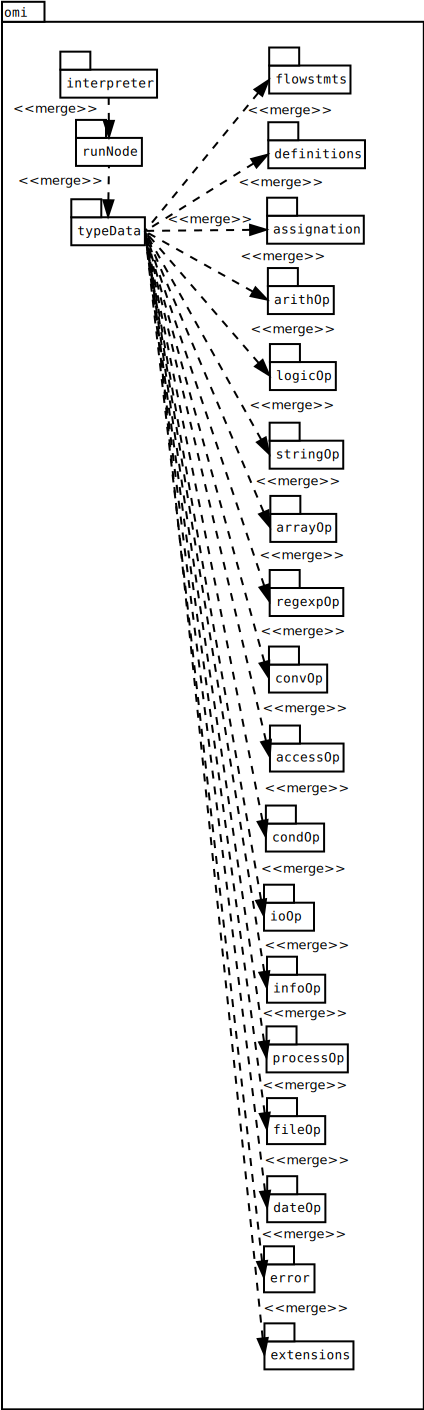
\includegraphics[scale=0.3]{analysis/package-omi.png}
\captionof{figure}{Paquetes OMI}
\end{center}
\end{multicols}
\pagebreak
Este árbol está formado 
por nodos denominados ejecutables, dado que al ser procesados en profundidad se llevará 
a cabo la ejecución del programa. Los nodos ejecutables dan significado semántico a 
cada una de las sentencias que componen el contenido fuente.

El interprete se compone además de un contexto denominado principal, que será sobre el que 
opere de forma predeterminada. Un contexto está formado por una serie de tablas de símbolos 
que serán manipuladas por ciertos nodos ejecutables cuando sean procesados. Estas tablas guardan 
referencias a nodos ejecutables correspondientes a símbolos variables, funciones y clases de objetos 
que son definidos en el código fuente. Existen determinados nodos que al ser ejecutados pueden 
cambiar el contexto en uso.

El interprete es ejecutado con una serie de argumentos que alteran su funcionamiento.

\begin{center}
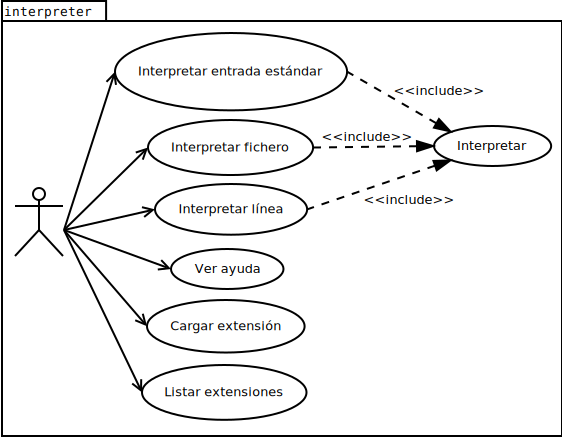
\includegraphics[scale=0.3]{analysis/interpreter.png}
\captionof{figure}{Clases intérprete}
\end{center}
% ----------------------------------------------------------------------
\subsection{Nodos ejecutables}
Se definen un nodo ejecutable para cada aspecto o funcionalidad que contemple el lenguaje.
Cada sentencia se corresponde con un nodo ejecutable, que a su vez puede estar compuestos de otros
nodos. Cada nodo ejecutable guarda el número de nodos que lo referencian para que se pueda hacer un uso 
óptimo del mismo.

Las expresiones son nodos ejecutables que tomarán un valor tras ser procesados. Generalmente forman parte de otros 
nodos correspondientes a sentencias u otras expresiones. El valor que toman pueden ser de un tipo determinado y conocido (numérico, lógico, etc), 
o de tipo indeterminado o no conocido hasta que el nodo es procesado. 

Las expresiones de tipo determinado son extendidas por cada tipo de dato soportado por el lenguaje. Además 
pueden ser consideradas tipos de objetos y estar así asociadas a una clase. De esta forma toda expresión puede disponer
de métodos y atributos según el tipo de dato que guarde.

Las expresiones de tipo indeterminado se componen de una referencia al nodo que guarda el valor tras la ejecución, este podrá ser una 
expresión de tipo determinado.

Las expresiones son nodos imprimibles lo que significa que tienen una representación gráfica asociada que puede ser volcada en la
salida estándar.

\begin{center}
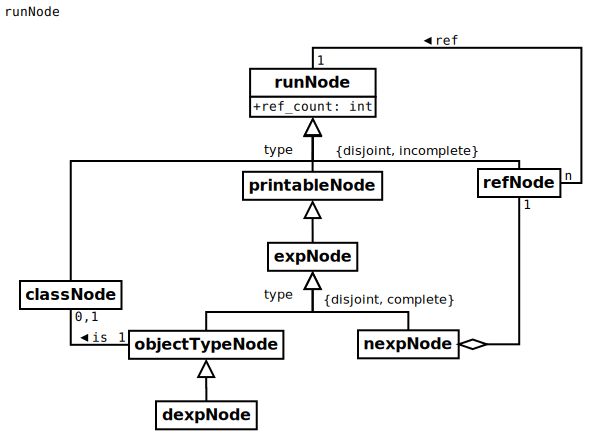
\includegraphics[scale=0.35]{analysis/runNode.png}
\captionof{figure}{Clases nodos ejecutables}
\end{center}
% ----------------------------------------------------------------------
\begin{multicols}{2}
\subsection{Tipos de datos}
Este paquete contiene los nodos que representan expresiones con tipos de datos definidos.
Se describe cada tipo de dato como un nodo con un valor asociado (en algunos casos el tipo puede comprender un único valor).

Muchos nodos son especializaciones de tipos de datos, correspondiéndose con expresiones que 
guardan un valor del tipo de dato al que extienden. Así por ejemplo los nodos de operaciones aritméticas
generalmente extenderán al nodo del mismo tipo de dato. 

Algunos nodos de tipos datos son concretados por nodos que representan un valor constante de dicho tipo de dato.
\columnbreak
\begin{center}
\hfill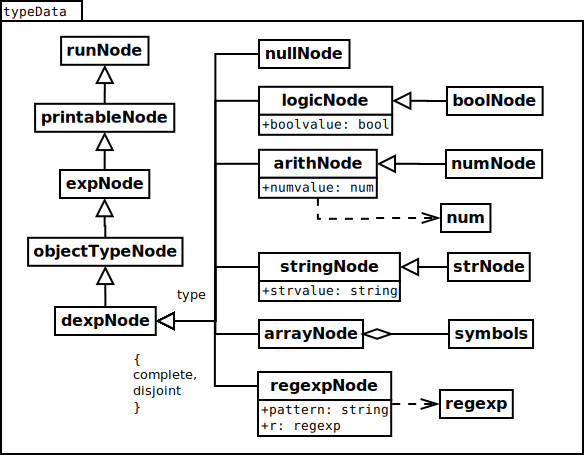
\includegraphics[scale=0.25]{analysis/typeData.png}
\captionof{figure}{Clases tipos de datos}
\end{center}
\end{multicols}
% ----------------------------------------------------------------------

\subsection{Sentencias de control de flujo}
\begin{center}
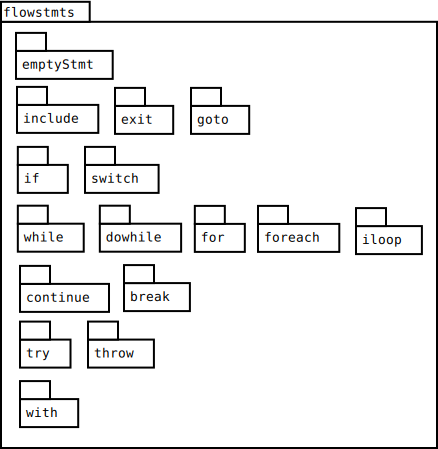
\includegraphics[scale=0.3]{analysis/flowstmts.png}
\captionof{figure}{Paquetes sentencias de control de flujo}
\end{center}

%~ \subsubsection{Sentencia}
\begin{multicols}{2}
\begin{center}
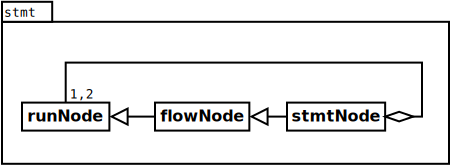
\includegraphics[scale=0.4]{analysis/stmt.png} 
\captionof{figure}{Clases sentencia}
\end{center}
\columnbreak
\begin{center}
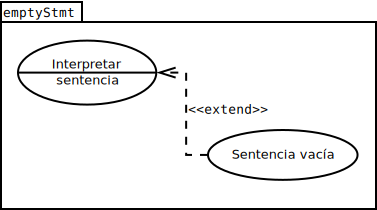
\includegraphics[scale=0.4]{analysis/emptyStmt.png} 
\captionof{figure}{Clases sentencia vacía}
\end{center}
\end{multicols}

\begin{multicols}{2}
%~ \subsubsection{include}
\begin{center}
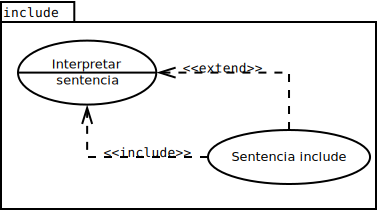
\includegraphics[scale=0.4]{analysis/include.png} 
\captionof{figure}{Clases include}
\end{center}
\columnbreak
%~ \subsubsection{exit}
\begin{center}
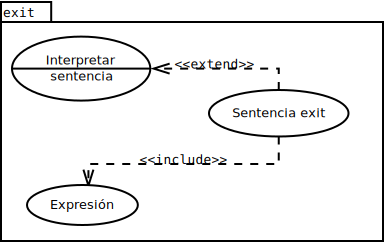
\includegraphics[scale=0.4]{analysis/exit.png} 
\captionof{figure}{Clases exit}
\end{center}
\end{multicols}

\begin{multicols}{2}
%~ \subsubsection{goto}
\begin{center}
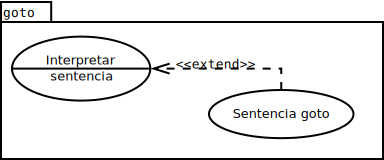
\includegraphics[scale=0.4]{analysis/goto.png} 
\captionof{figure}{Clases goto}
\end{center}
\columnbreak
%~ \subsubsection{if}
\begin{center}
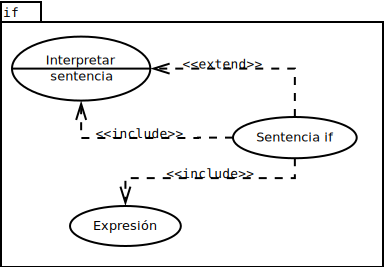
\includegraphics[scale=0.4]{analysis/if.png} 
\captionof{figure}{Clases if}
\end{center}
\end{multicols}

\pagebreak
\begin{multicols}{2}
%~ \subsubsection{switch}
\begin{center}
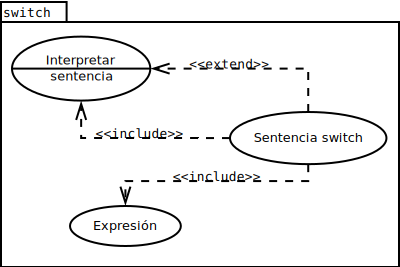
\includegraphics[scale=0.4]{analysis/switch.png} 
\captionof{figure}{Clases switch}
\end{center}
\columnbreak
%~ \subsubsection{while}
\begin{center}
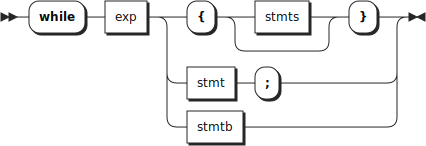
\includegraphics[scale=0.4]{analysis/while.png} 
\captionof{figure}{Clases while}
\end{center}
\end{multicols}

\begin{multicols}{2}
%~ \subsubsection{do...while}
\begin{center}
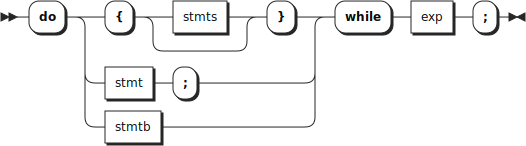
\includegraphics[scale=0.4]{analysis/dowhile.png} 
\captionof{figure}{Clases do...while}
\end{center}
\columnbreak
%~ \subsubsection{for}
\begin{center}
\includegraphics[scale=0.4]{analysis/for.png} 
\captionof{figure}{Clases for}
\end{center}
\end{multicols}

\begin{multicols}{2}
%~ \subsubsection{foreach}
\begin{center}
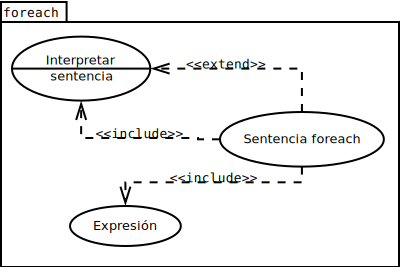
\includegraphics[scale=0.4]{analysis/foreach.png} 
\captionof{figure}{Clases foreach}
\end{center}
\columnbreak
%~ \subsubsection{iloop}
\begin{center}
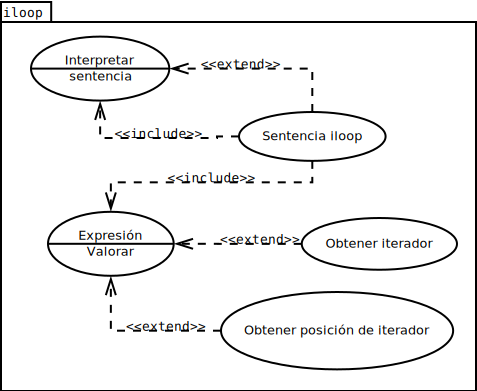
\includegraphics[scale=0.4]{analysis/iloop.png} 
\captionof{figure}{Clases iloop}
\end{center}
\end{multicols}

\begin{multicols}{2}
%~ \subsubsection{continue}
\begin{center}
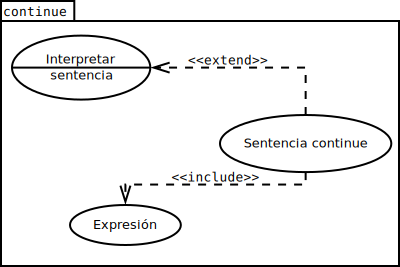
\includegraphics[scale=0.4]{analysis/continue.png} 
\captionof{figure}{Clases continue}
\end{center}
\columnbreak
%~ \subsubsection{break}
\begin{center}
\includegraphics[scale=0.4]{analysis/break.png} 
\captionof{figure}{Clases break}
\end{center}
\end{multicols}

\begin{multicols}{2}
%~ \subsubsection{try}
\begin{center}
\includegraphics[scale=0.4]{analysis/try.png} 
\captionof{figure}{Clases try}
\end{center}
\columnbreak
%~ \subsubsection{throw}
\begin{center}
\includegraphics[scale=0.4]{analysis/throw.png} 
\captionof{figure}{Clases throw}
\end{center}
\end{multicols}

%~ \subsubsection{with}
\begin{center}
\includegraphics[scale=0.4]{analysis/with.png} 
\captionof{figure}{Clases witch}
\end{center}
% ----------------------------------------------------------------------
\subsection {Definiciones}
\begin{center}
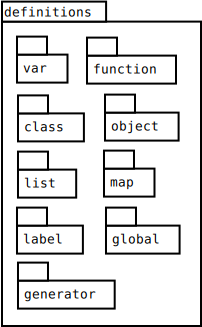
\includegraphics[scale=0.35]{analysis/definitions.png} 
\captionof{figure}{Paquetes definiciones}
\end{center}

%~ \subsubsection {Variables}
\begin{center}
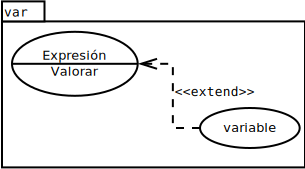
\includegraphics[scale=0.35]{analysis/id.png} 
\captionof{figure}{Clases sobre variables}
\end{center}

%~ \subsubsection {Funciones}
\begin{center}
\includegraphics[scale=0.35]{analysis/functions.png} 
\captionof{figure}{Clases sobre funciones}
\end{center}

%~ \subsubsection {Clases}
\begin{center}
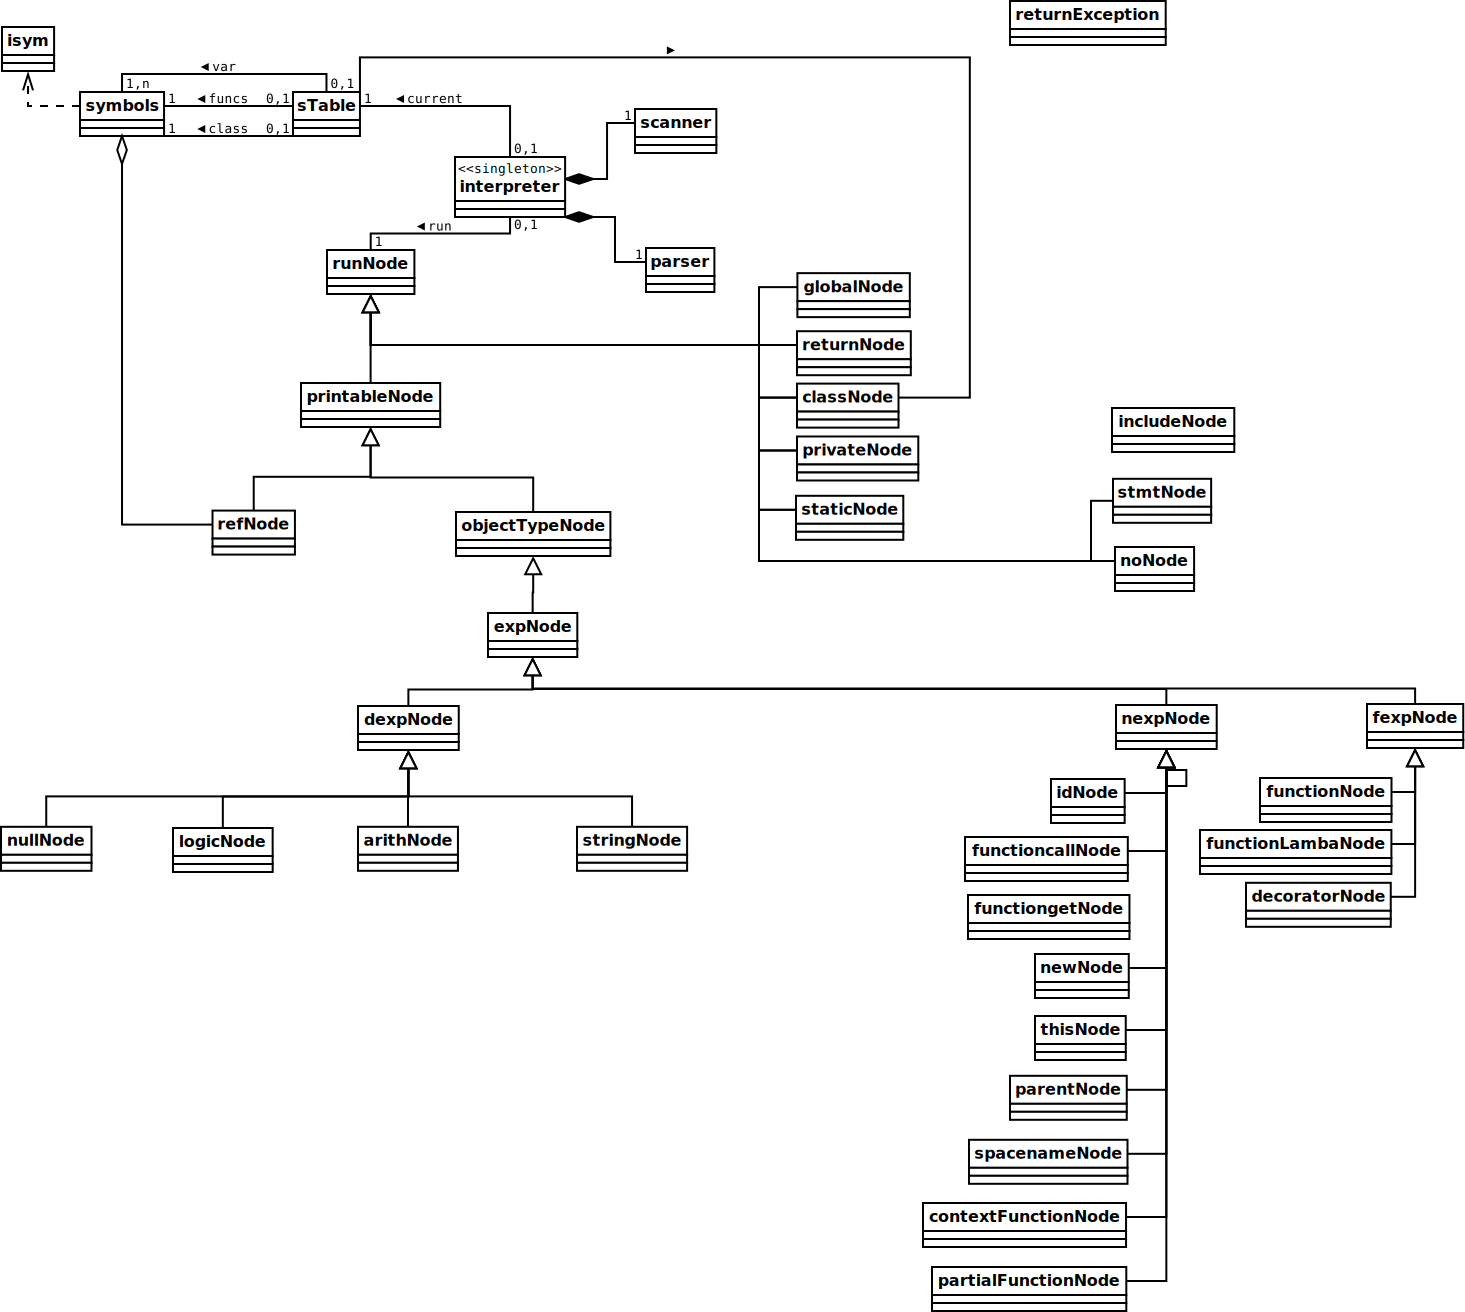
\includegraphics[scale=0.35]{analysis/class.png} 
\captionof{figure}{Clases sobre clases}
\end{center}
\pagebreak

\begin{multicols}{2}
%~ \subsubsection {Objetos}
\begin{center}
\includegraphics[scale=0.3]{analysis/object.png} 
\captionof{figure}{Clases sobre objetos}
\end{center}
\columnbreak
%~ \subsubsection {Listas}
\begin{center}
\includegraphics[scale=0.3]{analysis/list.png} 
\captionof{figure}{Clases sobre listas}
\end{center}
\end{multicols}

\begin{multicols}{2}
%~ \subsubsection {Pares clave/valor}
\begin{center}
\includegraphics[scale=0.3]{analysis/map.png} 
\captionof{figure}{Clases sobre pares clave/valor}
\end{center}
\columnbreak
%~ \subsubsection {Etiquetas}
\begin{center}

\includegraphics[scale=0.3]{analysis/label.png} 
\captionof{figure}{Etiquetas}
\end{center}
\end{multicols}

\begin{multicols}{2}
%~ \subsubsection {Definiciones globales}
\begin{center}
\includegraphics[scale=0.3]{analysis/global.png} 
\captionof{figure}{Definiciones globales}
\end{center}
\columnbreak
%~ \subsubsection {Generadores}
\begin{center}
\includegraphics[scale=0.3]{analysis/generator.png} 
\captionof{figure}{Clases sobre generadores}
\end{center}
\end{multicols}
% ----------------------------------------------------------------------

\subsection {Asignaciones}
\begin{center}
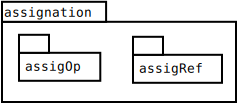
\includegraphics[scale=0.4]{analysis/assig-package.png} 
\captionof{figure}{Paquetes asignaciones}
\end{center}

\begin{multicols}{2}
%~ \subsubsection {Asignación}
\begin{center}
\includegraphics[scale=0.3]{analysis/assigNode.png} 
\captionof{figure}{Clases asignación}
\end{center}
\columnbreak
%~ \subsubsection {Asignación de referencia}
\begin{center}
\includegraphics[scale=0.3]{analysis/assigRef.png} 
\captionof{figure}{Clases asignación de referencia}
\end{center}
\end{multicols}

% ----------------------------------------------------------------------
\subsection {Operadores aritméticos}
\begin{center}
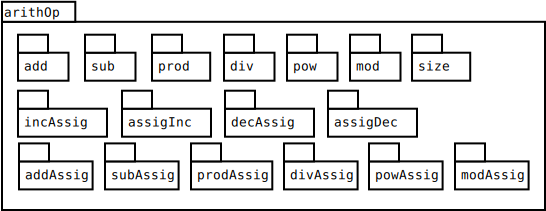
\includegraphics[scale=0.4]{analysis/arithOp-package.png} 
\captionof{figure}{Paquetes operadores aritméticos}
\end{center}

\begin{multicols}{2}
%~ \subsubsection {Suma}
\begin{center}
\includegraphics[scale=0.3]{analysis/add.png} 
\captionof{figure}{Clases suma}
\end{center}
\columnbreak
%~ \subsubsection {Diferencia}
\begin{center}
\includegraphics[scale=0.3]{analysis/sub.png} 
\captionof{figure}{Clases diferencia}
\end{center}
\end{multicols}

\begin{multicols}{2}
%~ \subsubsection {Producto}
\begin{center}
\includegraphics[scale=0.3]{analysis/prod.png} 
\captionof{figure}{Clases producto}
\end{center}
\columnbreak
%~ \subsubsection {División}
\begin{center}
\includegraphics[scale=0.3]{analysis/div.png} 
\captionof{figure}{Clases división}
\end{center}
\end{multicols}
\pagebreak

\begin{multicols}{2}
%~ \subsubsection {Potencia}
\begin{center}
\includegraphics[scale=0.3]{analysis/pow.png} 
\captionof{figure}{Clases potencia}
\end{center}
\columnbreak
%~ \subsubsection {Módulo}
\begin{center}
\includegraphics[scale=0.3]{analysis/mod.png} 
\captionof{figure}{Clases módulo}
\end{center}
\end{multicols}

\begin{multicols}{2}
%~ \subsubsection {Tamaño}
\begin{center}
\includegraphics[scale=0.3]{analysis/size.png} 
\captionof{figure}{Clases tamaño}
\end{center}
\columnbreak
%~ \subsubsection {Incremento y asignación}
\begin{center}
\includegraphics[scale=0.3]{analysis/incAssig.png} 
\captionof{figure}{Clases incremento y asignación}
\end{center}
\end{multicols}

\begin{multicols}{2}
%~ \subsubsection {Asignación e incremento}
\begin{center}
\includegraphics[scale=0.3]{analysis/assigInc.png} 
\captionof{figure}{Clases asignación e incremento}
\end{center}
\columnbreak
%~ \subsubsection {Decremento y asignación}
\begin{center}
\includegraphics[scale=0.3]{analysis/decAssig.png} 
\captionof{figure}{Clases decremento y asignación}
\end{center}
\end{multicols}

%~ \subsubsection {Asignación y decremento}
\begin{center}
\includegraphics[scale=0.3]{analysis/assigDec.png} 
\captionof{figure}{Clases asignación y decremento}
\end{center}
% ----------------------------------------------------------------------

 \subsection {Operadores lógicos}
 \begin{center}
\includegraphics[scale=0.4]{analysis/logicOp-package.png} 
\captionof{figure}{Paquetes operadores lógicos}
\end{center}

\begin{multicols}{2}
%~ \subsubsection {Or}
\begin{center}
\includegraphics[scale=0.3]{analysis/or.png} 
\captionof{figure}{Clases or}
\end{center}
\columnbreak
%~ \subsubsection {And}
\begin{center}
\includegraphics[scale=0.3]{analysis/and.png} 
\captionof{figure}{Clases and}
\end{center}
\end{multicols}

\begin{multicols}{2}
%~ \subsubsection {Negación}
\begin{center}
\includegraphics[scale=0.3]{analysis/not.png} 
\captionof{figure}{Clases negación}
\end{center}
\columnbreak
%~ \subsubsection {Igual que}
\begin{center}
\includegraphics[scale=0.3]{analysis/eq.png} 
\captionof{figure}{Clases igual que}
\end{center}
\end{multicols}
\pagebreak

\begin{multicols}{2}
%~ \subsubsection {Distinto que}
\begin{center}
\includegraphics[scale=0.3]{analysis/neq.png} 
\captionof{figure}{Clases distinto que}
\end{center}
\columnbreak
%~ \subsubsection {Menor que}
\begin{center}
\includegraphics[scale=0.3]{analysis/lth.png} 
\captionof{figure}{Clases menor que}
\end{center}
\end{multicols}

\begin{multicols}{2}
%~ \subsubsection {Menor o igual que}
\begin{center}
\includegraphics[scale=0.3]{analysis/leq.png} 
\captionof{figure}{Clases menor o igual que}
\end{center}
\columnbreak
%~ \subsubsection {Mayor que}
\begin{center}
\includegraphics[scale=0.3]{analysis/gth.png} 
\captionof{figure}{Clases mayor que}
\end{center}
\end{multicols}

\begin{multicols}{2}
%~ \subsubsection {Mayor o igual que}
\begin{center}
\includegraphics[scale=0.3]{analysis/geq.png} 
\captionof{figure}{Clases mayor o igual que}
\end{center}
\columnbreak
%~ \subsubsection {Idéntico a}
\begin{center}
\includegraphics[scale=0.3]{analysis/iden.png} 
\captionof{figure}{Clases idéntico a}
\end{center}
\end{multicols}

\begin{multicols}{2}
%~ \subsubsection {No idéntico a}
\begin{center}
\includegraphics[scale=0.3]{analysis/niden.png} 
\captionof{figure}{Clases no idéntico a}
\end{center}
\columnbreak
%~ \subsubsection {Es nulo}
\begin{center}
\includegraphics[scale=0.3]{analysis/isNull.png} 
\captionof{figure}{Clases es nulo}
\end{center}
\end{multicols}

%~ \subsubsection {Vacío}
\begin{center}
\includegraphics[scale=0.3]{analysis/empty.png} 
\captionof{figure}{Clases vacío}
\end{center}

% ----------------------------------------------------------------------

\subsection {Operadores sobre cadenas}
\begin{center}
\includegraphics[scale=0.3]{analysis/stringOp-package.png} 
\captionof{figure}{Paquetes operadores de cadenas}
\end{center}

\begin{multicols}{2}
%~ \subsubsection {Concatenación}
\begin{center}
\includegraphics[scale=0.3]{analysis/cat.png} 
\captionof{figure}{Clases concatenación}
\end{center}
\columnbreak
%~ \subsubsection {explode}
\begin{center}
\includegraphics[scale=0.3]{analysis/explode.png} 
\captionof{figure}{Clases explode}
\end{center}
\end{multicols}

\begin{multicols}{2}
%~ \subsubsection {implode}
\begin{center}
\includegraphics[scale=0.3]{analysis/implode.png} 
\captionof{figure}{Clases implode}
\end{center}
\columnbreak
%~ \subsubsection {sprintf}
\begin{center}
\includegraphics[scale=0.3]{analysis/sprintf.png} 
\captionof{figure}{Clases sprintf}
\end{center}
\end{multicols}

\begin{multicols}{2}
%~ \subsubsection {Buscar subcadena}
\begin{center}
\includegraphics[scale=0.3]{analysis/find.png} 
\captionof{figure}{Clases buscar subcadena}
\end{center}
\columnbreak
%~ \subsubsection {Buscar y remplazar}
\begin{center}
\includegraphics[scale=0.3]{analysis/replace.png} 
\captionof{figure}{Clases buscar y remplazar}
\end{center}
\end{multicols}

\begin{multicols}{2}
%~ \subsubsection {Remplazar subcadena}
\begin{center}
\includegraphics[scale=0.3]{analysis/subreplace.png} 
\captionof{figure}{Clases remplazar subcadena}
\end{center}
\columnbreak
%~ \subsubsection {Convertir a mayúsculas}
\begin{center}
\includegraphics[scale=0.3]{analysis/upper.png}
\captionof{figure}{Clases convertir a mayúsculas} 
\end{center}
\end{multicols}

%~ \subsubsection {Convertir a minúsculas}
\begin{center}
\includegraphics[scale=0.3]{analysis/lower.png} 
\captionof{figure}{Clases convertir a minúsculas} 
\end{center}

%~ \subsubsection {Concatenación y asignación}
%~ Diagrama aún por realizar.
%~ \begin{center}
%~ \includegraphics[scale=0.4]{analysis/lower.png} \\
%~ \end{center}
% ----------------------------------------------------------------------

\subsection {Operadores sobre array}
\begin{center}
\includegraphics[scale=0.4]{analysis/arrayOp-package.png} 
\captionof{figure}{Paquetes operadores sobre array} 
\end{center}

\begin{multicols}{2}
%~ \subsubsection {Dividir en fragmentos}
\begin{center}
\includegraphics[scale=0.25]{analysis/chunk.png} 
\captionof{figure}{Clases dividir en fragmentos} 
\end{center}
\columnbreak
%~ \subsubsection {Reducir mediante función}
\begin{center}
\includegraphics[scale=0.25]{analysis/reduce.png} 
\captionof{figure}{Clases reducir mediante función} 
\end{center}
\end{multicols}

\begin{multicols}{2}
%~ \subsubsection {Obtener último}
\begin{center}
\includegraphics[scale=0.35]{analysis/last.png} 
\captionof{figure}{Clases obtener último} 
\end{center}
\columnbreak
%~ \subsubsection {Obtener primero}
\begin{center}
\includegraphics[scale=0.35]{analysis/first.png} 
\captionof{figure}{Clases obtener primero} 
\end{center}
\end{multicols}

\begin{multicols}{2}
%~ \subsubsection {Insertar en posición}
\begin{center}
\includegraphics[scale=0.35]{analysis/insert.png} 
\captionof{figure}{Clases insertar en posición} 
\end{center}
\columnbreak
%~ \subsubsection {Eliminar posición}
\begin{center}
\includegraphics[scale=0.35]{analysis/delete.png} 
\captionof{figure}{Clases eliminar posición} 
\end{center}
\end{multicols}

\begin{multicols}{2}
%~ \subsubsection {Insertar al inicio}
\begin{center}
\includegraphics[scale=0.35]{analysis/unshift.png} 
\captionof{figure}{Clases insertar al inicio}
\end{center}
\columnbreak
%~ \subsubsection {Insertar al final}
\begin{center}
\includegraphics[scale=0.35]{analysis/push.png} 
\captionof{figure}{Clases insertar al final}
\end{center}
\end{multicols}

\begin{multicols}{2}
%~ \subsubsection {Eliminar del inicio}
\begin{center}
\includegraphics[scale=0.35]{analysis/shift.png} 
\captionof{figure}{Clases eliminar del inicio}
\end{center}
\columnbreak
%~ \subsubsection {Eliminar del final}
\begin{center}
\includegraphics[scale=0.35]{analysis/pop.png} 
\captionof{figure}{Clases eliminar del final}
\end{center}
\end{multicols}

% ----------------------------------------------------------------------

\subsection {Operadores sobre expresiones regulares}
\begin{center}
\includegraphics[scale=0.4]{analysis/regexpOp-package.png} 
\captionof{figure}{Paquetes operadores sobre expresiones regulares}
\end{center}

\begin{multicols}{2}
%~ \subsubsection {Crear expresión regular}
\begin{center}
\includegraphics[scale=0.25]{analysis/newRegExp.png}
\captionof{figure}{Clases crear expresión regular} 
\end{center}
\columnbreak
%~ \subsubsection {match}
\begin{center}
\includegraphics[scale=0.3]{analysis/match.png} 
\captionof{figure}{Clases match}
\end{center}
\end{multicols}

%~ \subsubsection {search}
\begin{center}
\includegraphics[scale=0.3]{analysis/search.png} 
\captionof{figure}{Clases search}
\end{center}

% ----------------------------------------------------------------------

\subsection {Conversión de tipos}
\begin{center}
\includegraphics[scale=0.3]{analysis/convOp-package.png} 
\captionof{figure}{Paquetes conversión de tipos}
\end{center}

\begin{multicols}{2}
%~ \subsubsection {Conversión a lógico}
\begin{center}
\includegraphics[scale=0.35]{analysis/boolconv.png} 
\captionof{figure}{Clases conversión a lógico}
\end{center}
\columnbreak
%~ \subsubsection {Conversión a entero}
\begin{center}
\includegraphics[scale=0.35]{analysis/intconv.png} 
\captionof{figure}{Clases conversión a entero}
\end{center}
\end{multicols}

\begin{multicols}{2}
%~ \subsubsection {Conversión a flotante}
\begin{center}
\includegraphics[scale=0.35]{analysis/floatconv.png} 
\captionof{figure}{Clases conversión a flotante}
\end{center}
\columnbreak
%~ \subsubsection {Conversión a cadena}
\begin{center}
\includegraphics[scale=0.35]{analysis/strconv.png} 
\captionof{figure}{Clases conversión a cadena}
\end{center}
\end{multicols}
% ----------------------------------------------------------------------

\subsection {Operadores de acceso}
\begin{center}
\includegraphics[scale=0.4]{analysis/accessOp-package.png} 
\captionof{figure}{Paquetes operadores de acceso}
\end{center}

\begin{multicols}{2}
%~ \subsubsection {Acceso a clave} 
\begin{center}
\includegraphics[scale=0.3]{analysis/get.png} 
\captionof{figure}{Clases acceso a clave}
\end{center}
\columnbreak
%~ \subsubsection {Acceso a función} 
\begin{center}
\includegraphics[scale=0.3]{analysis/getFunc.png} 
\captionof{figure}{Clases acceso a función}
\end{center}
\end{multicols}

%~ \subsubsection {Acceso a variable de entorno} 
\begin{center}
\includegraphics[scale=0.3]{analysis/getEnvSys.png} 
\captionof{figure}{Clases acceso a variable de entorno}
\end{center}
% ----------------------------------------------------------------------

\subsection {Operadores condicionales} 
\begin{center}
\includegraphics[scale=0.4]{analysis/condOp-package.png} 
\captionof{figure}{Paquetes Operadores condicionales}
\end{center}

\begin{multicols}{2}
%~ \subsubsection {Ternario} 
\begin{center}
\includegraphics[scale=0.3]{analysis/tern.png} 
\captionof{figure}{Clases ternario}
\end{center}
\columnbreak
%~ \subsubsection {Fusión de nulos} 
\begin{center}
\includegraphics[scale=0.3]{analysis/nullCoalescing.png} 
\captionof{figure}{Clases fusión de nulos}
\end{center}
\end{multicols}

% ----------------------------------------------------------------------

\subsection {Operadores de entrada/salida} 
\begin{center}
\includegraphics[scale=0.4]{analysis/ioOp-package.png} 
\captionof{figure}{Paquetes operadores de entrada/salida}
\end{center}

\pagebreak
\begin{multicols}{2}
%~ \subsubsection {Salida estándar} 
\begin{center}
\includegraphics[scale=0.3]{analysis/output.png} 
\captionof{figure}{Clases salida estándar}
\end{center}
\columnbreak
%~ \subsubsection {Entrada estándar} 
\begin{center}
\includegraphics[scale=0.3]{analysis/input.png} 
\captionof{figure}{Clases entrada estándar}
\end{center}
\end{multicols}

% ----------------------------------------------------------------------

\subsection {Operadores informativos} 
\begin{center}
\includegraphics[scale=0.4]{analysis/infoOp-package.png} 
\captionof{figure}{Paquetes operadores informativos}
\end{center}

\begin{multicols}{2}
%~ \subsubsection {Tipo de} 
\begin{center}
\includegraphics[scale=0.3]{analysis/typeOf.png} 
\captionof{figure}{Clases tipo de}
\end{center}
\columnbreak
%~ \subsubsection {Tamaño de} 
\begin{center}
\includegraphics[scale=0.3]{analysis/sizeOf.png} 
\captionof{figure}{Clases tamaño de}
\end{center}
\end{multicols}

%~ \subsubsection {Información sobre} 
\begin{center}
\includegraphics[scale=0.3]{analysis/datInfo.png} 
\captionof{figure}{Clases información sobre}
\end{center}
% ----------------------------------------------------------------------

\subsection {Procesos} 
\begin{center}
\includegraphics[scale=0.4]{analysis/processOp-package.png} 
\captionof{figure}{Paquete de procesos}
\end{center}

\begin{multicols}{2}
%~ \subsubsection {Crear proceso} 
\begin{center}
\includegraphics[scale=0.3]{analysis/fork.png} 
\captionof{figure}{Clases crear proceso}
\end{center}
\columnbreak
%~ \subsubsection {Esperar finalización} 
\begin{center}
\includegraphics[scale=0.3]{analysis/wait.png} 
\captionof{figure}{Clases esperar finalización}
\end{center}
\end{multicols}

\begin{multicols}{2}
%~ \subsubsection {Obtener identificador } 
\begin{center}
\includegraphics[scale=0.3]{analysis/getpid.png} 
\captionof{figure}{Clases obtener identificador}
\end{center}
\columnbreak
%~ \subsubsection {Obtener identificador padre} 
\begin{center}
\includegraphics[scale=0.3]{analysis/getppid.png} 
\captionof{figure}{Clases obtener identificador padre}
\end{center}
\end{multicols}

\begin{multicols}{2}
%~ \subsubsection {Ejecutar como proceso} 
\begin{center}
\includegraphics[scale=0.3]{analysis/process.png} 
\captionof{figure}{Clases ejecutar como proceso}
\end{center}
\columnbreak
%~ \subsubsection {Salir de proceso} 
\begin{center}
\includegraphics[scale=0.3]{analysis/exitProcess.png} 
\captionof{figure}{Clases salir de proceso}
\end{center}
\end{multicols}

\pagebreak

\begin{multicols}{2}
%~ \subsubsection {Señal a proceso} 
\begin{center}
\includegraphics[scale=0.3]{analysis/signal.png} 
\captionof{figure}{Clases señal a proceso}
\end{center}
\columnbreak
%~ \subsubsection {Manejador de señales} 
\begin{center}
\includegraphics[scale=0.3]{analysis/signalhandler.png} 
\captionof{figure}{Clases manejador de señales}
\end{center}
\end{multicols}

\begin{multicols}{2}
%~ \subsubsection {Evaluar cadena} 
\begin{center}
\includegraphics[scale=0.3]{analysis/eval.png} 
\captionof{figure}{Clases evaluar cadena}
\end{center}
\columnbreak
%~ \subsubsection {Ejecutar comando del sistema} 
\begin{center}
\includegraphics[scale=0.3]{analysis/exec.png} 
\captionof{figure}{Clases ejecutar comando del sistema}
\end{center}
\end{multicols}
% ----------------------------------------------------------------------

\subsection {Ficheros} 
\begin{center}
\includegraphics[scale=0.4]{analysis/fileOp-package.png} 
\captionof{figure}{Paquetes de ficheros}
\end{center}

\begin{multicols}{2}
%~ \subsubsection {Obtener un flujo a fichero} 
\begin{center}
\includegraphics[scale=0.3]{analysis/file.png} 
\captionof{figure}{Clases obtener un flujo a fichero}
\end{center}
\columnbreak
%~ \subsubsection {Escribir en flujo a fichero} 
\begin{center}
\includegraphics[scale=0.3]{analysis/fput.png} 
\captionof{figure}{escribir en flujo a fichero}
\end{center}
\end{multicols}

\begin{multicols}{2}
%~ \subsubsection {Leer de flujo a fichero} 
\begin{center}
\includegraphics[scale=0.3]{analysis/fget.png} 
\captionof{figure}{Clases leer de flujo a fichero}
\end{center}
\columnbreak
%~ \subsubsection {Cambiar posición en fichero} 
\begin{center}
\includegraphics[scale=0.3]{analysis/fseek.png} 
\captionof{figure}{Clases cambiar posición en fichero}
\end{center}
\end{multicols}

\begin{multicols}{2}
%~ \subsubsection {Obtener posición en flujo a fichero} 
\begin{center}
\includegraphics[scale=0.3]{analysis/ftell.png} 
\captionof{figure}{Clases obtener posición en flujo a fichero}
\end{center}
\columnbreak
%~ \subsubsection {Cerrar flujo a fichero} 
\begin{center}
\includegraphics[scale=0.3]{analysis/fclose.png} 
\captionof{figure}{Clases cerrar flujo a fichero}
\end{center}
\end{multicols}

\begin{multicols}{2}
%~ \subsubsection {Leer fichero} 
\begin{center}
\includegraphics[scale=0.3]{analysis/fread.png} 
\captionof{figure}{Clases leer fichero}
\end{center}
\columnbreak
%~ \subsubsection {Escribir en fichero} 
\begin{center}
\includegraphics[scale=0.3]{analysis/fwrite.png} 
\captionof{figure}{Clases escribir en fichero}
\end{center}
\end{multicols}

%~ \subsubsection {Escribir al final de fichero} 
\begin{center}
\includegraphics[scale=0.3]{analysis/fappend.png} 
\captionof{figure}{Clases escribir al final de fichero}
\end{center}
% ----------------------------------------------------------------------
 \pagebreak

\subsection {Fechas}
\begin{center}
\includegraphics[scale=0.4]{analysis/dateOp-package.png} 
\captionof{figure}{Paquetes de fechas}
\end{center}

\begin{multicols}{2}
%~ \subsubsection {Tiempo Unix} 
\begin{center}
\includegraphics[scale=0.35]{analysis/time.png} 
\captionof{figure}{Clases tiempo Unix}
\end{center}
\columnbreak
%~ \subsubsection {Fecha y hora con formato} 
\begin{center}
\includegraphics[scale=0.35]{analysis/date.png} 
\captionof{figure}{Clases fecha y hora con formato}
\end{center}
\end{multicols}

%~ \subsubsection {sleep} 
\begin{center}
\includegraphics[scale=0.35]{analysis/sleep.png} 
\captionof{figure}{Clases sleep}
\end{center}

% ----------------------------------------------------------------------

\subsection {Errores} 
%~ \begin{center}
%~ \includegraphics[scale=0.4]{analysis/error-package.png} \\
%~ \end{center}
%~ 
%~ \subsubsection {Error} 
\begin{center}
\includegraphics[scale=0.35]{analysis/errorException.png} 
\captionof{figure}{Clases Errores}
\end{center}

%~ \subsubsection {Manejador de errores } 
%~ Diagrama aún por realizar
%~ \begin{center}
%~ \includegraphics[scale=0.4]{analysis/errorhandler.png} \\
%~ \end{center}

%~ \subsubsection {Manejador de excepciones no capturadas} 
%~ Diagrama aún por realizar
%~ \begin{center}
%~ \includegraphics[scale=0.4]{analysis/errorhandler.png} \\
%~ \end{center}
% ----------------------------------------------------------------------


\subsection {Extensiones} 
\begin{center}
\includegraphics[scale=0.35]{analysis/extensions-package.png} 
\captionof{figure}{Paquete de extensiones}
\end{center}

%~ \subsection {plugins}
\begin{center}
\includegraphics[scale=0.35]{analysis/plugins.png} 
\captionof{figure}{Clases plugins}
\end{center}

\subsubsection{Biblioteca GNU de internacionalización (gettext)}
\begin{center}
\includegraphics[scale=0.4]{analysis/gettext-ext-package.png} 
\captionof{figure}{Paquetes de Biblioteca GNU de internacionalización (gettext)}
\end{center}

%~ \paragraph {gettext}
\begin{center}
\includegraphics[scale=0.35]{analysis/gettext.png} 
\captionof{figure}{Clases gettext}
\end{center}

\begin{multicols}{2}
%~ \paragraph {setlocale}
\begin{center}
\includegraphics[scale=0.35]{analysis/setlocale.png} 
\captionof{figure}{Clases setlocale}
\end{center}
%~ \paragraph {dgettext}
\begin{center}
\includegraphics[scale=0.35]{analysis/dgettext.png} 
\captionof{figure}{Clases dgettext}
\end{center}
\columnbreak
%~ \paragraph {bindtextdomain}
\begin{center}
\includegraphics[scale=0.35]{analysis/bindtextdomain.png} 
\captionof{figure}{Clases bindtextdomain}
\end{center}
%~ \paragraph {textdomain}
\begin{center}
\includegraphics[scale=0.35]{analysis/textdomain.png} 
\captionof{figure}{Clases textdomain}
\end{center}
\end{multicols}

\subsection {rTree} 
El intérprete OMI tiene la capacidad de generar una salida relativa
a su estado y funcionamiento. Para completar el proyecto se precisa 
de una herramienta capaz de interpretar y representar este estado 
interno de forma gráfica y textual. 

El modelo de datos del cliente OMI se define de forma similar al intérprete.
La principal diferencia es que en el intérprete este modelo de datos se usa para procesar y 
ejecutar el código fuente, mientras que en el cliente se usa para representar gráficamente 
el proceso llevado a cabo. Es por ello que el modelo de datos del cliente es más abstracto. 

\begin{center}
\includegraphics[scale=0.6]{analysis/rtree.png} 
\captionof{figure}{Clases rTree}
\end{center}

%~ \subsubsection {Operaciones sobre un SGBD Mysql}
%~ \begin{center}
%~ \includegraphics[scale=0.4]{analysis/mysql-ext-package.png} \\
%~ \end{center}
%~ \paragraph {Abrir conexión}
%~ \begin{center}
%~ \includegraphics[scale=0.4]{analysis/db.png} \\
%~ \end{center}
%~ 
%~ \paragraph {Consulta}
%~ \begin{center}
%~ \includegraphics[scale=0.4]{analysis/dbQuery.png} \\
%~ \end{center}
%~ 
%~ \paragraph {Cerrar conexión}
%~ Diagrama aún por realizar.
%~ \begin{center}
%~ \includegraphics[scale=0.4]{analysis/dbClose.png} \\
%~ \end{center}
%~ 
%~ \paragraph {Insertar datos}
%~ \begin{center}
%~ \includegraphics[scale=0.4]{analysis/dbInsert.png} \\
%~ \end{center}
%~ 
%~ \paragraph {Seleccionar datos}
%~ \begin{center}
%~ \includegraphics[scale=0.4]{analysis/dbSelect.png} \\
%~ \end{center}
%~ 
%~ \paragraph {Actualizar datos}
%~ \begin{center}
%~ \includegraphics[scale=0.4]{analysis/dbUpdate.png} \\
%~ \end{center}
%~ 
%~ \paragraph {Eliminar datos}
%~ \begin{center}
%~ \includegraphics[scale=0.4]{analysis/dbDelete.png} \\
%~ \end{center}
%~ 
%~ % ----------------------------------------------------------------------


% ======================================================================
\section{Modelo de casos de uso}
%~ En el presente documento se detallan los casos de uso recogidos para el 
%~ interprete OMI. Para ello los casos de uso son distribuidos
%~ en paquetes, y estos modelados mediante un diagrama. 
%~ 
%~ El diagrama de paquetes inicial presenta una organización y distribución 
%~ general de los paquetes en los que se ha dividido el modelo. Estos paquetes
%~ pueden contener diagramas de casos de uso u otros paquetes. Además se establecen
%~ relaciones entre estos.
%~ 
%~ La relación de mezcla (merge) entre dos paquetes significa que el contenido
%~ de ambos paquetes será superpuesto, cumplimentando la información que presenta uno
%~ con la que ofrece el otro. 
%~ 
%~ Inicialmente se presenta el paquete ``interpreter'' que recoge los casos 
%~ de uso que puede llevar a cabo el usuario. Aquí el caso de uso que cabría 
%~ destacar es el de Interpretar. Este consiste en la interpretación sentencia 
%~ a sentencia del código fuente facilitado por el usuario. Este caso de
%~ uso es extendido según el tipo de sentencia interpretada en cada momento.
En esta sección se detallan los casos de usos que recogen los sistemas que conforman el proyecto OMI. 
Un caso de uso describe la secuencia de  interacciones entre el sistema y sus
actores como consecuencia de un evento. 

En primer lugar se describen los actores que hacen uso del sistema, llegándose a distinguir dos que serán nominados 
usuario y sistema externo. Luego se describen los casos de uso del sistema intérprete y del cliente runTree. 

\subsection{Actores}
Los actores humanos que interactúan con los sistemas OMI presentan todos un mismo rol. Así el 
único actor definido será llamado usuario.  Los usuarios que hacen uso del intérprete pueden ser desarrolladores,
estudiantes u otros perfiles técnicos, pero todos usarán el sistema de la misma forma.

Por otro lado el intérprete OMI puede ser usado por otros sistemas, viéndose estos actores de determinados casos
de uso. Algunos sistemas del proyecto OMI hacen uso del intérprete para llevar  a cabo su propósito.

%~ En primer lugar se describen los casos de usos del intérprete OMI. El principal caso de uso es
%~ el de intérpretar, ya que recoge el proceso principal.  

%~ \begin{center}
%~ \includegraphics[scale=0.3]{analysis/package-omi.png} \\
%~ \end{center}
% ======================================================================
\subsection{Intérprete}
\begin{center}
\includegraphics[scale=0.5]{analysis/use_case_interpreter.png} 
\captionof{figure}{Casos de usos intérprete}
\end{center}
% ----------------------------------------------------------------------
\subsubsection{Casos de usos interpretar entrada estándar}

\begin{description}
  \item[Caso de Uso:] 
  Interpretar entrada estándar.
  \item[Tipo:] General.
  \item[Descripción:] 
  El usuario introduce un bloque de código en forma de cadena de 
  caracteres mediante la entrada estándar. El sistema lo interpreta 
  y ejecuta.
  \item[Actores:] 
  Usuario.
  \item[Precondiciones:] 
  El sistema debe estar esperando un bloque de código mediante la entrada estándar.
  \item[Postcondiciones:] 
  El código introducido es interpretado y ejecutado.
  \item[Escenario principal:] \hfill 
  \begin{enumerate}
   \item El usuario inicia el sistema facilitando un listado de argumentos.
   \item El sistema asigna como variables cada argumento y solicita contenido fuente al usuario. 
   \item El usuario introduce un bloque de código en la entrada estándar.
   \item El sistema obtiene el bloque de código a interpretar mediante la entrada estándar.
   \item Incluir (Interpretar). 
  \end{enumerate}
\end{description}
% ----------------------------------------------------------------------
\subsubsection{Interpretar fichero}

\begin{description}
   \item[Caso de Uso:]  Interpretar fichero.
   \item[Tipo:] General.
   \item[Descripción:] 
   El usuario indica un fichero que contiene código y que será 
   interpretado y ejecutado por el sistema.
   \item[Actores:] 
   Usuario.
   \item[Precondiciones:] 
   El sistema espera que se le indique un fichero.
   \item[Postcondiciones:] 
   El fichero es leído y el código en el mismo es interpretado y ejecutado.
   \item[Escenario principal:] \hfill
   \begin{enumerate}
   \item El usuario indica la ruta a un fichero y una serie de argumentos
   \item El sistema lee el fichero y obtiene el código en el mismo, además asigna cada argumento a variables.
   \item Incluir (Interpretar).
   \end{enumerate}
   
   \item[Flujo alternativo:] \hfill 
   \begin{enumerate} \itemsep1pt \parskip0pt \parsep0pt
   \setcounter{enumi}{1}
   \renewcommand{\labelenumi}{}
   \renewcommand{\labelenumiii}{\arabic{enumiii}.}
   \renewcommand{\labelenumii}{\arabic{enumi}\alph{enumii}.}
      \item 
      \begin {enumerate}
         \setcounter{enumii}{0}
         \item El fichero indicado no se encuentra.
         \begin{enumerate}
         \item El sistema informa del error y finaliza.
         \end{enumerate}
      \end{enumerate}
   \end{enumerate}
\end{description}

% ----------------------------------------------------------------------
\subsubsection{Interpretar línea}

\begin{description}
   \item[Caso de Uso:]  Interpretar línea.
   \item[Tipo:] General.
   \item[Descripción:] 
   El usuario introduce bloques de códigos denominados líneas
   de una forma interactiva. El sistema solicita por la entrada 
   estándar las líneas de código, que serán interpretadas y ejecutadas.
   \item[Actores:] 
   Usuario.
   \item[Precondiciones:] 
   El sistema se encuentra en modo interactivo.
   \item[Postcondiciones:] 
   Se interpreta cada línea introducida por el usuario
   \item[Escenario principal:] \hfill
   \begin{enumerate}
   \item El usuario inicia el sistema facilitando un listado de argumentos y la opción de interprete de línea.
   \item El sistema asigna como variables cada argumento y muestra un prompt que indica que espera una línea de código.
   \item El usuario introduce una línea de código.
   \item El sistema lee de la entrada estándar la línea introducida.
   \item Include (Interpretar). \\\\\hfill\hfill
   El sistema repite el caso de uso hasta que se interpreta una sentencia que produzca 
   la salida.
   \end{enumerate}
\end{description}

% ----------------------------------------------------------------------
\subsubsection{Interpretar}

\begin{description}
   \item[Caso de Uso:]  Interpretar.
   \item[Tipo:] General.
   \item[Nivel:]  Subfunción.
   \item[Descripción:] 
   El sistema analiza, interpreta y ejecuta un bloque de código facilitado por el usuario.
   Para ello comprueba que este cumple con el léxico y la gramática del lenguaje 
   que define, dividiéndolo a su vez en sentencias que serán interpretadas. 
   \item[Precondiciones:] 
   Se dispone de un bloque de código.
   \item[Postcondiciones:] 
   El bloque de código es interpretado.
   %~ \item [Puntos de extensión:] \hfill
   %~ \begin{description}
      %~ \item[Sentencia:] Según el tipo de sentencia.
   %~ \end{description}
   \item[Escenario principal:] \hfill
   \begin{enumerate}
   \item El sistema procesa y comprueba el bloque de código, aplicando
   la gramática y léxico que define.
   \item El sistema obtiene e interpreta cada sentencia en el código, produciéndose
   el significado semántico que estas encierran.
   \end{enumerate}
   \item[Flujo alternativo:] \hfill 
   \begin{enumerate} \itemsep1pt \parskip0pt \parsep0pt
   \setcounter{enumi}{0}
   \renewcommand{\labelenumi}{}
   \renewcommand{\labelenumiii}{\arabic{enumiii}.}
   \renewcommand{\labelenumii}{\arabic{enumi}\alph{enumii}.}
      \item 
      \begin {enumerate}
         \setcounter{enumii}{0}
         \item El código no respeta el léxico del lenguaje.
         \begin{enumerate}
         \item El sistema informa del error y finaliza.
         \end{enumerate}
      \end{enumerate}
   \end{enumerate}
   \begin{enumerate} \itemsep1pt \parskip0pt \parsep0pt
   \setcounter{enumi}{0}
   \renewcommand{\labelenumi}{}
   \renewcommand{\labelenumiii}{\arabic{enumiii}.}
   \renewcommand{\labelenumii}{\arabic{enumi}\alph{enumii}.}
      \item 
      \begin {enumerate}
         \setcounter{enumii}{1}
         \item El código no respeta la gramática del lenguaje.
         \begin{enumerate}
         \item El sistema informa del error y finaliza.
         \end{enumerate}
      \end{enumerate}
   \end{enumerate}
   \begin{enumerate} \itemsep1pt \parskip0pt \parsep0pt
   \setcounter{enumi}{1}
   \renewcommand{\labelenumi}{}
   \renewcommand{\labelenumiii}{\arabic{enumiii}.}
   \renewcommand{\labelenumii}{\arabic{enumi}\alph{enumii}.}
      \item 
      \begin {enumerate}
         \setcounter{enumii}{0}
         \item El código no contiene ninguna sentencia.
         \begin{enumerate}
         \item El sistema finaliza.
         \end{enumerate}
      \end{enumerate}
   \end{enumerate}
\end{description}

% ----------------------------------------------------------------------
\subsubsection{Ver ayuda}

\begin{description}
   \item[Caso de Uso:]  Ver ayuda.
   \item[Tipo:] General.
   \item[Descripción:] 
   Se muestra una ayuda que detalla cada opción disponible en el sistema.
   \item[Actores:] 
   Usuario.
   \item[Precondiciones:] 
   Sin precondiciones.
   \item[Postcondiciones:] 
   El sistema muestra un listado que presenta las distintas opciones.
   \item[Escenario principal:] \hfill
   \begin{enumerate}
   \item El usuario indica que quiere visualizar la ayuda.
   \item El sistema muestra un listado completo de las opciones que
   presenta. 
   \end{enumerate}
\end{description}

% ----------------------------------------------------------------------
\subsubsection{Cargar extensión}

\begin{description}
   \item[Caso de Uso:]  Cargar extensión.
   \item[Tipo:] General.
   \item[Descripción:] 
   El usuario indica que una extensión que será cargada por
   el sistema.
   \item[Actores:] 
   Usuario.
   \item[Precondiciones:] 
   Sin precondiciones.
   \item[Postcondiciones:] 
   El sistema cargar la extensión facilitada.
   \item[Escenario principal:] \hfill
   \begin{enumerate}
   \item El usuario indica la ruta a la extensión que desea cargar.
   \item El sistema carga la extensión para disponer de las distintas opciones que 
   ofrece. 
   \end{enumerate}
   \item[Flujo alternativo:] \hfill 
   \begin{enumerate} \itemsep1pt \parskip0pt \parsep0pt
   \setcounter{enumi}{1}
   \renewcommand{\labelenumi}{}
   \renewcommand{\labelenumiii}{\arabic{enumiii}.}
   \renewcommand{\labelenumii}{\arabic{enumi}\alph{enumii}.}
      \item 
      \begin {enumerate}
         \setcounter{enumii}{0}
         \item La extensión indicada no se encuentra.
         \begin{enumerate}
         \item El sistema informa del error.
         \end{enumerate}
      \end{enumerate}
   \end{enumerate}
   \begin{enumerate} \itemsep1pt \parskip0pt \parsep0pt
   \setcounter{enumi}{1}
   \renewcommand{\labelenumi}{}
   \renewcommand{\labelenumiii}{\arabic{enumiii}.}
   \renewcommand{\labelenumii}{\arabic{enumi}\alph{enumii}.}
      \item 
      \begin {enumerate}
         \setcounter{enumii}{1}
         \item La extensión indicada no es una extensión válida.
         \begin{enumerate}
         \item El sistema informa del error.
         \end{enumerate}
      \end{enumerate}
   \end{enumerate}
\end{description}

% ----------------------------------------------------------------------
\subsubsection{Listar extensiones}

\begin{description}
   \item[Caso de Uso:]  Listar extensiones.
   \item[Tipo:] General.
   \item[Descripción:] 
   Lista las extensiones que serán cargadas en cada ejecución del sistema.
   \item[Actores:] 
   Usuario.
   \item[Precondiciones:] 
   Sin precondiciones.
   \item[Postcondiciones:] 
   El sistema lista las extensiones que serán cargadas.
   \item[Escenario principal:] \hfill
   \begin{enumerate}
   \item El usuario indica que desea listar las extensiones cargadas.
   \item El sistema lista las extensiones cargadas por defecto. 
   \end{enumerate}
\end{description}

% ----------------------------------------------------------------------

%~ % ======================================================================
%~ 
%~ \pagebreak
%~ \subsection {Expresiones}
%~ \begin{center}
%~ \includegraphics[scale=0.5]{analysis/exp.png} \\
%~ \end{center}
%~ % ----------------------------------------------------------------------
%~ 
%~ \begin{framed}
%~ \FloatBarrier
%~ \begin{description}
   %~ \item[Caso de Uso:]  Expresión.
   %~ \item[Tipo:] General.
   %~ \item[Nivel:]  Subfunción.
   %~ \item[Descripción:] 
   %~ El sistema valora la expresión según la prioridad de operadores
   %~ que define. 
   %~ \item[Precondiciones:] 
   %~ La expresión cumple con el léxico y gramática del lenguaje.
   %~ \item[Postcondiciones:] 
   %~ El sistema interpreta la expresión obteniendo su valor asociado.
   %~ \item[Puntos de extensión:] \hfill
      %~ \begin{description}
         %~ \item [Valorar:] Según tipo de operador o subexpresión
      %~ \end{description}
   %~ \item[Escenario principal:] \hfill
   %~ \begin{enumerate}
   %~ \item El sistema determina el operador 
   %~ o subexpresión de mayor prioridad.
   %~ \item Valorar: punto de extensión 
   %~ \end{enumerate}
%~ \end{description}
 %~ \FloatBarrier
%~ \end{framed}
%~ % ----------------------------------------------------------------------
%~ % ======================================================================
%~ 
%~ 
%~ \subsection {Tipos de datos}
%~ \begin{center}
%~ \includegraphics[scale=0.4]{analysis/dataType.png} \\
%~ \end{center}
%~ % ----------------------------------------------------------------------
%~ \subsubsection{Valorar constante nula}
%~ \begin{framed}
%~ \FloatBarrier
%~ \begin{description}
   %~ \item[Caso de Uso:] Valorar constante nula.
   %~ \item [Tipo:] Expresión.
   %~ \item[Nivel:]  Subfunción.
   %~ \item[Descripción:] 
   %~ El sistema valora una expresión o subexpresión correspondiente a
   %~ la constante nula codificada de forma explicita.
   %~ \item[Precondiciones:] 
   %~ El sistema se encuentra valorando una expresión y esta es un valor constante nulo.
   %~ \item[Postcondiciones:] 
   %~ El sistema atribuye nulo como valor de la expresión.
   %~ \item[Escenario principal:] \hfill
   %~ \begin{enumerate}
   %~ \item El sistema otorga a la expresión en valor nulo.
   %~ \end{enumerate}
%~ \end{description}
 %~ \FloatBarrier
%~ \end{framed}
%~ 
%~ \subsubsection{Valorar constante lógica}
%~ \begin{framed}
%~ \FloatBarrier
%~ \begin{description}
   %~ \item[Caso de Uso:]  Valorar constante lógica.
   %~ \item [Tipo:] Expresión.
   %~ \item[Nivel:]  Subfunción.
   %~ \item[Descripción:] 
   %~ El sistema valora una expresión o subexpresión correspondiente
   %~ a una constante lógica verdadero o falso.
   %~ \item[Precondiciones:] 
   %~ El sistema se encuentra valorando una expresión y esta es una constante lógica.
   %~ \item[Postcondiciones:] 
   %~ El sistema atribuye verdadero o falso como valor de la expresión.
   %~ \item[Escenario principal:] \hfill
   %~ \begin{enumerate}
   %~ \item El sistema otorga a la expresión el valor lógico verdadero 
   %~ si se corresponde con la expresión ``true'' o falso si se corresponde 
   %~ con ``false''.
   %~ \end{enumerate}
%~ \end{description}
 %~ \FloatBarrier
%~ \end{framed}
%~ 
%~ \subsubsection{Valorar constante aritmética}
%~ \begin{framed}
%~ \FloatBarrier
%~ \begin{description}
   %~ \item[Caso de Uso:]  Valorar constante aritmética.
   %~ \item [Tipo:] Expresión.
   %~ \item[Nivel:]  Subfunción.
   %~ \item[Descripción:] 
   %~ El sistema valora una expresión o subexpresión que se corresponde con
   %~ un número dentro del conjunto de los racionales.
   %~ \item[Precondiciones:] 
   %~ El sistema se encuentra valorando una expresión y esta es una constante numérica.
   %~ \item[Postcondiciones:] 
   %~ El sistema atribuye el número como valor de la expresión.
   %~ \item[Escenario principal:] \hfill
   %~ \begin{enumerate}
   %~ \item El sistema otorga a la expresión el valor numérico codificado 
   %~ en la misma.
   %~ \end{enumerate}
%~ \end{description}
 %~ \FloatBarrier
%~ \end{framed}
%~ 
%~ \subsubsection {Valorar cadena de caracteres}
%~ \begin{framed}
%~ \FloatBarrier
%~ \begin{description}
   %~ \item[Caso de Uso:]  Valorar cadena de caracteres.
   %~ \item [Tipo:] Expresión.
   %~ \item[Nivel:]  Subfunción.
   %~ \item[Descripción:] 
   %~ El sistema valora una expresión o subexpresión correspondiente a
   %~ una cadena de caracteres constante.
   %~ \item[Precondiciones:] 
   %~ El sistema se encuentra valorando una expresión y esta es un valor cadena de caracteres.
   %~ \item[Postcondiciones:] 
   %~ El sistema atribuye la cadena de caracteres como valor de la expresión.
   %~ \item[Escenario principal:] \hfill
   %~ \begin{enumerate}
   %~ \item El sistema otorga a la expresión el valor correspondiente a la cadena codificada
   %~ en la misma.
   %~ \end{enumerate}
%~ \end{description}
 %~ \FloatBarrier
%~ \end{framed}
%~ \subsubsection {Valorar array}
%~ \begin{framed}
%~ \FloatBarrier
%~ \begin{description}
   %~ \item[Caso de Uso:]  Valorar array.
   %~ \item [Tipo:] Expresión.
   %~ \item[Nivel:]  Subfunción.
   %~ \item[Descripción:] 
   %~ El sistema valora una expresión o subexpresión correspondiente a
   %~ un array no asociativo.
   %~ \item[Precondiciones:] 
   %~ El sistema se encuentra valorando una expresión y esta es un array.
   %~ \item[Postcondiciones:] 
   %~ El sistema atribuye el array como valor de la expresión.
   %~ \item[Escenario principal:] \hfill
   %~ \begin{enumerate}
   %~ \item El sistema obtiene la subexpresión correspondiente al primer elemento.
   %~ \item Include (Expresión)
   %~ \item Atribuye el valor de la subexpresión como último elemento en el array.\\\\\hfill\hfill
   %~ Se repiten los pasos 2-3 secuencialmente para cada elemento.
   %~ \end{enumerate}
   %~ \item[Flujo alternativo:] \hfill 
   %~ \begin{enumerate} \itemsep1pt \parskip0pt \parsep0pt
   %~ \setcounter{enumi}{0}
   %~ \renewcommand{\labelenumi}{}
   %~ \renewcommand{\labelenumiii}{\arabic{enumiii}.}
   %~ \renewcommand{\labelenumii}{\arabic{enumi}\alph{enumii}.}
      %~ \item 
      %~ \begin {enumerate}
         %~ \setcounter{enumii}{0}
         %~ \item El array no contiene elementos.
         %~ \begin{enumerate}
         %~ \item El sistema atribuye como valor de la expresión el array vacío.
         %~ \end{enumerate}
      %~ \end{enumerate}
   %~ \end{enumerate}
%~ \end{description}
 %~ \FloatBarrier
%~ \end{framed}
%~ \subsubsection {Valorar array asociativo}
%~ \begin{framed}
%~ \FloatBarrier
%~ \begin{description}
   %~ \item[Caso de Uso:]  Array asociativo.
   %~ \item [Tipo:] Expresión.
   %~ \item[Nivel:]  Subfunción.
   %~ \item[Descripción:] 
   %~ El sistema valora una expresión o subexpresión correspondiente a
   %~ un array asociativo .
   %~ \item[Precondiciones:] 
   %~ El sistema se encuentra valorando una expresión y esta es un valor array asociativo.
   %~ \item[Postcondiciones:] 
   %~ El sistema atribuye el array asociativo como valor de la expresión.
   %~ \item[Escenario principal:] \hfill
   %~ \begin{enumerate}
   %~ \item El sistema obtiene la subexpresión correspondiente al primer elemento.
   %~ \item El sistema obtiene la subexpresión correspondiente la clave.
   %~ \item Include (Expresión)
   %~ \item El sistema obtiene la subexpresión correspondiente al valor.
   %~ \item Include (Expresión)
   %~ \item Atribuye el par clave/valor como último elemento en el array.\\\\\hfill\hfill
   %~ Se repiten los pasos 2-6 secuencialmente para cada elemento.
   %~ \end{enumerate}
    %~ \item[Flujo alternativo:] \hfill 
   %~ \begin{enumerate} \itemsep1pt \parskip0pt \parsep0pt
   %~ \setcounter{enumi}{0}
   %~ \renewcommand{\labelenumi}{}
   %~ \renewcommand{\labelenumiii}{\arabic{enumiii}.}
   %~ \renewcommand{\labelenumii}{\arabic{enumi}\alph{enumii}.}
      %~ \item 
      %~ \begin {enumerate}
         %~ \setcounter{enumii}{0}
         %~ \item El array no contiene elementos.
         %~ \begin{enumerate}
         %~ \item El sistema atribuye como valor de la expresión el array vacío.
         %~ \end{enumerate}
      %~ \end{enumerate}
   %~ \end{enumerate}
%~ \end{description}
 %~ \FloatBarrier
%~ \end{framed}
%~ \subsubsection {Valorar expresión regular}
%~ \begin{framed}
%~ \FloatBarrier
%~ \begin{description}
   %~ \item[Caso de Uso:]  Valor expresión regular.
   %~ \item [Tipo:] Expresión.
   %~ \item[Nivel:]  Subfunción.
   %~ \item[Descripción:] 
   %~ El sistema valora una expresión o subexpresión correspondiente a
   %~ una expresión regular PERL.
   %~ \item[Precondiciones:] 
   %~ El sistema se encuentra valorando una expresión y esta es una expresión regular PERL.
   %~ \item[Postcondiciones:] 
   %~ El sistema atribuye la expresión regular como valor de la expresión PERL.
   %~ \item[Escenario principal:] \hfill
   %~ \begin{enumerate}
   %~ \item El sistema obtiene la expresión regular codificada.
   %~ \item El sistema atribuye la expresión regular como valor de la expresión
   %~ \end{enumerate}
    %~ \item[Flujo alternativo:] \hfill 
   %~ \begin{enumerate} \itemsep1pt \parskip0pt \parsep0pt
   %~ \setcounter{enumi}{0}
   %~ \renewcommand{\labelenumi}{}
   %~ \renewcommand{\labelenumiii}{\arabic{enumiii}.}
   %~ \renewcommand{\labelenumii}{\arabic{enumi}\alph{enumii}.}
      %~ \item 
      %~ \begin {enumerate}
         %~ \setcounter{enumii}{0}
         %~ \item La expresión regular no mantiene una sintaxis PERL.
         %~ \begin{enumerate}
         %~ \item El sistema informa del error y finaliza la interpretación
         %~ de la sentencia correspondiente.
         %~ \end{enumerate}
      %~ \end{enumerate}
   %~ \end{enumerate}
%~ \end{description}
 %~ \FloatBarrier
%~ \end{framed}
%~ 
%~ % ----------------------------------------------------------------------
%~ % ======================================================================
%~ 
%~ 
%~ \subsection {Sentencias de control de flujo}
%~ \begin{center}
%~ \includegraphics[scale=0.4]{analysis/flowstmts.png} \\
%~ \end{center}
%~ % ----------------------------------------------------------------------
%~ \subsubsection {Sentencia vacía}
%~ \begin{center}
%~ \includegraphics[scale=0.4]{analysis/emptyStmt.png} \\
%~ \end{center}
%~ \begin{framed}
%~ \FloatBarrier
%~ \begin{description}
   %~ \item[Caso de Uso:]  Sentencia vacía.
   %~ \item [Tipo:] Sentencia.
   %~ \item[Nivel:]  Subfunción.
   %~ \item[Descripción:] 
   %~ Se interpreta una sentencia vacía sin producir resultado alguno.
   %~ \item[Precondiciones:] 
   %~ La sentencia interpretada es una sentencia vacía.
   %~ \item[Postcondiciones:] No tiene.
   %~ \item[Escenario principal:] \hfill
   %~ \begin{enumerate}
   %~ \item El sistema no realiza ninguna acción.
   %~ \end{enumerate}
%~ \end{description}
 %~ \FloatBarrier
%~ \end{framed}
%~ % ----------------------------------------------------------------------
%~ \subsubsection {Sentencia include}
%~ \begin{center}
%~ \includegraphics[scale=0.4]{analysis/include.png} \\
%~ \end{center}
%~ \begin{framed}
%~ \FloatBarrier
%~ \begin{description}
   %~ \item[Caso de Uso:]  Sentencia include.
   %~ \item [Tipo:] Sentencia.
   %~ \item[Nivel:]  Subfunción.
   %~ \item[Descripción:] 
   %~ Se interpreta una sentencia include, lo que 
   %~ se corresponde con la lectura e interpretación del fichero codificado 
   %~ en la misma. 
   %~ \item[Precondiciones:] 
   %~ La sentencia interpretada es una sentencia include.
   %~ \item[Postcondiciones:] El fichero es leído e interpretado
   %~ \item[Escenario principal:] \hfill
   %~ \begin{enumerate}
   %~ \item El sistema obtiene el código fuente del fichero.
   %~ \item Include (Interpretar).
   %~ \end{enumerate}
   %~ \item[Flujo alternativo:] \hfill 
   %~ \begin{enumerate} \itemsep1pt \parskip0pt \parsep0pt
   %~ \setcounter{enumi}{0}
   %~ \renewcommand{\labelenumi}{}
   %~ \renewcommand{\labelenumiii}{\arabic{enumiii}.}
   %~ \renewcommand{\labelenumii}{\arabic{enumi}\alph{enumii}.}
      %~ \item 
      %~ \begin {enumerate}
         %~ \setcounter{enumii}{0}
         %~ \item El fichero no existe.
         %~ \begin{enumerate}
         %~ \item El sistema informa del error y finaliza la  interpretación 
         %~ de la sentencia actual.
         %~ \end{enumerate}
      %~ \end{enumerate}
   %~ \end{enumerate}
%~ \end{description}
 %~ \FloatBarrier
%~ \end{framed}
%~ % ----------------------------------------------------------------------
%~ 
%~ \subsubsection {Sentencia exit}
%~ \begin{center}
%~ \includegraphics[scale=0.4]{analysis/exit.png} \\
%~ \end{center}
%~ \begin{framed}
%~ \FloatBarrier
%~ \begin{description}
   %~ \item[Caso de Uso:]  Sentencia exit.
   %~ \item [Tipo:] Sentencia.
   %~ \item[Nivel:]  Subfunción.
   %~ \item[Descripción:] 
   %~ Se interpreta una sentencia exit, lo que 
   %~ se corresponde con la salida y finalización del sistema. 
   %~ \item[Precondiciones:] 
   %~ La sentencia interpretada es una sentencia exit.
   %~ \item[Postcondiciones:] Se sale del sistema con el código codificado
   %~ en la sentencia.
   %~ \item[Escenario principal:] \hfill
   %~ \begin{enumerate}
   %~ \item El sistema obtiene la expresión correspondiente al código de salida.
   %~ \item Include (Expresión)
   %~ \item El sistema finaliza su ejecución devolviendo el valor del código.
   %~ \end{enumerate}
%~ \end{description}
 %~ \FloatBarrier
%~ \end{framed}
%~ % ----------------------------------------------------------------------
%~ \subsubsection {Sentencia goto}
%~ \begin{center}
%~ \includegraphics[scale=0.4]{analysis/goto.png} \\
%~ \end{center}
%~ \begin{framed}
%~ \FloatBarrier
%~ \begin{description}
   %~ \item[Caso de Uso:]  Sentencia goto.
   %~ \item [Tipo:] Sentencia.
   %~ \item[Nivel:]  Subfunción.
   %~ \item[Descripción:] 
   %~ Hace que la siguiente sentencia interpretada sea la que esté referenciada 
   %~ por la etiqueta codificada en la sentencia. 
   %~ \item[Precondiciones:] 
   %~ La sentencia interpretada es una sentencia goto.
   %~ \item[Postcondiciones:] La siguiente sentencia que se ejecutará se 
   %~ corresponde con la referenciada por la etiqueta indicada.
   %~ \item[Escenario principal:] \hfill
   %~ \begin{enumerate}
   %~ \item El sistema obtiene la etiqueta codificada en la sentencia.
   %~ \item El sistema cambia el flujo de ejecución a la sentencia obtenida.
   %~ \end{enumerate}
   %~ \item[Flujo alternativo:] \hfill 
   %~ \begin{enumerate} \itemsep1pt \parskip0pt \parsep0pt
   %~ \setcounter{enumi}{0}
   %~ \renewcommand{\labelenumi}{}
   %~ \renewcommand{\labelenumiii}{\arabic{enumiii}.}
   %~ \renewcommand{\labelenumii}{\arabic{enumi}\alph{enumii}.}
      %~ \item 
      %~ \begin {enumerate}
         %~ \setcounter{enumii}{0}
         %~ \item No existe definida la etiqueta codificada.
         %~ \begin{enumerate}
         %~ \item El sistema informa del error y finaliza la  interpretación 
         %~ de la sentencia actual.
         %~ \end{enumerate}
      %~ \end{enumerate}
   %~ \end{enumerate}
%~ \end{description}
 %~ \FloatBarrier
%~ \end{framed}
%~ % ----------------------------------------------------------------------
%~ \subsubsection {Sentencia if}
%~ \begin{center}
%~ \includegraphics[scale=0.4]{analysis/if.png} \\
%~ \end{center}
%~ \begin{framed}
%~ \FloatBarrier
%~ \begin{description}
   %~ \item[Caso de Uso:]  Sentencia if.
   %~ \item [Tipo:] Sentencia.
   %~ \item[Nivel:]  Subfunción.
   %~ \item[Descripción:] 
   %~ Interpreta una sentencia if, lo que implica que se interpretará el 
   %~ bloque de sentencias ``then'' si la expresión de condición es
   %~ verdadera o el bloque ``else'' si es falsa.
   %~ 
   %~ \item[Precondiciones:] 
   %~ La sentencia interpretada es una sentencia if.
   %~ \item[Postcondiciones:] 
   %~ La sentencia if queda interpretada.   
   %~ \item[Escenario principal:] \hfill
   %~ \begin{enumerate}
   %~ \item El sistema obtiene la expresión de condición.
   %~ \item Include (Expresión).
   %~ \item Si la expresión tiene valor lógico verdadero el sistema obtiene el bloque de sentencias ``then''.
   %~ \item Include (Interpretar).
   %~ \end{enumerate}
   %~ \item[Flujo alternativo:] \hfill 
   %~ \begin{enumerate} \itemsep1pt \parskip0pt \parsep0pt
   %~ \setcounter{enumi}{2}
   %~ \renewcommand{\labelenumi}{}
   %~ \renewcommand{\labelenumiii}{\arabic{enumiii}.}
   %~ \renewcommand{\labelenumii}{\arabic{enumi}\alph{enumii}.}
      %~ \item 
      %~ \begin {enumerate}
         %~ \setcounter{enumii}{0}
         %~ \item La expresión no tiene valor lógico asociado.
         %~ \begin{enumerate}
         %~ \item Esta es considerada falsa y se prosigue con el caso de uso.  
         %~ \end{enumerate}
      %~ \end{enumerate}
   %~ \end{enumerate}
   %~ \begin{enumerate} \itemsep1pt \parskip0pt \parsep0pt
   %~ \setcounter{enumi}{2}
   %~ \renewcommand{\labelenumi}{}
   %~ \renewcommand{\labelenumiii}{\arabic{enumiii}.}
   %~ \renewcommand{\labelenumii}{\arabic{enumi}\alph{enumii}.}
      %~ \item 
      %~ \begin {enumerate}
         %~ \setcounter{enumii}{1}
         %~ \item La expresión tiene valor falso y la sentencia codifica un bloque ``else''.
         %~ \begin{enumerate}
         %~ \item El sistema obtiene el bloque de sentencias ``else''.
         %~ \item Include (Interpretar) 
         %~ \end{enumerate}
      %~ \end{enumerate}
   %~ \end{enumerate}
   %~ \begin{enumerate} \itemsep1pt \parskip0pt \parsep0pt
   %~ \setcounter{enumi}{2}
   %~ \renewcommand{\labelenumi}{}
   %~ \renewcommand{\labelenumiii}{\arabic{enumiii}.}
   %~ \renewcommand{\labelenumii}{\arabic{enumi}\alph{enumii}.}
      %~ \item 
      %~ \begin {enumerate}
         %~ \setcounter{enumii}{2}
         %~ \item La expresión tiene valor falso y la sentencia no codifica un bloque ``else''.
         %~ \begin{enumerate}
         %~ \item El sistema no realiza ninguna acción. 
         %~ \end{enumerate}
      %~ \end{enumerate}
   %~ \end{enumerate}
%~ \end{description}
 %~ \FloatBarrier
%~ \end{framed}
%~ % ----------------------------------------------------------------------
%~ \subsubsection {Sentencia switch}
%~ \begin{center}
%~ \includegraphics[scale=0.4]{analysis/switch.png} \\
%~ \end{center}
%~ \begin{framed}
%~ \FloatBarrier
%~ \begin{description}
   %~ \item[Caso de Uso:]  Sentencia switch.
   %~ \item [Tipo:] Sentencia. 
   %~ \item[Nivel:]  Subfunción.
   %~ \item[Descripción:] 
   %~ Interpreta una sentencia switch, por lo que se ejecutará el bloque de sentencias 
   %~ correspondiente según el valor de la expresión condición, y todos los bloques
   %~ siguientes.
   %~ \item[Precondiciones:] 
   %~ La sentencia interpretada es una sentencia switch.
   %~ \item[Postcondiciones:] 
       %~ La sentencia switch queda interpretada.
   %~ \item[Escenario principal:] \hfill
   %~ \begin{enumerate}
   %~ \item El sistema obtiene la expresión de condición.
   %~ \item Include (Expresión).
   %~ \item Se obtiene el bloque de sentencias correspondiente al valor de la expresión.
   %~ \item Include (Interpretar). \\\\ \hfill
      %~ Se repite el paso 4 por cada bloque de sentencias de los casos siguientes.
   %~ \end{enumerate}
   %~ \item[Flujo alternativo:] \hfill 
   %~ \begin{enumerate} \itemsep1pt \parskip0pt \parsep0pt
   %~ \setcounter{enumi}{2}
   %~ \renewcommand{\labelenumi}{}
   %~ \renewcommand{\labelenumiii}{\arabic{enumiii}.}
   %~ \renewcommand{\labelenumii}{\arabic{enumi}\alph{enumii}.}
      %~ \item 
      %~ \begin {enumerate}
         %~ \setcounter{enumii}{0}
         %~ \item No existe bloque de sentencias para el valor de la expresión, pero 
         %~ existe un bloque de sentencias por defecto.
         %~ \begin{enumerate}
         %~ \item Se obtiene el bloque de sentencias por defecto.
         %~ \item Include (Interpretar)  
         %~ \end{enumerate}
      %~ \end{enumerate}
   %~ \end{enumerate}
   %~ \begin{enumerate} \itemsep1pt \parskip0pt \parsep0pt
   %~ \setcounter{enumi}{2}
   %~ \renewcommand{\labelenumi}{}
   %~ \renewcommand{\labelenumiii}{\arabic{enumiii}.}
   %~ \renewcommand{\labelenumii}{\arabic{enumi}\alph{enumii}.}
      %~ \item 
      %~ \begin {enumerate}
         %~ \setcounter{enumii}{1}
         %~ \item No existe bloque de sentencias para el valor de la expresión y 
         %~ tampoco existe un bloque de sentencias por defecto.
         %~ \begin{enumerate}
         %~ \item El sistema no realiza ninguna acción.
         %~ \end{enumerate}
      %~ \end{enumerate}
   %~ \end{enumerate}
%~ \end{description}
 %~ \FloatBarrier
%~ \end{framed}
%~ % ----------------------------------------------------------------------
%~ \subsubsection {Sentencia while}
%~ \begin{center}
%~ \includegraphics[scale=0.4]{analysis/while.png} \\
%~ \end{center}
%~ \begin{framed}
%~ \FloatBarrier
%~ \begin{description}
   %~ \item[Caso de Uso:]  Sentencia while.
   %~ \item [Tipo:] Sentencia.
   %~ \item[Nivel:]  Subfunción.
   %~ \item[Descripción:] 
   %~ Interpreta la sentencia while, lo que implica que se ejecutará el bloque 
   %~ de sentencias mientras el valor de la expresión de condición sea verdadera.
   %~ \item[Precondiciones:] 
   %~ La sentencia interpretada es una sentencia while.
   %~ \item[Postcondiciones:] 
   %~ La sentencia while queda interpretada.
   %~ \item[Escenario principal:] \hfill
   %~ \begin{enumerate}
   %~ \item El sistema obtiene la expresión de condición.
   %~ \item Include (Expresión).
   %~ \item Si la expresión es verdadera obtiene el bloque de sentencias.
   %~ \item Include (Interpretar). \\\\ \hfill
      %~ Se repite el paso 1-4 hasta que la expresión sea valorada como falsa.
   %~ \end{enumerate}
   %~ \item[Flujo alternativo:] \hfill 
   %~ \begin{enumerate} \itemsep1pt \parskip0pt \parsep0pt
   %~ \setcounter{enumi}{2}
   %~ \renewcommand{\labelenumi}{}
   %~ \renewcommand{\labelenumiii}{\arabic{enumiii}.}
   %~ \renewcommand{\labelenumii}{\arabic{enumi}\alph{enumii}.}
      %~ \item 
      %~ \begin {enumerate}
         %~ \setcounter{enumii}{0}
         %~ \item La expresión no tiene un valor booleano asociado.
         %~ \begin{enumerate}
         %~ \item Se considera como si tuviera valor falso y se continua con el caso de uso.
         %~ \end{enumerate}
      %~ \end{enumerate}
   %~ \end{enumerate}
%~ \end{description}
 %~ \FloatBarrier
%~ \end{framed}
%~ % ----------------------------------------------------------------------
%~ \subsubsection {Sentencia do...while}
%~ \begin{center}
%~ \includegraphics[scale=0.4]{analysis/dowhile.png} \\
%~ \end{center}
%~ \begin{framed}
%~ \FloatBarrier
%~ \begin{description}
   %~ \item[Caso de Uso:]  Sentencia do...while.
   %~ \item [Tipo:] Sentencia.
   %~ \item[Nivel:]  Subfunción.
   %~ \item[Descripción:] 
   %~ Interpreta una sentencia do...while, lo que implica que se ejecutará 
   %~ el bloque de sentencias, al menos una vez, y mientras el valor de la expresión
   %~ de condición sea verdadera.
   %~ \item[Precondiciones:] 
   %~ La sentencia interpretada es una sentencia do...while.
   %~ \item[Postcondiciones:] 
   %~ La sentencia do...while queda interpretada.
   %~ \item[Escenario principal:] \hfill
   %~ \begin{enumerate}
   %~ \item El sistema obtiene el bloque de sentencias.
   %~ \item Include (Interpretar). 
   %~ \item El sistema obtiene la expresión de condición.
   %~ \item Include (Expresión).\\\\ \hfill
      %~ Se repite el paso 1-4 hasta que la expresión sea valorada como falsa.
   %~ \end{enumerate}
   %~ \item[Flujo alternativo:] \hfill 
   %~ \begin{enumerate} \itemsep1pt \parskip0pt \parsep0pt
   %~ \setcounter{enumi}{3}
   %~ \renewcommand{\labelenumi}{}
   %~ \renewcommand{\labelenumiii}{\arabic{enumiii}.}
   %~ \renewcommand{\labelenumii}{\arabic{enumi}\alph{enumii}.}
      %~ \item 
      %~ \begin {enumerate}
         %~ \setcounter{enumii}{0}
         %~ \item La expresión no tiene un valor booleano asociado.
         %~ \begin{enumerate}
         %~ \item Se considera como si tuviera valor falso y se continua con el caso de uso.
         %~ \end{enumerate}
      %~ \end{enumerate}
   %~ \end{enumerate}
%~ \end{description}
 %~ \FloatBarrier
%~ \end{framed}
%~ % ----------------------------------------------------------------------
%~ \subsubsection {Sentencia for}
%~ \begin{center}
%~ \includegraphics[scale=0.4]{analysis/for.png} \\
%~ \end{center}
%~ \begin{framed}
%~ \FloatBarrier
%~ \begin{description}
   %~ \item[Caso de Uso:]  Sentencia for.
   %~ \item [Tipo:] Sentencia.
   %~ \item[Nivel:]  Subfunción.
   %~ \item[Descripción:] 
   %~ Interpreta una sentencia for. Para ello se valorará la expresión 
   %~ de inicialización y se ejecutará el bloque de sentencias 
   %~ mientras la expresión de condición tenga un valor verdadero, en cada
   %~ iteración valorará la expresión de paso.
   %~ \item[Precondiciones:] 
   %~ La sentencia interpretada es una sentencia for.
   %~ \item[Postcondiciones:] 
      %~ La sentencia for queda interpretada.
   %~ \item[Escenario principal:] \hfill
   %~ \begin{enumerate}
   %~ \item El sistema obtiene la expresión de inicialización.
   %~ \item Include (Expresión).
   %~ \item El sistema obtiene la expresión de condición.
   %~ \item Include (Expresión).
   %~ \item Si el valor de la expresión condición tiene valor lógico verdadero el sistema obtiene el bloque de sentencias.
   %~ \item Include (Interpretar). 
   %~ \item El sistema obtiene la expresión de paso.
   %~ \item Include (Expresión).\\\\ \hfill
      %~ Se repite el paso 3-8 hasta que la expresión de condición sea valorada falsa 
      %~ sea valorada como falsa.
   %~ \end{enumerate}
   %~ \item[Flujo alternativo:] \hfill 
   %~ \begin{enumerate} \itemsep1pt \parskip0pt \parsep0pt
   %~ \setcounter{enumi}{4}
   %~ \renewcommand{\labelenumi}{}
   %~ \renewcommand{\labelenumiii}{\arabic{enumiii}.}
   %~ \renewcommand{\labelenumii}{\arabic{enumi}\alph{enumii}.}
      %~ \item 
      %~ \begin {enumerate}
         %~ \setcounter{enumii}{0}
         %~ \item La expresión no tiene un valor booleano asociado.
         %~ \begin{enumerate}
         %~ \item Se considera como si tuviera valor falso y se continua con el caso de uso.
         %~ \end{enumerate}
      %~ \end{enumerate}
   %~ \end{enumerate}
%~ \end{description}
 %~ \FloatBarrier
%~ \end{framed}
%~ % ----------------------------------------------------------------------
%~ \subsubsection {Sentencia foreach}
%~ \begin{center}
%~ \includegraphics[scale=0.4]{analysis/foreach.png} \\
%~ \end{center}
%~ \begin{framed}
%~ \FloatBarrier
%~ \begin{description}
   %~ \item[Caso de Uso:]  Sentencia forearch.
   %~ \item [Tipo:] Sentencia.
   %~ \item[Nivel:]  Subfunción.
   %~ \item[Descripción:] 
   %~ Interpreta una sentencia foreach. Para ello valora la expresión de conjunto
   %~ y ejecuta el bloque de sentencias por cada uno de los elementos contenidos en el valor devuelto.
   %~ En cada iteración  el elemento será asignado a el identificador codificado en la sentencia foreach.
   %~ \item[Precondiciones:] 
   %~ La sentencia interpretada es una sentencia foreach.
   %~ \item[Postcondiciones:] 
   %~ La sentencia foreach queda interpretada.   
   %~ \item[Escenario principal:] \hfill
   %~ \begin{enumerate}
   %~ \item El sistema obtiene la expresión de conjunto.
   %~ \item Include (Expresión).
   %~ \item El sistema obtiene el primer elemento del valor de la expresión.
   %~ \item El sistema asigna el valor del elemento al identificador facilitado y obtiene el bloque de sentencias.
   %~ \item Include (Interprete) \\\\ \hfill
   %~ Se repite los pasos 3-4 por cada elemento en el valor de la expresión.
   %~ \end{enumerate}
   %~ \item[Flujo alternativo:] \hfill 
   %~ \begin{enumerate} \itemsep1pt \parskip0pt \parsep0pt
   %~ \setcounter{enumi}{2}
   %~ \renewcommand{\labelenumi}{}
   %~ \renewcommand{\labelenumiii}{\arabic{enumiii}.}
   %~ \renewcommand{\labelenumii}{\arabic{enumi}\alph{enumii}.}
      %~ \item 
      %~ \begin {enumerate}
         %~ \setcounter{enumii}{0}
         %~ \item La expresión resulta en un conjunto vacío.
         %~ \begin{enumerate}
         %~ \item El sistema no realiza ninguna acción.
         %~ \end{enumerate}
      %~ \end{enumerate}
   %~ \end{enumerate}
   %~ \begin{enumerate} \itemsep1pt \parskip0pt \parsep0pt
   %~ \setcounter{enumi}{2}
   %~ \renewcommand{\labelenumi}{}
   %~ \renewcommand{\labelenumiii}{\arabic{enumiii}.}
   %~ \renewcommand{\labelenumii}{\arabic{enumi}\alph{enumii}.}
      %~ \item 
      %~ \begin {enumerate}
         %~ \setcounter{enumii}{1}
         %~ \item La expresión es una cadena de caracteres.
         %~ \begin{enumerate}
         %~ \item Se toma como conjunto cada caracter en la cadena.
         %~ \end{enumerate}
      %~ \end{enumerate}
   %~ \end{enumerate}
   %~ \begin{enumerate} \itemsep1pt \parskip0pt \parsep0pt
   %~ \setcounter{enumi}{2}
   %~ \renewcommand{\labelenumi}{}
   %~ \renewcommand{\labelenumiii}{\arabic{enumiii}.}
   %~ \renewcommand{\labelenumii}{\arabic{enumi}\alph{enumii}.}
      %~ \item 
      %~ \begin {enumerate}
         %~ \setcounter{enumii}{2}
         %~ \item La expresión tiene un valor numérico.
         %~ \begin{enumerate}
         %~ \item Se toma como conjunto cada número entero desde 0 al valor entero
         %~ de la expresión.
         %~ \end{enumerate}
      %~ \end{enumerate}
   %~ \end{enumerate}
   %~ \begin{enumerate} \itemsep1pt \parskip0pt \parsep0pt
   %~ \setcounter{enumi}{2}
   %~ \renewcommand{\labelenumi}{}
   %~ \renewcommand{\labelenumiii}{\arabic{enumiii}.}
   %~ \renewcommand{\labelenumii}{\arabic{enumi}\alph{enumii}.}
      %~ \item 
      %~ \begin {enumerate}
         %~ \setcounter{enumii}{3}
         %~ \item La expresión tiene un valor lógico.
         %~ \begin{enumerate}
         %~ \item Si el valor es verdadero lo asigna al identificador y obtiene el bloque de sentencias
         %~ \item Include (Interpretar) \\ \\ \hfill
         %~ Repite el caso de uso.
         %~ \end{enumerate}
      %~ \end{enumerate}
   %~ \end{enumerate}
   %~ \begin{enumerate} \itemsep1pt \parskip0pt \parsep0pt
   %~ \setcounter{enumi}{2}
   %~ \renewcommand{\labelenumi}{}
   %~ \renewcommand{\labelenumiii}{\arabic{enumiii}.}
   %~ \renewcommand{\labelenumii}{\arabic{enumi}\alph{enumii}.}
      %~ \item 
      %~ \begin {enumerate}
         %~ \setcounter{enumii}{4}
         %~ \item La expresión tiene otro tipo de valor.
         %~ \begin{enumerate}
         %~ \item El sistema no realiza ninguna acción.
         %~ \end{enumerate}
      %~ \end{enumerate}
   %~ \end{enumerate}
%~ \end{description}
 %~ \FloatBarrier
%~ \end{framed}
%~ % ----------------------------------------------------------------------
%~ \subsubsection {Sentencia de iteración ágil}
%~ \begin{center}
%~ \includegraphics[scale=0.4]{analysis/iloop.png} \\
%~ \end{center}
%~ \begin{framed}
%~ \FloatBarrier
%~ \begin{description}
   %~ \item[Caso de Uso:]  Sentencia de iteración ágil.
   %~ \item [Tipo:] Sentencia.
   %~ \item[Nivel:]  Subfunción.
   %~ \item[Descripción:] 
   %~ Interpreta una sentencia de iteración ágil. Para ello valora la expresión de conjunto
   %~ y ejecuta el bloque de sentencias por cada uno de los elementos contenidos en el valor devuelto.
   %~ Cada elemento será asignado a una entidad denominada de iterador, también será asignada 
   %~ la posición del elemento en la secuencia a otra entidad denominada posición del iterador. 
   %~ \item[Precondiciones:] 
   %~ La sentencia interpretada es una sentencia de iteración ágil.
   %~ \item[Postcondiciones:] 
   %~ La sentencia de iteración ágil queda interpretada.   
   %~ \item[Escenario principal:] \hfill
   %~ \begin{enumerate}
   %~ \item El sistema obtiene la expresión de conjunto.
   %~ \item Include (Expresión).
   %~ \item El sistema obtiene el primer elemento del valor de la expresión.
   %~ \item El sistema asigna el valor del elemento al iterador y la posición del mismo a la posición del iterador, 
   %~ luego obtiene el bloque de sentencias para ser interpretadas.
   %~ \item Include (Interprete) \\\\ \hfill
   %~ Se repite los pasos 3-4 por cada elemento en el valor de la expresión.
   %~ \end{enumerate}
   %~ \item[Flujo alternativo:] \hfill 
   %~ \begin{enumerate} \itemsep1pt \parskip0pt \parsep0pt
   %~ \setcounter{enumi}{2}
   %~ \renewcommand{\labelenumi}{}
   %~ \renewcommand{\labelenumiii}{\arabic{enumiii}.}
   %~ \renewcommand{\labelenumii}{\arabic{enumi}\alph{enumii}.}
      %~ \item 
      %~ \begin {enumerate}
         %~ \setcounter{enumii}{0}
         %~ \item La expresión resulta en un conjunto vacío.
         %~ \begin{enumerate}
         %~ \item El sistema no realiza ninguna acción.
         %~ \end{enumerate}
      %~ \end{enumerate}
   %~ \end{enumerate}
   %~ \begin{enumerate} \itemsep1pt \parskip0pt \parsep0pt
   %~ \setcounter{enumi}{2}
   %~ \renewcommand{\labelenumi}{}
   %~ \renewcommand{\labelenumiii}{\arabic{enumiii}.}
   %~ \renewcommand{\labelenumii}{\arabic{enumi}\alph{enumii}.}
      %~ \item 
      %~ \begin {enumerate}
         %~ \setcounter{enumii}{1}
         %~ \item La expresión es una cadena de caracteres.
         %~ \begin{enumerate}
         %~ \item Se toma como conjunto cada carácter en la cadena.
         %~ \end{enumerate}
      %~ \end{enumerate}
   %~ \end{enumerate}
   %~ \begin{enumerate} \itemsep1pt \parskip0pt \parsep0pt
   %~ \setcounter{enumi}{2}
   %~ \renewcommand{\labelenumi}{}
   %~ \renewcommand{\labelenumiii}{\arabic{enumiii}.}
   %~ \renewcommand{\labelenumii}{\arabic{enumi}\alph{enumii}.}
      %~ \item 
      %~ \begin {enumerate}
         %~ \setcounter{enumii}{2}
         %~ \item La expresión tiene un valor numérico.
         %~ \begin{enumerate}
         %~ \item Se toma como conjunto cada número entero desde 0 al valor entero
         %~ de la expresión.
         %~ \end{enumerate}
      %~ \end{enumerate}
   %~ \end{enumerate}
   %~ \begin{enumerate} \itemsep1pt \parskip0pt \parsep0pt
   %~ \setcounter{enumi}{2}
   %~ \renewcommand{\labelenumi}{}
   %~ \renewcommand{\labelenumiii}{\arabic{enumiii}.}
   %~ \renewcommand{\labelenumii}{\arabic{enumi}\alph{enumii}.}
      %~ \item 
      %~ \begin {enumerate}
         %~ \setcounter{enumii}{3}
         %~ \item La expresión tiene un valor lógico.
         %~ \begin{enumerate}
         %~ \item Si el valor es verdadero lo asigna al iterador y se obtiene el bloque de sentencias
         %~ \item Include (Interpretar) \\ \\ \hfill
         %~ Repite el caso de uso.
         %~ \end{enumerate}
      %~ \end{enumerate}
   %~ \end{enumerate}
   %~ \begin{enumerate} \itemsep1pt \parskip0pt \parsep0pt
   %~ \setcounter{enumi}{2}
   %~ \renewcommand{\labelenumi}{}
   %~ \renewcommand{\labelenumiii}{\arabic{enumiii}.}
   %~ \renewcommand{\labelenumii}{\arabic{enumi}\alph{enumii}.}
      %~ \item 
      %~ \begin {enumerate}
         %~ \setcounter{enumii}{4}
         %~ \item La expresión tiene otro tipo de valor.
         %~ \begin{enumerate}
         %~ \item El sistema no realiza ninguna acción.
         %~ \end{enumerate}
      %~ \end{enumerate}
   %~ \end{enumerate}
%~ \end{description}
 %~ \FloatBarrier
%~ \end{framed}
%~ % ----
%~ \paragraph {Obtener iterador}
%~ \begin{framed}
%~ \FloatBarrier
%~ \begin{description}
   %~ \item[Caso de Uso:]  Obtener iterador.
   %~ \item [Tipo:] Expresión.
   %~ \item[Nivel:]  Subfunción.
   %~ \item[Descripción:] 
   %~ Accede al valor del iterador de una de las sentencias de iteración ágil que se pueden encontrar anidadas.  
   %~ La expresión puede codificar el índice de la sentencia de iteración ágil que se encuentra anidada y sobre la
   %~ cual se obtendrá el valor del iterador. El índice comienza en 0 y a partir de la última sentencia anidada.
   %~ \item[Precondiciones:] 
   %~ Se valora una expresión de acceso al iterador, además la expresión forma parte 
   %~ de una sentencia que se encuentra dentro del bloque de una sentencia de iteración ágil, o conjunto 
   %~ de estas anidas.
   %~ \item[Postcondiciones:] 
   %~ Se atribuye a la expresión el valor del iterador de la sentencia de iteración ágil 
   %~ indicada.   
   %~ \item[Escenario principal:] \hfill
   %~ \begin{enumerate}
   %~ \item El sistema obtiene y atribuye a la expresión el valor del iterador 
   %~ de la sentencia de iteración ágil indicada por el índice facilitado.
   %~ \end{enumerate}
   %~ \item[Flujo alternativo:] \hfill 
   %~ \begin{enumerate} \itemsep1pt \parskip0pt \parsep0pt
   %~ \setcounter{enumi}{0}
   %~ \renewcommand{\labelenumi}{}
   %~ \renewcommand{\labelenumiii}{\arabic{enumiii}.}
   %~ \renewcommand{\labelenumii}{\arabic{enumi}\alph{enumii}.}
      %~ \item 
      %~ \begin {enumerate}
         %~ \setcounter{enumii}{0}
         %~ \item No se ha facilitado un índice.
         %~ \begin{enumerate}
         %~ \item Se toma como índice el valor 0. 
         %~ \end{enumerate}
      %~ \end{enumerate}
   %~ \end{enumerate}
   %~ \begin{enumerate} \itemsep1pt \parskip0pt \parsep0pt
   %~ \setcounter{enumi}{0}
   %~ \renewcommand{\labelenumi}{}
   %~ \renewcommand{\labelenumiii}{\arabic{enumiii}.}
   %~ \renewcommand{\labelenumii}{\arabic{enumi}\alph{enumii}.}
      %~ \item 
      %~ \begin {enumerate}
         %~ \setcounter{enumii}{1}
         %~ \item No se encuentra una sentencia de iteración ágil en el índice dado.
         %~ \begin{enumerate}
         %~ \item El sistema informa del error y finaliza la interpretación del 
         %~ la sentencia.
         %~ \end{enumerate}
      %~ \end{enumerate}
   %~ \end{enumerate}
%~ \end{description}
 %~ \FloatBarrier
%~ \end{framed}
%~ % ----
%~ \paragraph {Obtener posición de iterador}
%~ \begin{framed}
%~ \FloatBarrier
%~ \begin{description}
   %~ \item[Caso de Uso:]  Obtener posición de iterador.
   %~ \item [Tipo:] Expresión.
   %~ \item[Nivel:]  Subfunción.
   %~ \item[Descripción:] 
   %~ Accede al valor de la posición del iterador de una de las sentencias de iteración ágil que se pueden encontrar anidadas.  
   %~ La expresión puede codificar el índice de la sentencia de iteración ágil que se encuentra anidada y sobre la
   %~ cual se obtendrá el valor de la posición del iterador. El índice comienza en 0 y a partir de la última sentencia anidada.
   %~ \item[Precondiciones:] 
   %~ Se valora una expresión de acceso a la posición del iterador, además la expresión forma parte 
   %~ de una sentencia que se encuentra dentro del bloque de una sentencia de iteración ágil, o conjunto 
   %~ de estas anidas.
   %~ \item[Postcondiciones:] 
   %~ Se atribuye a la expresión el valor de la posición del iterador de la sentencia de iteración ágil 
   %~ indicada.   
   %~ \item[Escenario principal:] \hfill
   %~ \begin{enumerate}
   %~ \item El sistema obtiene y atribuye a la expresión el valor de la posición del iterador 
   %~ de la sentencia de iteración ágil indicada por el índice facilitado.
   %~ \end{enumerate}
   %~ \item[Flujo alternativo:] \hfill 
   %~ \begin{enumerate} \itemsep1pt \parskip0pt \parsep0pt
   %~ \setcounter{enumi}{0}
   %~ \renewcommand{\labelenumi}{}
   %~ \renewcommand{\labelenumiii}{\arabic{enumiii}.}
   %~ \renewcommand{\labelenumii}{\arabic{enumi}\alph{enumii}.}
      %~ \item 
      %~ \begin {enumerate}
         %~ \setcounter{enumii}{0}
         %~ \item No se ha facilitado un índice.
         %~ \begin{enumerate}
         %~ \item Se toma como índice el valor 0. 
         %~ \end{enumerate}
      %~ \end{enumerate}
   %~ \end{enumerate}
   %~ \begin{enumerate} \itemsep1pt \parskip0pt \parsep0pt
   %~ \setcounter{enumi}{0}
   %~ \renewcommand{\labelenumi}{}
   %~ \renewcommand{\labelenumiii}{\arabic{enumiii}.}
   %~ \renewcommand{\labelenumii}{\arabic{enumi}\alph{enumii}.}
      %~ \item 
      %~ \begin {enumerate}
         %~ \setcounter{enumii}{1}
         %~ \item No se encuentra una sentencia de iteración ágil en el índice dado.
         %~ \begin{enumerate}
         %~ \item El sistema informa del error y finaliza la interpretación del 
         %~ la sentencia.
         %~ \end{enumerate}
      %~ \end{enumerate}
   %~ \end{enumerate}
%~ \end{description}
 %~ \FloatBarrier
%~ \end{framed}
%~ % ======================================================================
%~ \subsubsection {Sentencia break}
%~ \begin{center}
%~ \includegraphics[scale=0.4]{analysis/break.png} \\
%~ \end{center}
%~ \begin{framed}
%~ \FloatBarrier
%~ \begin{description}
   %~ \item[Caso de Uso:]  Sentencia break.
   %~ \item [Tipo:] Sentencia.
   %~ \item[Nivel:]  Subfunción.
   %~ \item[Descripción:] 
   %~ Termina la interpretación de un bloque de sentencias o bloques de sentencias anidados. Adicionalmente
   %~ es posible indicar, codificado en forma de expresión, un índice que determina la posición del bloque de sentencias anidado cuya 
   %~ interpretación finalizará.
   %~ \item[Precondiciones:] 
   %~ La sentencia interpretada es una sentencia break y se encuentra dentro de un bloque de sentencias.
   %~ \item[Postcondiciones:] 
   %~ La sentencia break queda interpretada.
   %~ \item[Escenario principal:] \hfill
   %~ \begin{enumerate}
   %~ \item El sistema obtiene la expresión correspondiente al índice, que referencia el bloque que finalizará.
   %~ \item Include (Expresión).
   %~ \item El sistema finaliza la interpretación del bloque de sentencias indicado por el valor de la expresión. 
   %~ \item El sistema hace que la próxima sentencia que se interprete sea la siguiente al bloque.
   %~ \end{enumerate}
   %~ \item[Flujo alternativo:] \hfill 
   %~ \begin{enumerate} \itemsep1pt \parskip0pt \parsep0pt
   %~ \setcounter{enumi}{0}
   %~ \renewcommand{\labelenumi}{}
   %~ \renewcommand{\labelenumiii}{\arabic{enumiii}.}
   %~ \renewcommand{\labelenumii}{\arabic{enumi}\alph{enumii}.}
      %~ \item 
      %~ \begin {enumerate}
         %~ \setcounter{enumii}{0}
         %~ \item No se ha facilitado un índice.
         %~ \begin{enumerate}
         %~ \item Se toma como índice el valor 0. 
         %~ \end{enumerate}
      %~ \end{enumerate}
   %~ \end{enumerate}
   %~ \begin{enumerate} \itemsep1pt \parskip0pt \parsep0pt
   %~ \setcounter{enumi}{2}
   %~ \renewcommand{\labelenumi}{}
   %~ \renewcommand{\labelenumiii}{\arabic{enumiii}.}
   %~ \renewcommand{\labelenumii}{\arabic{enumi}\alph{enumii}.}
      %~ \item 
      %~ \begin {enumerate}
         %~ \setcounter{enumii}{0}
         %~ \item No se encuentra un bloque de sentencias en el índice dado.
         %~ \begin{enumerate}
         %~ \item El sistema informa del error y finaliza la interpretación del 
         %~ la sentencia.
         %~ \end{enumerate}
      %~ \end{enumerate}
   %~ \end{enumerate}
%~ \end{description}
 %~ \FloatBarrier
%~ \end{framed}
%~ % ======================================================================
%~ \subsubsection {Sentencia continue}
%~ \begin{center}
%~ \includegraphics[scale=0.4]{analysis/continue.png} \\
%~ \end{center}
%~ \begin{framed}
%~ \FloatBarrier
%~ \begin{description}
   %~ \item[Caso de Uso:]  Sentencia continue.
   %~ \item [Tipo:] Sentencia.
   %~ \item[Nivel:]  Subfunción.
   %~ \item[Descripción:] 
   %~ Termina la iteración actual  de un bloque de sentencias iterativo o bloques de sentencias anidados. Adicionalmente
   %~ es posible indicar, codificado en forma de expresión, un índice que determina la posición del bloque de sentencias iterativa anidado cuya 
   %~ iteración actual finalizará.
   %~ \item[Precondiciones:] 
   %~ La sentencia interpretada es una sentencia continue y se encuentra dentro de un bloque de sentencias iterativo.
   %~ \item[Postcondiciones:] 
   %~ La sentencia continue queda interpretada.
   %~ \item[Escenario principal:] \hfill
   %~ \begin{enumerate}
   %~ \item El sistema obtiene la expresión correspondiente al índice, que referencia el bloque iterativo que finalizará.
   %~ \item Include (Expresión).
   %~ \item El sistema finaliza la iteración actual del bloque de sentencias indicado por el valor de la expresión. 
   %~ \item El sistema hace que la próxima sentencia sea la correspondiente al fin de iteración del bloque especificado.
   %~ \end{enumerate}
   %~ \item[Flujo alternativo:] \hfill 
   %~ \begin{enumerate} \itemsep1pt \parskip0pt \parsep0pt
   %~ \setcounter{enumi}{0}
   %~ \renewcommand{\labelenumi}{}
   %~ \renewcommand{\labelenumiii}{\arabic{enumiii}.}
   %~ \renewcommand{\labelenumii}{\arabic{enumi}\alph{enumii}.}
      %~ \item 
      %~ \begin {enumerate}
         %~ \setcounter{enumii}{0}
         %~ \item No se ha facilitado un índice.
         %~ \begin{enumerate}
         %~ \item Se toma como índice el valor 0. 
         %~ \end{enumerate}
      %~ \end{enumerate}
   %~ \end{enumerate}
   %~ \begin{enumerate} \itemsep1pt \parskip0pt \parsep0pt
   %~ \setcounter{enumi}{2}
   %~ \renewcommand{\labelenumi}{}
   %~ \renewcommand{\labelenumiii}{\arabic{enumiii}.}
   %~ \renewcommand{\labelenumii}{\arabic{enumi}\alph{enumii}.}
      %~ \item 
      %~ \begin {enumerate}
         %~ \setcounter{enumii}{0}
         %~ \item No se encuentra un bloque de sentencias iterativo en el índice dado.
         %~ \begin{enumerate}
         %~ \item El sistema informa del error y finaliza la interpretación del 
         %~ la sentencia.
         %~ \end{enumerate}
      %~ \end{enumerate}
   %~ \end{enumerate}
%~ \end{description}
 %~ \FloatBarrier
%~ \end{framed}
%~ % ----------------------------------------------------------------------
%~ \subsubsection {Sentencia try...catch [Aún por completar]}
%~ Aún por completar.
%~ \subsubsection {Sentencia throw [Aún por completar]}
%~ Aún por completar.
%~ \subsubsection {Sentencia with [Aún por completar]}
%~ Aún por completar.
%~ 
%~ \pagebreak
%~ 
%~ \subsection{Definiciones}
%~ \begin{center}
%~ \includegraphics[scale=0.4]{analysis/definitions.png} \\
%~ \end{center}
%~ \subsubsection {Variable}
%~ \begin{center}
%~ \includegraphics[scale=0.4]{analysis/id.png} \\
%~ \end{center}
%~ \begin{framed}
%~ \FloatBarrier
%~ \begin{description}
   %~ \item[Caso de Uso:]  Variable.
   %~ \item [Tipo:] Expresiones.
   %~ \item[Nivel:]  Subfunción.
   %~ \item[Descripción:] 
   %~ El sistema valora la expresión accediendo al valor guardado en la variable que se corresponde con el identificador 
   %~ codificado.
   %~ \item[Precondiciones:] 
   %~ El sistema se encuentra valorando una expresión.
   %~ \item[Postcondiciones:] 
   %~ A la expresión se le atribuye el valor asociado con el identificador. 
   %~ \item[Escenario principal:] \hfill
   %~ \begin{enumerate}
   %~ \item El sistema obtiene el valor asociado al identificador codificado y se lo atribuye 
   %~ a la expresión.
   %~ \end{enumerate}
   %~ \item[Flujo alternativo:] \hfill 
   %~ \begin{enumerate} \itemsep1pt \parskip0pt \parsep0pt
   %~ \setcounter{enumi}{0}
   %~ \renewcommand{\labelenumi}{}
   %~ \renewcommand{\labelenumiii}{\arabic{enumiii}.}
   %~ \renewcommand{\labelenumii}{\arabic{enumi}\alph{enumii}.}
      %~ \item 
      %~ \begin {enumerate}
         %~ \setcounter{enumii}{0}
         %~ \item El identificador no tiene valor asociado.
         %~ \begin{enumerate}
         %~ \item Se toma valor nulo. 
         %~ \end{enumerate}
      %~ \end{enumerate}
   %~ \end{enumerate}
%~ \end{description}
 %~ \FloatBarrier
%~ \end{framed}


\subsubsection{Iniciar interpretación red} 

\begin{description}
   \item[Caso de Uso:]  Iniciar interpretación red 
   \item [Tipo:] Red
   \item[Descripción:] 
   Un sistema externo inicia una interpretación por red, estableciendo el contenido fuente que será interpretado.
   El sistema procesa la petición y abre un nuevo proceso de interpretación por pasos.
   \item[Precondiciones:] 
   No tiene. 
   \item[Postcondiciones:] 
   Se establece el código fuente a interpretar y se inicia una interpretación por pasos.
   \item[Escenario principal:] \hfill
   \begin{enumerate}
   \item El sistema espera una petición de interpretación por red.
   \item El sistema externo inicia la comunicación y facilita el código fuente.
   \item El sistema establece el código fuente y abre un nuevo proceso de interpretación por pasos. 
   \end{enumerate}
   \item[Flujo alternativo:] \hfill 
   %~ \begin{enumerate} \itemsep1pt \parskip0pt \parsep0pt
   %~ \setcounter{enumi}{3}
   %~ \renewcommand{\labelenumi}{}
   %~ \renewcommand{\labelenumiii}{\arabic{enumiii}.}
   %~ \renewcommand{\labelenumii}{\arabic{enumi}\alph{enumii}.}
      %~ \item 
      %~ \begin {enumerate}
         %~ \setcounter{enumii}{0}
         %~ \item El código fuente no presenta una sintaxis OMI correcta.
         %~ \begin{enumerate}
         %~ \item Se devuelve un estado de error.
         %~ \end{enumerate}
      %~ \end{enumerate}
   %~ \end{enumerate}
   \begin{enumerate} \itemsep1pt \parskip0pt \parsep0pt
   \setcounter{enumi}{0}
   \renewcommand{\labelenumi}{}
   \renewcommand{\labelenumiii}{\arabic{enumiii}.}
   \renewcommand{\labelenumii}{\arabic{enumi}\alph{enumii}.}
      \item 
      \begin {enumerate}
         \setcounter{enumii}{0}
         \item El servicio no se encuentra disponible.
         \begin{enumerate}
         \item Se devuelve un estado de error.
         \end{enumerate}
      \end{enumerate}
   \end{enumerate}
\end{description}


\subsubsection{Obtener pasos interpretación red} 

\begin{description}
   \item[Caso de Uso:]  Obtener pasos interpretación red 
   \item [Tipo:] Red
   \item[Descripción:] 
   Un sistema externo obtiene un nuevo estado dentro de los pasos en el proceso de
   interpretación del código fuente establecido.
   \item[Precondiciones:] 
   Se ha establecido código fuente para una interpretación por pasos.
   \item[Postcondiciones:] 
   Se lleva a cabo un nuevo paso dentro del proceso de interpretación. Obteniéndose el 
   siguiente estado.
   \item[Escenario principal:] \hfill
   \begin{enumerate}
   \item El sistema espera la petición de un nuevo paso en una iterpretación por red.
   \item El sistema externo realiza la petición de un nuevo paso.
   \item Incluir (Interpretar).
   \item El sistema devuelve una estructura de datos que representa 
   el estado actual del proceso de interpretación.
   \end{enumerate}
   \item[Flujo alternativo:] \hfill 
   %~ \begin{enumerate} \itemsep1pt \parskip0pt \parsep0pt
   %~ \setcounter{enumi}{3}
   %~ \renewcommand{\labelenumi}{}
   %~ \renewcommand{\labelenumiii}{\arabic{enumiii}.}
   %~ \renewcommand{\labelenumii}{\arabic{enumi}\alph{enumii}.}
      %~ \item 
      %~ \begin {enumerate}
         %~ \setcounter{enumii}{0}
         %~ \item El código fuente no presenta una sintaxis OMI correcta.
         %~ \begin{enumerate}
         %~ \item Se devuelve un estado de error.
         %~ \end{enumerate}
      %~ \end{enumerate}
   %~ \end{enumerate}
   \begin{enumerate} \itemsep1pt \parskip0pt \parsep0pt
   \setcounter{enumi}{0}
   \renewcommand{\labelenumi}{}
   \renewcommand{\labelenumiii}{\arabic{enumiii}.}
   \renewcommand{\labelenumii}{\arabic{enumi}\alph{enumii}.}
      \item 
      \begin {enumerate}
         \setcounter{enumii}{0}
         \item El servicio no se encuentra disponible.
         \begin{enumerate}
         \item Se devuelve un estado de error.
         \end{enumerate}
      \end{enumerate}
   \end{enumerate}
   \begin{enumerate} \itemsep1pt \parskip0pt \parsep0pt
   \setcounter{enumi}{2}
   \renewcommand{\labelenumi}{}
   \renewcommand{\labelenumiii}{\arabic{enumiii}.}
   \renewcommand{\labelenumii}{\arabic{enumi}\alph{enumii}.}
      \item 
      \begin {enumerate}
         \setcounter{enumii}{0}
         \item El código fuente presenta errores sintáctico o léxicos.
         \begin{enumerate}
         \item Se devuelve un estado de error. 
         \end{enumerate}
      \end{enumerate}
   \end{enumerate}
\end{description}



% ----------------------------------------------------------------------
\subsection {runTree}
\begin{center}
\includegraphics[scale=0.5]{analysis/runtree.png}
\captionof{figure}{Casos de usos runTree}
\end{center}
\subsubsection{Enviar código fuente} 

\begin{description}
   \item[Caso de Uso:]  Enviar código fuente 
   \item [Tipo:] runTree
   \item[Descripción:] 
   El usuario envía  texto correspondiente a código fuente para su interpretación y análisis. 
   El sistema cliente envía el código al servidor que lo establecerá como fuente a interpretar y enviará
   datos relativos al proceso.
   El cliente imprime el árbol sintáctico y espera acciones del usuario.
   \item[Precondiciones:] 
   No tiene.
   \item[Postcondiciones:] 
   Se ha establecido el código fuente para el análisis del proceso de interpretación y se ha imprimido el árbol sintáctico. 
   \item[Escenario principal:] \hfill
   \begin{enumerate}
   \item El sistema solicita  código fuente escrito en OMI.
   \item El usuario introduce código fuente escrito en el lenguaje OMI.
   \item El sistema cliente runtree envía el código fuente al servidor para su interpretación.
   \item El sistema servidor devuelve una representación de los datos que describen el árbol sintáctico relativo al código fuente enviado.
   \item El sistema cliente imprime el árbol sintáctico. 
   \end{enumerate}
   \item[Flujo alternativo:] \hfill 
   \begin{enumerate} \itemsep1pt \parskip0pt \parsep0pt
   \setcounter{enumi}{3}
   \renewcommand{\labelenumi}{}
   \renewcommand{\labelenumiii}{\arabic{enumiii}.}
   \renewcommand{\labelenumii}{\arabic{enumi}\alph{enumii}.}
      \item 
      \begin {enumerate}
         \setcounter{enumii}{0}
         \item El código fuente no presenta una sintaxis OMI correcta.
         \begin{enumerate}
         \item Se devuelve un estado de error.
         \end{enumerate}
      \end{enumerate}
   \end{enumerate}
   \begin{enumerate} \itemsep1pt \parskip0pt \parsep0pt
   \setcounter{enumi}{3}
   \renewcommand{\labelenumi}{}
   \renewcommand{\labelenumiii}{\arabic{enumiii}.}
   \renewcommand{\labelenumii}{\arabic{enumi}\alph{enumii}.}
      \item 
      \begin {enumerate}
         \setcounter{enumii}{1}
         \item El servicio no se encuentra disponible.
         \begin{enumerate}
         \item Se devuelve un estado de error.
         \end{enumerate}
      \end{enumerate}
   \end{enumerate}
\end{description}


\subsubsection{Siguiente paso} 

\begin{description}
   \item[Caso de Uso:] Siguiente paso
   \item [Tipo:] runTree
   \item[Descripción:] 
   El usuario usuario solicita un nuevo paso en el proceso de interpretación. 
   El sistema cliente obtiene el nuevo paso del servidor y lo representa en pantalla.
   \item[Precondiciones:] \hfill 
   \begin{itemize}
   \item Existe un código fuente establecido para estudio. 
   \item El estado actual del proceso no es final.
   \item La ejecución automática se encuentra desactivada. 
   \end{itemize}
   \item[Postcondiciones:] 
   Se representa en nuevo paso. 
   \item[Escenario principal:] \hfill
   \begin{enumerate}
   \item El usuario solicita un nuevo paso en el proceso de interpretación
   \item El sistema cliente solicita la resolución de un nuevo paso y representa
   el nuevo estado en pantalla. 
   \end{enumerate}
   \item[Flujo alternativo:] \hfill 
   \begin{enumerate} \itemsep1pt \parskip0pt \parsep0pt
   \setcounter{enumi}{1}
   \renewcommand{\labelenumi}{}
   \renewcommand{\labelenumiii}{\arabic{enumiii}.}
   \renewcommand{\labelenumii}{\arabic{enumi}\alph{enumii}.}
      \item 
      \begin {enumerate}
         \setcounter{enumii}{0}
         \item El servicio no se encuentra disponible.
         \begin{enumerate}
         \item Se devuelve un estado de error.
         \end{enumerate}
      \end{enumerate}
   \end{enumerate}
\end{description}


\subsubsection{Siguiente sentencia} 

\begin{description}
   \item[Caso de Uso:] Siguiente sentencia
   \item [Tipo:] runTree
   \item[Descripción:] 
   El usuario solicita la resolución de la siguiente sentencia. 
   El sistema cliente obtiene el estado correspondiente a la interpretación de la siguiente sentencia 
   dentro del proceso de interpretación y lo representa en pantalla.
  \item[Precondiciones:] \hfill 
   \begin{itemize}
   \item Existe un código fuente establecido para estudio. 
   \item El estado actual del proceso no es final.
   \item La ejecución automática se encuentra desactivada. 
   \end{itemize}
   \item[Postcondiciones:] 
   Se representa en nuevo estado correspondiente a la interpretación de una sentencia completa. 
   \item[Escenario principal:] \hfill
   \begin{enumerate}
   \item El usuario solicita la resolución de una nueva senterncia en el proceso de interpretación.
   \item El sistema cliente solicita la resolución de la sentencia completa y representa
   el nuevo estado en pantalla. 
   \end{enumerate}
   \item[Flujo alternativo:] \hfill 
   \begin{enumerate} \itemsep1pt \parskip0pt \parsep0pt
   \setcounter{enumi}{1}
   \renewcommand{\labelenumi}{}
   \renewcommand{\labelenumiii}{\arabic{enumiii}.}
   \renewcommand{\labelenumii}{\arabic{enumi}\alph{enumii}.}
      \item 
      \begin {enumerate}
         \setcounter{enumii}{0}
         \item El servicio no se encuentra disponible.
         \begin{enumerate}
         \item Se devuelve un estado de error.
         \end{enumerate}
      \end{enumerate}
   \end{enumerate}
\end{description}


\subsubsection{Activar ejecución automática} 

\begin{description}
   \item[Caso de Uso:] Activar ejecución automática
   \item [Tipo:] runTree
   \item[Descripción:] 
   El usuario solicita la ejecución automática. 
   El sistema cliente obtiene y representa cada paso dentro del proceso 
   de interpretación hasta obtenerse un estado final.
   \item[Precondiciones:] \hfill 
   \begin{itemize}
   \item Existe un código fuente establecido para estudio. 
   \item El estado actual del proceso no es final.
   \item La ejecución automática se encuentra desactivada. 
   \end{itemize}
   \item[Postcondiciones:] 
   Se obtiene un estado final.
   \item[Escenario principal:] \hfill
   \begin{enumerate}
   \item El usuario activa la ejecución automática.
   \item El sistema obtiene y representa cada paso en el proceso de interpretación hasta que se 
   obtiene un estado final.
   \end{enumerate}
   \item[Flujo alternativo:] \hfill 
   \begin{enumerate} \itemsep1pt \parskip0pt \parsep0pt
   \setcounter{enumi}{1}
   \renewcommand{\labelenumi}{}
   \renewcommand{\labelenumiii}{\arabic{enumiii}.}
   \renewcommand{\labelenumii}{\arabic{enumi}\alph{enumii}.}
      \item 
      \begin {enumerate}
         \setcounter{enumii}{0}
         \item El servicio no se encuentra disponible.
         \begin{enumerate}
         \item Se devuelve un estado de error.
         \end{enumerate}
      \end{enumerate}
   \end{enumerate}
\end{description}


\subsubsection{Desactivar ejecución automática} 

\begin{description}
   \item[Caso de Uso:] Desactivar ejecución automática
   \item [Tipo:] runTree
   \item[Descripción:] 
   El usuario solicita la detención de la ejecución automática. 
   El sistema cliente detiene la ejecución automática y representa el estado actual.
   \item[Precondiciones:] \hfill 
   \begin{itemize}
   \item Existe un código fuente establecido para estudio. 
   \item El estado actual del proceso no es final.
   \item La ejecución automática se encuentra activada.
   \end{itemize}
   \item[Postcondiciones:] 
   Se obtiene el estado actual del proceso.
   \item[Escenario principal:] \hfill
   \begin{enumerate}
   \item El usuario desactiva la ejecución automática.
   \item El sistema cliente para la ejecución automática y representa el estado actual 
   \end{enumerate}
\end{description}


\subsubsection{Limpiar salida} 

\begin{description}
   \item[Caso de Uso:] Limpiar salida
   \item [Tipo:] runTree
   \item[Descripción:] 
   El usuario solicita la limpieza de los datos de salida. 
   El sistema cliente elimina la información disponible en la consola de salida.
   \item[Precondiciones:]
   No tiene.
   \item[Postcondiciones:] 
   La consola de salida queda vacía.
   \item[Escenario principal:] \hfill
   \begin{enumerate}
   \item El usuario solicita la limpieza de la salida.
   \item El sistema cliente limpia la información disponible en la consola de salida.  
   \end{enumerate}
\end{description}


\subsubsection{Ver información de nodo} 

\begin{description}
   \item[Caso de Uso:] Ver información de nodo.
   \item [Tipo:] runTree
   \item[Descripción:] 
   El usuario marca un nodo para ver su información.  
   El sistema cliente muestra la información relativa al nodo.
   \item[Precondiciones:]
   Existe un código fuente establecido para estudio. 
   \item[Postcondiciones:] 
   Se muestra información relativa al nodo.
   \item[Escenario principal:] \hfill
   \begin{enumerate}
   \item El usuario marca un nodo para ver su información.
   \item El sistema muestra información relativa al nodo tal como su 
   posición de memoria interna, su tamaño, su tipo y su nombre.  
   \end{enumerate}
\end{description}


\subsubsection{Ver contenido de la tabla de símbolos} 

\begin{description}
   \item[Caso de Uso:] Ver contenido de la tabla de símbolos.
   \item [Tipo:] runTree
   \item[Descripción:] 
   El usuario marca una tabla de símbolos para ver su contenido.  
   El sistema cliente muestra la información relativa a la tabla de símbolos.
   \item[Precondiciones:]
   Existe un código fuente establecido para estudio. 
   \item[Postcondiciones:] 
   Se muestra información relativa a la tabla de símbolos.
   \item[Escenario principal:] \hfill
   \begin{enumerate}
   \item El usuario indica una tabla de símbolos para ver su contenido.
   \item El sistema cliente muestra los nodos referenciados desde la tabla de
   símbolos dada.
   \end{enumerate}
\end{description}


\subsubsection{Guardar código fuente} 

\begin{description}
   \item[Caso de Uso:] Guardar código fuente.
   \item [Tipo:] runTree
   \item[Descripción:] 
   El usuario solicita guardar el código fuente escrito en un fichero local y el cliente
   abre el cuadro de diálogo correspondiente.
   \item[Precondiciones:]
   Existe un código escrito en el cliente 
   \item[Postcondiciones:] 
   Se guarda el código fuente en un fichero local.
   \item[Escenario principal:] \hfill
   \begin{enumerate}
   \item El usuario solicita guardar el código fuente en un fichero local.
   \item El sistema abre el cuadro de diálogo correspondiente.
   \end{enumerate}
\end{description}


\subsubsection{Abrir código fuente} 

\begin{description}
   \item[Caso de Uso:] Abrir código fuente.
   \item [Tipo:] runTree
   \item[Descripción:] 
   El usuario solicita cargar código fuente desde un fichero local.
   \item[Precondiciones:]
   No tiene.
   \item[Postcondiciones:] 
   Se carga el código fuente contenido en el fichero.
   \item[Escenario principal:] \hfill
   \begin{enumerate}
   \item El usuario solicita abrir un fichero de código fuente.
   \item El sistema abre el cuadro de diálogo correspondiente.
   \item El sistema carga el contenido del código fuente.
   \end{enumerate}
    \item[Flujo alternativo:] \hfill 
   \begin{enumerate} \itemsep1pt \parskip0pt \parsep0pt
   \setcounter{enumi}{1}
   \renewcommand{\labelenumi}{}
   \renewcommand{\labelenumiii}{\arabic{enumiii}.}
   \renewcommand{\labelenumii}{\arabic{enumi}\alph{enumii}.}
      \item 
      \begin {enumerate}
         \setcounter{enumii}{2}
         \item El fichero no contiene código en texto plano.
         \begin{enumerate}
         \item Se devuelve un estado de error.
         \end{enumerate}
      \end{enumerate}
   \end{enumerate}
\end{description}



% ======================================================================
\section{Comportamiento del sistema}
Partiendo de los casos de usos se presentan los diagramas de secuencias que modelan 
los eventos que el sistema puede recibir del usuario y los valores de retorno
que produce como consecuencia de estos.  Esta sección considera tanto al sistema intérprete
como el cliente.

A partir de los diagramas de secuencia del sistema se obtienen las operaciones 
que este presenta. Luego se describen los contratos de cada una de las operaciones.  
% ======================================================================
\section{Diagramas de secuencia del sistema}
\subsection{Intérprete}

\begin{multicols}{2}
%~ \subsubsection{Interpretar entrada estándar}
\begin{center}
\includegraphics[scale=0.4]{analysis/interpretar_stdin.png} 
\captionof{figure}{ Secuencia interpretar entrada estándar}
\end{center}
\columnbreak
%~ \subsubsection{Interpretar línea}
\begin{center}
\includegraphics[scale=0.4]{analysis/interpretar_line.png} 
\captionof{figure}{Secuencia interpretar línea}
\end{center}
\end{multicols}

\begin{multicols}{2}
%~ \subsubsection{Interpretar fichero}
\begin{center}
\includegraphics[scale=0.4]{analysis/interpretar_file.png} 
\captionof{figure}{Secuencia interpretar fichero}
\end{center}
\columnbreak
%~ \subsubsection{Ver ayuda}
\begin{center}
\includegraphics[scale=0.4]{analysis/ver_ayuda.png} 
\captionof{figure}{Secuencia ver ayuda}
\end{center}
\end{multicols}

\pagebreak

\begin{multicols}{2}
%~ \subsubsection{Cargar extensión}
\begin{center}
\includegraphics[scale=0.4]{analysis/cagar_extension.png} 
\captionof{figure}{Secuencia cargar extensión}
\end{center}
\columnbreak
%~ \subsubsection{Listar extensiones}
\begin{center}
\includegraphics[scale=0.4]{analysis/listar_extensiones.png} 
\captionof{figure}{Secuencia listar extensiones}
\end{center}
\end{multicols}

\begin{multicols}{2}
%~ \subsubsection{Iniciar interpretación red}
\begin{center}
\includegraphics[scale=0.35]{analysis/iniciar_interpretacion_red.png} 
\captionof{figure}{Secuencia iniciar interpretación red}
\end{center}
\columnbreak
%~ \subsubsection{Obtener pasos interpretación red}
\begin{center}
\includegraphics[scale=0.35]{analysis/obtener_paso_interpretacion_red.png} 
\captionof{figure}{Secuencia obtener pasos interpretación red}
\end{center}
\end{multicols}

\subsection{runTree}

\begin{multicols}{2}
%~ \subsubsection{Enviar código fuente}
\begin{center}
\includegraphics[scale=0.35]{analysis/enviar_codigo_fuente.png} 
\captionof{figure}{Secuencia enviar código fuente}
\end{center}
\columnbreak
%~ \subsubsection{Siguiente paso}
\begin{center}
\includegraphics[scale=0.35]{analysis/siguiente_paso.png} 
\captionof{figure}{Secuencia siguiente paso}
\end{center}
\end{multicols}

\begin{multicols}{2}
%~ \subsubsection{Siguiente sentencia}
\begin{center}
\includegraphics[scale=0.4]{analysis/siguiente_sentencia.png} 
\captionof{figure}{Secuencia siguiente sentencia}
\end{center}
\columnbreak
%~ \subsubsection{Activar ejecución automática}
\begin{center}
\includegraphics[scale=0.4]{analysis/activar_ejecucion_automatica.png} 
\captionof{figure}{Secuencia activar ejecución automática}
\end{center}
\end{multicols}

\begin{multicols}{2}
%~ \subsubsection{Desactivar ejecución automática}
\begin{center}
\includegraphics[scale=0.4]{analysis/desactivar_ejecucion_automatica.png} 
\captionof{figure}{Secuencia desactivar ejecución automática}
\end{center}
\columnbreak
%~ \subsubsection{Limpiar salida}
\begin{center}
\includegraphics[scale=0.4]{analysis/limpiar_salida.png} 
\captionof{figure}{Secuencia limpiar salida}
\end{center}
\end{multicols}

\begin{multicols}{2}
%~ \subsubsection{Ver información de nodo}
\begin{center}
\includegraphics[scale=0.4]{analysis/ver_info_nodo.png} 
\captionof{figure}{Secuencia ver información de nodo}
\end{center}
\columnbreak
%~ \subsubsection{Ver contenido tabla de símbolo}
\begin{center}
\includegraphics[scale=0.4]{analysis/ver_tabla_simbolos.png} 
\captionof{figure}{Secuencia ver contenido tabla de símbolo}
\end{center}
\end{multicols}

\begin{multicols}{2}
%~ \subsubsection{Guardar código fuente}
\begin{center}
\includegraphics[scale=0.4]{analysis/guardar_codigo_fuente.png} 
\captionof{figure}{Secuencia guardar código fuente}
\end{center}
\columnbreak
%~ \subsubsection{Abrir código fuente}
\begin{center}
\includegraphics[scale=0.4]{analysis/abrir_codigo_fuente.png} 
\captionof{figure}{Secuencia abrir código fuente}
\end{center}
\end{multicols}

\section{Contratos de operaciones del sistema}
En esta sección se listan las operaciones del sistema y se detallan los contratos de aquellas
que implican un cambio en la estructura de datos interna del programa. 

\subsection{Intérprete}
\begin{center}
\includegraphics[scale=0.7]{analysis/operaciones_sistema.png} 
\captionof{figure}{Contrato de operaciones intérprete}
\end{center}
\subsubsection{Operación inicio\_interprete\_stdin}

	\begin{description}
		\item [Nombre:] inicio\_interprete\_stdin(args)
		\item [Responsabilidades:] Iniciar la interpretación de la entrada estándar.
		\item [Referencias Cruzadas: ] Caso de Uso: Interpretar entrada estándar
      \item [Precondiciones:] No tiene.
      \item [Postcondiciones:] \hfill
      \begin {itemize}
         \item Se creó una instancia ``i'' de ``interpreter'' (creación de objeto).
         \item Se inicializaron los atributos de ``i''.
         \item Se crearon las instancias ``$a_0...a_n$'' de ``arg'' por cada argumento en ``args'' (creación de objeto).
         \item Se asignó ``args$_i$'' a ``$a_i.value$'' ($a_i.value = $args$_i$) (modificación de atributos).
         \item Se asoció los ``arg'' ``$a_0...a_n$'' al objeto ``i'' de ``interpreter'' (creación de enlace).
         \item Se creó una instancia ``p'' de ``parser'' (creación de objeto).
         \item Se inicializaron los atributos de ``p''.
         \item Se creó una instancia ``s'' de ``scanner'' (creación de objeto).
         \item Se inicializaron los atributos de ``s''.
         \item Se asoció el ``scanner'' ``s'' al objeto ``p'' de ``parser'' (creación de enlace).
         \item Se asoció el ``parser'' ``p'' al objeto ``i'' de ``interpreter'' (creación de enlace).
         \item Se creó una instancia ``c'' de ``context'' (creación de objeto).
         \item Se inicializaron los atributos de ``c''.
         \item Se creó una instancia ``var'' de ``varSymbols'' (creación de objeto).
         \item Se inicializaron los atributos de ``var''.
         \item Se asoció el ``varSymbols'' ``var'' al objeto ``c'' de ``context'' (creación de enlace).
         \item Se creó una instancia ``func'' de ``funcSymbols'' (creación de objeto).
         \item Se inicializaron los atributos de ``func''.
         \item Se asoció el ``funcSymbols'' ``func'' al objeto ``c'' de ``context'' (creación de enlace).
         \item Se creó una instancia ``class'' de ``classSymbols'' (creación de objeto).
         \item Se inicializaron los atributos de ``class''.
         \item Se asoció el ``classSymbols'' ``class'' al objeto ``c'' de ``context'' (creación de enlace).
         \item Se asoció el ``context'' ``c'' al objeto ``i'' de ``interpreter'' (creación de enlace).
      \end{itemize}
	\end{description}


\subsubsection{Operación inicio\_interprete\_linea}

	\begin{description}
		\item [Nombre:] inicio\_interprete\_linea(args)
		\item [Responsabilidades:] Iniciar la interpretación interactiva línea a línea.
		\item [Referencias Cruzadas: ] Caso de Uso: Interpretar línea
      \item [Precondiciones:] No tiene.
      \item [Postcondiciones:] \hfill
      \begin {itemize}
         \item Se creó una instancia ``i'' de ``interpreter'' (creación de objeto).
         \item Se inicializaron los atributos de ``i''.
         \item Se crearon las instancias ``$a_0...a_n$'' de ``arg'' por cada argumento en ``args'' (creación de objeto).
         \item Se asignó ``args$_i$'' a ``$a_i.value$'' ($a_i.value = $args$_i$) (modificación de atributos).
         \item Se asoció los ``arg'' ``$a_0...a_n$'' al objeto ``i'' de ``interpreter'' (creación de enlace).
         \item Se creó una instancia ``p'' de ``parser'' (creación de objeto).
         \item Se inicializaron los atributos de ``p''.
         \item Se creó una instancia ``s'' de ``scanner'' (creación de objeto).
         \item Se inicializaron los atributos de ``s''.
         \item Se asoció el ``scanner'' ``s'' al objeto ``p'' de ``parser'' (creación de enlace).
         \item Se asoció el ``parser'' ``p'' al objeto ``i'' de ``interpreter'' (creación de enlace).
         \item Se creó una instancia ``c'' de ``context'' (creación de objeto).
         \item Se inicializaron los atributos de ``c''.
         \item Se creó una instancia ``var'' de ``varSymbols'' (creación de objeto).
         \item Se inicializaron los atributos de ``var''.
         \item Se asoció el ``varSymbols'' ``var'' al objeto ``c'' de ``context'' (creación de enlace).
         \item Se creó una instancia ``func'' de ``funcSymbols'' (creación de objeto).
         \item Se inicializaron los atributos de ``func''.
         \item Se asoció el ``funcSymbols'' ``func'' al objeto ``c'' de ``context'' (creación de enlace).
         \item Se creó una instancia ``class'' de ``classSymbols'' (creación de objeto).
         \item Se inicializaron los atributos de ``class''.
         \item Se asoció el ``classSymbols'' ``class'' al objeto ``c'' de ``context'' (creación de enlace).
         \item Se asoció el ``context'' ``c'' al objeto ``i'' de ``interpreter'' (creación de enlace).
      \end{itemize}
	\end{description}


\subsubsection{Operación interpretar\_cadena}

	\begin{description}
		\item [Nombre:] interpretar\_cadena(str)
		\item [Responsabilidades:] Interpreta el contenido fuente almacenado en la cadena ``str''
		\item [Referencias Cruzadas: ] \hfill
      \begin {itemize}
      \item Caso de Uso: Interpretar entrada estándar 
      \item Caso de Uso: Interpretar línea
      \end{itemize}
      \item [Precondiciones:] \hfill
      \begin {itemize}
      \item Se creó un ``interpreter'' ``i''.
      \item Se creó y asoció una instancia de ``parser'' y ``scanner'' a ``i''.
      \item Se creó y asoció una instancia de ``varSymblos'', ``funcSymbols'' y ``classSymbols'' a ``i''.
      \end{itemize}
      \item [Postcondiciones:] \hfill
      \begin {itemize}
         \item Se creó una instancia ``s'' de ``source'' (creación de objeto).
         \item Se asignó ``str'' a ``s.src'' (s.src = str) (modificación de atributos)
         \item Se asoció ``s'' al ``scanner'' componente del ``interpreter'' ``i'' (creación de enlace). 
         \item Se creó un conjunto ``$t_0...t_n$'' de ``token'' a partir del análisis léxico (creación de objeto).
         \item Se creó un conjunto ``$n_0...n_n$'' de ``runNode'' a partir del análisis sintáctico (creación de objetos).
         \item Se asoció ``$n_i\ \epsilon\ n_0...n_n$'' a ``$n_k\ \epsilon\ n_0...n_n$'' para construir el árbol sintáctico (creación de enlace).
         \item Se asoció  ``$n_r\ \epsilon\ n_0...n_n$'', raíz del árbol sintáctico, al ``interprter'' ``i'' (creación de enlace).
         %~ \item Se asignó cada valor ``$v_i$'', dado por la ejecución de ``$e_i\ \epsilon\ n_0...n_n$'' objeto de ``expNode'', a ``$e_i$.val'' ($e_i$.val = $v_i$)(modificación de atributos) 
         \item Se creó un conjunto ``$var_0...var_n$'' de ``refNode'' correspondientes a las variables definidas en el contenido fuente (creación de objetos).
         \item Se creó un conjunto ``$val_0...val_n$'' de ``runNode'' correspondientes a los valores asignados a las variables definidas en el contenido fuente (creación de objetos).
         \item Se asoció ``$val_i\ \epsilon\ val_0...val_n$'' a  ``$var_i\ \epsilon\ var_0...var_n$'' donde $val_i$ es el valor de la variable $var_i$ (creación de enlace). 
         \item Se asoció todo ``refNode'' ``$var_0...var_n$'' al componente ``varSymbols'' de ``i'' (creación de enlace). 
         \item Se creó un conjunto ``$func_0...func_n$'' de ``refNode'' correspondientes a las funciones con identificador definidas en el contenido fuente (creación de objetos).
         \item Se asoció ``$func_i\ \epsilon\ func_0...func_n$'' a  ``$n_i\ \epsilon\ n_0...n_n$'' donde $n_i$ es un ``funcNode'' correspondiente a la definición de la función $func_i$ (creación de enlaces).
         \item Se asoció todo ``refNode'' ``$func_0...func_n$'' al componente ``funcSymbols'' de ``i'' (creación de enlace). 
         \item Se creó un conjunto ``$class_0...class_n$'' de ``refNode'' correspondientes a las clases definidas en el contenido fuente (creación de objetos).
         \item Se asoció ``$class_i\ \epsilon\ class_0...class_n$'' a  ``$n_i\ \epsilon\ n_0...n_n$'' donde $n_i$ es un ``classNode'' correspondiente a la definición de la clase $class_i$ (creación de enlaces).
         \item Se asoció todo ``refNode'' ``$class_0...class_n$'' al componente ``classSymbols'' de ``i'' (creación de enlace). 
      \end{itemize}
	\end{description}


\subsubsection{Operación interpretar\_fichero}

	\begin{description}
		\item [Nombre:] interpretar\_fichero(fichero, args)
		\item [Responsabilidades:] Interpreta el contenido fuente almacenado en ``fichero''
		\item [Referencias Cruzadas: ] Caso de Uso: Interpretar fichero
      \item [Precondiciones:] No tiene.
      \item [Postcondiciones:] \hfill
      \begin {itemize}
         \item Se creó una instancia ``i'' de ``interpreter'' (creación de objeto).
         \item Se inicializaron los atributos de ``i''.
         \item Se creó el conjunto ``$a_0...a_n$'' de ``arg'' según el número de argumentos en ``args'' (creación de objeto).
         \item Se asignó ``args$_i$'' a ``$a_i.value$'' ($a_i.value = $args$_i$) (modificación de atributos).
         \item Se asoció los ``arg'' ``$a_0...a_n$'' al objeto ``i'' de ``interpreter'' (creación de enlace).
         \item Se creó una instancia ``p'' de ``parser'' (creación de objeto).
         \item Se inicializaron los atributos de ``p''.
         \item Se creó una instancia ``s'' de ``scanner'' (creación de objeto).
         \item Se inicializaron los atributos de ``s''.
         \item Se asoció el ``scanner'' ``s'' al objeto ``p'' de ``parser'' (creación de enlace).
         \item Se asoció el ``parser'' ``p'' al objeto ``i'' de ``interpreter'' (creación de enlace).
         \item Se creó una instancia ``c'' de ``context'' (creación de objeto).
         \item Se inicializaron los atributos de ``c''.
         \item Se creó una instancia ``var'' de ``varSymbols'' (creación de objeto).
         \item Se inicializaron los atributos de ``var''.
         \item Se asoció el ``varSymbols'' ``var'' al objeto ``c'' de ``context'' (creación de enlace).
         \item Se creó una instancia ``func'' de ``funcSymbols'' (creación de objeto).
         \item Se inicializaron los atributos de ``func''.
         \item Se asoció el ``funcSymbols'' ``func'' al objeto ``c'' de ``context'' (creación de enlace).
         \item Se creó una instancia ``class'' de ``classSymbols'' (creación de objeto).
         \item Se inicializaron los atributos de ``class''.
         \item Se asoció el ``classSymbols'' ``class'' al objeto ``c'' de ``context'' (creación de enlace).
         \item Se asoció el ``context'' ``c'' al objeto ``i'' de ``interpreter'' (creación de enlace).
      
      
         \item Se creó una instancia ``src'' de ``source'' (creación de objeto).
         \item Se asignó el contenido de ``fichero'' a ``src.src'' (src.src = fichero) (modificación de atributos)
         \item Se asoció ``src'' al ``scanner'' ``s'' componente del ``interpreter'' ``i'' (creación de enlace). 
         \item Se creó un conjunto ``$t_0...t_n$'' de ``token'' a partir del análisis léxico (creación de objeto).
         \item Se creó un conjunto ``$n_0...n_n$'' de ``runNode'' a partir del análisis sintáctico (creación de objetos).
         \item Se asoció ``$n_i\ \epsilon\ n_0...n_n$'' a ``$n_k\ \epsilon\ n_0...n_n$'' para construir el árbol sintáctico (creación de enlace).
         \item Se asoció  ``$n_r\ \epsilon\ n_0...n_n$'', raíz del árbol sintáctico, al ``interprter'' ``i'' (creación de enlace).
         %~ \item Se asignó cada valor ``$v_i$'', dado por la ejecución de ``$e_i\ \epsilon\ n_0...n_n$'' objeto de ``expNode'', a ``$e_i$.val'' ($e_i$.val = $v_i$)(modificación de atributos) 
         \item Se creó un conjunto ``$var_0...var_n$'' de ``refNode'' correspondientes a las variables definidas en el contenido fuente (creación de objetos).
         \item Se creó un conjunto ``$val_0...val_n$'' de ``runNode'' correspondientes a los valores asignados a las variables definidas en el contenido fuente (creación de objetos).
         \item Se asoció ``$val_i\ \epsilon\ val_0...val_n$'' a  ``$var_i\ \epsilon\ var_0...var_n$'' donde $val_i$ es el valor de la variable $var_i$ (creación de enlace). 
         \item Se asoció todo ``refNode'' ``$var_0...var_n$'' al componente ``varSymbols'' de ``i'' (creación de enlace). 
         \item Se creó un conjunto ``$func_0...func_n$'' de ``refNode'' correspondientes a las funciones con identificador definidas en el contenido fuente (creación de objetos).
         \item Se asoció ``$func_i\ \epsilon\ func_0...func_n$'' a  ``$n_i\ \epsilon\ n_0...n_n$'' donde $n_i$ es un ``funcNode'' correspondiente a la definición de la función $func_i$ (creación de enlaces).
         \item Se asoció todo ``refNode'' ``$func_0...func_n$'' al componente ``funcSymbols'' de ``i'' (creación de enlace). 
         \item Se creó un conjunto ``$class_0...class_n$'' de ``refNode'' correspondientes a las clases definidas en el contenido fuente (creación de objetos).
         \item Se asoció ``$class_i\ \epsilon\ class_0...class_n$'' a  ``$n_i\ \epsilon\ n_0...n_n$'' donde $n_i$ es un ``classNode'' correspondiente a la definición de la clase $class_i$ (creación de enlaces).
         \item Se asoció todo ``refNode'' ``$class_0...class_n$'' al componente ``classSymbols'' de ``i'' (creación de enlace). 
      \end{itemize}
	\end{description}


\subsubsection{Operación iniciar\_interpretacion\_red}

	\begin{description}
		\item [Nombre:] iniciar\_interpretacion\_red (src)
		\item [Responsabilidades:] Iniciar la interpretación de una petición por red.
		\item [Referencias Cruzadas: ] Caso de Uso: Iniciar interpretación red
      \item [Precondiciones:] No tiene.
      \item [Postcondiciones:] \hfill
      \begin {itemize}
         \item Se creó una instancia ``i'' de ``interpreter'' (creación de objeto).
         \item Se inicializaron los atributos de ``i''.
         \item Se creó una instancia ``p'' de ``parser'' (creación de objeto).
         \item Se inicializaron los atributos de ``p''.
         \item Se creó una instancia ``s'' de ``scanner'' (creación de objeto).
         \item Se inicializaron los atributos de ``s''.
         \item Se asoció el ``scanner'' ``s'' al objeto ``p'' de ``parser'' (creación de enlace).
         \item Se asoció el ``parser'' ``p'' al objeto ``i'' de ``interpreter'' (creación de enlace).
         \item Se creó una instancia ``c'' de ``context'' (creación de objeto).
         \item Se inicializaron los atributos de ``c''.
         \item Se creó una instancia ``var'' de ``varSymbols'' (creación de objeto).
         \item Se inicializaron los atributos de ``var''.
         \item Se asoció el ``varSymbols'' ``var'' al objeto ``c'' de ``context'' (creación de enlace).
         \item Se creó una instancia ``func'' de ``funcSymbols'' (creación de objeto).
         \item Se inicializaron los atributos de ``func''.
         \item Se asoció el ``funcSymbols'' ``func'' al objeto ``c'' de ``context'' (creación de enlace).
         \item Se creó una instancia ``class'' de ``classSymbols'' (creación de objeto).
         \item Se inicializaron los atributos de ``class''.
         \item Se asoció el ``classSymbols'' ``class'' al objeto ``c'' de ``context'' (creación de enlace).
         \item Se asoció el ``context'' ``c'' al objeto ``i'' de ``interpreter'' (creación de enlace).
         \item Se creó una instancia ``src'' de ``source'' (creación de objeto).
         \item Se asignó el contenido de ``fichero'' a ``src.src'' (src.src = fichero) (modificación de atributos)
         \item Se asoció ``src'' al ``scanner'' ``s'' componente del ``interpreter'' ``i'' (creación de enlace). 
         \item Se creó un conjunto ``$t_0...t_n$'' de ``token'' a partir del análisis léxico (creación de objeto).
         \item Se creó un conjunto ``$n_0...n_n$'' de ``runNode'' a partir del análisis sintáctico (creación de objetos).
         \item Se asoció ``$n_i\ \epsilon\ n_0...n_n$'' a ``$n_k\ \epsilon\ n_0...n_n$'' para construir el árbol sintáctico (creación de enlace).
         \item Se asoció  ``$n_r\ \epsilon\ n_0...n_n$'', raíz del árbol sintáctico, al ``interprter'' ``i'' (creación de enlace).
      \end{itemize}
	\end{description}


\subsubsection{Operación obtener\_paso\_interpretacion\_red}

	\begin{description}
		\item [Nombre:] obtener\_paso\_interpretacion\_red
		\item [Responsabilidades:] Obtiene el siguiente paso de la interpretación de una petición por red abierta.
		\item [Referencias Cruzadas: ] Caso de Uso: Obtener pasos interpretación red
      \item [Precondiciones:] \hfill
      \begin {itemize}
         \item Se creó un ``interpreter'' ``i''.
         \item Se creó y asoció una instancia de ``parser'' y ``scanner'' a ``i''.
         \item Se creó y asoció una instancia de ``varSymblos'', ``funcSymbols'' y ``classSymbols'' a ``i''.
         \item Se creó una instancia ``src'' de ``source''.
         \item Se asoció ``src'' al ``scanner'' ``s'' componente del ``interpreter'' ``i''. 
         \item Se creó un conjunto ``$t_0...t_n$'' de ``token'' a partir del análisis léxico.
         \item Se creó un conjunto ``$n_0...n_n$'' de ``runNode'' a partir del análisis sintáctico.
         \item Se asoció ``$n_i\ \epsilon\ n_0...n_n$'' a ``$n_k\ \epsilon\ n_0...n_n$'' para construir el árbol sintáctico.
         \item Se asoció  ``$n_r\ \epsilon\ n_0...n_n$'', raíz del árbol sintáctico, al ``interprter'' ``i''.
      \end{itemize}
      \item [Postcondiciones:] \hfill
      \begin {itemize}
         \item Se creó un conjunto ``$var_0...var_n$'' de ``refNode'' correspondientes a las variables definidas en el paso correspondiente (creación de objetos).
         \item Se creó un conjunto ``$val_0...val_n$'' de ``runNode'' correspondientes a los valores asignados a las variables definidas en el paso correspondiente (creación de objetos).
         \item Se asoció ``$val_i\ \epsilon\ val_0...val_n$'' a  ``$var_i\ \epsilon\ var_0...var_n$'' donde $val_i$ es el valor de la variable $var_i$ (creación de enlace). 
         \item Se asoció todo ``refNode'' ``$var_0...var_n$'' al componente ``varSymbols'' de ``i'' (creación de enlace). 
         \item Se creó un conjunto ``$func_0...func_n$'' de ``refNode'' correspondientes a las funciones con identificador definidas en el paso correspondiente (creación de objetos).
         \item Se asoció ``$func_i\ \epsilon\ func_0...func_n$'' a  ``$n_i\ \epsilon\ n_0...n_n$'' donde $n_i$ es un ``funcNode'' correspondiente a la definición de la función $func_i$ (creación de enlaces).
         \item Se asoció todo ``refNode'' ``$func_0...func_n$'' al componente ``funcSymbols'' de ``i'' (creación de enlace). 
         \item Se creó un conjunto ``$class_0...class_n$'' de ``refNode'' correspondientes a las clases definidas en el paso correspondiente (creación de objetos).
         \item Se asoció ``$class_i\ \epsilon\ class_0...class_n$'' a  ``$n_i\ \epsilon\ n_0...n_n$'' donde $n_i$ es un ``classNode'' correspondiente a la definición de la clase $class_i$ (creación de enlaces).
         \item Se asoció todo ``refNode'' ``$class_0...class_n$'' al componente ``classSymbols'' de ``i'' (creación de enlace). 
      \end{itemize}
	\end{description}

% ----------------------------------------------------------------------
\subsection{runTree}
\begin{center}
\includegraphics[scale=0.7]{analysis/operaciones_sistema_runtree.png} 
\captionof{figure}{Contrato de operaciones runTree}
\end{center}
\subsubsection{Operación enviar\_codigo\_fuente}

	\begin{description}
		\item [Nombre:] enviar\_codigo\_fuente (src)
		\item [Responsabilidades:] Envía código fuente para una interpretación por red.
		\item [Referencias Cruzadas: ] Caso de Uso: Enviar código fuente
      \item [Precondiciones:] No tiene.
      \item [Postcondiciones:] \hfill
      \begin {itemize}
         \item Se creó un ``tree'' ``t'' a partir del código enviado a interpretación (creación de objeto).
         \item Se creó un conjunto ``$n_0...n_n$'' de ``node'' a partir de los datos recibidos de la petición (creación de objeto).
         \item Se asoció ``$n_i\ \epsilon\ n_0...n_n$'' a ``$n_k\ \epsilon\ n_0...n_n$'' para construir el árbol sintáctico (creación de enlace).
         \item Se asoció  ``$n_r\ \epsilon\ n_0...n_n$'', raíz del árbol sintáctico, al ``tree'' ``t'' (creación de enlace).
         \item Se inicializó el atributo ``canvas'' del ``tree'' `t'' para dibujar el árbol correspondiente a los nodos ``$\ n_0...n_n$''.
         \item Se creó un ``symbols'' ``s'' (creación de objeto).
         \item Se creó tres instancias de ``table'': ``vars'', ``funcs'' y ``class'' (creación de objeto).
         \item Se asociaron ``vars'', ``funcs'' y ``class'' a ``s'' (creación de enlace).
      \end{itemize}
	\end{description}


\subsubsection{Operación siguiente\_paso}

	\begin{description}
		\item [Nombre:] siguiente\_paso
		\item [Responsabilidades:] Obtiene el siguiente paso del proceso de interpretación abierto.
		\item [Referencias Cruzadas: ] Caso de Uso: Siguiente paso
      \item [Precondiciones:] \hfill
         \begin {itemize}
         \item Se creó un ``tree'' ``t''.
         \item Se creó un conjunto ``$n_0...n_n$'' de ``node''.
         \item Se asoció ``$n_i\ \epsilon\ n_0...n_n$'' a ``$n_k\ \epsilon\ n_0...n_n$'' para construir el árbol sintáctico.
         \item Se asoció  ``$n_r\ \epsilon\ n_0...n_n$'', raíz del árbol sintáctico, al ``tree'' ``t''.
         \item Se creó un ``symbols'' ``s''.
         \item Se creó tres instancias de ``table'': ``vars'', ``funcs'' y ``class''.
         \item Se asociaron ``vars'', ``funcs'' y ``class'' a ``s''.
      \end{itemize}
      \item [Postcondiciones:] \hfill
      \begin {itemize}
         \item Se creó el conjunto ``$r_0...r_n$'' de `refs'' según el nuevo paso del proceso de interpretación (creación de objeto).
         \item Se creó el conjunto ``$v_0...v_m$'' de `node'' correspondiente a los valores generados en el paso del proceso de interpretación (creación de objeto).
         \item Se asoció ``$v_i$'' a ``$r_i$'' como valor de la referecia (creación de enlace).
         \item Se asoció ``$r_i\ \epsilon \ r_0...r_n$'' a ``vars'', ``funcs'' o ``class'' según el paso del proceso de interpretación (creación de enlace).  
         \item Se actualizó el valor del atributo ``canvas'' de ``s'' para reflejar el nuevo estado tras la ejecución del paso.
         \item Se actualizó el valor del atributo ``canvas'' de ``t'' para reflejar el nuevo estado tras la ejecución del paso.
      \end{itemize}
	\end{description}


\subsubsection{Operación siguiente\_sentencia}

	\begin{description}
		\item [Nombre:] siguiente\_sentencia
		\item [Responsabilidades:] Obtiene la siguiente sentencia dentro del proceso de interpretación abierto.
		\item [Referencias Cruzadas: ] Caso de Uso: Siguiente sentencia
      \item [Precondiciones:] \hfill
         \begin {itemize}
         \item Se creó un ``tree'' ``t''.
         \item Se creó un conjunto ``$n_0...n_n$'' de ``node''.
         \item Se asoció ``$n_i\ \epsilon\ n_0...n_n$'' a ``$n_k\ \epsilon\ n_0...n_n$'' para construir el árbol sintáctico.
         \item Se asoció  ``$n_r\ \epsilon\ n_0...n_n$'', raíz del árbol sintáctico, al ``tree'' ``t''.
         \item Se creó un ``symbols'' ``s''.
         \item Se creó tres instancias de ``table'': ``vars'', ``funcs'' y ``class''.
         \item Se asociaron ``vars'', ``funcs'' y ``class'' a ``s''.
      \end{itemize}
      \item [Postcondiciones:] \hfill
      \begin {itemize}
         \item Se creó el conjunto ``$r_0...r_n$'' de `refs'' según la nueva sentencia interpretada (creación de objeto).
         \item Se creó el conjunto ``$v_0...v_m$'' de `node'' correspondiente a los valores generados en la sentencia  interpretada (creación de objeto).
         \item Se asoció ``$v_i$'' a ``$r_i$'' como valor de la referecia (creación de enlace).
         \item Se asoció ``$r_i\ \epsilon \ r_0...r_n$'' a ``vars'', ``funcs'' o ``class'' según la sentencia interpretada (creación de enlace).  
         \item Se actualizó el valor del atributo ``canvas'' de ``s'' para reflejar el nuevo estado tras la ejecución de la sentencia.
         \item Se actualizó el valor del atributo ``canvas'' de ``t'' para reflejar el nuevo estado tras la ejecución del la sentencia.
      \end{itemize}
	\end{description}


\subsubsection{Operación activar\_ejecucion\_automatica}

	\begin{description}
		\item [Nombre:] activar\_ejecucion\_automatica
		\item [Responsabilidades:] Activa la ejecución automática del proceso de interpretación.
		\item [Referencias Cruzadas: ] Caso de Uso: Activar ejecución automática
      \item [Precondiciones:] \hfill
         \begin {itemize}
         \item Se creó un ``tree'' ``t''.
         \item Se creó un conjunto ``$n_0...n_n$'' de ``node''.
         \item Se asoció ``$n_i\ \epsilon\ n_0...n_n$'' a ``$n_k\ \epsilon\ n_0...n_n$'' para construir el árbol sintáctico.
         \item Se asoció  ``$n_r\ \epsilon\ n_0...n_n$'', raíz del árbol sintáctico, al ``tree'' ``t''.
         \item Se creó un ``symbols'' ``s''.
         \item Se creó tres instancias de ``table'': ``vars'', ``funcs'' y ``class''.
         \item Se asociaron ``vars'', ``funcs'' y ``class'' a ``s''.
      \end{itemize}
      \item [Postcondiciones:] \hfill
      \begin {itemize}
         \item Se establece a ``1'' el atributo ``auto'' de ``t''.
      \end{itemize}
	\end{description} 


\subsubsection{Operación desactivar\_ejecucion\_automatica}

	\begin{description}
		\item [Nombre:] desactivar\_ejecucion\_automatica
		\item [Responsabilidades:] Desactiva la ejecución automática del proceso de interpretación.
		\item [Referencias Cruzadas: ] Caso de Uso: Desactivar ejecución automática
      \item [Precondiciones:] \hfill
         \begin {itemize}
         \item Se creó un ``tree'' ``t''.
         \item Se creó un conjunto ``$n_0...n_n$'' de ``node''.
         \item Se asoció ``$n_i\ \epsilon\ n_0...n_n$'' a ``$n_k\ \epsilon\ n_0...n_n$'' para construir el árbol sintáctico.
         \item Se asoció  ``$n_r\ \epsilon\ n_0...n_n$'', raíz del árbol sintáctico, al ``tree'' ``t''.
         \item Se creó un ``symbols'' ``s''.
         \item Se creó tres instancias de ``table'': ``vars'', ``funcs'' y ``class''.
         \item Se asociaron ``vars'', ``funcs'' y ``class'' a ``s''.
      \end{itemize}
      \item [Postcondiciones:] \hfill
      \begin {itemize}
         \item Se establece a ``0'' el atributo ``auto'' de ``t''.
      \end{itemize}
	\end{description} 


\subsubsection{Operación limpiar\_salida}

	\begin{description}
		\item [Nombre:] limpiar\_salida
		\item [Responsabilidades:] Limpia la salida producida por el proceso de interpretación
		\item [Referencias Cruzadas: ] Caso de Uso: Limpiar salida
      \item [Precondiciones:] \hfill
         \begin {itemize}
         \item Se creó un ``tree'' ``t''.
         \item Se creó un conjunto ``$n_0...n_n$'' de ``node''.
         \item Se asoció ``$n_i\ \epsilon\ n_0...n_n$'' a ``$n_k\ \epsilon\ n_0...n_n$'' para construir el árbol sintáctico.
         \item Se asoció  ``$n_r\ \epsilon\ n_0...n_n$'', raíz del árbol sintáctico, al ``tree'' ``t''.
         \item Se creó un ``symbols'' ``s''.
         \item Se creó tres instancias de ``table'': ``vars'', ``funcs'' y ``class''.
         \item Se asociaron ``vars'', ``funcs'' y ``class'' a ``s''.
      \end{itemize}
      \item [Postcondiciones:] \hfill
      \begin {itemize}
         \item Se restablece los valores del atributo ``canvas'' de ``t''.
      \end{itemize}
	\end{description} 


\subsubsection{Operación ver\_informacion\_nodo}

	\begin{description}
		\item [Nombre:] ver\_informacion\_nodo
		\item [Responsabilidades:] Muestra la información de un nodo
		\item [Referencias Cruzadas: ] Caso de Uso: Ver información nodo
      \item [Precondiciones:] \hfill
         \begin {itemize}
         \item Se creó un ``tree'' ``t''.
         \item Se creó un conjunto ``$n_0...n_n$'' de ``node''.
         \item Se asoció ``$n_i\ \epsilon\ n_0...n_n$'' a ``$n_k\ \epsilon\ n_0...n_n$'' para construir el árbol sintáctico.
         \item Se asoció  ``$n_r\ \epsilon\ n_0...n_n$'', raíz del árbol sintáctico, al ``tree'' ``t''.
         \item Se creó un ``symbols'' ``s''.
         \item Se creó tres instancias de ``table'': ``vars'', ``funcs'' y ``class''.
         \item Se asociaron ``vars'', ``funcs'' y ``class'' a ``s''.
      \end{itemize}
      \item [Postcondiciones:] \hfill
      \begin {itemize}
         \item Se establece los valores del atributo ``canvas'' de ``t'' para representar la información del nodo.
      \end{itemize}
	\end{description} 


\subsubsection{Operación ver\_tabla\_simbolos}

	\begin{description}
		\item [Nombre:] ver\_tabla\_simbolos
		\item [Responsabilidades:] Muestra la información contenida en una tabla de símbolos
		\item [Referencias Cruzadas: ] Caso de Uso: Ver información nodo
      \item [Precondiciones:] \hfill
         \begin {itemize}
         \item Se creó un ``tree'' ``t''.
         \item Se creó un conjunto ``$n_0...n_n$'' de ``node''.
         \item Se asoció ``$n_i\ \epsilon\ n_0...n_n$'' a ``$n_k\ \epsilon\ n_0...n_n$'' para construir el árbol sintáctico.
         \item Se asoció  ``$n_r\ \epsilon\ n_0...n_n$'', raíz del árbol sintáctico, al ``tree'' ``t''.
         \item Se creó un ``symbols'' ``s''.
         \item Se creó tres instancias de ``table'': ``vars'', ``funcs'' y ``class''.
         \item Se asociaron ``vars'', ``funcs'' y ``class'' a ``s''.
      \end{itemize}
      \item [Postcondiciones:] \hfill
      \begin {itemize}
         \item Se establece los valores del atributo ``canvas'' de ``s'' para representar la información de la tabla de símbolos.
      \end{itemize}
	\end{description} 




% ======================================================================
\section{Modelo de interfaz de usuario}
En esta sección se procede al análisis de la interfaz de usuario. Para ello se analizará la interfaz precisa 
para el intérprete y para el cliente runTree.

El intérprete utilizará una interfaz de consola de comandos. Toda la información de salida la presentará como 
cadenas de caracteres. Así mismo toda la información de entrada la tomará del teclado en formato orden y opciones. 

Por otro lado el cliente runTree presentará una interfaz en la que se disponga de una descripción gráfica de todo el proceso 
de interpretación. Para una descripción del proceso de interpretación se precisa de la visualización del código fuente, un árbol con los nodos
que encierran el significado semántico del código, las distintas tablas de símbolos que referenciarán a varibles, funciones y clases, y una consola
en la que se mostrará información textual.

También un diagrama de navegación en el que se expone las distintas ventanas de la web OMI.
% ======================================================================
\subsection{Intérprete}
El interprete será accesible como cualquier otro comando de la consola del sistema. Este recibirá una serie de opciones y parámetros. 
Las opciones del intérprete tendrán los siguientes propósitos:
\begin{itemize}
\item Determinar cómo se toma el código fuente, pudiéndo ser desde la entrada estándar, un fichero o la propia línea de comandos
\item Ejecutar el intérprete de forma interactiva, mostrando un prompt en el que se introduzca directamente las sentencias
\item Listar y cargar los módulos del intérprete.
\item Ver la ayuda.
\item Abrir un puerto de escucha para peticiones de red.
\item Configurar el formato de la salida que describe el proceso de interpretación.
\end{itemize}

Como cualquier interprete que tome su entrada de la estrada estándar, el interprete OMI puede ser ejecutado por el 
sistema operativo si se indica al comienzo de un script como el shebang del mismo. 
% ======================================================================
\subsection{runTree}
El cliente runTree será accesible desde un navegador web, y presentará una interfaz gráfica compatible con las versiones actuales de estos.
La interfaz gráfica del cliente deberá contener la siguiente información:

\begin{itemize}
\item El código fuente introducido por el usuario y que será enviado a interpretar. \\
\item El árbol de nodos resultado del análisis léxico y sintáctico. \\
\item Las distintas tablas de símbolos que guardarán información sobre las variables, las funciones y las clases que serán creadas. \\
\item La explicación del proceso semántico llevado a cabo.  \\
\item La salida producida como fruto de la ejecución del código fuente. \\
\item La entrada introducida por el usuario y que ha sido solicitada por el código fuente. \\
\item Información relativa a los nodos y tablas de símbolos que el usuario señale.
\end{itemize} 

%~ \subsubsection{Wireframe}
\begin{center}
\includegraphics[scale=1]{analysis/wireframe_runtree.png} 
\captionof{figure}{Interfaz de usuario runTree}
\end{center}

\subsection{Sitio web}
El proyecto OMI incluye un sitio web que sirve como presentación del mismo, además de como medio de acceso a la documentación 
y el software desarrollado. Todas las páginas web pertenecientes al sitio contienen información relativa al proyecto y a las áreas que este
ocupa. 

\pagebreak

El sitio web OMI se compone de: 

\begin{description}
\item [Página de inicio:] Describe e introduce brevemente el proyecto. Contiene enlaces a las demás secciones del sitio web. Además presenta un
listado de noticias y enlaces de descargas a la última versión del intérprete.
\item [Índice de documentación:] Página que representa un índice de los documentos que conforman el proyecto.
\item [Documentos:] Páginas relativas a la documentación del proyecto en si.
\item [Navegador de clases:] Páginas relativas a la documentación de las clases incluidas en la biblioteca. 
\item [Navegador de ficheros:] Páginas relativas a la documentación de los ficheros que conforman 
el código fuente de la biblioteca y el intérprete.
\item [Navegador de gramática:] Páginas relativas a la documentación gráfica de la gramática del lenguaje.
\item [Descargas:] Página que enlaza la descarga de las distintas versiones del software que conforma el proyecto, disponibles en varios formatos de instalación.
\item [Sobre OMI:] Página con información relativa a la motivación y circunstancias en las que se ha dado el proyecto. Además da detalles sobre los autores y los
organismos implicados en el desarrollo del mismo.
\item [Contacto:] Página con información de contacto.
\end{description}
\pagebreak
\subsubsection{Wireframe}
\begin{center}
\includegraphics[scale=0.3]{analysis/wireframe.png}
\captionof{figure}{Interfaz de usuario web}
\end{center}


\chapter{Diseño del Sistema}
% ------------------------------------------------------------------------------
% Este fichero es parte de la plantilla LaTeX para la realización de Proyectos
% Final de Grado, protegido bajo los términos de la licencia GFDL.
% Para más información, la licencia completa viene incluida en el
% fichero fdl-1.3.tex

% Copyright (C) 2012 SPI-FM. Universidad de Cádiz
% ------------------------------------------------------------------------------

En esta sección se recoge la arquitectura general del sistema de información, la parametrización del software base (opcional), el diseño físico de datos, el diseño detallado de componentes software y el diseño detallado de la interfaz de usuario.

\section{Arquitectura del Sistema}
En esta sección se define la arquitectura general del sistema de información, especificando la infraestructura tecnológica necesaria para dar soporte al software y la estructura de los componentes que lo forman.

\subsection{Arquitectura Física}
En este apartado, describimos los principales elementos hardware que forman la arquitectura física de nuestro sistema, recogiendo por un lado los componentes del entorno de producción y los componentes de cliente.\\

Se debe incluir un modelo de despliegue en el cual se describe cómo los elementos software son desplegados en los elementos hardware. También se incluyen las especificaciones y los requisitos del hardware (servidores, etc.), así como de los elementos software (sistemas operativos, servicios, aplicaciones, etc.) necesarios.

\subsection{Arquitectura Lógica}
La arquitectura de diseño especifica la forma en que los artefactos software interactúan entre sí para lograr el comportamiento deseado en el sistema. En esta sección se muestra la comunicación entre el software base seleccionado, los componentes reutilizados y los componentes desarrollados para cumplir los requisitos de la aplicación. También, se recogen los servicios de sistemas externos con los que interactúa nuestro sistema.
Se debe incluir un diagrama de componentes que muestre en un alto nivel de abstracción los artefactos que conforman el sistema.\\

Existen diferentes patrones o estilos arquitectónicos. En los sistemas web de información es común la utilización del patrón Layers (Capas), con el cual estructuramos el sistema en un número apropiado de capas, de forma que todos los componentes de una misma capa trabajan en el mismo nivel de abstracción y los servicios proporcionados por la capa superior utilizan internamente los servicios proporcionados por la capa inmediatamente inferior. Habitualmente se tienen las siguientes capas:

\paragraph*{Capa de presentación (frontend)}
Este grupo de artefactos software conforman la capa de presentación del sistema, incluyendo tanto los componentes de la vista como los elementos de control de la misma.

\paragraph*{Capa de negocio}
Este grupo de artefactos software conforman la capa de negocio del sistema, incluyendo los elementos del modelo de dominio y los servicios (operaciones del sistema).

\paragraph*{Capa de persistencia}
Este grupo de artefactos software conforman la capa de integración del sistema, incluyendo las clases de abstracción para el acceso a datos (BD o sistema de ficheros) o a sistemas heredados.\\

Es común que a la capa de negocio y de datos de los sistemas web, se denomine conjuntamente como backend o modelo de la aplicación.

Opcionalmente, podemos disponer de un conjunto de artefactos software que pueden ser usados por elementos de cualquiera de las capas del sistema y que fundamentalmente proporcionan servicios relacionados con requisitos no funcionales (calidad).

\section{Parametrización del software base}
En esta sección, se detallan las modificaciones a realizar sobre el software base, que son requeridas para la correcta construcción del sistema. En esta sección incluiremos las  actuaciones necesarias sobre la interfaz de administración del sistema, sobre el código fuente o sobre el modelo de datos.

\section{Diseño Físico de Datos}
En esta sección se define la estructura física de datos que utilizará el sistema, a partir del modelo de conceptual de clases, de manera que teniendo presente los requisitos establecidos para el sistema de información y las particularidades del entorno tecnológico, se consiga un acceso eficiente de los datos.
La estructura física se compone de tablas, índices, procedimientos almacenados, secuencias y otros elementos dependientes del SGBD a utilizar.

\section{Diseño detallado de Componentes}
Para cada uno de los módulos funcionales del sistema debemos realizar un diagrama de secuencia, para definir la interacción existente entre las clases de objetos que permitan responder a eventos externos.

\section{Diseño detallado de la Interfaz de Usuario} 
En esta sección se detallarán las interfaces entre el sistema y el usuario, incluyendo un prototipo de alta fidelidad con el diseño de la IU. Se definirá el comportamiento de las diferentes pantallas, indicando qué ocurre en los distintos componentes visuales de la interfaz cuando aparecen y qué acciones se disparan cuando el usuario trabaja con ellas.



\chapter{Construcción del Sistema}
% ------------------------------------------------------------------------------
% Este fichero es parte de la plantilla LaTeX para la realización de Proyectos
% Final de Grado, protegido bajo los términos de la licencia GFDL.
% Para más información, la licencia completa viene incluida en el
% fichero fdl-1.3.tex

% Copyright (C) 2012 SPI-FM. Universidad de Cádiz
% ------------------------------------------------------------------------------
En esta sección se tratan los aspectos relacionados con la con la implementación
del sistema y su codificación. Para ello se describen las herramientas software
y hardware utilizadas en el desarrollo, y la estructura del código fuente. 

\section{Entorno de construcción}

\begin{description}
   \item[Entorno de desarrollo (IDE):] Geany 1.24 
   \item[Lenguaje de programación:] C++ 03
   \item[Compilador:] GCC 4.9
   \item[Configuración automática:] Autoconf 2.69
   \item[Construcción automática:] Automake 1.14
   \item[Gestión de dependencias:] Make 4.0
   \item[Control de versions:] Subversion 1.8.10
   \item[Generador de analizador léxico:] Flex 2.5.39
   \item[Generador de analizador sintáctico:] Bison 3.0.4
   \item[Depurador:] GDB  7.7.1
   \item[Bibliotecas de desarrollo] \hfill 
      \begin{description}
         \item[Editor de línea e histórico:] Readline 5.2
         \item[Expresiones regulares:] BoostRegex 1.55
         \item[Matemáticas:] Biblioteca estándar de C 2.19
         \item[Enlaces dinámicos:] Biblioteca del sistema GNU/Linux libdl 3.1.8
      \end{description}
   \item[Desarrollo Web] \hfill 
      \begin{description}
         \item[Programación en servidor:] PHP 5.6
         \item[Programación en cliente:] JavaScript 1.5
         \item[Estructura del contenido:] HTML5
         \item[Presentación del contenido:] CSS 3
      \end{description}
\end{description}

\section{Ficheros de código fuente}
El sistema software se constituye de una serie de módulos o componentes en forma de ficheros, 
cada uno de los cuales contiene las estructuras de programación y el código fuente necesario
para implementar cada una de las funcionalidades del sistema.

\begin{description}
\item [interpreter:] Interprete.
\item [lshScanner:] Analizador léxico.
\item [lshParser:] Analizador sintáctico.
\item [error:] Sistema de errores.
\item [plugins:] Sistema de extensiones.
\item [run/runTree:] Abstracción de nodo ejecutable.
\item [run/expNode:] Abstracción de nodos ejecutables expresiones.
\item [run/symbols:] Estructura de datos tabla de símbolos.
\item [run/sTable:] Gestión de tabla de de símbolos y definiciones.
\item [run/typeNode:] Nodos ejecutables para cada tipo de dato.
\item [run/numData:] Representación interna de datos numéricos.
\item [run/stmtNode:] Nodos ejecutables sentencias de control.
\item [run/operatorBaseNode:] Nodos ejecutables operadores básicos.
\item [run/operatorLogicNode:] Nodos ejecutables operadores lógicos.
\item [run/operatorArithNode:] Nodos ejecutables operadores aritméticos.
\item [run/operatorStrNode:] Nodos ejecutables operadores sobre cadenas.
\item [run/operatorArrayNode:] Nodos ejecutables operadores sobre arrays.
\item [run/operatorRegexpNode:] Nodos ejecutables operadores sobre expresiones regulares.
\item [run/operatorDateNode:] Nodos ejecutables operadores sobre fechas y tiempo.
\item [run/operatorFileNode:] Nodos ejecutables operadores sobre ficheros.
\item [run/operatorProcessNode:] Nodos ejecutables operadores sobre procesos.
\end{description}

A continuación se describen las dependencias entre ficheros mediante una serie de paquetes que contienen diagramas de componentes.
Este aspecto del sistema queda completamente descrito mediante la combinación de estos paquetes.

\begin{center}
\includegraphics[scale=0.3]{dev/interpreter.png} 
\captionof{figure}{Ficheros intérprete}
\end{center}
\pagebreak

\begin{multicols}{2}
\begin{center}
\includegraphics[scale=0.3]{dev/error.png} 
\captionof{figure}{Ficheros error}
\end{center}
\begin{center}

\includegraphics[scale=0.3]{dev/plugin.png} 
\captionof{figure}{Ficheros plugin}
\end{center}
\end{multicols}

\begin{multicols}{2}
\begin{center}
\includegraphics[scale=0.3]{dev/runTree.png} 
\captionof{figure}{Ficheros runTree}
\end{center}
\begin{center}

\includegraphics[scale=0.3]{dev/expNode.png} 
\captionof{figure}{Ficheros expNode}
\end{center}
\end{multicols}

\begin{multicols}{2}
\begin{center}
\includegraphics[scale=0.3]{dev/sTable.png} 
\captionof{figure}{Ficheros sTable}
\end{center}
\begin{center}

\includegraphics[scale=0.3]{dev/symbols.png} 
\captionof{figure}{Ficheros symbols}
\end{center}
\end{multicols}
\pagebreak

\begin{multicols}{2}
\begin{center}
\includegraphics[scale=0.3]{dev/typeData.png} 
\captionof{figure}{Ficheros typeData}
\end{center}
\begin{center}

\includegraphics[scale=0.3]{dev/stmtNode.png} 
\captionof{figure}{Ficheros stmtNode}
\end{center}
\end{multicols}

\begin{multicols}{2}
\begin{center}
\includegraphics[scale=0.3]{dev/operatorBaseNode.png} 
\captionof{figure}{Ficheros operatorBaseNode}
\end{center}
\begin{center}

\includegraphics[scale=0.3]{dev/operatorLogicNode.png} 
\captionof{figure}{Ficheros operatorLogicNode}
\end{center}
\end{multicols}

\begin{multicols}{2}
\begin{center}
\includegraphics[scale=0.3]{dev/operatorArithNode.png} 
\captionof{figure}{Ficheros operatorArithNode}
\end{center}
\begin{center}

\includegraphics[scale=0.3]{dev/operatorStrNode.png} 
\captionof{figure}{Ficheros}
\end{center}
\end{multicols}

\begin{multicols}{2}
\begin{center}
\includegraphics[scale=0.3]{dev/operatorArrayNode.png} 
\captionof{figure}{Ficheros operatorArrayNode}
\end{center}
\begin{center}

\includegraphics[scale=0.3]{dev/operatorRegexpNode.png} 
\captionof{figure}{Ficheros operatorRegexpNode}
\end{center}
\end{multicols}

\begin{multicols}{2}
\begin{center}
\includegraphics[scale=0.3]{dev/operatorDateNode.png} 
\captionof{figure}{Ficheros operatorDatteNode}
\end{center}
\begin{center}
\includegraphics[scale=0.3]{dev/operatorFileNode.png} 
\captionof{figure}{Ficheros operatorFileNode}
\end{center}
\end{multicols}


%~ \begin{multicols}{2}
\begin{center}
\includegraphics[scale=0.3]{dev/operatorProcessNode.png} 
\captionof{figure}{Ficheros operatorProcessNode}
\end{center}
%~ \end{multicols}

\section{Código fuente}
En esta sección se presentan extractos de código fuentes pertenecientes al intérprete OMI. Se ha tomado los métodos ``run'' de nodos significativos dado que es el método que 
se encarga de producir el significado semántico. Se presentan nodos relativos al acceso a la tabla de símbolos variables, a la asignación y la operación suma debido a su importancia y su simplicidad. 

\subsection{Acceso a variable}

%~ \begin{lstlisting}[language=cpp]
\begin{lstlisting}[language=cpp]
void idNode::run (bool resolvkey) {
   #if JSON==1
      interpreter::to_jsonRun(this);
   #endif
   sTable *table_ = sTable::sTable_use;
   refNode *str = new refNode(id_);
   exist_ = table_->exist (str);
   ref_ = table_->access (str);
   delete str;
   runNode *val = ref_->getRef();
   refNode * key = NULL;
   ref_ = refNode::resolved (val);
   if (privateNode::is)
      table_->setPrivate(new refNode (id_));
   if (!ref_->isprivate_)
      ref_->isprivate_ = privateNode::is;
   #if JSON==1
         interpreter::to_jsonSetValue(this, val);
   #endif
}
\end{lstlisting}
\captionof{lstlisting}{Código acceso a variable}

\subsection{Asignación}
\begin{lstlisting}[language=cpp]
void asigNode::run () {
   runNode *node_aux = node2_, *nodeR_ = NULL;
   #if JSON==1
      interpreter::to_jsonRun(this);
   #endif
   ref_ = NULL;
   nexpNode::resolvedRef (node_aux);
   #if JSON==1
      if (node2_ != node_aux)
         interpreter::to_jsonRun(this);
   #endif
   if (!(bool)dynamic_cast<functionNode*>(node_aux) && node2_ == node_aux) {
      node_aux->run();
      #if JSON==1
         interpreter::to_jsonRun(this);
      #endif
   }
   nodeR_ = this->isRefNode (node_aux)?node_aux:expNode::clone (node_aux);
   noderef(nodeR_);
   #if JSON==1
      interpreter::to_jsonSetValue(this, nodeR_);
   #endif
   setValue (nodeR_);
}
\end{lstlisting}
\captionof{lstlisting}{Código asignación}
\pagebreak

\subsection{Operación suma}
\begin{lstlisting}[language=cpp]
void addNode::run () {
   #if JSON==1
      interpreter::to_jsonRun(this);
   #endif         
   runNode* op1 = node1_;
   runNode* op2 = node2_;
   nexpNode::resolved (op1);
   #if JSON==1
      interpreter::to_jsonRun(this);
   #endif      
   nexpNode::resolved (op2);
   #if JSON==1
      interpreter::to_jsonRun(this);
   #endif         
   numvalue_ = addNode::do_add (op1, op2);
   #if JSON==1
      interpreter::to_jsonSetValue(this, numvalue_);
   #endif
}
\end{lstlisting}
\captionof{lstlisting}{Código operación suma}


\chapter{Pruebas del Sistema}
% ------------------------------------------------------------------------------
% Este fichero es parte de la plantilla LaTeX para la realización de Proyectos
% Final de Grado, protegido bajo los términos de la licencia GFDL.
% Para más información, la licencia completa viene incluida en el
% fichero fdl-1.3.tex

% Copyright (C) 2012 SPI-FM. Universidad de Cádiz
% ------------------------------------------------------------------------------

En este capítulo se presenta el plan de pruebas del sistema de información, incluyendo los diferentes tipos de pruebas que se han llevado a cabo, ya sean manuales (mediante listas de comprobación) o automatizadas mediante algún software específico de pruebas.

\section{Estrategia}
En esta sección se debe incluir el alcance de las pruebas, hasta donde se pretende llegar con ellas, si se registrarán todas o sólo aquellas de un cierto tipo y cómo se interpretarán y evaluarán los resultados.
También, se incluirá el procedimiento a seguir para las pruebas de regresión, esto es, la repetición de ciertas pruebas para comprobar que nuevos cambios que se vayan introduciendo no originen errores en el software ya probado.

\section{Entorno de Pruebas}
Incluir en este apartado los requisitos de los entornos hardware/software donde se ejecutarán las pruebas.

\section{Roles}
Describir en esa sección cuáles serán los perfiles y participantes necesarios para la ejecución de cada uno de los niveles de prueba.

\section{Niveles de Pruebas}
En este sección se documentan los diferentes tipos de pruebas que se han llevado a cabo, ya sean manuales o automatizadas mediante algún software específico de pruebas.

\subsection{Pruebas Unitarias}
Las pruebas unitarias tienen por objetivo localizar errores en cada nuevo artefacto software desarrollado, antes que se produzca la integración con el resto de artefactos del sistema.

\subsection{Pruebas de Integración}
Este tipo de pruebas tienen por objetivo localizar errores en módulos o subsistemas completos, analizando la interacción entre varios artefactos software.

\subsection{Pruebas de Sistema}
En esta actividad se realizan las pruebas de sistema de modo que se asegure que el sistema cumple con todos los requisitos establecidos: funcionales, de almacenamiento, reglas de negocio y no funcionales. Se suelen desarrollar en un entorno específico para pruebas.

\subsubsection{Pruebas Funcionales}
Con estas pruebas se analiza el buen funcionamiento de la implementación de los flujos normales y alternativos de los distintos casos de uso del sistema.

\subsubsection{Pruebas No Funcionales}
Estas pruebas pretenden comprobar el funcionamiento del sistema, con respecto a los requisitos no funcionales identificados: eficiencia, seguridad, etc.

\subsection{Pruebas de Aceptación}
El objetivo de estas pruebas es demostrar que el producto está listo para el paso a producción. Suelen ser las mismas pruebas que se realizaron anteriormente pero en el entorno de producción. En estas pruebas, es importante la participación del cliente final.

% EPILOGO
\part{Epílogo}
\null\vfill
\noindent En esta última parte quedarán recogidas las conclusiones y los manuales necesarios para el manejo de la aplicación resultado del desarrollo. Así se desarrollan el 
manual de integración y explotación, el manual de usuario y las conclusiones del trabajo realizado.
\vfill

\chapter{Manual de implantación y explotación}
% ------------------------------------------------------------------------------
% Este fichero es parte de la plantilla LaTeX para la realización de Proyectos
% Final de Grado, protegido bajo los términos de la licencia GFDL.
% Para más información, la licencia completa viene incluida en el
% fichero fdl-1.3.tex

% Copyright (C) 2012 SPI-FM. Universidad de Cádiz
% ------------------------------------------------------------------------------

En esta sección se detallan las instrucciones de instalación y explotación del sistema

\section{Introducción}
Los objetivos del proyecto OMI es servir como una plataforma para el aprendizaje de cómo se 
construyen los lenguajes de programación. Esto lo hace mediante el estudio de un intérprete propio del 
proyecto, desarrollado desde cero y con características de los lenguajes actuales. Para facilitar toda esta información el
proyecto OMI pone a disposición del usuario una serie de herramientas que ayudan al aprendizaje, así mismo como toda la información relativa al proyecto. 

El sistema OMI pretende ser un sistema distribuido con una alta disponibilidad y de fácil acceso. Es por ello que 
todas las herramientas y recursos del proyecto son ofrecida vía online y pueden ser accedidas desde cualquier navegador o dispositivo.

La implantación del sistema OMI comprende la configuración del dominio, del servidor web y del sistema intérprete.
 
\section{Requisitos previos}
Para el correcto funcionamiento de la plataforma se precisa de un equipo con alta disponibilidad que hará de servidor web. Este equipo tendrá una 
una distribución GNU/Linux Debian o derivada.

\section{Inventario de componentes}
En esta sección se listan los componentes solftware incluidos en el proyecto, disponibles en el CD o en la forja del mismo:

\begin{itemize}
\item Web omi-project 1.0
\item Intérprete OMI 1.0
\item Biblioteca OMI 1.0
\end{itemize} 



%~ \subsection{Hardware}
%~ 
%~ \begin{description}
%~ \item[Virtualizacion:] VPS
%~ \item[RAM:] 2 GiB
%~ \item[CPU:] 8 núcleos
%~ \end{description} 
%~ 
%~ \subsection{Software}
%~ \begin{description}
%~ \item[Sistema Operativo:] Debian 7
%~ \item[Interprete:] OMI 1.0
%~ \item[Nombre de dominio:] Bind 9
%~ \item[Web:] Apache 2.2
%~ \item[Interprete web:] PHP 5.4
%~ \item[Plataforma:] omi-project 1.0
%~ \end{description}

\section{Procedimiento de intalación}

Se procede con la instalación de los paquetes necesarios
\begin{lstlisting}[language=bash]
apt-get install apache2 php5 bind9 autoconf automake build-essential libreadline-dev libboost-regex-dev
\end{lstlisting}
\captionof{lstlisting}{Instalación de paquetes} 
\hfill\\

Se configura la zona del dominio y los registros asociados al mismo.
\begin{lstlisting}[language=bash]
; Zone file for omi-project.com
$TTL 14400
omi-project.com.	14400	IN	SOA	ns.omi-project.com. omi-project.com. (
			10000000001
			86400
			7200
			3600000
			86400 )

omi-project.com.	14400	IN	NS	ns1.omi-project.com.
omi-project.com.	14400 	IN	NS	ns2.omi-project.com.
omi-project.com.	14400	IN	A	$IP$
localhost	14400	IN	A	127.0.0.1
omi-project.com.	14400	IN	MX	10	mail
omi-project.com. 	14400	IN	TXT	"v=spf1 mx ptr ip4:$IP$ mx:mail.omi-project.com +all"
omi-project.com.     14400   IN      SPF     "v=spf1 mx ptr ip4:$IP$ mx:mail.omi-project.com +all"

mail	14400	IN	A	$IP$
www	14400	IN	CNAME	omi-project.com.
ftp	14400	IN	A	$IP$
ns	14400	IN	A	$IP$
ns1 	14400  	IN	A	$IP$
ns2 	14400	IN	A	$IP$
admin 	14400	IN	A	$IP$

_adsp._domainkey.omi-project.com. IN TXT "dkim=all; atps=y; asl=omi-project;"
\end{lstlisting}
\captionof{lstlisting}{Configuración del servidor de dominio} 
\hfill\\

Descarga y compilación del proyecto OMI.

\begin{lstlisting}[language=bash]
wget http://www.omi-project.com/download/code/omi_1.0.tar.gz
tar -xzvf omi_1.0.tar.gz
cd omi_1.0.tar.gz
./configure JSON=1 SERVER=1
make
make install
make clean
\end{lstlisting}
\captionof{lstlisting}{Instalación de OMI} 
\hfill\\

Configuración del servidor web Apache. Se define un nuevo host virtual

\begin{lstlisting}[language=bash]
<VirtualHost *:80>
     ServerAdmin admin@omi-project.com
     ServerName omi-project.com
     DocumentRoot $PATH$
     ErrorLog $PATH$/error.log
     TransferLog $PATH$/access.log
     <Directory $PATH$ >
         Require all granted
         AllowOverride all
     </Directory>
   
   <IfModule php5_module>
	    php_flag session.cookie_httponly on
	</IfModule>

	<IfModule mod_headers.c>
       Header always append X-Frame-Options SAMEORIGIN
       Header set Server "securesauce http/html processor"
       Header unset X-Powered-By
   </IfModule>
</VirtualHost>
\end{lstlisting}
\captionof{lstlisting}{Configuración del servidor web} 
\hfill\\

Se ha de mover la web al directorio de producción y dar los permisos de acceso correspondientes
\begin{lstlisting}[language=bash]
mv OMI_1.0/web $PATH$
chown -R omi:www-data $PATH$
chmod -R 750 $PATH$
\end{lstlisting}
\captionof{lstlisting}{Instalación web del proyecto OMI} 
\hfill\\

Para finalizar se han de reiniciar los servicios.
\begin{lstlisting}[language=bash]
service omi restart
service apache2 restart
service bind9 restart
\end{lstlisting}
\captionof{lstlisting}{Reinicio de servicios} 

\section{Pruebas de implantación}
Para comprobar que la implantación se ha llevado a cabo correctamente se puede llevar a cabo un chequeo de las pruebas automáticas. Para ello:
\begin{lstlisting}[language=bash]
cd OMI_1.0
make check
\end{lstlisting}
\captionof{lstlisting}{Pruebas de implantación} 
\hfill\\

También se puede acceder a las distintas secciones de la web. Navegando por los distintos páginas y comprobando la disponibilidad de los recursos.
 
 Para comprobar que el servidor OMI se encuentra funcionando correctamente se puede usar el cliente runTree y comprobar
 que el código fuente enviado se interpreta correctamente.
 
 \section{Procedimientos de operación y nivel de servicio}
 Para comprobar el correcto funcionamiento  del sistema en cuanto a rendimiento y disponibilidad se puede usar 
 un navegador web y las herramientas de desarrollo que la mayoría de estos tienen integradas. También se puede automatizar 
 un chequeo de disponibilidad desde una maquina tercera o la propia máquina
 
 La web OMI no guarda ningún dato del usuario ni de los proceso asociados por lo que no es necesario hacer back-ups periódicos. 
 
 Es posible chequear errores en el servicio web mediante el log \$PATH\$/error.log. También es posible
 chequear las transferencias de datos y las peticiones atendidas en el fichero \$PATH\$/access.log.


\chapter{Manual de usuario}
\input{./contenido/manual_usuario}

\chapter{Conclusiones}
% ======================================================================
\section{Visión general}
En esta sección se detallan las lecciones aprendidas tras el desarrollo del proyecto OMI y
se identifican las posibles mejoras futuras sobre el desarrollo del software.
% ======================================================================
\section{Objetivos alcanzados}
Como se introdujo se ha construido un intérprete completo de un lenguaje de programación de 
alto nivel, capaz de describir mediante estructuras de datos el proceso de interpretación llevado a cabo. También se 
ha construido un cliente web capaz de interpretar estos datos y representarlos gráficamente y de forma interactiva.

Se recorrido todo el proceso de desarrollo y construcción del proyecto. La documentación generada ha sido dispuesta 
en una plataforma web que permite su acceso y navegación de una forma fácil y cómoda. 

\section{Lecciones aprendidas}
\begin{itemize}
\item Se ha profundizado en los estudios de los intérpretes de lenguajes de formales y los conceptos que los hacen posibles tales como 
los autómatas, el léxico, la sintaxis, las gramáticas, los autómatas, los árboles...
\item Se han estudiado y asimilado características avanzadas de los lenguajes de programación y cómo estas se implementan.
\item Se ha profundizado en otros lenguajes de programación para construir una visión amplia de características y paradigmas (PHP, Python, JavaScript, Java, Haskell, Ruby...). 
\item Se han afianzados nuevos conocimientos en el desarrollo C++ y algunas características avanzadas de este, como la inclusión de bibliotecas dinámicas, bibliotecas 
de líneas de comandos o las directivas del compilador.
\item Se ha estudiado y profundizado en herramientas de compilación automática y la paquetización de binarios precompilados.
\item Se ha profundizado en la instalación y configuración de servidores.
\item Se han estudiado estructuras de datos estándar utilizadas en comunicaciones como JSON.
\item Se ha profundizado en el proceso de desarrollo de un proyecto software y las metodologías aplicadas.
\item Se ha profundizado en el desarrollo de diagramas y el lenguaje UML.
\item Se han estudiado estándares ISO para asegurar la calidad de proyectos.
\item Se ha adquirido conocimientos más afianzados en los distintos tipos de prueebas aplicables al software.
\item Se ha profundizado en la planificación y desarrollo de tareas.
\item Se ha profundizado en el desarrollo de webs dinámicas escritas en PHP.
\item Se ha adquirido nuevos conocimientos en tecnologías de navegadores tales como HTML5 y JavaScript.
\item Se ha adquirido destreza para el trabajo en equipo y una comunicación óptima.
\end{itemize}

\section{Trabajo futuro}
\begin{itemize}
\item Añadir características pertenecientes a los paradigmas abordados como número de parámetros arbitrarios, acceso a variables no locales, herencia múltiple, traits, prototipos...
\item Añadir características de otros paradigmas no abordados como la programación dirigida por eventos, aspectos, lógica ...
\item Añadir características avanzadas al intérprete y su funcionamiento interno como la compilación justo a tiempo.
\item OMI es un lenguaje de ámbito general, pero puede ser especializado para cumplir un propósito más concreto como la explotación de servicios web o la creación de juegos. 
\item Desarrollar en mayor detalle una descripción del proceso de interpretación entrando en materias como el análisis léxico y sintáctico llevado a cabo. 
\item Integrar un DSL para la creación de gramáticas dentro del propio lenguaje.
\item Construir bibliotecas de funciones útiles que añadan recursos matemáticos, de gestión de bases de datos...
\end{itemize}

 


\chapter{Anexos}
\section{Calculadora}
\label{sec:calculadora}
\begin{lstlisting}[language=omi]
#!/usr/local/bin/omi
#Calculadora sencilla.
while ( true ) {
   << "=======================";
   << "Calculadora";
   << "Dame un n|{\color{red}\emph{ú}}|mero";
   >> a;
   << "Dame otro";
   >> b;
   << "Dame una operaci|{\color{red}\emph{ó}}|n [0=>suma], [1=>resta], [2=>multi], [3=>divide], [otro=>sale]"; 
   >> op;
   if (op == 0) 
      << a << " + " << b << " = " << ( a + b ); 
   elif (op == 1) 
      << a << " - " << b << " = " << (a - b);
   elif (op == 2) 
      << a << " * " << b << " = " << (a * b);
   elif (op == 3) {
      if (op == 0)
         << "Error: no es posible dividir entre 0";
      else 
         << a << " / " << b << " = " << (a / b);
   }
   else {
      << "Adi|{\color{red}\emph{ó}}|s";
      break;
   }
}
\end{lstlisting}
\captionof{lstlisting}{Calculadora}

\section{Cuestionarios}
\label{sec:cuestionarios}
El diagrama de clases que ilustra el diseño del sistema de cuestionarios es el siguiente:

\begin{center}
\includegraphics[scale=0.4]{test/sdl.png} 
\captionof{figure}{Diseño cuestionarios}
\end{center}
\hfill\\

Este programa ha sido modelado usando programación orientada a objetos. Se presenta un fichero de código fuente por cada clase que conforma el sistema de cuestionarios, otro fichero 
la definición del DSL junto con el flujo principal que conforma el motor de cuestionarios, y otro fichero que se corresponde con un cuestionario de ejemplo.\\

\begin{lstlisting}[language=omi]
#!/usr/local/bin/omi
#Sistema de cuestionarios
#=======================================================================
include "quiz.class.omi";
#=======================================================================
global quiz;
#=======================================================================
#Funciones del DSL 
~multichoice (text, rating) {
   quiz->add_question (new MultiChoice (text, rating));
}

~text (text, rating) {
   quiz->add_question (new Text (text, rating));
}

~option (text, correct = null) {
   quiz->last_question()->add_option(new Option (text, correct));
}
#=======================================================================
if (args[1]){
   title = args[2]?:"Sin titulo";
   << title;
   quiz =  new Quiz (title);
   include args[1];
   quiz->run_quiz();
}
else
   << "Debe indicar un cuestionario";
#=======================================================================
\end{lstlisting}
\captionof{lstlisting}{Cuestionarios: quiz.omi}
\hfill\\

\begin{lstlisting}[language=omi]
#quiz.class.omi
#=======================================================================
include "question.class.omi";
#=======================================================================
class Quiz {
   name = '';
   questions = {};
   ~ Quiz (name) {
      this->name = name;
   }
   ~ add_question (question) {
      this->questions[size this->questions] = question;
   }
   ~ last_question () {
      return this->questions [(size this->questions) - 1];
   }
   ~ run_quiz () {
      count = 0;
      total = 0;
      $(this->questions) {
         if ($->ask ()) count += $->rating;
         total += $->rating;
      }
      << "Tienes " << count << " respuestas correctas de " << total;
   }
}
#=======================================================================
\end{lstlisting}
\captionof{lstlisting}{Cuestionarios: quiz.class.omi}
\hfill\\

\begin{lstlisting}[language=omi]
#question.class.omi
#=======================================================================
include "option.class.omi";
#=======================================================================
class Question {
   title = "";
   rating = 0;
   options = {};
   ~ Question (title, rating) {
      this->title = title;
      this->rating = rating;
   }
   ~ add_option (option) {
      this->options [(size this->options)] = option;
   }
}
#-----------------------------------------------------------------------
class Text extends Question {
   ~ Text (title, rating) {
      this->Question (title, rating);
   }
   ~ ask () {
      << "";
      << this->title << " (" << this->rating << ")";
      << "Introducir respuesta: ";
      >> ans;
      n = size (this->options);
      for (i = 0; i < n; ++i) {
         if (ans == this->options[i]->title)
            return true;
      }
      return false;
   }
}
#-----------------------------------------------------------------------

class MultiChoice extends Question {
   ~ MultiChoice (title, rating) {
      this->Question (title, rating);
   }
   ~ ask () {
      << this->title << " (" << this->rating << ")";
      count = 0;
      $(this->options) <<  (++count) << " - " << $->title;
      << "Introducir respuesta: ";
      >> ans;
      return (this->options[ans - 1]) && this->options[ans - 1]->correct;
   }
}
#=======================================================================
\end{lstlisting}
\captionof{lstlisting}{Cuestionarios: question.class.omi}
\hfill\\

\begin{lstlisting}[language=omi]
#option.class.omi
#=======================================================================
class Option {
   title = "";
   correct = "";
   ~ Option (title, correct){
      this->title = title;
      this->correct = correct;
   }
}
#=======================================================================
\end{lstlisting}
\captionof{lstlisting}{Cuestionarios: option.class.omi}
\hfill\\

\begin{lstlisting}[language=omi]
#Ejemplo de cuestionario.
multichoice("Cuanto tiempo duro la guerra de los 100 a|{\color{red}\emph{ñ}}|os?", 2.5);
option (100, false);
option (116, true);
option (90, false);
option (102, false);
multichoice("Un s|{\color{red}\emph{í}}|mil es ...", 2.5);
option ("Una comparaci|{\color{red}\emph{ó}}|n", true);
option ("Una duda", false);
option ("Un aparato para medir el tiempo", false);
text ("En que provincia desemboca el rio Guadalquivir?", 2.5);
option("C|{\color{red}\emph{á}}|diz", true);
option("c|{\color{red}\emph{á}}|diz", true);
\end{lstlisting}
\captionof{lstlisting}{Cuestionarios: ejemplo}
\hfill\\

Para ejecutar el cuestionario en una terminal de comandos:\\

\begin{lstlisting}[language=bash]
prompt$ ./quiz_system.omi quiz.q "Cuestionario"
\end{lstlisting}
\captionof{lstlisting}{Cuestionarios: ejecución}
\hfill\\

\section{Tic-Tac-Toe}
\label{sec:tic-tac-toe}
El programa se divide en tres módulos, cada uno correspondiente a un fichero. En un fichero se disponen las funciones de entrada y salida, tales como
solicitar los datos de los jugadores, imprimir el tablero, etc. En otro fichero se encuentran las funciones de inteligencia artificial para el caso de 
jugadores de tipo máquina. Y en otro se encuentra el flujo principal correspondiente al bucle de juego.

\begin{lstlisting}[language=omi]
#IO.omi
#=======================================================================
~IOJugadores () {
   jugadores = {};
   for (i = 1; i <= 2; ++i) {
      << "Nombre Jugador " << i;
      >> nombre;
      << "Tipo Jugador " << i << " [ 0 => Humano, otro => Maquina ]";
      >> tipo;
      if (tipo != 0) 
         tipo = 1;
      jugadores [] = { 
         'nombre' : nombre,
         'tipo' : tipo,
         'token' : (( i == 1)?1:-1),
      };
   }
   return jugadores; 
}
#-----------------------------------------------------------------------
~ IOTablero (tablero) {
   for (i = 0; i < 3; ++i) 
      << IOToken(tablero[i][0]) << " or " 
         << IOToken(tablero[i][1]) << " or " 
         << IOToken(tablero[i][2]);
}
#-----------------------------------------------------------------------
~ IOToken (pos) {
   if (pos == 1) 
      return 'X';
   elif (pos == -1)
      return 'O';
   else
      return '#';
}
#-----------------------------------------------------------------------
~ IOMover (tablero) {
   do {
      << "Dame la fila";
      >> row;
      << "Dame la columna";
      >> col;
   }while (tablero[row][col] !== 0);
   return {row, col};
}
#-----------------------------------------------------------------------
~IOGanador (jugadores, ganador) {
   if (ganador == 1 ){
      << "El ganador es " << jugadores[0]["nombre"];
   }elif (ganador == -1){
      << "El ganador es " << jugadores[1]["nombre"];
   }else{
      << "La partida ha quedado en empate";
   }
}

#=======================================================================
\end{lstlisting}
\captionof{lstlisting}{Tic-Tac-Toe: IO.omi}
\hfill\\

\begin{lstlisting}[language=omi]
#AI.omi
#=======================================================================
~primerosMov (tablero) {
   if (!tablero[1][1]) 
      return {1,1};
   do {
      col = row = time () % 2;
      if (row == 1) row = 2;
      if (col == 1) col = 2;
   }while (tablero[row][col] !== 0);
   return {row, col};
}
#-----------------------------------------------------------------------
~ miniMax (A, turno){
	mejor = turno * -1; 
   minMov = 9; 
   poda = 1;
   Mov = 0;
   posicion = {0, 0};
	if (!(t_ganador = procesarTablero (A)) && !tableroLleno (A)){
		for (cont = 0; cont < 3 && poda; cont ++)
			for (cont2 = 0; cont2 < 3 && poda; cont2 ++){
				if ( A [cont] [cont2] == 0){
					A [cont] [cont2] = turno;
					actual = miniMax_R (A, turno * -1,0,Mov);
					if (turno == 1 ){
						if ( actual  >= mejor && Mov <= minMov){
							mejor =actual;
							posicion [0] = cont;
							posicion [1] = cont2;
							if (mejor == turno){
								minMov = Mov;
								if (mejor == 1 && minMov == 0)
									poda = 0;
							}
						}
					} else
						if ( actual <= mejor && Mov <= minMov){
							mejor =actual;
							posicion [0] = cont;
							posicion [1] = cont2;
							if (mejor == turno){
								minMov = Mov;
								if (mejor == 1 && minMov == 0)
									poda = 0;
							}
						}
					A [cont] [cont2] = 0;
				}
			}
	}
   return posicion;
}
#-----------------------------------------------------------------------
~ miniMax_R (&A, turno, nMov, &Mov){
	mejor = turno * -1;
   poda = 1; 
   minMov = 9 ;
	if (!(t_ganador = procesarTablero (A)) && !tableroLleno (A)){
		for (cont = 0; cont < 3 && poda; cont ++){
			for (cont2 = 0; cont2 < 3 && poda; cont2 ++){
				if ( A [cont] [cont2] == 0){
					A [cont] [cont2] = turno;
					actual = miniMax_R (A, turno * -1, nMov +1, Mov);
					if (turno == 1 ){
						if ( actual  >= mejor && Mov <= minMov){
							mejor =actual;
							if (mejor == turno){ 		
								minMov = Mov;
								if (mejor == 1 && minMov == 0)
									poda = 0;
							}
						}
					} else
						if ( actual <= mejor && Mov <= minMov){
								mejor =actual;
								if (mejor == turno){ 	
									minMov = Mov;
									if (mejor == 1 && minMov == 0)
										poda = 0;
							}
						}
					A [cont] [cont2] = 0;
				}
			}
		}
		Mov = minMov;
		return mejor;
	}
	Mov = nMov;
	return  t_ganador;
}
#-----------------------------------------------------------------------
~procesarTablero (A) {
   ganador = 0;
   cont = 0;
	for (cont = 0; cont < 3 && ganador == 0; cont ++){
		if (A [cont] [0] == A[cont] [1] && A [cont] [1] == A [cont] [2])
			ganador = A [cont] [1];
   }
	for (cont = 0; cont < 3 && ganador == 0; cont ++)
		if (A [0] [cont] == A [1] [cont] && A [1] [cont] == A [2] [cont])
			ganador = A [0] [cont];
	if (A [0][0] == A [1][1] && A [1][1] == A [2][2]  && ganador == 0 )
		ganador = A [0][0];
	if (A [0][2] == A [1][1] && A [1][1] == A [2][0] && ganador == 0)
		ganador = A [0][2];
	return ganador;
}
#-----------------------------------------------------------------------
~ tableroLleno (A){
	resp = 1;
	for (cont = 0; cont < 3 && resp; cont ++)
		for (cont2 = 0; cont2 < 3 && resp; cont2 ++)
			resp = A [cont] [cont2] != 0;
	return resp;
}
#=======================================================================
\end{lstlisting}
\captionof{lstlisting}{Tic-Tac-Toe: AI.omi}
\hfill\\

\begin{lstlisting}[language=omi]
#!/usr/local/bin/omi
#=======================================================================
include "IO.omi";
include "AI.omi";
#-----------------------------------------------------------------------
~juego () {
   tablero = {{0,0,0},{0,0,0},{0,0,0}};
   posicion = {0,0};
   turno = 0;
   jugadores = IOJugadores ();
   while (!(ganador = procesarTablero (tablero)) && !tableroLleno (tablero)){
      << "----------------------------------------------";
      IOTablero (tablero);
      << "\nTurno " << jugadores[turno%2]['nombre'];
      if (jugadores[turno%2]['tipo'] == 0) {
         posicion = IOMover (tablero);
      }else {
         << "Calculando movimiento...";
         if (turno <= 1) {
            posicion = primerosMov (tablero);
         }else {
            posicion = miniMax (tablero, jugadores[turno%2]['token']);
         }
      }
      tablero[posicion[0]][posicion[1]] = jugadores[turno%2]['token'];
      turno ++;
   }
   IOTablero (tablero);
   IOGanador (jugadores, ganador);
}
#-----------------------------------------------------------------------
juego ();
#======================================================================$
\end{lstlisting}
\captionof{lstlisting}{Tic-Tac-Toe: tic-tac.toe.omi}
\hfill\\

\section{Fibonacci}
\label{sec:fibonacci}
\begin{lstlisting}[language=omi]
#!/usr/local/bin/omi
#fibonacci.omi
#=======================================================================
~ fibonacci (n) {
   if (n == 1 || n == 2) 
      return 1;
   else 
      return fibonacci (n - 1) + fibonaci (n - 2); 
}
#-----------------------------------------------------------------------
<< fibonacci (args[1]);
#=======================================================================
\end{lstlisting}
\captionof{lstlisting}{Fibonacci}
\hfill\\

\section{N-body}
\label{sec:n-body}

\begin{lstlisting}[language=omi]
#!/usr/local/bin/omi
#=======================================================================
~ energy(&b) {
   e = 0.0;
   m = size (b);
   for (i=0; i < m; ++i) {
       b1=b[i]; 
       e += 0.5*b1[6]*(b1[3]*b1[3]+b1[4]*b1[4]+b1[5]*b1[5]);
       for (j=i+1; j<m; j++) {
         b2=b[j];
         dx=b1[0]-b2[0]; dy=b1[1]-b2[1]; dz=b1[2]-b2[2];
         e -= (b1[6]*b2[6])/sqrt(dx*dx + dy*dy + dz*dz);
       }
   }
   return e;
}

pi=3.141592653589793;
solar_mass=4*pi*pi;
days_per_year=365.24;

bodies = {
   {0.0, 0.0, 0.0, 0.0, 0.0, 0.0, solar_mass }, //Sun
   { 
      4.84143144246472090, //Jupiter
      -1.16032004402742839,
      -0.103622044471123109,
      0.00166007664274403694 * days_per_year,
      0.00769901118419740425 * days_per_year,
      -0.0000690460016972063023 * days_per_year,
      0.0009.54791938424326609 * solar_mass
   },
   {
      8.34336671824457987,    // Saturn
      4.12479856412430479,
      -0.403523417114321381,
      -0.00276742510726862411 * days_per_year,
      0.00499852801234917238 * days_per_year,
      0.00002.30417297573763929 * days_per_year,
      0.000285885980666130812 * solar_mass
   },
   {
      12.8943695621391310, // Uranus
      -15.1111514016986312,
      -0.223307578892655734,
      0.00296460137564761618 * days_per_year,
      0.00237847173959480950 * days_per_year,
      -0.0000296589568540237556 * days_per_year,
      0.0000436624404335156298 * solar_mass
   },
   {
      15.3796971148509165, // Neptune
      -25.9193146099879641,
      0.179258772950371181,
      0.00268067772490389322 * days_per_year,
      0.00162824170038242295 * days_per_year,
      -0.0000951592254519715870 * days_per_year,
      0.0000515138902046611451 * solar_mass
   }
};

// offset_momentum
px=py=pz=0.0;
for (bodies as e) {
    px+=e[3]*e[6]; 
    py+=e[4]*e[6]; 
    pz+=e[5]*e[6];
} 
bodies[0][3] = -1 * (px) / solar_mass;
bodies[0][4] = -1 * (py) / solar_mass;
bodies[0][5] = -1 * (pz) / solar_mass;

pairs = {};
m=size(bodies);
for (i=0; i<m; ++i) 
   for (j=i+1; j<m; j++) 
      pairs[] = {bodies[i], bodies[j]};

n = args[1];

<< energy(bodies);

i=0; 
do {
   for (pairs as p) {
      a=p[0]; b=p[1];
      dx=a[0]-b[0]; dy=a[1]-b[1]; dz=a[2]-b[2];

      dist = sqrt(dx*dx + dy*dy + dz*dz);
      mag = 0.01/(dist*dist*dist);
      mag_a = a[6]*mag; mag_b = b[6]*mag;
	
      a[3]-=dx*mag_b; a[4]-=dy*mag_b; a[5]-=dz*mag_b;
      b[3]+=dx*mag_a; b[4]+=dy*mag_a; b[5]+=dz*mag_a;
    } 

    for (bodies as b) {
        b[0]+=0.01*b[3]; b[1]+=0.01*b[4]; b[2]+=0.01*b[5];
    } 

} while(++i<n);

<< energy(bodies);
\end{lstlisting}
\captionof{lstlisting}{N-body}



\chapter*{\bibname}
\addcontentsline{toc}{chapter}{\bibname}
%\renewcommand{\bibname}{}

% ======================================================================
\section{Referencias y recursos bibliográficos}
Referencias bibliográficas:
\begin{itemize}
\item Compiladores y procesadores del lenguaje (José Antonio Jimenez Milám).
\item Compiladores. Principios, técnicas y herramientas (Alfred Aho, Ravi Sethi, Jeffrey Ullman y Monica S. Lam).
\item El lenguaje unificado de modelado (Booch, Rumbaugh y Jacobson).
\end{itemize}

Portales webs sobre lenguajes de programación:
\begin{itemize}
\item isocpp.org: Estándar C++.
\item cplusplus.com: C++ referencias y tutoriales.
\item docs.oracle.com: Java Platform, Standard Edition.
\item php.net: PHP documentación y referencias.
\item python.org: Python documentación y referencias.
\item ruby-lang.org: Ruby documentación y referencias.
\item w3schools.com: JavaScript tutoriales y referencias W3C.
\item developer.mozilla.org: JavaScript tutoriales y referencias Mozilla.
\item nodejs.org: Node.js documentación y referencias.
\item uam.es: Manual básico LISP.
\item haskell.org: Haskell documentación y referencias.
\item swi-prolog.org: Prolog documentación y referencias.
\item perl.org: Perl documentación y referencias.
\item scala-lang.org: Scala documentación y referencias.
\end{itemize}

Otros recursos generales:
\begin{itemize}
\item wikipedia.org
\item stackoverflow.com
\end{itemize}


%~ \begingroup
  %~ \def\chapter*#1{}
%~ \renewcommand{\bibname}{}
% Bibliografía con BibTeX
%~ \bibliographystyle{apalike}
%~ \bibliography{bibliografia}

%~ \backmatter

\input{./anexos/general}
%GNU \input{./anexos/fdl-1.3}

\end{document}
